\documentclass[aspectratio=169]{beamer}
\usepackage[backend=bibtex,style=authoryear]{biblatex}
\bibliography{pres3}
\usepackage{xcolor}
\definecolor{maroon}{rgb}{0.6,0,0}
\definecolor{bottlegreen}{rgb}{0,0.3,0}
\usepackage{lmodern,graphicx}
\usepackage{amsthm,amsmath,amssymb,braket}
\usetheme{focus}
\newcommand{\focus}[1]{\textcolor{blue}{\textbf{#1}}}
\newcommand{\cen}[1]{\begin{center}{#1}\end{center}}
\usepackage[absolute,overlay]{textpos}

\setbeamercolor{framesource}{fg=gray}
\setbeamerfont{framesource}{size=\tiny}

\newcommand{\source}[1]{\begin{textblock*}{4cm}(8.7cm,8.6cm)
    \begin{beamercolorbox}[ht=0.5cm,right]{framesource}
        \usebeamerfont{framesource}\usebeamercolor[fg]{framesource} Source: {#1}
    \end{beamercolorbox}
\end{textblock*}}
\renewcommand{\thefootnote}{}
\renewcommand*\footnoterule{}
\setbeamercolor{footnote}{fg=red}
\setbeamerfont{footnote}{size=\small}

\title{Unitary Renormalization Group Solution of the Single-Impurity Anderson model}
\subtitle{}
\date{\today}
\author{Abhirup Mukherjee (18IP014)\\[5mm]{Supervisor: Dr. Siddhartha Lal}}

\institute{IISER Kolkata}
\date{\today}

\begin{document}


\begin{frame}[noframenumbering]
\maketitle
\end{frame}

% \begin{frame}[noframenumbering]{Outline}

% \begin{itemize}
%   \item About the model
% 	  \vspace*{10pt}
%   \item Some outstanding questions
% 	  \vspace*{10pt}
%   \item Unitary Renormalization Group (URG) formalism
% 	  \vspace*{10pt}
%   \item A few results 
% 	  \vspace*{10pt}
%   \item Discussion and Future Goals
% \end{itemize}

% \end{frame}

\begin{frame}[noframenumbering]{The Single-Impurity Anderson Model}

%\begin{figure}
%\centering
%\def\svgwidth{\columnwidth}
%\centering
%%LaTeX with PSTricks extensions
%%Creator: Inkscape 1.0.1 (3bc2e813f5, 2020-09-07)
%%Please note this file requires PSTricks extensions
\psset{xunit=.5pt,yunit=.5pt,runit=.5pt}
\begin{pspicture}(1111.02746678,477.95720619)
{
\newrgbcolor{curcolor}{0 0 0}
\pscustom[linestyle=none,fillstyle=solid,fillcolor=curcolor]
{
\newpath
\moveto(11.69290602,222.3453357)
\curveto(12.16534697,224.11698924)(12.69684303,226.00675302)(13.05117374,227.83746168)
\curveto(13.52361468,230.37683176)(13.75983516,232.85714672)(13.75983516,233.32958767)
\curveto(13.75983516,235.45557192)(11.69290602,235.45557192)(11.2795202,235.45557192)
\curveto(8.38581941,235.45557192)(5.84644933,234.3925798)(4.07479579,233.15242231)
\curveto(1.00392964,231.08549318)(-0.00000736,228.60517822)(-0.00000736,228.36895775)
\curveto(-0.00000736,228.13273728)(0.29526823,228.13273728)(0.41337846,228.13273728)
\curveto(0.70865405,228.13273728)(2.4803076,228.60517822)(3.24802413,230.02250105)
\curveto(4.25196114,231.91226483)(5.37400838,233.38864279)(8.74015012,233.38864279)
\curveto(10.33463831,233.38864279)(10.57085878,232.32565066)(10.57085878,231.73509948)
\curveto(10.57085878,231.67604436)(10.45274854,229.90439082)(9.9803076,227.30596562)
\curveto(9.80314224,226.2429735)(9.68503201,225.5933672)(8.91731547,222.3453357)
\lineto(7.55904775,222.3453357)
\curveto(6.49605563,222.28628058)(4.7834572,221.10517822)(4.7834572,220.51462704)
\curveto(4.7834572,220.27840657)(4.7834572,220.27840657)(5.61022886,220.27840657)
\lineto(8.32676429,220.27840657)
\curveto(7.55904775,217.62092625)(6.49605563,214.01856405)(4.7834572,209.41226483)
\curveto(4.42912649,208.52643806)(4.42912649,208.46738294)(4.42912649,208.40832783)
\curveto(4.42912649,208.17210735)(4.72440209,208.17210735)(4.7834572,208.17210735)
\curveto(5.31495327,208.17210735)(6.49605563,208.6445483)(7.26377216,209.41226483)
\curveto(7.44093752,209.64848531)(7.49999264,209.70754043)(7.67715799,210.06187113)
\curveto(8.97637059,213.42801287)(10.09841783,216.7941546)(11.10235484,220.27840657)
\lineto(19.60629185,220.27840657)
\curveto(20.01967768,220.27840657)(20.72833909,220.27840657)(21.31889027,220.63273728)
\curveto(20.90550445,219.03824909)(19.37007138,212.8965168)(19.37007138,209.9437609)
\curveto(19.37007138,208.82171365)(20.01967768,207.87683176)(21.61416586,207.87683176)
\curveto(26.6338509,207.87683176)(29.40944146,211.00675302)(29.40944146,212.18785539)
\curveto(29.40944146,212.42407586)(29.2322761,212.48313098)(29.05511075,212.48313098)
\curveto(28.75983516,212.48313098)(26.75196114,211.95163491)(26.16140996,210.47525696)
\curveto(26.04329972,210.17998137)(25.98424461,210.17998137)(25.27558319,210.06187113)
\curveto(24.86219736,209.9437609)(24.15353594,209.9437609)(24.09448083,209.9437609)
\curveto(23.44487453,209.9437609)(22.55904775,210.35714672)(22.55904775,211.53824909)
\curveto(22.55904775,212.01069003)(22.79526823,214.07761917)(22.91337846,214.90439082)
\curveto(23.56298476,219.0973042)(25.39369342,226.18391838)(28.64172492,234.7469105)
\curveto(28.75983516,235.04218609)(28.75983516,235.10124121)(28.75983516,235.16029633)
\curveto(28.75983516,235.45557192)(28.52361468,235.45557192)(28.40550445,235.45557192)
\curveto(27.81495327,235.45557192)(26.75196114,234.92407586)(26.04329972,234.27446956)
\curveto(25.98424461,234.21541444)(25.74802413,234.03824909)(25.6299139,233.68391838)
\curveto(24.09448083,229.96344594)(22.91337846,226.18391838)(21.79133122,222.3453357)
\closepath
\moveto(11.69290602,222.3453357)
}
}
{
\newrgbcolor{curcolor}{0 0 0}
\pscustom[linestyle=none,fillstyle=solid,fillcolor=curcolor]
{
\newpath
\moveto(67.72015173,222.05006011)
\curveto(68.31070291,222.05006011)(69.01936433,222.05006011)(69.01936433,222.75872153)
\curveto(69.01936433,223.52643806)(68.31070291,223.52643806)(67.77920685,223.52643806)
\lineto(45.22015173,223.52643806)
\curveto(44.68865567,223.52643806)(43.97999425,223.52643806)(43.97999425,222.75872153)
\curveto(43.97999425,222.05006011)(44.68865567,222.05006011)(45.22015173,222.05006011)
\closepath
\moveto(67.77920685,214.72722546)
\curveto(68.31070291,214.72722546)(69.01936433,214.72722546)(69.01936433,215.494942)
\curveto(69.01936433,216.20360342)(68.31070291,216.20360342)(67.72015173,216.20360342)
\lineto(45.22015173,216.20360342)
\curveto(44.68865567,216.20360342)(43.97999425,216.20360342)(43.97999425,215.494942)
\curveto(43.97999425,214.72722546)(44.68865567,214.72722546)(45.22015173,214.72722546)
\closepath
\moveto(67.77920685,214.72722546)
}
}
{
\newrgbcolor{curcolor}{0 0 0}
\pscustom[linestyle=none,fillstyle=solid,fillcolor=curcolor]
{
\newpath
\moveto(97.4853442,217.81037553)
\lineto(84.07983239,201.27494246)
\curveto(83.7845568,200.92061175)(83.72550168,200.86155663)(83.72550168,200.68439128)
\curveto(83.72550168,200.27100545)(84.07983239,200.27100545)(84.78849381,200.27100545)
\lineto(115.96959617,200.27100545)
\lineto(119.21762766,209.66076923)
\lineto(118.27274577,209.66076923)
\curveto(117.32786388,206.82612356)(114.84754892,204.52297396)(111.59951743,203.45998183)
\curveto(111.00896625,203.22376136)(108.41054105,202.33793459)(102.85935995,202.33793459)
\lineto(86.85542294,202.33793459)
\lineto(99.96565916,218.51903695)
\curveto(100.20187963,218.87336766)(100.26093475,218.93242278)(100.26093475,219.10958813)
\curveto(100.26093475,219.28675348)(100.26093475,219.28675348)(100.02471428,219.64108419)
\lineto(87.80030483,236.41273774)
\lineto(102.68219459,236.41273774)
\curveto(106.99321821,236.41273774)(115.67432058,236.17651726)(118.27274577,229.14895821)
\lineto(119.21762766,229.14895821)
\lineto(115.96959617,237.94817081)
\lineto(84.78849381,237.94817081)
\curveto(83.72550168,237.94817081)(83.72550168,237.88911569)(83.72550168,236.76706845)
\closepath
\moveto(97.4853442,217.81037553)
}
}
{
\newrgbcolor{curcolor}{0 0 0}
\pscustom[linestyle=none,fillstyle=solid,fillcolor=curcolor]
{
\newpath
\moveto(129.61651884,215.89085351)
\curveto(129.61651884,215.94990863)(129.67557396,216.30423934)(129.67557396,216.30423934)
\curveto(129.67557396,216.48140469)(129.61651884,216.71762516)(129.26218813,216.71762516)
\curveto(128.73069207,216.71762516)(126.5456527,216.48140469)(125.8960464,216.42234957)
\curveto(125.71888105,216.42234957)(125.30549522,216.36329445)(125.30549522,215.83179839)
\curveto(125.30549522,215.47746768)(125.71888105,215.47746768)(126.01415664,215.47746768)
\curveto(127.25431412,215.47746768)(127.25431412,215.24124721)(127.25431412,215.06408186)
\curveto(127.25431412,214.8869165)(127.195259,214.70975115)(127.195259,214.47353067)
\lineto(123.47478656,199.59164091)
\curveto(123.2976212,199.11919997)(123.2976212,199.06014485)(123.2976212,199.00108973)
\curveto(123.2976212,198.5877039)(123.65195191,198.17431808)(124.24250309,198.17431808)
\curveto(124.95116451,198.17431808)(125.2464401,198.64675902)(125.42360546,199.2373102)
\curveto(125.48266057,199.35542044)(126.60470782,204.02077477)(126.72281805,204.37510548)
\curveto(128.61258183,204.19794012)(130.08895979,203.54833382)(130.08895979,202.19006611)
\curveto(130.08895979,202.07195587)(130.08895979,201.95384564)(130.02990467,201.65857004)
\curveto(129.91179443,201.30423934)(129.91179443,201.12707398)(129.91179443,200.83179839)
\curveto(129.91179443,199.00108973)(131.4472275,198.17431808)(132.7464401,198.17431808)
\curveto(135.28581018,198.17431808)(136.05352672,202.13101099)(136.05352672,202.19006611)
\curveto(136.05352672,202.54439682)(135.75825113,202.54439682)(135.64014089,202.54439682)
\curveto(135.28581018,202.54439682)(135.22675506,202.36723146)(135.10864483,201.89479052)
\curveto(134.81336924,200.77274327)(134.10470782,198.88297949)(132.80549522,198.88297949)
\curveto(132.0968338,198.88297949)(131.86061333,199.53258579)(131.86061333,200.24124721)
\curveto(131.86061333,200.71368816)(131.86061333,200.77274327)(132.03777868,201.42234957)
\curveto(132.0968338,201.54045981)(132.15588892,201.95384564)(132.15588892,202.24912123)
\curveto(132.15588892,204.61132595)(129.02596766,204.96565666)(127.90392042,205.02471178)
\curveto(128.67163695,205.49715272)(129.61651884,206.38297949)(130.08895979,206.79636532)
\curveto(131.4472275,208.0365228)(132.7464401,209.27668028)(134.22281805,209.27668028)
\curveto(134.51809365,209.27668028)(134.87242435,209.21762516)(135.10864483,208.92234957)
\curveto(133.98659758,208.74518422)(133.75037711,207.85935745)(133.75037711,207.44597162)
\curveto(133.75037711,206.91447556)(134.16376294,206.50108973)(134.75431412,206.50108973)
\curveto(135.52203065,206.50108973)(136.28974719,207.09164091)(136.28974719,208.15463304)
\curveto(136.28974719,209.04045981)(135.64014089,210.04439682)(134.28187317,210.04439682)
\curveto(132.7464401,210.04439682)(131.38817239,208.92234957)(130.02990467,207.68219209)
\curveto(128.90785742,206.67825508)(128.08108577,205.85148343)(126.95903853,205.37904249)
\closepath
\moveto(129.61651884,215.89085351)
}
}
{
\newrgbcolor{curcolor}{0 0 0}
\pscustom[linestyle=none,fillstyle=solid,fillcolor=curcolor]
{
\newpath
\moveto(153.40177506,207.97746768)
\curveto(153.81516088,207.97746768)(154.11043647,207.97746768)(154.34665695,208.15463304)
\curveto(154.70098765,208.44990863)(154.81909789,208.86329445)(154.81909789,209.04045981)
\curveto(154.81909789,209.74912123)(154.11043647,209.74912123)(153.63799553,209.74912123)
\lineto(146.90571206,209.74912123)
\curveto(142.71279868,209.74912123)(139.5238223,205.61526296)(139.5238223,202.42628658)
\curveto(139.5238223,200.00502674)(141.35453096,198.17431808)(144.07106639,198.17431808)
\curveto(147.37815301,198.17431808)(151.15768057,201.12707398)(151.15768057,205.20187713)
\curveto(151.15768057,205.61526296)(151.15768057,206.79636532)(150.38996403,207.97746768)
\closepath
\moveto(144.07106639,198.88297949)
\curveto(142.65374356,198.88297949)(141.4726412,199.82786138)(141.4726412,201.71762516)
\curveto(141.4726412,202.4853417)(141.94508214,207.97746768)(146.49232624,207.97746768)
\curveto(147.79153883,207.97746768)(149.20886167,207.44597162)(149.20886167,205.49715272)
\curveto(149.20886167,204.96565666)(148.9726412,202.60345193)(147.6734286,200.83179839)
\curveto(146.55138135,199.41447556)(145.0750034,198.88297949)(144.07106639,198.88297949)
\closepath
\moveto(144.07106639,198.88297949)
}
}
{
\newrgbcolor{curcolor}{0 0 0}
\pscustom[linestyle=none,fillstyle=solid,fillcolor=curcolor]
{
\newpath
\moveto(175.76549845,218.21147743)
\curveto(176.35604963,218.21147743)(177.06471105,218.21147743)(177.06471105,218.86108373)
\curveto(177.06471105,219.3925798)(176.5922701,219.3925798)(175.9426638,219.3925798)
\lineto(169.85998664,219.3925798)
\curveto(170.74581341,222.58155617)(172.87179766,224.76659554)(176.29699451,224.76659554)
\lineto(177.47809688,224.76659554)
\curveto(178.12770317,224.76659554)(178.71825436,224.76659554)(178.71825436,225.41620184)
\curveto(178.71825436,225.94769791)(178.24581341,225.94769791)(177.59620711,225.94769791)
\lineto(176.23793939,225.94769791)
\curveto(171.33636459,225.94769791)(166.31667955,222.16817035)(166.31667955,216.43982389)
\curveto(166.31667955,212.2469105)(169.15132522,209.2941546)(173.10801813,209.2941546)
\curveto(175.5883331,209.2941546)(178.00959294,210.82958767)(178.00959294,211.2429735)
\curveto(178.00959294,211.30202861)(178.00959294,211.71541444)(177.65526223,211.71541444)
\curveto(177.59620711,211.71541444)(177.47809688,211.71541444)(177.18282128,211.53824909)
\curveto(176.00171892,210.77053255)(174.58439609,210.12092625)(173.22612837,210.12092625)
\curveto(171.041089,210.12092625)(169.15132522,211.71541444)(169.15132522,215.02250105)
\curveto(169.15132522,216.32171365)(169.44660081,217.79809161)(169.56471105,218.21147743)
\closepath
\moveto(175.76549845,218.21147743)
}
}
{
\newrgbcolor{curcolor}{0 0 0}
\pscustom[linestyle=none,fillstyle=solid,fillcolor=curcolor]
{
\newpath
\moveto(188.09711831,221.5374513)
\curveto(188.09711831,221.59650642)(188.15617343,221.95083713)(188.15617343,221.95083713)
\curveto(188.15617343,222.12800249)(188.09711831,222.36422296)(187.7427876,222.36422296)
\curveto(187.21129154,222.36422296)(185.02625217,222.12800249)(184.37664587,222.06894737)
\curveto(184.19948052,222.06894737)(183.78609469,222.00989225)(183.78609469,221.47839619)
\curveto(183.78609469,221.12406548)(184.19948052,221.12406548)(184.49475611,221.12406548)
\curveto(185.73491359,221.12406548)(185.73491359,220.887845)(185.73491359,220.71067965)
\curveto(185.73491359,220.5335143)(185.67585847,220.35634894)(185.67585847,220.12012847)
\lineto(181.95538603,205.23823871)
\curveto(181.77822068,204.76579776)(181.77822068,204.70674264)(181.77822068,204.64768752)
\curveto(181.77822068,204.2343017)(182.13255138,203.82091587)(182.72310257,203.82091587)
\curveto(183.43176398,203.82091587)(183.72703957,204.29335682)(183.90420493,204.883908)
\curveto(183.96326005,205.00201823)(185.08530729,209.66737256)(185.20341753,210.02170327)
\curveto(187.09318131,209.84453792)(188.56955926,209.19493162)(188.56955926,207.8366639)
\curveto(188.56955926,207.71855367)(188.56955926,207.60044343)(188.51050414,207.30516784)
\curveto(188.3923939,206.95083713)(188.3923939,206.77367178)(188.3923939,206.47839619)
\curveto(188.3923939,204.64768752)(189.92782697,203.82091587)(191.22703957,203.82091587)
\curveto(193.76640965,203.82091587)(194.53412619,207.77760878)(194.53412619,207.8366639)
\curveto(194.53412619,208.19099461)(194.2388506,208.19099461)(194.12074036,208.19099461)
\curveto(193.76640965,208.19099461)(193.70735453,208.01382926)(193.5892443,207.54138831)
\curveto(193.29396871,206.41934107)(192.58530729,204.52957729)(191.28609469,204.52957729)
\curveto(190.57743327,204.52957729)(190.3412128,205.17918359)(190.3412128,205.887845)
\curveto(190.3412128,206.36028595)(190.3412128,206.41934107)(190.51837816,207.06894737)
\curveto(190.57743327,207.1870576)(190.63648839,207.60044343)(190.63648839,207.89571902)
\curveto(190.63648839,210.25792375)(187.50656713,210.61225445)(186.38451989,210.67130957)
\curveto(187.15223642,211.14375052)(188.09711831,212.02957729)(188.56955926,212.44296312)
\curveto(189.92782697,213.6831206)(191.22703957,214.92327808)(192.70341753,214.92327808)
\curveto(192.99869312,214.92327808)(193.35302383,214.86422296)(193.5892443,214.56894737)
\curveto(192.46719705,214.39178201)(192.23097658,213.50595524)(192.23097658,213.09256941)
\curveto(192.23097658,212.56107335)(192.64436241,212.14768752)(193.23491359,212.14768752)
\curveto(194.00263012,212.14768752)(194.77034666,212.73823871)(194.77034666,213.80123083)
\curveto(194.77034666,214.6870576)(194.12074036,215.69099461)(192.76247264,215.69099461)
\curveto(191.22703957,215.69099461)(189.86877186,214.56894737)(188.51050414,213.32878989)
\curveto(187.3884569,212.32485288)(186.56168524,211.49808123)(185.439638,211.02564028)
\closepath
\moveto(188.09711831,221.5374513)
}
}
{
\newrgbcolor{curcolor}{0 0 0}
\pscustom[linestyle=none,fillstyle=solid,fillcolor=curcolor]
{
\newpath
\moveto(209.69145271,235.86895775)
\lineto(204.61271256,230.73116247)
\lineto(205.26231885,230.08155617)
\lineto(209.69145271,233.92013885)
\lineto(214.00247633,230.08155617)
\lineto(214.65208263,230.73116247)
\closepath
\moveto(209.69145271,235.86895775)
}
}
{
\newrgbcolor{curcolor}{0 0 0}
\pscustom[linestyle=none,fillstyle=solid,fillcolor=curcolor]
{
\newpath
\moveto(201.65995665,211.95163491)
\curveto(201.54184641,211.36108373)(201.30562594,210.47525696)(201.30562594,210.29809161)
\curveto(201.30562594,209.64848531)(201.837122,209.2941546)(202.42767319,209.2941546)
\curveto(202.90011413,209.2941546)(203.54972043,209.58943019)(203.84499602,210.35714672)
\curveto(203.84499602,210.41620184)(204.31743696,212.18785539)(204.55365744,213.13273728)
\lineto(205.38042909,216.49887901)
\curveto(205.55759445,217.38470578)(205.79381492,218.21147743)(206.03003539,219.03824909)
\curveto(206.14814563,219.68785539)(206.44342122,220.80990263)(206.50247633,220.92801287)
\curveto(207.0339724,222.10911523)(209.04184641,225.53431208)(212.64420862,225.53431208)
\curveto(214.35680704,225.53431208)(214.65208263,224.11698924)(214.65208263,222.87683176)
\curveto(214.65208263,220.57368216)(212.82137397,215.73116247)(212.23082279,214.13667428)
\curveto(211.87649208,213.25084751)(211.81743696,212.77840657)(211.81743696,212.36502074)
\curveto(211.81743696,210.5933672)(213.17570468,209.2941546)(214.94735822,209.2941546)
\curveto(218.49066531,209.2941546)(219.84893303,214.78628058)(219.84893303,215.08155617)
\curveto(219.84893303,215.494942)(219.55365744,215.494942)(219.4355472,215.494942)
\curveto(219.02216137,215.494942)(219.02216137,215.37683176)(218.84499602,214.78628058)
\curveto(218.07727948,212.2469105)(216.837122,210.12092625)(215.00641334,210.12092625)
\curveto(214.35680704,210.12092625)(214.12058657,210.47525696)(214.12058657,211.36108373)
\curveto(214.12058657,212.30596562)(214.41586216,213.19179239)(214.77019287,214.01856405)
\curveto(215.47885429,216.02643806)(217.07334248,220.16029633)(217.07334248,222.3453357)
\curveto(217.07334248,224.82565066)(215.47885429,226.36108373)(212.76231885,226.36108373)
\curveto(209.337122,226.36108373)(207.50641334,223.93982389)(206.85680704,223.05399712)
\curveto(206.67964169,225.17998137)(205.14420862,226.36108373)(203.37255508,226.36108373)
\curveto(201.65995665,226.36108373)(200.95129523,224.88470578)(200.59696452,224.23509948)
\curveto(199.94735822,222.93588688)(199.47491728,220.69179239)(199.47491728,220.57368216)
\curveto(199.47491728,220.16029633)(199.82924799,220.16029633)(199.88830311,220.16029633)
\curveto(200.30168893,220.16029633)(200.30168893,220.21935145)(200.53790941,221.0461231)
\curveto(201.1875157,223.70360342)(201.95523224,225.53431208)(203.31349996,225.53431208)
\curveto(204.02216137,225.53431208)(204.4355472,225.06187113)(204.4355472,223.82171365)
\curveto(204.4355472,222.994942)(204.31743696,222.58155617)(203.84499602,220.63273728)
\closepath
\moveto(201.65995665,211.95163491)
}
}
{
\newrgbcolor{curcolor}{0 0 0}
\pscustom[linestyle=none,fillstyle=solid,fillcolor=curcolor]
{
\newpath
\moveto(229.2222029,221.5374513)
\curveto(229.2222029,221.59650642)(229.28125802,221.95083713)(229.28125802,221.95083713)
\curveto(229.28125802,222.12800249)(229.2222029,222.36422296)(228.86787219,222.36422296)
\curveto(228.33637613,222.36422296)(226.15133676,222.12800249)(225.50173046,222.06894737)
\curveto(225.3245651,222.06894737)(224.91117928,222.00989225)(224.91117928,221.47839619)
\curveto(224.91117928,221.12406548)(225.3245651,221.12406548)(225.61984069,221.12406548)
\curveto(226.85999817,221.12406548)(226.85999817,220.887845)(226.85999817,220.71067965)
\curveto(226.85999817,220.5335143)(226.80094305,220.35634894)(226.80094305,220.12012847)
\lineto(223.08047061,205.23823871)
\curveto(222.90330526,204.76579776)(222.90330526,204.70674264)(222.90330526,204.64768752)
\curveto(222.90330526,204.2343017)(223.25763597,203.82091587)(223.84818715,203.82091587)
\curveto(224.55684857,203.82091587)(224.85212416,204.29335682)(225.02928951,204.883908)
\curveto(225.08834463,205.00201823)(226.21039187,209.66737256)(226.32850211,210.02170327)
\curveto(228.21826589,209.84453792)(229.69464384,209.19493162)(229.69464384,207.8366639)
\curveto(229.69464384,207.71855367)(229.69464384,207.60044343)(229.63558872,207.30516784)
\curveto(229.51747849,206.95083713)(229.51747849,206.77367178)(229.51747849,206.47839619)
\curveto(229.51747849,204.64768752)(231.05291156,203.82091587)(232.35212416,203.82091587)
\curveto(234.89149424,203.82091587)(235.65921077,207.77760878)(235.65921077,207.8366639)
\curveto(235.65921077,208.19099461)(235.36393518,208.19099461)(235.24582494,208.19099461)
\curveto(234.89149424,208.19099461)(234.83243912,208.01382926)(234.71432888,207.54138831)
\curveto(234.41905329,206.41934107)(233.71039187,204.52957729)(232.41117928,204.52957729)
\curveto(231.70251786,204.52957729)(231.46629739,205.17918359)(231.46629739,205.887845)
\curveto(231.46629739,206.36028595)(231.46629739,206.41934107)(231.64346274,207.06894737)
\curveto(231.70251786,207.1870576)(231.76157298,207.60044343)(231.76157298,207.89571902)
\curveto(231.76157298,210.25792375)(228.63165172,210.61225445)(227.50960447,210.67130957)
\curveto(228.27732101,211.14375052)(229.2222029,212.02957729)(229.69464384,212.44296312)
\curveto(231.05291156,213.6831206)(232.35212416,214.92327808)(233.82850211,214.92327808)
\curveto(234.1237777,214.92327808)(234.47810841,214.86422296)(234.71432888,214.56894737)
\curveto(233.59228164,214.39178201)(233.35606117,213.50595524)(233.35606117,213.09256941)
\curveto(233.35606117,212.56107335)(233.76944699,212.14768752)(234.35999817,212.14768752)
\curveto(235.12771471,212.14768752)(235.89543124,212.73823871)(235.89543124,213.80123083)
\curveto(235.89543124,214.6870576)(235.24582494,215.69099461)(233.88755723,215.69099461)
\curveto(232.35212416,215.69099461)(230.99385644,214.56894737)(229.63558872,213.32878989)
\curveto(228.51354148,212.32485288)(227.68676983,211.49808123)(226.56472258,211.02564028)
\closepath
\moveto(229.2222029,221.5374513)
}
}
{
\newrgbcolor{curcolor}{0 0 0}
\pscustom[linestyle=none,fillstyle=solid,fillcolor=curcolor]
{
\newpath
\moveto(253.00745911,213.62406548)
\curveto(253.42084494,213.62406548)(253.71612053,213.62406548)(253.952341,213.80123083)
\curveto(254.30667171,214.09650642)(254.42478195,214.50989225)(254.42478195,214.6870576)
\curveto(254.42478195,215.39571902)(253.71612053,215.39571902)(253.24367958,215.39571902)
\lineto(246.51139612,215.39571902)
\curveto(242.31848273,215.39571902)(239.12950635,211.26186075)(239.12950635,208.07288437)
\curveto(239.12950635,205.65162453)(240.96021502,203.82091587)(243.67675045,203.82091587)
\curveto(246.98383706,203.82091587)(250.76336462,206.77367178)(250.76336462,210.84847493)
\curveto(250.76336462,211.26186075)(250.76336462,212.44296312)(249.99564809,213.62406548)
\closepath
\moveto(243.67675045,204.52957729)
\curveto(242.25942761,204.52957729)(241.07832525,205.47445918)(241.07832525,207.36422296)
\curveto(241.07832525,208.13193949)(241.5507662,213.62406548)(246.09801029,213.62406548)
\curveto(247.39722289,213.62406548)(248.81454572,213.09256941)(248.81454572,211.14375052)
\curveto(248.81454572,210.61225445)(248.57832525,208.25004973)(247.27911265,206.47839619)
\curveto(246.15706541,205.06107335)(244.68068746,204.52957729)(243.67675045,204.52957729)
\closepath
\moveto(243.67675045,204.52957729)
}
}
{
\newrgbcolor{curcolor}{0 0 0}
\pscustom[linestyle=none,fillstyle=solid,fillcolor=curcolor]
{
\newpath
\moveto(281.65795739,218.38864279)
\lineto(292.16976841,218.38864279)
\curveto(292.70126447,218.38864279)(293.40992589,218.38864279)(293.40992589,219.15635932)
\curveto(293.40992589,219.86502074)(292.70126447,219.86502074)(292.16976841,219.86502074)
\lineto(281.65795739,219.86502074)
\lineto(281.65795739,230.43588688)
\curveto(281.65795739,230.96738294)(281.65795739,231.67604436)(280.89024085,231.67604436)
\curveto(280.12252432,231.67604436)(280.12252432,230.96738294)(280.12252432,230.43588688)
\lineto(280.12252432,219.86502074)
\lineto(269.61071329,219.86502074)
\curveto(269.07921723,219.86502074)(268.37055581,219.86502074)(268.37055581,219.15635932)
\curveto(268.37055581,218.38864279)(269.07921723,218.38864279)(269.61071329,218.38864279)
\lineto(280.12252432,218.38864279)
\lineto(280.12252432,207.81777665)
\curveto(280.12252432,207.28628058)(280.12252432,206.57761917)(280.89024085,206.57761917)
\curveto(281.65795739,206.57761917)(281.65795739,207.28628058)(281.65795739,207.81777665)
\closepath
\moveto(281.65795739,218.38864279)
}
}
{
\newrgbcolor{curcolor}{0 0 0}
\pscustom[linestyle=none,fillstyle=solid,fillcolor=curcolor]
{
\newpath
\moveto(319.78201543,217.81037553)
\lineto(306.37650362,201.27494246)
\curveto(306.08122803,200.92061175)(306.02217291,200.86155663)(306.02217291,200.68439128)
\curveto(306.02217291,200.27100545)(306.37650362,200.27100545)(307.08516503,200.27100545)
\lineto(338.2662674,200.27100545)
\lineto(341.51429889,209.66076923)
\lineto(340.569417,209.66076923)
\curveto(339.62453511,206.82612356)(337.14422015,204.52297396)(333.89618866,203.45998183)
\curveto(333.30563748,203.22376136)(330.70721228,202.33793459)(325.15603118,202.33793459)
\lineto(309.15209417,202.33793459)
\lineto(322.26233039,218.51903695)
\curveto(322.49855086,218.87336766)(322.55760598,218.93242278)(322.55760598,219.10958813)
\curveto(322.55760598,219.28675348)(322.55760598,219.28675348)(322.32138551,219.64108419)
\lineto(310.09697606,236.41273774)
\lineto(324.97886582,236.41273774)
\curveto(329.28988944,236.41273774)(337.97099181,236.17651726)(340.569417,229.14895821)
\lineto(341.51429889,229.14895821)
\lineto(338.2662674,237.94817081)
\lineto(307.08516503,237.94817081)
\curveto(306.02217291,237.94817081)(306.02217291,237.88911569)(306.02217291,236.76706845)
\closepath
\moveto(319.78201543,217.81037553)
}
}
{
\newrgbcolor{curcolor}{0 0 0}
\pscustom[linestyle=none,fillstyle=solid,fillcolor=curcolor]
{
\newpath
\moveto(351.91319007,215.89085351)
\curveto(351.91319007,215.94990863)(351.97224519,216.30423934)(351.97224519,216.30423934)
\curveto(351.97224519,216.48140469)(351.91319007,216.71762516)(351.55885936,216.71762516)
\curveto(351.0273633,216.71762516)(348.84232393,216.48140469)(348.19271763,216.42234957)
\curveto(348.01555228,216.42234957)(347.60216645,216.36329445)(347.60216645,215.83179839)
\curveto(347.60216645,215.47746768)(348.01555228,215.47746768)(348.31082787,215.47746768)
\curveto(349.55098535,215.47746768)(349.55098535,215.24124721)(349.55098535,215.06408186)
\curveto(349.55098535,214.8869165)(349.49193023,214.70975115)(349.49193023,214.47353067)
\lineto(345.77145779,199.59164091)
\curveto(345.59429243,199.11919997)(345.59429243,199.06014485)(345.59429243,199.00108973)
\curveto(345.59429243,198.5877039)(345.94862314,198.17431808)(346.53917432,198.17431808)
\curveto(347.24783574,198.17431808)(347.54311133,198.64675902)(347.72027669,199.2373102)
\curveto(347.7793318,199.35542044)(348.90137905,204.02077477)(349.01948928,204.37510548)
\curveto(350.90925306,204.19794012)(352.38563102,203.54833382)(352.38563102,202.19006611)
\curveto(352.38563102,202.07195587)(352.38563102,201.95384564)(352.3265759,201.65857004)
\curveto(352.20846566,201.30423934)(352.20846566,201.12707398)(352.20846566,200.83179839)
\curveto(352.20846566,199.00108973)(353.74389873,198.17431808)(355.04311133,198.17431808)
\curveto(357.58248141,198.17431808)(358.35019795,202.13101099)(358.35019795,202.19006611)
\curveto(358.35019795,202.54439682)(358.05492235,202.54439682)(357.93681212,202.54439682)
\curveto(357.58248141,202.54439682)(357.52342629,202.36723146)(357.40531606,201.89479052)
\curveto(357.11004047,200.77274327)(356.40137905,198.88297949)(355.10216645,198.88297949)
\curveto(354.39350503,198.88297949)(354.15728456,199.53258579)(354.15728456,200.24124721)
\curveto(354.15728456,200.71368816)(354.15728456,200.77274327)(354.33444991,201.42234957)
\curveto(354.39350503,201.54045981)(354.45256015,201.95384564)(354.45256015,202.24912123)
\curveto(354.45256015,204.61132595)(351.32263889,204.96565666)(350.20059165,205.02471178)
\curveto(350.96830818,205.49715272)(351.91319007,206.38297949)(352.38563102,206.79636532)
\curveto(353.74389873,208.0365228)(355.04311133,209.27668028)(356.51948928,209.27668028)
\curveto(356.81476487,209.27668028)(357.16909558,209.21762516)(357.40531606,208.92234957)
\curveto(356.28326881,208.74518422)(356.04704834,207.85935745)(356.04704834,207.44597162)
\curveto(356.04704834,206.91447556)(356.46043417,206.50108973)(357.05098535,206.50108973)
\curveto(357.81870188,206.50108973)(358.58641842,207.09164091)(358.58641842,208.15463304)
\curveto(358.58641842,209.04045981)(357.93681212,210.04439682)(356.5785444,210.04439682)
\curveto(355.04311133,210.04439682)(353.68484361,208.92234957)(352.3265759,207.68219209)
\curveto(351.20452865,206.67825508)(350.377757,205.85148343)(349.25570976,205.37904249)
\closepath
\moveto(351.91319007,215.89085351)
}
}
{
\newrgbcolor{curcolor}{0 0 0}
\pscustom[linestyle=none,fillstyle=solid,fillcolor=curcolor]
{
\newpath
\moveto(375.69850396,207.97746768)
\curveto(376.11188978,207.97746768)(376.40716537,207.97746768)(376.64338585,208.15463304)
\curveto(376.99771655,208.44990863)(377.11582679,208.86329445)(377.11582679,209.04045981)
\curveto(377.11582679,209.74912123)(376.40716537,209.74912123)(375.93472443,209.74912123)
\lineto(369.20244096,209.74912123)
\curveto(365.00952758,209.74912123)(361.8205512,205.61526296)(361.8205512,202.42628658)
\curveto(361.8205512,200.00502674)(363.65125986,198.17431808)(366.36779529,198.17431808)
\curveto(369.67488191,198.17431808)(373.45440947,201.12707398)(373.45440947,205.20187713)
\curveto(373.45440947,205.61526296)(373.45440947,206.79636532)(372.68669293,207.97746768)
\closepath
\moveto(366.36779529,198.88297949)
\curveto(364.95047246,198.88297949)(363.7693701,199.82786138)(363.7693701,201.71762516)
\curveto(363.7693701,202.4853417)(364.24181104,207.97746768)(368.78905514,207.97746768)
\curveto(370.08826773,207.97746768)(371.50559057,207.44597162)(371.50559057,205.49715272)
\curveto(371.50559057,204.96565666)(371.2693701,202.60345193)(369.9701575,200.83179839)
\curveto(368.84811025,199.41447556)(367.3717323,198.88297949)(366.36779529,198.88297949)
\closepath
\moveto(366.36779529,198.88297949)
}
}
{
\newrgbcolor{curcolor}{0 0 0}
\pscustom[linestyle=none,fillstyle=solid,fillcolor=curcolor]
{
\newpath
\moveto(395.34563425,185.24170858)
\lineto(403.90862637,185.24170858)
\lineto(403.90862637,187.01336212)
\lineto(397.11728779,187.01336212)
\lineto(397.11728779,251.26533063)
\lineto(403.90862637,251.26533063)
\lineto(403.90862637,253.03698417)
\lineto(395.34563425,253.03698417)
\closepath
\moveto(395.34563425,185.24170858)
}
}
{
\newrgbcolor{curcolor}{0 0 0}
\pscustom[linestyle=none,fillstyle=solid,fillcolor=curcolor]
{
\newpath
\moveto(428.30173507,231.1445483)
\curveto(430.13244373,234.0973042)(431.72693192,234.21541444)(433.08519964,234.27446956)
\curveto(433.55764058,234.33352468)(433.6166957,234.92407586)(433.6166957,234.98313098)
\curveto(433.6166957,235.27840657)(433.38047523,235.45557192)(433.08519964,235.45557192)
\curveto(432.14031775,235.45557192)(431.0182705,235.33746168)(430.0143335,235.33746168)
\curveto(428.77417602,235.33746168)(427.47496342,235.45557192)(426.29386105,235.45557192)
\curveto(426.05764058,235.45557192)(425.58519964,235.45557192)(425.58519964,234.7469105)
\curveto(425.58519964,234.33352468)(425.88047523,234.27446956)(426.17575082,234.27446956)
\curveto(427.17968783,234.21541444)(427.88834924,233.80202861)(427.88834924,233.03431208)
\curveto(427.88834924,232.4437609)(427.35685318,231.61698924)(427.35685318,231.61698924)
\lineto(415.78205003,213.19179239)
\lineto(413.18362483,233.15242231)
\curveto(413.18362483,233.80202861)(414.06945161,234.27446956)(415.78205003,234.27446956)
\curveto(416.31354609,234.27446956)(416.72693192,234.27446956)(416.72693192,235.04218609)
\curveto(416.72693192,235.33746168)(416.43165633,235.45557192)(416.25449098,235.45557192)
\curveto(414.7190579,235.45557192)(413.12456972,235.33746168)(411.53008153,235.33746168)
\lineto(409.46315239,235.33746168)
\curveto(408.81354609,235.33746168)(408.10488468,235.45557192)(407.45527838,235.45557192)
\curveto(407.16000279,235.45557192)(406.74661696,235.45557192)(406.74661696,234.7469105)
\curveto(406.74661696,234.27446956)(407.04189255,234.27446956)(407.69149885,234.27446956)
\curveto(409.75842798,234.27446956)(409.8174831,233.92013885)(409.93559334,232.97525696)
\lineto(412.88834924,209.76659554)
\curveto(413.00645948,208.99887901)(413.18362483,208.88076877)(413.65606578,208.88076877)
\curveto(414.24661696,208.88076877)(414.42378231,209.05793413)(414.7190579,209.53037507)
\closepath
\moveto(428.30173507,231.1445483)
}
}
{
\newrgbcolor{curcolor}{0 0 0}
\pscustom[linestyle=none,fillstyle=solid,fillcolor=curcolor]
{
\newpath
\moveto(447.41575451,200.67210735)
\curveto(447.41575451,200.79021759)(447.41575451,200.84927271)(446.76614821,201.49887901)
\curveto(442.10079388,206.22328846)(440.8606364,213.36895775)(440.8606364,219.15635932)
\curveto(440.8606364,225.71147743)(442.27795923,232.26659554)(446.94331356,236.93194987)
\curveto(447.41575451,237.40439082)(447.41575451,237.46344594)(447.41575451,237.58155617)
\curveto(447.41575451,237.87683176)(447.29764427,237.994942)(447.0614238,237.994942)
\curveto(446.64803797,237.994942)(443.28189624,235.3965168)(441.03780175,230.61305224)
\curveto(439.14803797,226.47919397)(438.67559703,222.28628058)(438.67559703,219.15635932)
\curveto(438.67559703,216.20360342)(439.08898286,211.65635932)(441.15591199,207.3453357)
\curveto(443.4590616,202.73903649)(446.64803797,200.25872153)(447.0614238,200.25872153)
\curveto(447.29764427,200.25872153)(447.41575451,200.37683176)(447.41575451,200.67210735)
\closepath
\moveto(447.41575451,200.67210735)
}
}
{
\newrgbcolor{curcolor}{0 0 0}
\pscustom[linestyle=none,fillstyle=solid,fillcolor=curcolor]
{
\newpath
\moveto(460.40407421,235.45557192)
\curveto(460.40407421,235.45557192)(460.40407421,235.86895775)(459.93163326,235.86895775)
\curveto(459.04580649,235.86895775)(456.32927106,235.57368216)(455.32533405,235.45557192)
\curveto(455.03005846,235.45557192)(454.61667263,235.3965168)(454.61667263,234.7469105)
\curveto(454.61667263,234.27446956)(454.97100334,234.27446956)(455.5024994,234.27446956)
\curveto(457.33320806,234.27446956)(457.39226318,234.03824909)(457.39226318,233.62486326)
\lineto(457.27415295,232.85714672)
\lineto(451.84108208,211.18391838)
\curveto(451.66391673,210.65242231)(451.66391673,210.5933672)(451.66391673,210.35714672)
\curveto(451.66391673,209.47131995)(452.43163326,209.2941546)(452.78596397,209.2941546)
\curveto(453.25840492,209.2941546)(453.78990098,209.64848531)(454.02612145,210.06187113)
\curveto(454.2032868,210.41620184)(455.91588523,217.38470578)(456.1521057,218.32958767)
\curveto(457.4513183,218.21147743)(460.52218444,217.62092625)(460.52218444,215.14061129)
\curveto(460.52218444,214.8453357)(460.52218444,214.72722546)(460.40407421,214.31383964)
\curveto(460.34501909,213.90045381)(460.28596397,213.42801287)(460.28596397,213.01462704)
\curveto(460.28596397,210.82958767)(461.76234192,209.2941546)(463.71116082,209.2941546)
\curveto(464.83320806,209.2941546)(465.89620019,209.88470578)(466.72297184,211.30202861)
\curveto(467.66785373,212.95557192)(468.08123956,215.02250105)(468.08123956,215.08155617)
\curveto(468.08123956,215.494942)(467.72690885,215.494942)(467.60879862,215.494942)
\curveto(467.25446791,215.494942)(467.19541279,215.31777665)(467.07730255,214.78628058)
\curveto(466.30958602,212.06974515)(465.48281436,210.12092625)(463.82927106,210.12092625)
\curveto(463.06155452,210.12092625)(462.58911358,210.53431208)(462.58911358,211.8925798)
\curveto(462.58911358,212.54218609)(462.76627893,213.42801287)(462.88438917,214.01856405)
\curveto(463.06155452,214.66817035)(463.06155452,214.78628058)(463.06155452,215.19966641)
\curveto(463.06155452,217.62092625)(460.6993498,218.68391838)(457.4513183,219.15635932)
\curveto(458.63242066,219.80596562)(459.87257814,220.98706798)(460.6993498,221.93194987)
\curveto(462.53005846,223.93982389)(464.24265688,225.53431208)(466.07336555,225.53431208)
\curveto(466.30958602,225.53431208)(466.36864114,225.53431208)(466.42769625,225.47525696)
\curveto(466.9001372,225.41620184)(466.9001372,225.41620184)(467.25446791,225.17998137)
\curveto(467.31352303,225.17998137)(467.31352303,225.12092625)(467.37257814,225.06187113)
\curveto(465.6009246,224.9437609)(465.24659389,223.46738294)(465.24659389,222.994942)
\curveto(465.24659389,222.40439082)(465.65997972,221.6957294)(466.66391673,221.6957294)
\curveto(467.66785373,221.6957294)(468.73084586,222.52250105)(468.73084586,223.99887901)
\curveto(468.73084586,225.12092625)(467.84501909,226.36108373)(466.19147578,226.36108373)
\curveto(465.12848366,226.36108373)(463.41588523,226.06580814)(460.6993498,223.05399712)
\curveto(459.4001372,221.63667428)(457.92375925,220.10124121)(456.50643641,219.56974515)
\closepath
\moveto(460.40407421,235.45557192)
}
}
{
\newrgbcolor{curcolor}{0 0 0}
\pscustom[linestyle=none,fillstyle=solid,fillcolor=curcolor]
{
\newpath
\moveto(481.2505309,219.15635932)
\curveto(481.2505309,222.05006011)(480.83714507,226.5973042)(478.77021594,230.90832783)
\curveto(476.52612145,235.51462704)(473.27808995,237.994942)(472.92375925,237.994942)
\curveto(472.68753877,237.994942)(472.51037342,237.81777665)(472.51037342,237.58155617)
\curveto(472.51037342,237.46344594)(472.51037342,237.40439082)(473.21903484,236.6957294)
\curveto(476.93950728,232.97525696)(479.06549153,227.01069003)(479.06549153,219.15635932)
\curveto(479.06549153,212.66029633)(477.70722381,206.0461231)(473.04186948,201.32171365)
\curveto(472.51037342,200.84927271)(472.51037342,200.79021759)(472.51037342,200.67210735)
\curveto(472.51037342,200.43588688)(472.68753877,200.25872153)(472.92375925,200.25872153)
\curveto(473.27808995,200.25872153)(476.7032868,202.85714672)(478.88832617,207.64061129)
\curveto(480.83714507,211.77446956)(481.2505309,215.96738294)(481.2505309,219.15635932)
\closepath
\moveto(481.2505309,219.15635932)
}
}
{
\newrgbcolor{curcolor}{0 0 0}
\pscustom[linestyle=none,fillstyle=solid,fillcolor=curcolor]
{
\newpath
\moveto(499.97100334,223.99887901)
\curveto(499.32139704,223.99887901)(498.8489561,223.99887901)(498.31746003,223.52643806)
\curveto(497.66785373,222.93588688)(497.60879862,222.28628058)(497.60879862,222.05006011)
\curveto(497.60879862,221.10517822)(498.31746003,220.69179239)(499.02612145,220.69179239)
\curveto(500.08911358,220.69179239)(501.09305058,221.63667428)(501.09305058,223.11305224)
\curveto(501.09305058,224.9437609)(499.32139704,226.36108373)(496.66391673,226.36108373)
\curveto(491.58517657,226.36108373)(486.56549153,220.98706798)(486.56549153,215.67210735)
\curveto(486.56549153,212.2469105)(488.7505309,209.2941546)(492.70722381,209.2941546)
\curveto(498.08123956,209.2941546)(501.21116082,213.30990263)(501.21116082,213.72328846)
\curveto(501.21116082,213.95950893)(501.03399547,214.25478452)(500.79777499,214.25478452)
\curveto(500.56155452,214.25478452)(500.5024994,214.13667428)(500.26627893,213.84139869)
\curveto(497.31352303,210.12092625)(493.17966476,210.12092625)(492.76627893,210.12092625)
\curveto(490.40407421,210.12092625)(489.34108208,211.95163491)(489.34108208,214.25478452)
\curveto(489.34108208,215.79021759)(490.10879862,219.45163491)(491.40801121,221.75478452)
\curveto(492.58911358,223.93982389)(494.65604271,225.53431208)(496.72297184,225.53431208)
\curveto(497.96312932,225.53431208)(499.43950728,225.06187113)(499.97100334,223.99887901)
\closepath
\moveto(499.97100334,223.99887901)
}
}
{
\newrgbcolor{curcolor}{0 0 0}
\pscustom[linestyle=none,fillstyle=solid,fillcolor=curcolor]
{
\newpath
\moveto(508.52834371,238.78440051)
\curveto(508.94172953,238.78440051)(509.17795001,238.72534539)(510.00472166,238.54818004)
\curveto(510.83149331,238.31195956)(511.48109961,238.13479421)(511.95354056,238.13479421)
\curveto(513.01653268,238.13479421)(513.0755878,238.90251074)(513.0755878,239.13873122)
\curveto(513.0755878,239.37495169)(513.01653268,240.20172334)(511.95354056,240.20172334)
\curveto(511.48109961,240.20172334)(510.83149331,240.02455799)(510.00472166,239.78833752)
\curveto(509.17795001,239.55211704)(508.94172953,239.55211704)(508.52834371,239.49306192)
\curveto(508.58739883,240.43794381)(508.76456418,241.50093594)(508.88267442,242.32770759)
\curveto(509.00078465,242.85920366)(509.23700512,244.21747137)(509.23700512,245.10329815)
\curveto(509.23700512,245.9300698)(508.88267442,246.34345563)(508.23306812,246.34345563)
\curveto(507.64251694,246.34345563)(507.17007599,246.04818004)(507.17007599,245.10329815)
\curveto(507.17007599,244.27652649)(507.40629646,242.91825878)(507.58346182,242.032432)
\curveto(507.64251694,241.73715641)(507.87873741,240.49699893)(507.87873741,239.49306192)
\curveto(507.5244067,239.55211704)(507.22913111,239.55211704)(506.46141457,239.78833752)
\curveto(505.63464292,240.02455799)(504.98503662,240.20172334)(504.51259568,240.20172334)
\curveto(503.44960355,240.20172334)(503.33149331,239.37495169)(503.33149331,239.13873122)
\curveto(503.33149331,238.96156586)(503.44960355,238.13479421)(504.51259568,238.13479421)
\curveto(504.98503662,238.13479421)(505.63464292,238.31195956)(506.46141457,238.54818004)
\curveto(507.22913111,238.72534539)(507.5244067,238.78440051)(507.87873741,238.78440051)
\curveto(507.87873741,238.13479421)(507.64251694,237.30802255)(507.5244067,236.77652649)
\curveto(507.17007599,235.12298318)(507.17007599,234.94581783)(507.17007599,233.58755011)
\curveto(507.17007599,228.50880996)(507.70157205,223.07573909)(507.76062717,222.54424303)
\curveto(507.81968229,222.30802255)(507.87873741,222.18991232)(508.23306812,222.18991232)
\curveto(508.64645394,222.18991232)(508.64645394,222.30802255)(508.70550906,222.66235326)
\curveto(508.70550906,222.72140838)(508.88267442,225.02455799)(509.00078465,226.61904618)
\curveto(509.11889489,228.92219578)(509.23700512,231.22534539)(509.23700512,233.58755011)
\curveto(509.23700512,234.94581783)(509.23700512,235.12298318)(508.88267442,236.83558161)
\curveto(508.8236193,237.07180208)(508.58739883,238.13479421)(508.52834371,238.78440051)
\closepath
\moveto(508.52834371,238.78440051)
}
}
{
\newrgbcolor{curcolor}{0 0 0}
\pscustom[linestyle=none,fillstyle=solid,fillcolor=curcolor]
{
\newpath
\moveto(509.59133583,215.826608)
\curveto(509.59133583,215.88566312)(509.65039095,216.23999383)(509.65039095,216.23999383)
\curveto(509.65039095,216.41715918)(509.59133583,216.65337965)(509.23700512,216.65337965)
\curveto(508.70550906,216.65337965)(506.52046969,216.41715918)(505.87086339,216.35810406)
\curveto(505.69369804,216.35810406)(505.28031221,216.29904895)(505.28031221,215.76755288)
\curveto(505.28031221,215.41322217)(505.69369804,215.41322217)(505.98897363,215.41322217)
\curveto(507.22913111,215.41322217)(507.22913111,215.1770017)(507.22913111,214.99983635)
\curveto(507.22913111,214.82267099)(507.17007599,214.64550564)(507.17007599,214.40928517)
\lineto(503.44960355,199.5273954)
\curveto(503.2724382,199.05495446)(503.2724382,198.99589934)(503.2724382,198.93684422)
\curveto(503.2724382,198.52345839)(503.6267689,198.11007257)(504.21732008,198.11007257)
\curveto(504.9259815,198.11007257)(505.22125709,198.58251351)(505.39842245,199.17306469)
\curveto(505.45747757,199.29117493)(506.57952481,203.95652926)(506.69763505,204.31085997)
\curveto(508.58739883,204.13369461)(510.06377678,203.48408832)(510.06377678,202.1258206)
\curveto(510.06377678,202.00771036)(510.06377678,201.88960013)(510.00472166,201.59432454)
\curveto(509.88661142,201.23999383)(509.88661142,201.06282847)(509.88661142,200.76755288)
\curveto(509.88661142,198.93684422)(511.42204449,198.11007257)(512.72125709,198.11007257)
\curveto(515.26062717,198.11007257)(516.02834371,202.06676548)(516.02834371,202.1258206)
\curveto(516.02834371,202.48015131)(515.73306812,202.48015131)(515.61495788,202.48015131)
\curveto(515.26062717,202.48015131)(515.20157205,202.30298595)(515.08346182,201.83054501)
\curveto(514.78818623,200.70849776)(514.07952481,198.81873398)(512.78031221,198.81873398)
\curveto(512.07165079,198.81873398)(511.83543032,199.46834028)(511.83543032,200.1770017)
\curveto(511.83543032,200.64944265)(511.83543032,200.70849776)(512.01259568,201.35810406)
\curveto(512.07165079,201.4762143)(512.13070591,201.88960013)(512.13070591,202.18487572)
\curveto(512.13070591,204.54708044)(509.00078465,204.90141115)(507.87873741,204.96046627)
\curveto(508.64645394,205.43290721)(509.59133583,206.31873398)(510.06377678,206.73211981)
\curveto(511.42204449,207.97227729)(512.72125709,209.21243477)(514.19763505,209.21243477)
\curveto(514.49291064,209.21243477)(514.84724134,209.15337965)(515.08346182,208.85810406)
\curveto(513.96141457,208.68093871)(513.7251941,207.79511194)(513.7251941,207.38172611)
\curveto(513.7251941,206.85023005)(514.13857993,206.43684422)(514.72913111,206.43684422)
\curveto(515.49684764,206.43684422)(516.26456418,207.0273954)(516.26456418,208.09038753)
\curveto(516.26456418,208.9762143)(515.61495788,209.98015131)(514.25669016,209.98015131)
\curveto(512.72125709,209.98015131)(511.36298938,208.85810406)(510.00472166,207.61794658)
\curveto(508.88267442,206.61400957)(508.05590276,205.78723792)(506.93385552,205.31479698)
\closepath
\moveto(509.59133583,215.826608)
}
}
{
\newrgbcolor{curcolor}{0 0 0}
\pscustom[linestyle=none,fillstyle=solid,fillcolor=curcolor]
{
\newpath
\moveto(533.37659205,207.91322217)
\curveto(533.78997787,207.91322217)(534.08525346,207.91322217)(534.32147394,208.09038753)
\curveto(534.67580464,208.38566312)(534.79391488,208.79904895)(534.79391488,208.9762143)
\curveto(534.79391488,209.68487572)(534.08525346,209.68487572)(533.61281252,209.68487572)
\lineto(526.88052905,209.68487572)
\curveto(522.68761567,209.68487572)(519.49863929,205.55101745)(519.49863929,202.36204107)
\curveto(519.49863929,199.94078123)(521.32934795,198.11007257)(524.04588338,198.11007257)
\curveto(527.35297,198.11007257)(531.13249756,201.06282847)(531.13249756,205.13763162)
\curveto(531.13249756,205.55101745)(531.13249756,206.73211981)(530.36478102,207.91322217)
\closepath
\moveto(524.04588338,198.81873398)
\curveto(522.62856055,198.81873398)(521.44745819,199.76361587)(521.44745819,201.65337965)
\curveto(521.44745819,202.42109619)(521.91989913,207.91322217)(526.46714323,207.91322217)
\curveto(527.76635583,207.91322217)(529.18367866,207.38172611)(529.18367866,205.43290721)
\curveto(529.18367866,204.90141115)(528.94745819,202.53920643)(527.64824559,200.76755288)
\curveto(526.52619835,199.35023005)(525.04982039,198.81873398)(524.04588338,198.81873398)
\closepath
\moveto(524.04588338,198.81873398)
}
}
{
\newrgbcolor{curcolor}{0 0 0}
\pscustom[linestyle=none,fillstyle=solid,fillcolor=curcolor]
{
\newpath
\moveto(553.18675829,223.99887901)
\curveto(552.53715199,223.99887901)(552.06471105,223.99887901)(551.53321499,223.52643806)
\curveto(550.88360869,222.93588688)(550.82455357,222.28628058)(550.82455357,222.05006011)
\curveto(550.82455357,221.10517822)(551.53321499,220.69179239)(552.2418764,220.69179239)
\curveto(553.30486853,220.69179239)(554.30880554,221.63667428)(554.30880554,223.11305224)
\curveto(554.30880554,224.9437609)(552.53715199,226.36108373)(549.87967168,226.36108373)
\curveto(544.80093152,226.36108373)(539.78124648,220.98706798)(539.78124648,215.67210735)
\curveto(539.78124648,212.2469105)(541.96628585,209.2941546)(545.92297876,209.2941546)
\curveto(551.29699451,209.2941546)(554.42691577,213.30990263)(554.42691577,213.72328846)
\curveto(554.42691577,213.95950893)(554.24975042,214.25478452)(554.01352995,214.25478452)
\curveto(553.77730947,214.25478452)(553.71825436,214.13667428)(553.48203388,213.84139869)
\curveto(550.52927798,210.12092625)(546.39541971,210.12092625)(545.98203388,210.12092625)
\curveto(543.61982916,210.12092625)(542.55683703,211.95163491)(542.55683703,214.25478452)
\curveto(542.55683703,215.79021759)(543.32455357,219.45163491)(544.62376617,221.75478452)
\curveto(545.80486853,223.93982389)(547.87179766,225.53431208)(549.9387268,225.53431208)
\curveto(551.17888428,225.53431208)(552.65526223,225.06187113)(553.18675829,223.99887901)
\closepath
\moveto(553.18675829,223.99887901)
}
}
{
\newrgbcolor{curcolor}{0 0 0}
\pscustom[linestyle=none,fillstyle=solid,fillcolor=curcolor]
{
\newpath
\moveto(569.59842937,221.5374513)
\curveto(569.59842937,221.59650642)(569.65748449,221.95083713)(569.65748449,221.95083713)
\curveto(569.65748449,222.12800249)(569.59842937,222.36422296)(569.24409866,222.36422296)
\curveto(568.7126026,222.36422296)(566.52756323,222.12800249)(565.87795693,222.06894737)
\curveto(565.70079157,222.06894737)(565.28740575,222.00989225)(565.28740575,221.47839619)
\curveto(565.28740575,221.12406548)(565.70079157,221.12406548)(565.99606716,221.12406548)
\curveto(567.23622464,221.12406548)(567.23622464,220.887845)(567.23622464,220.71067965)
\curveto(567.23622464,220.5335143)(567.23622464,220.35634894)(567.17716953,220.12012847)
\lineto(565.64173645,214.09650642)
\curveto(565.11024039,214.98233319)(564.22441362,215.69099461)(562.92520102,215.69099461)
\curveto(559.55905929,215.69099461)(556.13386244,211.97052217)(556.13386244,208.19099461)
\curveto(556.13386244,205.59256941)(557.84646086,203.82091587)(560.14961047,203.82091587)
\curveto(561.5669333,203.82091587)(562.80709078,204.58863241)(563.87008291,205.65162453)
\curveto(564.34252386,204.05713634)(565.87795693,203.82091587)(566.58661834,203.82091587)
\curveto(567.53150023,203.82091587)(568.18110653,204.35241193)(568.65354748,205.17918359)
\curveto(569.24409866,206.24217571)(569.59842937,207.71855367)(569.59842937,207.8366639)
\curveto(569.59842937,208.19099461)(569.24409866,208.19099461)(569.18504354,208.19099461)
\curveto(568.77165771,208.19099461)(568.77165771,208.07288437)(568.59449236,207.36422296)
\curveto(568.24016165,206.06501036)(567.76772071,204.52957729)(566.64567346,204.52957729)
\curveto(565.99606716,204.52957729)(565.75984669,205.12012847)(565.75984669,205.82878989)
\curveto(565.75984669,206.30123083)(565.81890181,206.5374513)(565.93701204,206.89178201)
\closepath
\moveto(563.98819315,207.36422296)
\curveto(563.81102779,206.59650642)(563.22047661,206.06501036)(562.62992543,205.59256941)
\curveto(562.39370496,205.35634894)(561.33071283,204.52957729)(560.20866559,204.52957729)
\curveto(559.20472858,204.52957729)(558.25984669,205.23823871)(558.25984669,207.06894737)
\curveto(558.25984669,208.4862702)(559.02756323,211.37997099)(559.67716953,212.44296312)
\curveto(560.85827189,214.56894737)(562.2165396,214.92327808)(562.92520102,214.92327808)
\curveto(564.75590968,214.92327808)(565.28740575,212.91540406)(565.28740575,212.62012847)
\curveto(565.28740575,212.56107335)(565.22835063,212.32485288)(565.22835063,212.26579776)
\closepath
\moveto(563.98819315,207.36422296)
}
}
{
\newrgbcolor{curcolor}{0 0 0}
\pscustom[linestyle=none,fillstyle=solid,fillcolor=curcolor]
{
\newpath
\moveto(585.62762628,213.62406548)
\curveto(586.04101211,213.62406548)(586.3362877,213.62406548)(586.57250817,213.80123083)
\curveto(586.92683888,214.09650642)(587.04494911,214.50989225)(587.04494911,214.6870576)
\curveto(587.04494911,215.39571902)(586.3362877,215.39571902)(585.86384675,215.39571902)
\lineto(579.13156329,215.39571902)
\curveto(574.9386499,215.39571902)(571.74967352,211.26186075)(571.74967352,208.07288437)
\curveto(571.74967352,205.65162453)(573.58038219,203.82091587)(576.29691762,203.82091587)
\curveto(579.60400423,203.82091587)(583.38353179,206.77367178)(583.38353179,210.84847493)
\curveto(583.38353179,211.26186075)(583.38353179,212.44296312)(582.61581526,213.62406548)
\closepath
\moveto(576.29691762,204.52957729)
\curveto(574.87959478,204.52957729)(573.69849242,205.47445918)(573.69849242,207.36422296)
\curveto(573.69849242,208.13193949)(574.17093337,213.62406548)(578.71817746,213.62406548)
\curveto(580.01739006,213.62406548)(581.43471289,213.09256941)(581.43471289,211.14375052)
\curveto(581.43471289,210.61225445)(581.19849242,208.25004973)(579.89927982,206.47839619)
\curveto(578.77723258,205.06107335)(577.30085463,204.52957729)(576.29691762,204.52957729)
\closepath
\moveto(576.29691762,204.52957729)
}
}
{
\newrgbcolor{curcolor}{0 0 0}
\pscustom[linestyle=none,fillstyle=solid,fillcolor=curcolor]
{
\newpath
\moveto(614.27149239,218.38864279)
\lineto(624.78330341,218.38864279)
\curveto(625.31479948,218.38864279)(626.02346089,218.38864279)(626.02346089,219.15635932)
\curveto(626.02346089,219.86502074)(625.31479948,219.86502074)(624.78330341,219.86502074)
\lineto(614.27149239,219.86502074)
\lineto(614.27149239,230.43588688)
\curveto(614.27149239,230.96738294)(614.27149239,231.67604436)(613.50377586,231.67604436)
\curveto(612.73605932,231.67604436)(612.73605932,230.96738294)(612.73605932,230.43588688)
\lineto(612.73605932,219.86502074)
\lineto(602.2242483,219.86502074)
\curveto(601.69275223,219.86502074)(600.98409082,219.86502074)(600.98409082,219.15635932)
\curveto(600.98409082,218.38864279)(601.69275223,218.38864279)(602.2242483,218.38864279)
\lineto(612.73605932,218.38864279)
\lineto(612.73605932,207.81777665)
\curveto(612.73605932,207.28628058)(612.73605932,206.57761917)(613.50377586,206.57761917)
\curveto(614.27149239,206.57761917)(614.27149239,207.28628058)(614.27149239,207.81777665)
\closepath
\moveto(614.27149239,218.38864279)
}
}
{
\newrgbcolor{curcolor}{0 0 0}
\pscustom[linestyle=none,fillstyle=solid,fillcolor=curcolor]
{
\newpath
\moveto(640.63839154,212.54218609)
\curveto(640.63839154,210.88864279)(640.22500571,210.88864279)(637.68563563,210.88864279)
\lineto(637.68563563,209.70754043)
\curveto(639.04390335,209.76659554)(640.93366713,209.82565066)(641.99665925,209.82565066)
\curveto(642.94154114,209.82565066)(644.89036004,209.76659554)(646.18957264,209.70754043)
\lineto(646.18957264,210.88864279)
\curveto(643.65020256,210.88864279)(643.23681673,210.88864279)(643.23681673,212.54218609)
\lineto(643.23681673,219.51069003)
\curveto(643.23681673,223.40832783)(645.95335217,225.53431208)(648.31555689,225.53431208)
\curveto(650.73681673,225.53431208)(651.15020256,223.52643806)(651.15020256,221.34139869)
\lineto(651.15020256,212.54218609)
\curveto(651.15020256,210.88864279)(650.73681673,210.88864279)(648.19744665,210.88864279)
\lineto(648.19744665,209.70754043)
\curveto(649.49665925,209.76659554)(651.44547815,209.82565066)(652.44941516,209.82565066)
\curveto(653.39429705,209.82565066)(655.40217106,209.76659554)(656.64232854,209.70754043)
\lineto(656.64232854,210.88864279)
\curveto(654.69350965,210.88864279)(653.74862776,210.88864279)(653.74862776,212.01069003)
\lineto(653.74862776,219.21541444)
\curveto(653.74862776,222.46344594)(653.74862776,223.58549318)(652.56752539,224.9437609)
\curveto(652.03602933,225.5933672)(650.79587185,226.36108373)(648.61083248,226.36108373)
\curveto(645.4218561,226.36108373)(643.7683128,224.11698924)(643.1187065,222.64061129)
\lineto(643.1187065,235.86895775)
\lineto(637.68563563,235.45557192)
\lineto(637.68563563,234.27446956)
\curveto(640.34311594,234.27446956)(640.63839154,234.03824909)(640.63839154,232.14848531)
\closepath
\moveto(640.63839154,212.54218609)
}
}
{
\newrgbcolor{curcolor}{0 0 0}
\pscustom[linestyle=none,fillstyle=solid,fillcolor=curcolor]
{
\newpath
\moveto(664.62976395,211.71541444)
\curveto(664.62976395,212.77840657)(663.74393718,213.72328846)(662.68094505,213.72328846)
\curveto(661.55889781,213.72328846)(660.67307104,212.77840657)(660.67307104,211.71541444)
\curveto(660.67307104,210.5933672)(661.55889781,209.70754043)(662.68094505,209.70754043)
\curveto(663.74393718,209.70754043)(664.62976395,210.5933672)(664.62976395,211.71541444)
\closepath
\moveto(664.62976395,211.71541444)
}
}
{
\newrgbcolor{curcolor}{0 0 0}
\pscustom[linestyle=none,fillstyle=solid,fillcolor=curcolor]
{
\newpath
\moveto(672.31442654,217.91620184)
\curveto(672.31442654,224.05793413)(675.38529268,225.65242231)(677.3931667,225.65242231)
\curveto(677.7474974,225.65242231)(680.10970213,225.5933672)(681.40891473,224.23509948)
\curveto(679.87348166,224.11698924)(679.63726118,222.994942)(679.63726118,222.52250105)
\curveto(679.63726118,221.51856405)(680.3459226,220.80990263)(681.34985961,220.80990263)
\curveto(682.35379662,220.80990263)(683.12151315,221.40045381)(683.12151315,222.58155617)
\curveto(683.12151315,225.12092625)(680.22781236,226.5973042)(677.33411158,226.5973042)
\curveto(672.60970213,226.5973042)(669.18450528,222.52250105)(669.18450528,217.85714672)
\curveto(669.18450528,213.01462704)(672.90497772,209.2941546)(677.27505646,209.2941546)
\curveto(682.2947415,209.2941546)(683.53489898,213.84139869)(683.53489898,214.1957294)
\curveto(683.53489898,214.55006011)(683.12151315,214.55006011)(683.00340292,214.55006011)
\curveto(682.70812733,214.55006011)(682.59001709,214.43194987)(682.53096197,214.1957294)
\curveto(681.46796984,210.71147743)(678.98765488,210.23903649)(677.62938717,210.23903649)
\curveto(675.62151315,210.23903649)(672.31442654,211.83352468)(672.31442654,217.91620184)
\closepath
\moveto(672.31442654,217.91620184)
}
}
{
\newrgbcolor{curcolor}{0 0 0}
\pscustom[linestyle=none,fillstyle=solid,fillcolor=curcolor]
{
\newpath
\moveto(691.82337708,211.71541444)
\curveto(691.82337708,212.77840657)(690.93755031,213.72328846)(689.87455818,213.72328846)
\curveto(688.75251094,213.72328846)(687.86668417,212.77840657)(687.86668417,211.71541444)
\curveto(687.86668417,210.5933672)(688.75251094,209.70754043)(689.87455818,209.70754043)
\curveto(690.93755031,209.70754043)(691.82337708,210.5933672)(691.82337708,211.71541444)
\closepath
\moveto(691.82337708,211.71541444)
}
}
{
\newrgbcolor{curcolor}{0 0 0}
\pscustom[linestyle=none,fillstyle=solid,fillcolor=curcolor]
{
\newpath
\moveto(702.52584847,187.01336212)
\lineto(695.73450989,187.01336212)
\lineto(695.73450989,185.24170858)
\lineto(704.29750202,185.24170858)
\lineto(704.29750202,253.03698417)
\lineto(695.73450989,253.03698417)
\lineto(695.73450989,251.26533063)
\lineto(702.52584847,251.26533063)
\closepath
\moveto(702.52584847,187.01336212)
}
}
{
\newrgbcolor{curcolor}{0 0 0}
\pscustom[linestyle=none,fillstyle=solid,fillcolor=curcolor]
{
\newpath
\moveto(736.64874925,218.38864279)
\lineto(747.16056027,218.38864279)
\curveto(747.69205634,218.38864279)(748.40071775,218.38864279)(748.40071775,219.15635932)
\curveto(748.40071775,219.86502074)(747.69205634,219.86502074)(747.16056027,219.86502074)
\lineto(736.64874925,219.86502074)
\lineto(736.64874925,230.43588688)
\curveto(736.64874925,230.96738294)(736.64874925,231.67604436)(735.88103271,231.67604436)
\curveto(735.11331618,231.67604436)(735.11331618,230.96738294)(735.11331618,230.43588688)
\lineto(735.11331618,219.86502074)
\lineto(724.60150516,219.86502074)
\curveto(724.07000909,219.86502074)(723.36134767,219.86502074)(723.36134767,219.15635932)
\curveto(723.36134767,218.38864279)(724.07000909,218.38864279)(724.60150516,218.38864279)
\lineto(735.11331618,218.38864279)
\lineto(735.11331618,207.81777665)
\curveto(735.11331618,207.28628058)(735.11331618,206.57761917)(735.88103271,206.57761917)
\curveto(736.64874925,206.57761917)(736.64874925,207.28628058)(736.64874925,207.81777665)
\closepath
\moveto(736.64874925,218.38864279)
}
}
{
\newrgbcolor{curcolor}{0 0 0}
\pscustom[linestyle=none,fillstyle=solid,fillcolor=curcolor]
{
\newpath
\moveto(770.10751063,218.21147743)
\curveto(770.69806181,218.21147743)(771.40672323,218.21147743)(771.40672323,218.86108373)
\curveto(771.40672323,219.3925798)(770.93428228,219.3925798)(770.28467598,219.3925798)
\lineto(764.20199882,219.3925798)
\curveto(765.08782559,222.58155617)(767.21380984,224.76659554)(770.63900669,224.76659554)
\lineto(771.82010906,224.76659554)
\curveto(772.46971535,224.76659554)(773.06026654,224.76659554)(773.06026654,225.41620184)
\curveto(773.06026654,225.94769791)(772.58782559,225.94769791)(771.93821929,225.94769791)
\lineto(770.57995157,225.94769791)
\curveto(765.67837677,225.94769791)(760.65869173,222.16817035)(760.65869173,216.43982389)
\curveto(760.65869173,212.2469105)(763.4933374,209.2941546)(767.45003031,209.2941546)
\curveto(769.93034528,209.2941546)(772.35160512,210.82958767)(772.35160512,211.2429735)
\curveto(772.35160512,211.30202861)(772.35160512,211.71541444)(771.99727441,211.71541444)
\curveto(771.93821929,211.71541444)(771.82010906,211.71541444)(771.52483346,211.53824909)
\curveto(770.3437311,210.77053255)(768.92640827,210.12092625)(767.56814055,210.12092625)
\curveto(765.38310118,210.12092625)(763.4933374,211.71541444)(763.4933374,215.02250105)
\curveto(763.4933374,216.32171365)(763.78861299,217.79809161)(763.90672323,218.21147743)
\closepath
\moveto(770.10751063,218.21147743)
}
}
{
\newrgbcolor{curcolor}{0 0 0}
\pscustom[linestyle=none,fillstyle=solid,fillcolor=curcolor]
{
\newpath
\moveto(789.23052675,221.5374513)
\curveto(789.23052675,221.59650642)(789.28958187,221.95083713)(789.28958187,221.95083713)
\curveto(789.28958187,222.12800249)(789.23052675,222.36422296)(788.87619604,222.36422296)
\curveto(788.34469998,222.36422296)(786.15966061,222.12800249)(785.51005431,222.06894737)
\curveto(785.33288895,222.06894737)(784.91950313,222.00989225)(784.91950313,221.47839619)
\curveto(784.91950313,221.12406548)(785.33288895,221.12406548)(785.62816454,221.12406548)
\curveto(786.86832202,221.12406548)(786.86832202,220.887845)(786.86832202,220.71067965)
\curveto(786.86832202,220.5335143)(786.86832202,220.35634894)(786.8092669,220.12012847)
\lineto(785.27383383,214.09650642)
\curveto(784.74233777,214.98233319)(783.856511,215.69099461)(782.5572984,215.69099461)
\curveto(779.19115667,215.69099461)(775.76595982,211.97052217)(775.76595982,208.19099461)
\curveto(775.76595982,205.59256941)(777.47855824,203.82091587)(779.78170785,203.82091587)
\curveto(781.19903068,203.82091587)(782.43918816,204.58863241)(783.50218029,205.65162453)
\curveto(783.97462124,204.05713634)(785.51005431,203.82091587)(786.21871572,203.82091587)
\curveto(787.16359761,203.82091587)(787.81320391,204.35241193)(788.28564486,205.17918359)
\curveto(788.87619604,206.24217571)(789.23052675,207.71855367)(789.23052675,207.8366639)
\curveto(789.23052675,208.19099461)(788.87619604,208.19099461)(788.81714092,208.19099461)
\curveto(788.40375509,208.19099461)(788.40375509,208.07288437)(788.22658974,207.36422296)
\curveto(787.87225903,206.06501036)(787.39981809,204.52957729)(786.27777084,204.52957729)
\curveto(785.62816454,204.52957729)(785.39194407,205.12012847)(785.39194407,205.82878989)
\curveto(785.39194407,206.30123083)(785.45099919,206.5374513)(785.56910942,206.89178201)
\closepath
\moveto(783.62029053,207.36422296)
\curveto(783.44312517,206.59650642)(782.85257399,206.06501036)(782.26202281,205.59256941)
\curveto(782.02580234,205.35634894)(780.96281021,204.52957729)(779.84076297,204.52957729)
\curveto(778.83682596,204.52957729)(777.89194407,205.23823871)(777.89194407,207.06894737)
\curveto(777.89194407,208.4862702)(778.65966061,211.37997099)(779.3092669,212.44296312)
\curveto(780.49036927,214.56894737)(781.84863698,214.92327808)(782.5572984,214.92327808)
\curveto(784.38800706,214.92327808)(784.91950313,212.91540406)(784.91950313,212.62012847)
\curveto(784.91950313,212.56107335)(784.86044801,212.32485288)(784.86044801,212.26579776)
\closepath
\moveto(783.62029053,207.36422296)
}
}
{
\newrgbcolor{curcolor}{0 0 0}
\pscustom[linestyle=none,fillstyle=solid,fillcolor=curcolor]
{
\newpath
\moveto(813.89099827,217.81037553)
\lineto(800.48548645,201.27494246)
\curveto(800.19021086,200.92061175)(800.13115575,200.86155663)(800.13115575,200.68439128)
\curveto(800.13115575,200.27100545)(800.48548645,200.27100545)(801.19414787,200.27100545)
\lineto(832.37525023,200.27100545)
\lineto(835.62328173,209.66076923)
\lineto(834.67839984,209.66076923)
\curveto(833.73351795,206.82612356)(831.25320299,204.52297396)(828.00517149,203.45998183)
\curveto(827.41462031,203.22376136)(824.81619512,202.33793459)(819.26501401,202.33793459)
\lineto(803.26107701,202.33793459)
\lineto(816.37131323,218.51903695)
\curveto(816.6075337,218.87336766)(816.66658882,218.93242278)(816.66658882,219.10958813)
\curveto(816.66658882,219.28675348)(816.66658882,219.28675348)(816.43036834,219.64108419)
\lineto(804.2059589,236.41273774)
\lineto(819.08784866,236.41273774)
\curveto(823.39887228,236.41273774)(832.07997464,236.17651726)(834.67839984,229.14895821)
\lineto(835.62328173,229.14895821)
\lineto(832.37525023,237.94817081)
\lineto(801.19414787,237.94817081)
\curveto(800.13115575,237.94817081)(800.13115575,237.88911569)(800.13115575,236.76706845)
\closepath
\moveto(813.89099827,217.81037553)
}
}
{
\newrgbcolor{curcolor}{0 0 0}
\pscustom[linestyle=none,fillstyle=solid,fillcolor=curcolor]
{
\newpath
\moveto(853.16403591,207.97746768)
\curveto(853.57742174,207.97746768)(853.87269733,207.97746768)(854.1089178,208.15463304)
\curveto(854.46324851,208.44990863)(854.58135875,208.86329445)(854.58135875,209.04045981)
\curveto(854.58135875,209.74912123)(853.87269733,209.74912123)(853.40025639,209.74912123)
\lineto(846.66797292,209.74912123)
\curveto(842.47505953,209.74912123)(839.28608316,205.61526296)(839.28608316,202.42628658)
\curveto(839.28608316,200.00502674)(841.11679182,198.17431808)(843.83332725,198.17431808)
\curveto(847.14041387,198.17431808)(850.91994142,201.12707398)(850.91994142,205.20187713)
\curveto(850.91994142,205.61526296)(850.91994142,206.79636532)(850.15222489,207.97746768)
\closepath
\moveto(843.83332725,198.88297949)
\curveto(842.41600442,198.88297949)(841.23490205,199.82786138)(841.23490205,201.71762516)
\curveto(841.23490205,202.4853417)(841.707343,207.97746768)(846.25458709,207.97746768)
\curveto(847.55379969,207.97746768)(848.97112253,207.44597162)(848.97112253,205.49715272)
\curveto(848.97112253,204.96565666)(848.73490205,202.60345193)(847.43568946,200.83179839)
\curveto(846.31364221,199.41447556)(844.83726426,198.88297949)(843.83332725,198.88297949)
\closepath
\moveto(843.83332725,198.88297949)
}
}
{
\newrgbcolor{curcolor}{0 0 0}
\pscustom[linestyle=none,fillstyle=solid,fillcolor=curcolor]
{
\newpath
\moveto(875.64050614,235.86895775)
\lineto(870.56176598,230.73116247)
\lineto(871.21137228,230.08155617)
\lineto(875.64050614,233.92013885)
\lineto(879.95152976,230.08155617)
\lineto(880.60113606,230.73116247)
\closepath
\moveto(875.64050614,235.86895775)
}
}
{
\newrgbcolor{curcolor}{0 0 0}
\pscustom[linestyle=none,fillstyle=solid,fillcolor=curcolor]
{
\newpath
\moveto(867.61270102,211.95163491)
\curveto(867.49459078,211.36108373)(867.25837031,210.47525696)(867.25837031,210.29809161)
\curveto(867.25837031,209.64848531)(867.78986638,209.2941546)(868.38041756,209.2941546)
\curveto(868.8528585,209.2941546)(869.5024648,209.58943019)(869.79774039,210.35714672)
\curveto(869.79774039,210.41620184)(870.27018134,212.18785539)(870.50640181,213.13273728)
\lineto(871.33317346,216.49887901)
\curveto(871.51033882,217.38470578)(871.74655929,218.21147743)(871.98277976,219.03824909)
\curveto(872.10089,219.68785539)(872.39616559,220.80990263)(872.45522071,220.92801287)
\curveto(872.98671677,222.10911523)(874.99459078,225.53431208)(878.59695299,225.53431208)
\curveto(880.30955141,225.53431208)(880.60482701,224.11698924)(880.60482701,222.87683176)
\curveto(880.60482701,220.57368216)(878.77411834,215.73116247)(878.18356716,214.13667428)
\curveto(877.82923645,213.25084751)(877.77018134,212.77840657)(877.77018134,212.36502074)
\curveto(877.77018134,210.5933672)(879.12844905,209.2941546)(880.9001026,209.2941546)
\curveto(884.44340968,209.2941546)(885.8016774,214.78628058)(885.8016774,215.08155617)
\curveto(885.8016774,215.494942)(885.50640181,215.494942)(885.38829157,215.494942)
\curveto(884.97490575,215.494942)(884.97490575,215.37683176)(884.79774039,214.78628058)
\curveto(884.03002386,212.2469105)(882.78986638,210.12092625)(880.95915771,210.12092625)
\curveto(880.30955141,210.12092625)(880.07333094,210.47525696)(880.07333094,211.36108373)
\curveto(880.07333094,212.30596562)(880.36860653,213.19179239)(880.72293724,214.01856405)
\curveto(881.43159866,216.02643806)(883.02608685,220.16029633)(883.02608685,222.3453357)
\curveto(883.02608685,224.82565066)(881.43159866,226.36108373)(878.71506323,226.36108373)
\curveto(875.28986638,226.36108373)(873.45915771,223.93982389)(872.80955141,223.05399712)
\curveto(872.63238606,225.17998137)(871.09695299,226.36108373)(869.32529945,226.36108373)
\curveto(867.61270102,226.36108373)(866.9040396,224.88470578)(866.5497089,224.23509948)
\curveto(865.9001026,222.93588688)(865.42766165,220.69179239)(865.42766165,220.57368216)
\curveto(865.42766165,220.16029633)(865.78199236,220.16029633)(865.84104748,220.16029633)
\curveto(866.2544333,220.16029633)(866.2544333,220.21935145)(866.49065378,221.0461231)
\curveto(867.14026008,223.70360342)(867.90797661,225.53431208)(869.26624433,225.53431208)
\curveto(869.97490575,225.53431208)(870.38829157,225.06187113)(870.38829157,223.82171365)
\curveto(870.38829157,222.994942)(870.27018134,222.58155617)(869.79774039,220.63273728)
\closepath
\moveto(867.61270102,211.95163491)
}
}
{
\newrgbcolor{curcolor}{0 0 0}
\pscustom[linestyle=none,fillstyle=solid,fillcolor=curcolor]
{
\newpath
\moveto(901.96628585,221.5374513)
\curveto(901.96628585,221.59650642)(902.02534097,221.95083713)(902.02534097,221.95083713)
\curveto(902.02534097,222.12800249)(901.96628585,222.36422296)(901.61195514,222.36422296)
\curveto(901.08045908,222.36422296)(898.89541971,222.12800249)(898.24581341,222.06894737)
\curveto(898.06864806,222.06894737)(897.65526223,222.00989225)(897.65526223,221.47839619)
\curveto(897.65526223,221.12406548)(898.06864806,221.12406548)(898.36392365,221.12406548)
\curveto(899.60408113,221.12406548)(899.60408113,220.887845)(899.60408113,220.71067965)
\curveto(899.60408113,220.5335143)(899.60408113,220.35634894)(899.54502601,220.12012847)
\lineto(898.00959294,214.09650642)
\curveto(897.47809688,214.98233319)(896.5922701,215.69099461)(895.2930575,215.69099461)
\curveto(891.92691577,215.69099461)(888.50171892,211.97052217)(888.50171892,208.19099461)
\curveto(888.50171892,205.59256941)(890.21431735,203.82091587)(892.51746695,203.82091587)
\curveto(893.93478979,203.82091587)(895.17494727,204.58863241)(896.23793939,205.65162453)
\curveto(896.71038034,204.05713634)(898.24581341,203.82091587)(898.95447483,203.82091587)
\curveto(899.89935672,203.82091587)(900.54896302,204.35241193)(901.02140396,205.17918359)
\curveto(901.61195514,206.24217571)(901.96628585,207.71855367)(901.96628585,207.8366639)
\curveto(901.96628585,208.19099461)(901.61195514,208.19099461)(901.55290002,208.19099461)
\curveto(901.1395142,208.19099461)(901.1395142,208.07288437)(900.96234884,207.36422296)
\curveto(900.60801813,206.06501036)(900.13557719,204.52957729)(899.01352995,204.52957729)
\curveto(898.36392365,204.52957729)(898.12770317,205.12012847)(898.12770317,205.82878989)
\curveto(898.12770317,206.30123083)(898.18675829,206.5374513)(898.30486853,206.89178201)
\closepath
\moveto(896.35604963,207.36422296)
\curveto(896.17888428,206.59650642)(895.5883331,206.06501036)(894.99778191,205.59256941)
\curveto(894.76156144,205.35634894)(893.69856932,204.52957729)(892.57652207,204.52957729)
\curveto(891.57258506,204.52957729)(890.62770317,205.23823871)(890.62770317,207.06894737)
\curveto(890.62770317,208.4862702)(891.39541971,211.37997099)(892.04502601,212.44296312)
\curveto(893.22612837,214.56894737)(894.58439609,214.92327808)(895.2930575,214.92327808)
\curveto(897.12376617,214.92327808)(897.65526223,212.91540406)(897.65526223,212.62012847)
\curveto(897.65526223,212.56107335)(897.59620711,212.32485288)(897.59620711,212.26579776)
\closepath
\moveto(896.35604963,207.36422296)
}
}
{
\newrgbcolor{curcolor}{0 0 0}
\pscustom[linestyle=none,fillstyle=solid,fillcolor=curcolor]
{
\newpath
\moveto(917.99548276,213.62406548)
\curveto(918.40886859,213.62406548)(918.70414418,213.62406548)(918.94036465,213.80123083)
\curveto(919.29469536,214.09650642)(919.4128056,214.50989225)(919.4128056,214.6870576)
\curveto(919.4128056,215.39571902)(918.70414418,215.39571902)(918.23170324,215.39571902)
\lineto(911.49941977,215.39571902)
\curveto(907.30650639,215.39571902)(904.11753001,211.26186075)(904.11753001,208.07288437)
\curveto(904.11753001,205.65162453)(905.94823867,203.82091587)(908.6647741,203.82091587)
\curveto(911.97186072,203.82091587)(915.75138828,206.77367178)(915.75138828,210.84847493)
\curveto(915.75138828,211.26186075)(915.75138828,212.44296312)(914.98367174,213.62406548)
\closepath
\moveto(908.6647741,204.52957729)
\curveto(907.24745127,204.52957729)(906.06634891,205.47445918)(906.06634891,207.36422296)
\curveto(906.06634891,208.13193949)(906.53878985,213.62406548)(911.08603394,213.62406548)
\curveto(912.38524654,213.62406548)(913.80256938,213.09256941)(913.80256938,211.14375052)
\curveto(913.80256938,210.61225445)(913.56634891,208.25004973)(912.26713631,206.47839619)
\curveto(911.14508906,205.06107335)(909.66871111,204.52957729)(908.6647741,204.52957729)
\closepath
\moveto(908.6647741,204.52957729)
}
}
{
\newrgbcolor{curcolor}{0 0 0}
\pscustom[linestyle=none,fillstyle=solid,fillcolor=curcolor]
{
\newpath
\moveto(946.63940655,218.38864279)
\lineto(957.15121757,218.38864279)
\curveto(957.68271363,218.38864279)(958.39137505,218.38864279)(958.39137505,219.15635932)
\curveto(958.39137505,219.86502074)(957.68271363,219.86502074)(957.15121757,219.86502074)
\lineto(946.63940655,219.86502074)
\lineto(946.63940655,230.43588688)
\curveto(946.63940655,230.96738294)(946.63940655,231.67604436)(945.87169001,231.67604436)
\curveto(945.10397347,231.67604436)(945.10397347,230.96738294)(945.10397347,230.43588688)
\lineto(945.10397347,219.86502074)
\lineto(934.59216245,219.86502074)
\curveto(934.06066639,219.86502074)(933.35200497,219.86502074)(933.35200497,219.15635932)
\curveto(933.35200497,218.38864279)(934.06066639,218.38864279)(934.59216245,218.38864279)
\lineto(945.10397347,218.38864279)
\lineto(945.10397347,207.81777665)
\curveto(945.10397347,207.28628058)(945.10397347,206.57761917)(945.87169001,206.57761917)
\curveto(946.63940655,206.57761917)(946.63940655,207.28628058)(946.63940655,207.81777665)
\closepath
\moveto(946.63940655,218.38864279)
}
}
{
\newrgbcolor{curcolor}{0 0 0}
\pscustom[linestyle=none,fillstyle=solid,fillcolor=curcolor]
{
\newpath
\moveto(992.79490298,231.49887901)
\curveto(993.2082888,233.03431208)(993.8578951,234.15635932)(996.86970613,234.27446956)
\curveto(997.04687148,234.27446956)(997.51931243,234.33352468)(997.51931243,235.04218609)
\curveto(997.51931243,235.04218609)(997.51931243,235.45557192)(997.04687148,235.45557192)
\curveto(995.806714,235.45557192)(994.44844628,235.33746168)(993.2082888,235.33746168)
\curveto(991.90907621,235.33746168)(990.49175337,235.45557192)(989.25159589,235.45557192)
\curveto(989.01537542,235.45557192)(988.60198959,235.45557192)(988.60198959,234.68785539)
\curveto(988.60198959,234.27446956)(988.9563203,234.27446956)(989.25159589,234.27446956)
\curveto(991.43663526,234.21541444)(991.85002109,233.44769791)(991.85002109,232.62092625)
\curveto(991.85002109,232.50281602)(991.73191085,231.91226483)(991.73191085,231.85320972)
\lineto(988.306714,218.38864279)
\curveto(987.06655652,213.30990263)(982.69647778,210.06187113)(978.91695022,210.06187113)
\curveto(976.37758014,210.06187113)(974.36970613,211.71541444)(974.36970613,214.96344594)
\curveto(974.36970613,215.02250105)(974.36970613,216.20360342)(974.78309195,217.85714672)
\lineto(978.38545416,232.56187113)
\curveto(978.73978487,233.92013885)(978.79883999,234.27446956)(981.57443054,234.27446956)
\curveto(982.57836754,234.27446956)(982.87364313,234.27446956)(982.87364313,235.04218609)
\curveto(982.87364313,235.45557192)(982.46025731,235.45557192)(982.34214707,235.45557192)
\curveto(981.27915495,235.45557192)(978.56261951,235.33746168)(977.49962739,235.33746168)
\curveto(976.43663526,235.33746168)(973.72009983,235.45557192)(972.6571077,235.45557192)
\curveto(972.36183211,235.45557192)(971.94844628,235.45557192)(971.94844628,234.68785539)
\curveto(971.94844628,234.27446956)(972.24372188,234.27446956)(973.01143841,234.27446956)
\curveto(973.07049353,234.27446956)(973.77915495,234.27446956)(974.42876125,234.21541444)
\curveto(975.07836754,234.0973042)(975.43269825,234.0973042)(975.43269825,233.56580814)
\curveto(975.43269825,233.38864279)(975.01931243,231.7941546)(974.78309195,230.90832783)
\lineto(973.9563203,227.60124121)
\curveto(973.60198959,226.12486326)(971.83033605,219.03824909)(971.65317069,218.27053255)
\curveto(971.41695022,217.26659554)(971.41695022,216.67604436)(971.41695022,216.08549318)
\curveto(971.41695022,211.53824909)(974.84214707,208.88076877)(978.79883999,208.88076877)
\curveto(983.52324943,208.88076877)(988.18860376,213.13273728)(989.42876125,218.0933672)
\closepath
\moveto(992.79490298,231.49887901)
}
}
{
\newrgbcolor{curcolor}{0 0 0}
\pscustom[linestyle=none,fillstyle=solid,fillcolor=curcolor]
{
\newpath
\moveto(1010.02907805,235.86895775)
\lineto(1004.95033789,230.73116247)
\lineto(1005.59994419,230.08155617)
\lineto(1010.02907805,233.92013885)
\lineto(1014.34010167,230.08155617)
\lineto(1014.98970797,230.73116247)
\closepath
\moveto(1010.02907805,235.86895775)
}
}
{
\newrgbcolor{curcolor}{0 0 0}
\pscustom[linestyle=none,fillstyle=solid,fillcolor=curcolor]
{
\newpath
\moveto(1002.00138828,211.95163491)
\curveto(1001.88327804,211.36108373)(1001.64705757,210.47525696)(1001.64705757,210.29809161)
\curveto(1001.64705757,209.64848531)(1002.17855363,209.2941546)(1002.76910481,209.2941546)
\curveto(1003.24154576,209.2941546)(1003.89115205,209.58943019)(1004.18642765,210.35714672)
\curveto(1004.18642765,210.41620184)(1004.65886859,212.18785539)(1004.89508906,213.13273728)
\lineto(1005.72186072,216.49887901)
\curveto(1005.89902607,217.38470578)(1006.13524654,218.21147743)(1006.37146702,219.03824909)
\curveto(1006.48957725,219.68785539)(1006.78485284,220.80990263)(1006.84390796,220.92801287)
\curveto(1007.37540402,222.10911523)(1009.38327804,225.53431208)(1012.98564024,225.53431208)
\curveto(1014.69823867,225.53431208)(1014.99351426,224.11698924)(1014.99351426,222.87683176)
\curveto(1014.99351426,220.57368216)(1013.1628056,215.73116247)(1012.57225442,214.13667428)
\curveto(1012.21792371,213.25084751)(1012.15886859,212.77840657)(1012.15886859,212.36502074)
\curveto(1012.15886859,210.5933672)(1013.51713631,209.2941546)(1015.28878985,209.2941546)
\curveto(1018.83209694,209.2941546)(1020.19036465,214.78628058)(1020.19036465,215.08155617)
\curveto(1020.19036465,215.494942)(1019.89508906,215.494942)(1019.77697883,215.494942)
\curveto(1019.363593,215.494942)(1019.363593,215.37683176)(1019.18642765,214.78628058)
\curveto(1018.41871111,212.2469105)(1017.17855363,210.12092625)(1015.34784497,210.12092625)
\curveto(1014.69823867,210.12092625)(1014.4620182,210.47525696)(1014.4620182,211.36108373)
\curveto(1014.4620182,212.30596562)(1014.75729379,213.19179239)(1015.1116245,214.01856405)
\curveto(1015.82028591,216.02643806)(1017.4147741,220.16029633)(1017.4147741,222.3453357)
\curveto(1017.4147741,224.82565066)(1015.82028591,226.36108373)(1013.10375048,226.36108373)
\curveto(1009.67855363,226.36108373)(1007.84784497,223.93982389)(1007.19823867,223.05399712)
\curveto(1007.02107331,225.17998137)(1005.48564024,226.36108373)(1003.7139867,226.36108373)
\curveto(1002.00138828,226.36108373)(1001.29272686,224.88470578)(1000.93839615,224.23509948)
\curveto(1000.28878985,222.93588688)(999.81634891,220.69179239)(999.81634891,220.57368216)
\curveto(999.81634891,220.16029633)(1000.17067961,220.16029633)(1000.22973473,220.16029633)
\curveto(1000.64312056,220.16029633)(1000.64312056,220.21935145)(1000.87934103,221.0461231)
\curveto(1001.52894733,223.70360342)(1002.29666387,225.53431208)(1003.65493158,225.53431208)
\curveto(1004.363593,225.53431208)(1004.77697883,225.06187113)(1004.77697883,223.82171365)
\curveto(1004.77697883,222.994942)(1004.65886859,222.58155617)(1004.18642765,220.63273728)
\closepath
\moveto(1002.00138828,211.95163491)
}
}
{
\newrgbcolor{curcolor}{0 0 0}
\pscustom[linestyle=none,fillstyle=solid,fillcolor=curcolor]
{
\newpath
\moveto(1036.35497311,221.5374513)
\curveto(1036.35497311,221.59650642)(1036.41402822,221.95083713)(1036.41402822,221.95083713)
\curveto(1036.41402822,222.12800249)(1036.35497311,222.36422296)(1036.0006424,222.36422296)
\curveto(1035.46914633,222.36422296)(1033.28410696,222.12800249)(1032.63450066,222.06894737)
\curveto(1032.45733531,222.06894737)(1032.04394948,222.00989225)(1032.04394948,221.47839619)
\curveto(1032.04394948,221.12406548)(1032.45733531,221.12406548)(1032.7526109,221.12406548)
\curveto(1033.99276838,221.12406548)(1033.99276838,220.887845)(1033.99276838,220.71067965)
\curveto(1033.99276838,220.5335143)(1033.99276838,220.35634894)(1033.93371326,220.12012847)
\lineto(1032.39828019,214.09650642)
\curveto(1031.86678413,214.98233319)(1030.98095736,215.69099461)(1029.68174476,215.69099461)
\curveto(1026.31560303,215.69099461)(1022.89040618,211.97052217)(1022.89040618,208.19099461)
\curveto(1022.89040618,205.59256941)(1024.6030046,203.82091587)(1026.90615421,203.82091587)
\curveto(1028.32347704,203.82091587)(1029.56363452,204.58863241)(1030.62662665,205.65162453)
\curveto(1031.09906759,204.05713634)(1032.63450066,203.82091587)(1033.34316208,203.82091587)
\curveto(1034.28804397,203.82091587)(1034.93765027,204.35241193)(1035.41009122,205.17918359)
\curveto(1036.0006424,206.24217571)(1036.35497311,207.71855367)(1036.35497311,207.8366639)
\curveto(1036.35497311,208.19099461)(1036.0006424,208.19099461)(1035.94158728,208.19099461)
\curveto(1035.52820145,208.19099461)(1035.52820145,208.07288437)(1035.3510361,207.36422296)
\curveto(1034.99670539,206.06501036)(1034.52426444,204.52957729)(1033.4022172,204.52957729)
\curveto(1032.7526109,204.52957729)(1032.51639043,205.12012847)(1032.51639043,205.82878989)
\curveto(1032.51639043,206.30123083)(1032.57544555,206.5374513)(1032.69355578,206.89178201)
\closepath
\moveto(1030.74473688,207.36422296)
\curveto(1030.56757153,206.59650642)(1029.97702035,206.06501036)(1029.38646917,205.59256941)
\curveto(1029.1502487,205.35634894)(1028.08725657,204.52957729)(1026.96520933,204.52957729)
\curveto(1025.96127232,204.52957729)(1025.01639043,205.23823871)(1025.01639043,207.06894737)
\curveto(1025.01639043,208.4862702)(1025.78410696,211.37997099)(1026.43371326,212.44296312)
\curveto(1027.61481563,214.56894737)(1028.97308334,214.92327808)(1029.68174476,214.92327808)
\curveto(1031.51245342,214.92327808)(1032.04394948,212.91540406)(1032.04394948,212.62012847)
\curveto(1032.04394948,212.56107335)(1031.98489437,212.32485288)(1031.98489437,212.26579776)
\closepath
\moveto(1030.74473688,207.36422296)
}
}
{
\newrgbcolor{curcolor}{0 0 0}
\pscustom[linestyle=none,fillstyle=solid,fillcolor=curcolor]
{
\newpath
\moveto(1045.29640242,218.46658516)
\curveto(1047.59955203,215.27760878)(1050.96569376,214.74611272)(1051.14285912,214.74611272)
\curveto(1051.49718983,214.74611272)(1051.49718983,215.10044343)(1051.49718983,215.39571902)
\curveto(1051.49718983,215.69099461)(1051.49718983,215.92721508)(1051.14285912,215.9862702)
\curveto(1050.07986699,216.28154579)(1046.41844967,217.22642768)(1045.11923707,221.77367178)
\curveto(1045.00112683,222.1870576)(1044.94207172,222.36422296)(1044.70585124,222.36422296)
\curveto(1044.46963077,222.36422296)(1044.35152053,222.1870576)(1044.29246542,222.00989225)
\curveto(1043.99718983,220.887845)(1042.99325282,217.2854828)(1038.44600872,216.10438044)
\curveto(1037.91451266,215.9862702)(1037.85545754,215.92721508)(1037.85545754,215.39571902)
\curveto(1037.85545754,215.10044343)(1037.85545754,214.74611272)(1038.20978825,214.74611272)
\curveto(1038.3869536,214.74611272)(1041.75309534,215.27760878)(1044.05624494,218.46658516)
\lineto(1044.05624494,199.98233319)
\curveto(1044.05624494,199.56894737)(1044.05624494,198.91934107)(1044.64679612,198.91934107)
\curveto(1045.29640242,198.91934107)(1045.29640242,199.56894737)(1045.29640242,199.98233319)
\closepath
\moveto(1045.29640242,218.46658516)
}
}
{
\newrgbcolor{curcolor}{0 0 0}
\pscustom[linestyle=none,fillstyle=solid,fillcolor=curcolor]
{
\newpath
\moveto(1065.61459263,235.86895775)
\lineto(1060.53585247,230.73116247)
\lineto(1061.18545877,230.08155617)
\lineto(1065.61459263,233.92013885)
\lineto(1069.92561625,230.08155617)
\lineto(1070.57522255,230.73116247)
\closepath
\moveto(1065.61459263,235.86895775)
}
}
{
\newrgbcolor{curcolor}{0 0 0}
\pscustom[linestyle=none,fillstyle=solid,fillcolor=curcolor]
{
\newpath
\moveto(1057.58690285,211.95163491)
\curveto(1057.46879262,211.36108373)(1057.23257215,210.47525696)(1057.23257215,210.29809161)
\curveto(1057.23257215,209.64848531)(1057.76406821,209.2941546)(1058.35461939,209.2941546)
\curveto(1058.82706033,209.2941546)(1059.47666663,209.58943019)(1059.77194222,210.35714672)
\curveto(1059.77194222,210.41620184)(1060.24438317,212.18785539)(1060.48060364,213.13273728)
\lineto(1061.3073753,216.49887901)
\curveto(1061.48454065,217.38470578)(1061.72076112,218.21147743)(1061.95698159,219.03824909)
\curveto(1062.07509183,219.68785539)(1062.37036742,220.80990263)(1062.42942254,220.92801287)
\curveto(1062.9609186,222.10911523)(1064.96879262,225.53431208)(1068.57115482,225.53431208)
\curveto(1070.28375325,225.53431208)(1070.57902884,224.11698924)(1070.57902884,222.87683176)
\curveto(1070.57902884,220.57368216)(1068.74832018,215.73116247)(1068.157769,214.13667428)
\curveto(1067.80343829,213.25084751)(1067.74438317,212.77840657)(1067.74438317,212.36502074)
\curveto(1067.74438317,210.5933672)(1069.10265089,209.2941546)(1070.87430443,209.2941546)
\curveto(1074.41761152,209.2941546)(1075.77587923,214.78628058)(1075.77587923,215.08155617)
\curveto(1075.77587923,215.494942)(1075.48060364,215.494942)(1075.36249341,215.494942)
\curveto(1074.94910758,215.494942)(1074.94910758,215.37683176)(1074.77194222,214.78628058)
\curveto(1074.00422569,212.2469105)(1072.76406821,210.12092625)(1070.93335955,210.12092625)
\curveto(1070.28375325,210.12092625)(1070.04753278,210.47525696)(1070.04753278,211.36108373)
\curveto(1070.04753278,212.30596562)(1070.34280837,213.19179239)(1070.69713907,214.01856405)
\curveto(1071.40580049,216.02643806)(1073.00028868,220.16029633)(1073.00028868,222.3453357)
\curveto(1073.00028868,224.82565066)(1071.40580049,226.36108373)(1068.68926506,226.36108373)
\curveto(1065.26406821,226.36108373)(1063.43335955,223.93982389)(1062.78375325,223.05399712)
\curveto(1062.60658789,225.17998137)(1061.07115482,226.36108373)(1059.29950128,226.36108373)
\curveto(1057.58690285,226.36108373)(1056.87824144,224.88470578)(1056.52391073,224.23509948)
\curveto(1055.87430443,222.93588688)(1055.40186348,220.69179239)(1055.40186348,220.57368216)
\curveto(1055.40186348,220.16029633)(1055.75619419,220.16029633)(1055.81524931,220.16029633)
\curveto(1056.22863514,220.16029633)(1056.22863514,220.21935145)(1056.46485561,221.0461231)
\curveto(1057.11446191,223.70360342)(1057.88217844,225.53431208)(1059.24044616,225.53431208)
\curveto(1059.94910758,225.53431208)(1060.36249341,225.06187113)(1060.36249341,223.82171365)
\curveto(1060.36249341,222.994942)(1060.24438317,222.58155617)(1059.77194222,220.63273728)
\closepath
\moveto(1057.58690285,211.95163491)
}
}
{
\newrgbcolor{curcolor}{0 0 0}
\pscustom[linestyle=none,fillstyle=solid,fillcolor=curcolor]
{
\newpath
\moveto(1091.94048768,221.5374513)
\curveto(1091.94048768,221.59650642)(1091.9995428,221.95083713)(1091.9995428,221.95083713)
\curveto(1091.9995428,222.12800249)(1091.94048768,222.36422296)(1091.58615698,222.36422296)
\curveto(1091.05466091,222.36422296)(1088.86962154,222.12800249)(1088.22001524,222.06894737)
\curveto(1088.04284989,222.06894737)(1087.62946406,222.00989225)(1087.62946406,221.47839619)
\curveto(1087.62946406,221.12406548)(1088.04284989,221.12406548)(1088.33812548,221.12406548)
\curveto(1089.57828296,221.12406548)(1089.57828296,220.887845)(1089.57828296,220.71067965)
\curveto(1089.57828296,220.5335143)(1089.57828296,220.35634894)(1089.51922784,220.12012847)
\lineto(1087.98379477,214.09650642)
\curveto(1087.45229871,214.98233319)(1086.56647194,215.69099461)(1085.26725934,215.69099461)
\curveto(1081.90111761,215.69099461)(1078.47592076,211.97052217)(1078.47592076,208.19099461)
\curveto(1078.47592076,205.59256941)(1080.18851918,203.82091587)(1082.49166879,203.82091587)
\curveto(1083.90899162,203.82091587)(1085.1491491,204.58863241)(1086.21214123,205.65162453)
\curveto(1086.68458217,204.05713634)(1088.22001524,203.82091587)(1088.92867666,203.82091587)
\curveto(1089.87355855,203.82091587)(1090.52316485,204.35241193)(1090.99560579,205.17918359)
\curveto(1091.58615698,206.24217571)(1091.94048768,207.71855367)(1091.94048768,207.8366639)
\curveto(1091.94048768,208.19099461)(1091.58615698,208.19099461)(1091.52710186,208.19099461)
\curveto(1091.11371603,208.19099461)(1091.11371603,208.07288437)(1090.93655068,207.36422296)
\curveto(1090.58221997,206.06501036)(1090.10977902,204.52957729)(1088.98773178,204.52957729)
\curveto(1088.33812548,204.52957729)(1088.10190501,205.12012847)(1088.10190501,205.82878989)
\curveto(1088.10190501,206.30123083)(1088.16096013,206.5374513)(1088.27907036,206.89178201)
\closepath
\moveto(1086.33025146,207.36422296)
\curveto(1086.15308611,206.59650642)(1085.56253493,206.06501036)(1084.97198375,205.59256941)
\curveto(1084.73576328,205.35634894)(1083.67277115,204.52957729)(1082.55072391,204.52957729)
\curveto(1081.5467869,204.52957729)(1080.60190501,205.23823871)(1080.60190501,207.06894737)
\curveto(1080.60190501,208.4862702)(1081.36962154,211.37997099)(1082.01922784,212.44296312)
\curveto(1083.2003302,214.56894737)(1084.55859792,214.92327808)(1085.26725934,214.92327808)
\curveto(1087.097968,214.92327808)(1087.62946406,212.91540406)(1087.62946406,212.62012847)
\curveto(1087.62946406,212.56107335)(1087.57040894,212.32485288)(1087.57040894,212.26579776)
\closepath
\moveto(1086.33025146,207.36422296)
}
}
{
\newrgbcolor{curcolor}{0 0 0}
\pscustom[linestyle=none,fillstyle=solid,fillcolor=curcolor]
{
\newpath
\moveto(1100.881917,221.30123083)
\curveto(1100.881917,221.71461666)(1100.881917,222.36422296)(1100.29136582,222.36422296)
\curveto(1099.64175952,222.36422296)(1099.64175952,221.71461666)(1099.64175952,221.30123083)
\lineto(1099.64175952,202.81697886)
\curveto(1097.33860992,206.00595524)(1093.97246818,206.5374513)(1093.79530283,206.5374513)
\curveto(1093.44097212,206.5374513)(1093.44097212,206.1831206)(1093.44097212,205.887845)
\curveto(1093.44097212,205.59256941)(1093.44097212,205.35634894)(1093.79530283,205.29729382)
\curveto(1094.62207448,205.06107335)(1096.21656267,204.58863241)(1097.69294063,203.17130957)
\curveto(1099.2283737,201.69493162)(1099.64175952,200.15949855)(1099.87798,199.50989225)
\curveto(1099.93703511,199.15556154)(1099.99609023,198.91934107)(1100.29136582,198.91934107)
\curveto(1100.52758629,198.91934107)(1100.58664141,199.09650642)(1100.70475165,199.62800249)
\curveto(1101.41341307,201.99020721)(1103.18506661,204.29335682)(1106.49215322,205.17918359)
\curveto(1107.02364929,205.29729382)(1107.0827044,205.35634894)(1107.0827044,205.887845)
\curveto(1107.0827044,206.1831206)(1107.0827044,206.5374513)(1106.7283737,206.5374513)
\curveto(1106.55120834,206.5374513)(1103.18506661,206.00595524)(1100.881917,202.81697886)
\closepath
\moveto(1100.881917,221.30123083)
}
}
{
\newrgbcolor{curcolor}{0 0 0}
\pscustom[linewidth=1.51181105,linecolor=curcolor]
{
\newpath
\moveto(172.50379843,190.30140776)
\lineto(172.50379843,48.09343296)
}
}
{
\newrgbcolor{curcolor}{0 0 0}
\pscustom[linestyle=none,fillstyle=solid,fillcolor=curcolor]
{
\newpath
\moveto(172.50379843,41.11491317)
\lineto(166.45655424,51.57664561)
\lineto(178.55104261,51.57664561)
\closepath
}
}
{
\newrgbcolor{curcolor}{0 0 0}
\pscustom[linewidth=1.6125985,linecolor=curcolor]
{
\newpath
\moveto(172.50379843,41.11491317)
\lineto(166.45655424,51.57664561)
\lineto(178.55104261,51.57664561)
\closepath
}
}
{
\newrgbcolor{curcolor}{0 0 0}
\pscustom[linestyle=none,fillstyle=solid,fillcolor=curcolor]
{
\newpath
\moveto(58.36642413,10.57085997)
\curveto(58.36642413,8.91731666)(57.95303831,8.91731666)(55.41366823,8.91731666)
\lineto(55.41366823,7.7362143)
\curveto(56.65382571,7.79526942)(58.42547925,7.85432454)(59.48847138,7.85432454)
\curveto(60.66957374,7.85432454)(62.14595169,7.79526942)(63.68138476,7.7362143)
\lineto(63.68138476,8.91731666)
\curveto(61.14201468,8.91731666)(60.72862886,8.91731666)(60.72862886,10.57085997)
\lineto(60.72862886,14.46849776)
\lineto(63.1498887,16.5354269)
\curveto(66.04358949,12.57873398)(67.63807768,10.45274973)(67.63807768,9.74408832)
\curveto(67.63807768,9.0354269)(66.98847138,8.91731666)(66.27980996,8.91731666)
\lineto(66.27980996,7.7362143)
\curveto(67.28374697,7.79526942)(69.52784146,7.85432454)(70.35461311,7.85432454)
\curveto(71.41760523,7.85432454)(72.53965248,7.79526942)(73.60264461,7.7362143)
\lineto(73.60264461,8.91731666)
\curveto(72.18532177,8.91731666)(71.35855012,8.91731666)(69.94122728,10.92519068)
\lineto(65.15776272,17.65747414)
\curveto(65.0987076,17.71652926)(64.92154224,17.95274973)(64.92154224,18.07085997)
\curveto(64.92154224,18.1889702)(67.63807768,20.49211981)(67.99240838,20.7873954)
\curveto(70.35461311,22.67715918)(71.9491013,22.79526942)(72.71681783,22.79526942)
\lineto(72.71681783,23.97637178)
\curveto(71.65382571,23.85826154)(71.18138476,23.85826154)(70.11839264,23.85826154)
\curveto(68.76012492,23.85826154)(66.3979202,23.91731666)(65.86642413,23.97637178)
\lineto(65.86642413,22.79526942)
\curveto(66.57508555,22.79526942)(66.98847138,22.38188359)(66.98847138,21.85038753)
\curveto(66.98847138,21.08267099)(66.45697531,20.66928517)(66.16169972,20.37400957)
\lineto(60.84673909,15.82676548)
\lineto(60.84673909,33.89763162)
\lineto(55.41366823,33.4842458)
\lineto(55.41366823,32.30314343)
\curveto(58.07114854,32.30314343)(58.36642413,32.06692296)(58.36642413,30.17715918)
\closepath
\moveto(58.36642413,10.57085997)
}
}
{
\newrgbcolor{curcolor}{0 0 0}
\pscustom[linestyle=none,fillstyle=solid,fillcolor=curcolor]
{
\newpath
\moveto(80.89762415,24.38975761)
\lineto(75.64171864,23.97637178)
\lineto(75.64171864,22.79526942)
\curveto(78.06297848,22.79526942)(78.41730919,22.55904895)(78.41730919,20.72834028)
\lineto(78.41730919,10.57085997)
\curveto(78.41730919,8.91731666)(78.00392336,8.91731666)(75.46455328,8.91731666)
\lineto(75.46455328,7.7362143)
\curveto(76.64565565,7.79526942)(78.71258478,7.85432454)(79.59841155,7.85432454)
\curveto(80.95667927,7.85432454)(82.25589187,7.79526942)(83.55510447,7.7362143)
\lineto(83.55510447,8.91731666)
\curveto(81.01573439,8.91731666)(80.89762415,9.09448202)(80.89762415,10.57085997)
\closepath
\moveto(81.01573439,30.94487572)
\curveto(81.01573439,32.12597808)(80.12990762,32.95274973)(79.06691549,32.95274973)
\curveto(77.88581313,32.95274973)(77.05904147,31.94881272)(77.05904147,30.94487572)
\curveto(77.05904147,29.94093871)(77.88581313,28.9370017)(79.06691549,28.9370017)
\curveto(80.12990762,28.9370017)(81.01573439,29.76377335)(81.01573439,30.94487572)
\closepath
\moveto(81.01573439,30.94487572)
}
}
{
\newrgbcolor{curcolor}{0 0 0}
\pscustom[linestyle=none,fillstyle=solid,fillcolor=curcolor]
{
\newpath
\moveto(88.81853605,20.66928517)
\lineto(88.81853605,10.57085997)
\curveto(88.81853605,8.91731666)(88.40515022,8.91731666)(85.86578014,8.91731666)
\lineto(85.86578014,7.7362143)
\curveto(87.22404786,7.79526942)(89.11381164,7.85432454)(90.17680376,7.85432454)
\curveto(91.12168565,7.85432454)(93.07050455,7.79526942)(94.36971715,7.7362143)
\lineto(94.36971715,8.91731666)
\curveto(91.83034707,8.91731666)(91.41696124,8.91731666)(91.41696124,10.57085997)
\lineto(91.41696124,17.53936391)
\curveto(91.41696124,21.4370017)(94.13349668,23.56298595)(96.4957014,23.56298595)
\curveto(98.91696124,23.56298595)(99.33034707,21.55511194)(99.33034707,19.37007257)
\lineto(99.33034707,10.57085997)
\curveto(99.33034707,8.91731666)(98.91696124,8.91731666)(96.37759116,8.91731666)
\lineto(96.37759116,7.7362143)
\curveto(97.67680376,7.79526942)(99.62562266,7.85432454)(100.62955967,7.85432454)
\curveto(101.57444156,7.85432454)(103.58231557,7.79526942)(104.82247305,7.7362143)
\lineto(104.82247305,8.91731666)
\curveto(102.87365416,8.91731666)(101.92877227,8.91731666)(101.92877227,10.03936391)
\lineto(101.92877227,17.24408832)
\curveto(101.92877227,20.49211981)(101.92877227,21.61416706)(100.7476699,22.97243477)
\curveto(100.21617384,23.62204107)(98.97601636,24.38975761)(96.79097699,24.38975761)
\curveto(94.01538644,24.38975761)(92.2437329,22.79526942)(91.18074077,20.43306469)
\lineto(91.18074077,24.38975761)
\lineto(85.86578014,23.97637178)
\lineto(85.86578014,22.79526942)
\curveto(88.52326045,22.79526942)(88.81853605,22.55904895)(88.81853605,20.66928517)
\closepath
\moveto(88.81853605,20.66928517)
}
}
{
\newrgbcolor{curcolor}{0 0 0}
\pscustom[linestyle=none,fillstyle=solid,fillcolor=curcolor]
{
\newpath
\moveto(109.79809744,17.24408832)
\curveto(110.03431791,22.85432454)(113.22329429,23.79920643)(114.52250689,23.79920643)
\curveto(118.36108956,23.79920643)(118.77447539,18.72046627)(118.77447539,17.24408832)
\closepath
\moveto(109.79809744,16.41731666)
\lineto(120.30990846,16.41731666)
\curveto(121.13668012,16.41731666)(121.25479035,16.41731666)(121.25479035,17.24408832)
\curveto(121.25479035,20.96456076)(119.18786122,24.62597808)(114.52250689,24.62597808)
\curveto(110.15242815,24.62597808)(106.66817618,20.72834028)(106.66817618,16.00393083)
\curveto(106.66817618,10.9842458)(110.62486909,7.32282847)(114.93589271,7.32282847)
\curveto(119.54219193,7.32282847)(121.25479035,11.51574186)(121.25479035,12.22440328)
\curveto(121.25479035,12.57873398)(120.95951476,12.69684422)(120.72329429,12.69684422)
\curveto(120.4280187,12.69684422)(120.30990846,12.46062375)(120.25085334,12.16534816)
\curveto(118.95164074,8.26771036)(115.52644389,8.26771036)(115.17211319,8.26771036)
\curveto(113.28234941,8.26771036)(111.80597145,9.38975761)(110.92014468,10.80708044)
\curveto(109.79809744,12.57873398)(109.79809744,15.05904895)(109.79809744,16.41731666)
\closepath
\moveto(109.79809744,16.41731666)
}
}
{
\newrgbcolor{curcolor}{0 0 0}
\pscustom[linestyle=none,fillstyle=solid,fillcolor=curcolor]
{
\newpath
\moveto(128.83463587,22.79526942)
\lineto(134.26770674,22.79526942)
\lineto(134.26770674,23.97637178)
\lineto(128.83463587,23.97637178)
\lineto(128.83463587,30.8858206)
\lineto(127.88975398,30.8858206)
\curveto(127.88975398,27.81495446)(126.76770674,23.79920643)(123.0472343,23.62204107)
\lineto(123.0472343,22.79526942)
\lineto(126.23621067,22.79526942)
\lineto(126.23621067,12.40156863)
\curveto(126.23621067,7.79526942)(129.77951776,7.32282847)(131.13778548,7.32282847)
\curveto(133.79526579,7.32282847)(134.85825792,9.98030879)(134.85825792,12.40156863)
\lineto(134.85825792,14.52755288)
\lineto(133.91337603,14.52755288)
\lineto(133.91337603,12.46062375)
\curveto(133.91337603,9.6850332)(132.79132878,8.26771036)(131.37400595,8.26771036)
\curveto(128.83463587,8.26771036)(128.83463587,11.69290721)(128.83463587,12.34251351)
\closepath
\moveto(128.83463587,22.79526942)
}
}
{
\newrgbcolor{curcolor}{0 0 0}
\pscustom[linestyle=none,fillstyle=solid,fillcolor=curcolor]
{
\newpath
\moveto(143.65545203,24.38975761)
\lineto(138.39954652,23.97637178)
\lineto(138.39954652,22.79526942)
\curveto(140.82080636,22.79526942)(141.17513707,22.55904895)(141.17513707,20.72834028)
\lineto(141.17513707,10.57085997)
\curveto(141.17513707,8.91731666)(140.76175124,8.91731666)(138.22238116,8.91731666)
\lineto(138.22238116,7.7362143)
\curveto(139.40348353,7.79526942)(141.47041266,7.85432454)(142.35623943,7.85432454)
\curveto(143.71450715,7.85432454)(145.01371975,7.79526942)(146.31293234,7.7362143)
\lineto(146.31293234,8.91731666)
\curveto(143.77356227,8.91731666)(143.65545203,9.09448202)(143.65545203,10.57085997)
\closepath
\moveto(143.77356227,30.94487572)
\curveto(143.77356227,32.12597808)(142.88773549,32.95274973)(141.82474337,32.95274973)
\curveto(140.64364101,32.95274973)(139.81686935,31.94881272)(139.81686935,30.94487572)
\curveto(139.81686935,29.94093871)(140.64364101,28.9370017)(141.82474337,28.9370017)
\curveto(142.88773549,28.9370017)(143.77356227,29.76377335)(143.77356227,30.94487572)
\closepath
\moveto(143.77356227,30.94487572)
}
}
{
\newrgbcolor{curcolor}{0 0 0}
\pscustom[linestyle=none,fillstyle=solid,fillcolor=curcolor]
{
\newpath
\moveto(151.87155301,15.94487572)
\curveto(151.87155301,22.086608)(154.94241915,23.68109619)(156.95029317,23.68109619)
\curveto(157.30462387,23.68109619)(159.6668286,23.62204107)(160.9660412,22.26377335)
\curveto(159.43060813,22.14566312)(159.19438765,21.02361587)(159.19438765,20.55117493)
\curveto(159.19438765,19.54723792)(159.90304907,18.8385765)(160.90698608,18.8385765)
\curveto(161.91092309,18.8385765)(162.67863962,19.42912769)(162.67863962,20.61023005)
\curveto(162.67863962,23.14960013)(159.78493883,24.62597808)(156.89123805,24.62597808)
\curveto(152.1668286,24.62597808)(148.74163175,20.55117493)(148.74163175,15.8858206)
\curveto(148.74163175,11.04330091)(152.46210419,7.32282847)(156.83218293,7.32282847)
\curveto(161.85186797,7.32282847)(163.09202545,11.87007257)(163.09202545,12.22440328)
\curveto(163.09202545,12.57873398)(162.67863962,12.57873398)(162.56052939,12.57873398)
\curveto(162.2652538,12.57873398)(162.14714356,12.46062375)(162.08808844,12.22440328)
\curveto(161.02509632,8.74015131)(158.54478135,8.26771036)(157.18651364,8.26771036)
\curveto(155.17863962,8.26771036)(151.87155301,9.86219855)(151.87155301,15.94487572)
\closepath
\moveto(151.87155301,15.94487572)
}
}
{
\newrgbcolor{curcolor}{0 0 0}
\pscustom[linestyle=none,fillstyle=solid,fillcolor=curcolor]
{
\newpath
\moveto(180.90752434,17.24408832)
\curveto(181.14374481,22.85432454)(184.33272119,23.79920643)(185.63193379,23.79920643)
\curveto(189.47051647,23.79920643)(189.88390229,18.72046627)(189.88390229,17.24408832)
\closepath
\moveto(180.90752434,16.41731666)
\lineto(191.41933537,16.41731666)
\curveto(192.24610702,16.41731666)(192.36421726,16.41731666)(192.36421726,17.24408832)
\curveto(192.36421726,20.96456076)(190.29728812,24.62597808)(185.63193379,24.62597808)
\curveto(181.26185505,24.62597808)(177.77760308,20.72834028)(177.77760308,16.00393083)
\curveto(177.77760308,10.9842458)(181.734296,7.32282847)(186.04531962,7.32282847)
\curveto(190.65161883,7.32282847)(192.36421726,11.51574186)(192.36421726,12.22440328)
\curveto(192.36421726,12.57873398)(192.06894166,12.69684422)(191.83272119,12.69684422)
\curveto(191.5374456,12.69684422)(191.41933537,12.46062375)(191.36028025,12.16534816)
\curveto(190.06106765,8.26771036)(186.6358708,8.26771036)(186.28154009,8.26771036)
\curveto(184.39177631,8.26771036)(182.91539836,9.38975761)(182.02957159,10.80708044)
\curveto(180.90752434,12.57873398)(180.90752434,15.05904895)(180.90752434,16.41731666)
\closepath
\moveto(180.90752434,16.41731666)
}
}
{
\newrgbcolor{curcolor}{0 0 0}
\pscustom[linestyle=none,fillstyle=solid,fillcolor=curcolor]
{
\newpath
\moveto(197.58188688,20.66928517)
\lineto(197.58188688,10.57085997)
\curveto(197.58188688,8.91731666)(197.16850106,8.91731666)(194.62913098,8.91731666)
\lineto(194.62913098,7.7362143)
\curveto(195.9873987,7.79526942)(197.87716248,7.85432454)(198.9401546,7.85432454)
\curveto(199.88503649,7.85432454)(201.83385539,7.79526942)(203.13306799,7.7362143)
\lineto(203.13306799,8.91731666)
\curveto(200.59369791,8.91731666)(200.18031208,8.91731666)(200.18031208,10.57085997)
\lineto(200.18031208,17.53936391)
\curveto(200.18031208,21.4370017)(202.89684751,23.56298595)(205.25905224,23.56298595)
\curveto(207.68031208,23.56298595)(208.09369791,21.55511194)(208.09369791,19.37007257)
\lineto(208.09369791,10.57085997)
\curveto(208.09369791,8.91731666)(207.68031208,8.91731666)(205.140942,8.91731666)
\lineto(205.140942,7.7362143)
\curveto(206.4401546,7.79526942)(208.3889735,7.85432454)(209.39291051,7.85432454)
\curveto(210.3377924,7.85432454)(212.34566641,7.79526942)(213.58582389,7.7362143)
\lineto(213.58582389,8.91731666)
\curveto(211.637005,8.91731666)(210.69212311,8.91731666)(210.69212311,10.03936391)
\lineto(210.69212311,17.24408832)
\curveto(210.69212311,20.49211981)(210.69212311,21.61416706)(209.51102074,22.97243477)
\curveto(208.97952468,23.62204107)(207.7393672,24.38975761)(205.55432783,24.38975761)
\curveto(202.77873728,24.38975761)(201.00708374,22.79526942)(199.94409161,20.43306469)
\lineto(199.94409161,24.38975761)
\lineto(194.62913098,23.97637178)
\lineto(194.62913098,22.79526942)
\curveto(197.28661129,22.79526942)(197.58188688,22.55904895)(197.58188688,20.66928517)
\closepath
\moveto(197.58188688,20.66928517)
}
}
{
\newrgbcolor{curcolor}{0 0 0}
\pscustom[linestyle=none,fillstyle=solid,fillcolor=curcolor]
{
\newpath
\moveto(218.56144828,17.24408832)
\curveto(218.79766875,22.85432454)(221.98664513,23.79920643)(223.28585773,23.79920643)
\curveto(227.1244404,23.79920643)(227.53782623,18.72046627)(227.53782623,17.24408832)
\closepath
\moveto(218.56144828,16.41731666)
\lineto(229.0732593,16.41731666)
\curveto(229.90003095,16.41731666)(230.01814119,16.41731666)(230.01814119,17.24408832)
\curveto(230.01814119,20.96456076)(227.95121206,24.62597808)(223.28585773,24.62597808)
\curveto(218.91577899,24.62597808)(215.43152702,20.72834028)(215.43152702,16.00393083)
\curveto(215.43152702,10.9842458)(219.38821993,7.32282847)(223.69924355,7.32282847)
\curveto(228.30554277,7.32282847)(230.01814119,11.51574186)(230.01814119,12.22440328)
\curveto(230.01814119,12.57873398)(229.7228656,12.69684422)(229.48664513,12.69684422)
\curveto(229.19136954,12.69684422)(229.0732593,12.46062375)(229.01420418,12.16534816)
\curveto(227.71499158,8.26771036)(224.28979473,8.26771036)(223.93546403,8.26771036)
\curveto(222.04570025,8.26771036)(220.56932229,9.38975761)(219.68349552,10.80708044)
\curveto(218.56144828,12.57873398)(218.56144828,15.05904895)(218.56144828,16.41731666)
\closepath
\moveto(218.56144828,16.41731666)
}
}
{
\newrgbcolor{curcolor}{0 0 0}
\pscustom[linestyle=none,fillstyle=solid,fillcolor=curcolor]
{
\newpath
\moveto(237.42085019,20.25589934)
\lineto(237.42085019,24.38975761)
\lineto(232.16494468,23.97637178)
\lineto(232.16494468,22.79526942)
\curveto(234.82242499,22.79526942)(235.11770058,22.55904895)(235.11770058,20.66928517)
\lineto(235.11770058,10.57085997)
\curveto(235.11770058,8.91731666)(234.70431476,8.91731666)(232.16494468,8.91731666)
\lineto(232.16494468,7.7362143)
\curveto(233.64132263,7.79526942)(235.41297617,7.85432454)(236.4759683,7.85432454)
\curveto(237.95234625,7.85432454)(239.7239998,7.85432454)(241.25943287,7.7362143)
\lineto(241.25943287,8.91731666)
\lineto(240.43266121,8.91731666)
\curveto(237.65707066,8.91731666)(237.59801555,9.33070249)(237.59801555,10.6889702)
\lineto(237.59801555,16.47637178)
\curveto(237.59801555,20.19684422)(239.19250373,23.56298595)(242.0271494,23.56298595)
\curveto(242.26336988,23.56298595)(242.38148011,23.56298595)(242.44053523,23.50393083)
\curveto(242.32242499,23.50393083)(241.55470846,23.03148989)(241.55470846,22.02755288)
\curveto(241.55470846,21.02361587)(242.38148011,20.43306469)(243.20825177,20.43306469)
\curveto(243.85785806,20.43306469)(244.80273995,20.90550564)(244.80273995,22.086608)
\curveto(244.80273995,23.26771036)(243.62163759,24.38975761)(242.0271494,24.38975761)
\curveto(239.25155885,24.38975761)(237.89329114,21.85038753)(237.42085019,20.25589934)
\closepath
\moveto(237.42085019,20.25589934)
}
}
{
\newrgbcolor{curcolor}{0 0 0}
\pscustom[linestyle=none,fillstyle=solid,fillcolor=curcolor]
{
\newpath
\moveto(254.23679507,14.23227729)
\curveto(250.92970846,14.23227729)(250.92970846,18.01180485)(250.92970846,18.8385765)
\curveto(250.92970846,19.84251351)(250.98876358,21.08267099)(251.52025964,22.02755288)
\curveto(251.81553523,22.44093871)(252.701362,23.50393083)(254.23679507,23.50393083)
\curveto(257.48482657,23.50393083)(257.48482657,19.78345839)(257.48482657,18.89763162)
\curveto(257.48482657,17.89369461)(257.48482657,16.65353713)(256.89427539,15.70865524)
\curveto(256.5989998,15.29526942)(255.71317303,14.23227729)(254.23679507,14.23227729)
\closepath
\moveto(249.86671633,12.75589934)
\curveto(249.86671633,12.87400957)(249.86671633,13.75983635)(250.45726751,14.52755288)
\curveto(251.93364547,13.46456076)(253.52813366,13.34645052)(254.23679507,13.34645052)
\curveto(257.72104704,13.34645052)(260.31947224,15.94487572)(260.31947224,18.8385765)
\curveto(260.31947224,20.25589934)(259.72892106,21.61416706)(258.78403917,22.49999383)
\curveto(260.14230688,23.79920643)(261.5005746,23.97637178)(262.1501809,23.97637178)
\curveto(262.26829114,23.97637178)(262.44545649,23.97637178)(262.56356673,23.91731666)
\curveto(262.1501809,23.79920643)(261.91396043,23.3858206)(261.91396043,22.91337965)
\curveto(261.91396043,22.26377335)(262.44545649,21.85038753)(263.03600767,21.85038753)
\curveto(263.39033838,21.85038753)(264.0989998,22.086608)(264.0989998,22.97243477)
\curveto(264.0989998,23.62204107)(263.68561397,24.80314343)(262.20923602,24.80314343)
\curveto(261.44151948,24.80314343)(259.78797617,24.56692296)(258.19348799,23.03148989)
\curveto(256.5989998,24.27164737)(255.06356673,24.38975761)(254.23679507,24.38975761)
\curveto(250.69348799,24.38975761)(248.09506279,21.79133241)(248.09506279,18.89763162)
\curveto(248.09506279,17.24408832)(248.92183444,15.82676548)(249.86671633,14.99999383)
\curveto(249.39427539,14.46849776)(248.68561397,13.22834028)(248.68561397,11.87007257)
\curveto(248.68561397,10.6889702)(249.21711003,9.27164737)(250.3982124,8.50393083)
\curveto(248.09506279,7.91337965)(246.91396043,6.25983635)(246.91396043,4.78345839)
\curveto(246.91396043,2.06692296)(250.63443287,-0.00000617)(255.24073208,-0.00000617)
\curveto(259.66986594,-0.00000617)(263.56750373,1.88975761)(263.56750373,4.84251351)
\curveto(263.56750373,6.14172611)(263.09506279,8.09054501)(261.14624389,9.15353713)
\curveto(259.13836988,10.15747414)(256.95333051,10.15747414)(254.6501809,10.15747414)
\curveto(253.70529901,10.15747414)(252.11081082,10.15747414)(251.81553523,10.21652926)
\curveto(250.63443287,10.39369461)(249.86671633,11.51574186)(249.86671633,12.75589934)
\closepath
\moveto(255.2997872,0.82676548)
\curveto(251.46120452,0.82676548)(248.86277932,2.77558438)(248.86277932,4.78345839)
\curveto(248.86277932,6.49605682)(250.28010216,7.91337965)(251.93364547,7.97243477)
\lineto(254.17773995,7.97243477)
\curveto(257.42577145,7.97243477)(261.61868484,7.97243477)(261.61868484,4.78345839)
\curveto(261.61868484,2.71652926)(258.96120452,0.82676548)(255.2997872,0.82676548)
\closepath
\moveto(255.2997872,0.82676548)
}
}
{
\newrgbcolor{curcolor}{0 0 0}
\pscustom[linestyle=none,fillstyle=solid,fillcolor=curcolor]
{
\newpath
\moveto(280.3275654,20.37400957)
\curveto(281.27244729,22.79526942)(283.22126619,22.79526942)(283.81181737,22.79526942)
\lineto(283.81181737,23.97637178)
\curveto(282.9259906,23.91731666)(281.86299847,23.85826154)(280.9771717,23.85826154)
\curveto(280.3275654,23.85826154)(278.55591186,23.91731666)(277.72914021,23.97637178)
\lineto(277.72914021,22.79526942)
\curveto(278.91024257,22.79526942)(279.50079375,22.14566312)(279.50079375,21.20078123)
\curveto(279.50079375,20.7873954)(279.44173863,20.72834028)(279.26457328,20.25589934)
\lineto(275.4259906,11.04330091)
\lineto(271.29213233,21.14172611)
\curveto(271.11496698,21.55511194)(271.05591186,21.67322217)(271.05591186,21.85038753)
\curveto(271.05591186,22.79526942)(272.41417958,22.79526942)(273.18189611,22.79526942)
\lineto(273.18189611,23.97637178)
\curveto(272.1779591,23.91731666)(269.69764414,23.85826154)(269.04803784,23.85826154)
\curveto(268.04410084,23.85826154)(266.50866777,23.91731666)(265.38662052,23.97637178)
\lineto(265.38662052,22.79526942)
\curveto(267.21732918,22.79526942)(267.9259906,22.79526942)(268.45748666,21.49605682)
\lineto(274.126778,7.7362143)
\curveto(273.89055753,7.26377335)(273.35906147,6.02361587)(273.18189611,5.49211981)
\curveto(272.35512446,3.42519068)(271.29213233,0.82676548)(268.87087249,0.82676548)
\curveto(268.69370714,0.82676548)(267.80788036,0.82676548)(267.09921895,1.5354269)
\curveto(268.28032131,1.65353713)(268.5755969,2.48030879)(268.5755969,3.12991509)
\curveto(268.5755969,4.07479698)(267.86693548,4.66534816)(266.98110871,4.66534816)
\curveto(266.21339218,4.66534816)(265.38662052,4.19290721)(265.38662052,3.07085997)
\curveto(265.38662052,1.35826154)(266.98110871,-0.00000617)(268.87087249,-0.00000617)
\curveto(271.23307721,-0.00000617)(272.76851029,2.1850332)(273.65433706,4.31101745)
\closepath
\moveto(280.3275654,20.37400957)
}
}
{
\newrgbcolor{curcolor}{0 0 0}
\pscustom[linestyle=none,fillstyle=solid,fillcolor=curcolor]
{
\newpath
\moveto(652.09431705,21.94156863)
\curveto(652.9210887,21.76440328)(655.99195484,21.17385209)(655.99195484,18.45731666)
\curveto(655.99195484,16.56755288)(654.69274224,15.03211981)(651.73998634,15.03211981)
\curveto(648.55100996,15.03211981)(647.19274224,17.15810406)(646.48408083,20.40613556)
\curveto(646.36597059,20.8785765)(646.36597059,20.99668674)(645.95258476,20.99668674)
\curveto(645.48014382,20.99668674)(645.48014382,20.76046627)(645.48014382,20.11085997)
\lineto(645.48014382,15.09117493)
\curveto(645.48014382,14.44156863)(645.48014382,14.20534816)(645.89352964,14.20534816)
\curveto(646.070695,14.20534816)(646.12975012,14.26440328)(646.83841153,14.97306469)
\curveto(646.89746665,15.03211981)(646.89746665,15.09117493)(647.60612807,15.79983635)
\curveto(649.25967138,14.26440328)(650.9722698,14.20534816)(651.73998634,14.20534816)
\curveto(656.05100996,14.20534816)(657.8226635,16.74471824)(657.8226635,19.46125367)
\curveto(657.8226635,21.41007257)(656.70061626,22.59117493)(656.22817531,23.00456076)
\curveto(654.98801783,24.24471824)(653.51163988,24.53999383)(651.91715169,24.83526942)
\curveto(649.79116744,25.24865524)(647.31085248,25.72109619)(647.31085248,27.90613556)
\curveto(647.31085248,29.26440328)(648.25573437,30.79983635)(651.50376586,30.79983635)
\curveto(655.63762413,30.79983635)(655.87384461,27.3746395)(655.93289972,26.25259225)
\curveto(655.93289972,25.89826154)(656.28723043,25.89826154)(656.34628555,25.89826154)
\curveto(656.87778161,25.89826154)(656.87778161,26.0754269)(656.87778161,26.78408832)
\lineto(656.87778161,30.62267099)
\curveto(656.87778161,31.21322217)(656.87778161,31.50849776)(656.46439579,31.50849776)
\curveto(656.28723043,31.50849776)(656.1691202,31.50849776)(655.69667925,31.03605682)
\curveto(655.57856901,30.91794658)(655.22423831,30.56361587)(655.04707295,30.44550564)
\curveto(653.62975012,31.50849776)(652.09431705,31.50849776)(651.50376586,31.50849776)
\curveto(646.89746665,31.50849776)(645.48014382,28.96912769)(645.48014382,26.84314343)
\curveto(645.48014382,25.54393083)(646.070695,24.48093871)(647.07463201,23.65416706)
\curveto(648.31478949,22.70928517)(649.37778161,22.47306469)(652.09431705,21.94156863)
\closepath
\moveto(652.09431705,21.94156863)
}
}
{
\newrgbcolor{curcolor}{0 0 0}
\pscustom[linestyle=none,fillstyle=solid,fillcolor=curcolor]
{
\newpath
\moveto(665.76390443,31.27227729)
\lineto(660.50799892,30.85889146)
\lineto(660.50799892,29.6777891)
\curveto(662.92925876,29.6777891)(663.28358947,29.44156863)(663.28358947,27.61085997)
\lineto(663.28358947,17.45337965)
\curveto(663.28358947,15.79983635)(662.87020364,15.79983635)(660.33083356,15.79983635)
\lineto(660.33083356,14.61873398)
\curveto(661.51193593,14.6777891)(663.57886506,14.73684422)(664.46469183,14.73684422)
\curveto(665.82295955,14.73684422)(667.12217215,14.6777891)(668.42138474,14.61873398)
\lineto(668.42138474,15.79983635)
\curveto(665.88201467,15.79983635)(665.76390443,15.9770017)(665.76390443,17.45337965)
\closepath
\moveto(665.88201467,37.8273954)
\curveto(665.88201467,39.00849776)(664.99618789,39.83526942)(663.93319577,39.83526942)
\curveto(662.75209341,39.83526942)(661.92532175,38.83133241)(661.92532175,37.8273954)
\curveto(661.92532175,36.82345839)(662.75209341,35.81952139)(663.93319577,35.81952139)
\curveto(664.99618789,35.81952139)(665.88201467,36.64629304)(665.88201467,37.8273954)
\closepath
\moveto(665.88201467,37.8273954)
}
}
{
\newrgbcolor{curcolor}{0 0 0}
\pscustom[linestyle=none,fillstyle=solid,fillcolor=curcolor]
{
\newpath
\moveto(673.68478749,27.55180485)
\lineto(673.68478749,17.45337965)
\curveto(673.68478749,15.79983635)(673.27140166,15.79983635)(670.73203158,15.79983635)
\lineto(670.73203158,14.61873398)
\curveto(672.0902993,14.6777891)(673.98006308,14.73684422)(675.0430552,14.73684422)
\curveto(675.98793709,14.73684422)(677.93675599,14.6777891)(679.23596859,14.61873398)
\lineto(679.23596859,15.79983635)
\curveto(676.69659851,15.79983635)(676.28321268,15.79983635)(676.28321268,17.45337965)
\lineto(676.28321268,24.42188359)
\curveto(676.28321268,28.31952139)(678.99974812,30.44550564)(681.36195284,30.44550564)
\curveto(683.78321268,30.44550564)(684.19659851,28.43763162)(684.19659851,26.25259225)
\lineto(684.19659851,17.45337965)
\curveto(684.19659851,15.79983635)(683.78321268,15.79983635)(681.24384261,15.79983635)
\lineto(681.24384261,14.61873398)
\curveto(682.5430552,14.6777891)(684.4918741,14.73684422)(685.49581111,14.73684422)
\curveto(686.440693,14.73684422)(688.44856702,14.6777891)(689.6887245,14.61873398)
\lineto(689.6887245,15.79983635)
\curveto(687.7399056,15.79983635)(686.79502371,15.79983635)(686.79502371,16.92188359)
\lineto(686.79502371,24.126608)
\curveto(686.79502371,27.3746395)(686.79502371,28.49668674)(685.61392135,29.85495446)
\curveto(685.08242528,30.50456076)(683.8422678,31.27227729)(681.65722843,31.27227729)
\curveto(678.88163788,31.27227729)(677.10998434,29.6777891)(676.04699221,27.31558438)
\lineto(676.04699221,31.27227729)
\lineto(670.73203158,30.85889146)
\lineto(670.73203158,29.6777891)
\curveto(673.3895119,29.6777891)(673.68478749,29.44156863)(673.68478749,27.55180485)
\closepath
\moveto(673.68478749,27.55180485)
}
}
{
\newrgbcolor{curcolor}{0 0 0}
\pscustom[linestyle=none,fillstyle=solid,fillcolor=curcolor]
{
\newpath
\moveto(698.8572911,21.11479698)
\curveto(695.55020449,21.11479698)(695.55020449,24.89432454)(695.55020449,25.72109619)
\curveto(695.55020449,26.7250332)(695.60925961,27.96519068)(696.14075567,28.91007257)
\curveto(696.43603126,29.32345839)(697.32185803,30.38645052)(698.8572911,30.38645052)
\curveto(702.1053226,30.38645052)(702.1053226,26.66597808)(702.1053226,25.78015131)
\curveto(702.1053226,24.7762143)(702.1053226,23.53605682)(701.51477142,22.59117493)
\curveto(701.21949583,22.1777891)(700.33366905,21.11479698)(698.8572911,21.11479698)
\closepath
\moveto(694.48721236,19.63841902)
\curveto(694.48721236,19.75652926)(694.48721236,20.64235603)(695.07776354,21.41007257)
\curveto(696.5541415,20.34708044)(698.14862968,20.2289702)(698.8572911,20.2289702)
\curveto(702.34154307,20.2289702)(704.93996827,22.8273954)(704.93996827,25.72109619)
\curveto(704.93996827,27.13841902)(704.34941709,28.49668674)(703.4045352,29.38251351)
\curveto(704.76280291,30.68172611)(706.12107063,30.85889146)(706.77067693,30.85889146)
\curveto(706.88878716,30.85889146)(707.06595252,30.85889146)(707.18406276,30.79983635)
\curveto(706.77067693,30.68172611)(706.53445646,30.26834028)(706.53445646,29.79589934)
\curveto(706.53445646,29.14629304)(707.06595252,28.73290721)(707.6565037,28.73290721)
\curveto(708.01083441,28.73290721)(708.71949583,28.96912769)(708.71949583,29.85495446)
\curveto(708.71949583,30.50456076)(708.30611,31.68566312)(706.82973205,31.68566312)
\curveto(706.06201551,31.68566312)(704.4084722,31.44944265)(702.81398402,29.91400957)
\curveto(701.21949583,31.15416706)(699.68406276,31.27227729)(698.8572911,31.27227729)
\curveto(695.31398402,31.27227729)(692.71555882,28.67385209)(692.71555882,25.78015131)
\curveto(692.71555882,24.126608)(693.54233047,22.70928517)(694.48721236,21.88251351)
\curveto(694.01477142,21.35101745)(693.30611,20.11085997)(693.30611,18.75259225)
\curveto(693.30611,17.57148989)(693.83760606,16.15416706)(695.01870842,15.38645052)
\curveto(692.71555882,14.79589934)(691.53445646,13.14235603)(691.53445646,11.66597808)
\curveto(691.53445646,8.94944265)(695.2549289,6.88251351)(699.86122811,6.88251351)
\curveto(704.29036197,6.88251351)(708.18799976,8.77227729)(708.18799976,11.7250332)
\curveto(708.18799976,13.0242458)(707.71555882,14.97306469)(705.76673992,16.03605682)
\curveto(703.7588659,17.03999383)(701.57382653,17.03999383)(699.27067693,17.03999383)
\curveto(698.32579504,17.03999383)(696.73130685,17.03999383)(696.43603126,17.09904895)
\curveto(695.2549289,17.2762143)(694.48721236,18.39826154)(694.48721236,19.63841902)
\closepath
\moveto(699.92028323,7.70928517)
\curveto(696.08170055,7.70928517)(693.48327535,9.65810406)(693.48327535,11.66597808)
\curveto(693.48327535,13.3785765)(694.90059819,14.79589934)(696.5541415,14.85495446)
\lineto(698.79823598,14.85495446)
\curveto(702.04626748,14.85495446)(706.23918087,14.85495446)(706.23918087,11.66597808)
\curveto(706.23918087,9.59904895)(703.58170055,7.70928517)(699.92028323,7.70928517)
\closepath
\moveto(699.92028323,7.70928517)
}
}
{
\newrgbcolor{curcolor}{0 0 0}
\pscustom[linestyle=none,fillstyle=solid,fillcolor=curcolor]
{
\newpath
\moveto(715.97165464,40.78015131)
\lineto(710.53858378,40.36676548)
\lineto(710.53858378,39.18566312)
\curveto(713.19606409,39.18566312)(713.49133968,38.94944265)(713.49133968,37.05967887)
\lineto(713.49133968,17.45337965)
\curveto(713.49133968,15.79983635)(713.07795386,15.79983635)(710.53858378,15.79983635)
\lineto(710.53858378,14.61873398)
\curveto(711.77874126,14.6777891)(713.78661527,14.73684422)(714.73149716,14.73684422)
\curveto(715.67637905,14.73684422)(717.50708772,14.6777891)(718.92441055,14.61873398)
\lineto(718.92441055,15.79983635)
\curveto(716.38504047,15.79983635)(715.97165464,15.79983635)(715.97165464,17.45337965)
\closepath
\moveto(715.97165464,40.78015131)
}
}
{
\newrgbcolor{curcolor}{0 0 0}
\pscustom[linestyle=none,fillstyle=solid,fillcolor=curcolor]
{
\newpath
\moveto(723.95159282,24.126608)
\curveto(724.18781329,29.73684422)(727.37678967,30.68172611)(728.67600227,30.68172611)
\curveto(732.51458495,30.68172611)(732.92797077,25.60298595)(732.92797077,24.126608)
\closepath
\moveto(723.95159282,23.29983635)
\lineto(734.46340384,23.29983635)
\curveto(735.2901755,23.29983635)(735.40828573,23.29983635)(735.40828573,24.126608)
\curveto(735.40828573,27.84708044)(733.3413566,31.50849776)(728.67600227,31.50849776)
\curveto(724.30592353,31.50849776)(720.82167156,27.61085997)(720.82167156,22.88645052)
\curveto(720.82167156,17.86676548)(724.77836447,14.20534816)(729.0893881,14.20534816)
\curveto(733.69568731,14.20534816)(735.40828573,18.39826154)(735.40828573,19.10692296)
\curveto(735.40828573,19.46125367)(735.11301014,19.57936391)(734.87678967,19.57936391)
\curveto(734.58151408,19.57936391)(734.46340384,19.34314343)(734.40434873,19.04786784)
\curveto(733.10513613,15.15023005)(729.67993928,15.15023005)(729.32560857,15.15023005)
\curveto(727.43584479,15.15023005)(725.95946684,16.27227729)(725.07364007,17.68960013)
\curveto(723.95159282,19.46125367)(723.95159282,21.94156863)(723.95159282,23.29983635)
\closepath
\moveto(723.95159282,23.29983635)
}
}
{
\newrgbcolor{curcolor}{0 0 0}
\pscustom[linestyle=none,fillstyle=solid,fillcolor=curcolor]
{
\newpath
\moveto(746.88576905,21.64629304)
\lineto(746.88576905,23.83133241)
\lineto(736.90545409,23.83133241)
\lineto(736.90545409,21.64629304)
\closepath
\moveto(746.88576905,21.64629304)
}
}
{
\newrgbcolor{curcolor}{0 0 0}
\pscustom[linestyle=none,fillstyle=solid,fillcolor=curcolor]
{
\newpath
\moveto(755.71537427,31.27227729)
\lineto(750.45946876,30.85889146)
\lineto(750.45946876,29.6777891)
\curveto(752.8807286,29.6777891)(753.23505931,29.44156863)(753.23505931,27.61085997)
\lineto(753.23505931,17.45337965)
\curveto(753.23505931,15.79983635)(752.82167348,15.79983635)(750.2823034,15.79983635)
\lineto(750.2823034,14.61873398)
\curveto(751.46340577,14.6777891)(753.5303349,14.73684422)(754.41616167,14.73684422)
\curveto(755.77442939,14.73684422)(757.07364199,14.6777891)(758.37285459,14.61873398)
\lineto(758.37285459,15.79983635)
\curveto(755.83348451,15.79983635)(755.71537427,15.9770017)(755.71537427,17.45337965)
\closepath
\moveto(755.83348451,37.8273954)
\curveto(755.83348451,39.00849776)(754.94765774,39.83526942)(753.88466561,39.83526942)
\curveto(752.70356325,39.83526942)(751.87679159,38.83133241)(751.87679159,37.8273954)
\curveto(751.87679159,36.82345839)(752.70356325,35.81952139)(753.88466561,35.81952139)
\curveto(754.94765774,35.81952139)(755.83348451,36.64629304)(755.83348451,37.8273954)
\closepath
\moveto(755.83348451,37.8273954)
}
}
{
\newrgbcolor{curcolor}{0 0 0}
\pscustom[linestyle=none,fillstyle=solid,fillcolor=curcolor]
{
\newpath
\moveto(763.63625733,27.55180485)
\lineto(763.63625733,17.45337965)
\curveto(763.63625733,15.79983635)(763.2228715,15.79983635)(760.68350142,15.79983635)
\lineto(760.68350142,14.61873398)
\curveto(762.04176914,14.6777891)(763.93153292,14.73684422)(764.99452505,14.73684422)
\curveto(765.93940694,14.73684422)(767.88822583,14.6777891)(769.18743843,14.61873398)
\lineto(769.18743843,15.79983635)
\curveto(766.64806835,15.79983635)(766.23468253,15.79983635)(766.23468253,17.45337965)
\lineto(766.23468253,24.42188359)
\curveto(766.23468253,28.31952139)(768.95121796,30.44550564)(771.31342268,30.44550564)
\curveto(773.73468253,30.44550564)(774.14806835,28.43763162)(774.14806835,26.25259225)
\lineto(774.14806835,17.45337965)
\curveto(774.14806835,15.79983635)(773.73468253,15.79983635)(771.19531245,15.79983635)
\lineto(771.19531245,14.61873398)
\curveto(772.49452505,14.6777891)(774.44334394,14.73684422)(775.44728095,14.73684422)
\curveto(776.39216284,14.73684422)(778.40003686,14.6777891)(779.64019434,14.61873398)
\lineto(779.64019434,15.79983635)
\curveto(777.15987938,15.79983635)(776.74649355,15.79983635)(776.74649355,17.45337965)
\lineto(776.74649355,24.42188359)
\curveto(776.74649355,28.31952139)(779.40397387,30.44550564)(781.82523371,30.44550564)
\curveto(784.18743843,30.44550564)(784.60082426,28.43763162)(784.60082426,26.25259225)
\lineto(784.60082426,17.45337965)
\curveto(784.60082426,15.79983635)(784.18743843,15.79983635)(781.64806835,15.79983635)
\lineto(781.64806835,14.61873398)
\curveto(782.94728095,14.6777891)(784.89609985,14.73684422)(785.90003686,14.73684422)
\curveto(786.90397387,14.73684422)(788.85279276,14.6777891)(790.15200536,14.61873398)
\lineto(790.15200536,15.79983635)
\curveto(788.20318646,15.79983635)(787.25830457,15.79983635)(787.19924946,16.92188359)
\lineto(787.19924946,24.126608)
\curveto(787.19924946,27.3746395)(787.19924946,28.49668674)(786.01814709,29.85495446)
\curveto(785.48665103,30.50456076)(784.24649355,31.27227729)(782.06145418,31.27227729)
\curveto(778.93153292,31.27227729)(777.21893449,29.0281828)(776.62838331,27.55180485)
\curveto(776.09688725,30.85889146)(773.3212967,31.27227729)(771.60869827,31.27227729)
\curveto(768.83310772,31.27227729)(767.06145418,29.6777891)(765.99846205,27.31558438)
\lineto(765.99846205,31.27227729)
\lineto(760.68350142,30.85889146)
\lineto(760.68350142,29.6777891)
\curveto(763.34098174,29.6777891)(763.63625733,29.44156863)(763.63625733,27.55180485)
\closepath
\moveto(763.63625733,27.55180485)
}
}
{
\newrgbcolor{curcolor}{0 0 0}
\pscustom[linestyle=none,fillstyle=solid,fillcolor=curcolor]
{
\newpath
\moveto(797.37544401,28.79196233)
\lineto(797.37544401,31.27227729)
\lineto(791.94237315,30.85889146)
\lineto(791.94237315,29.6777891)
\curveto(794.59985346,29.6777891)(794.89512905,29.44156863)(794.89512905,27.78802532)
\lineto(794.89512905,10.18960013)
\curveto(794.89512905,8.4770017)(794.48174323,8.4770017)(791.94237315,8.4770017)
\lineto(791.94237315,7.29589934)
\curveto(793.24158575,7.35495446)(795.19040464,7.41400957)(796.13528653,7.41400957)
\curveto(797.19827866,7.41400957)(799.08804244,7.35495446)(800.38725504,7.29589934)
\lineto(800.38725504,8.4770017)
\curveto(797.90694008,8.4770017)(797.49355425,8.4770017)(797.49355425,10.18960013)
\lineto(797.49355425,16.86282847)
\curveto(797.67071961,16.21322217)(799.26520779,14.20534816)(802.09985346,14.20534816)
\curveto(806.58804244,14.20534816)(810.48568023,17.9258206)(810.48568023,22.76834028)
\curveto(810.48568023,27.55180485)(806.88331803,31.27227729)(802.63134953,31.27227729)
\curveto(799.67859362,31.27227729)(798.08410543,29.61873398)(797.37544401,28.79196233)
\closepath
\moveto(797.49355425,18.92975761)
\lineto(797.49355425,27.31558438)
\curveto(798.55654638,29.26440328)(800.38725504,30.3273954)(802.33607394,30.3273954)
\curveto(805.11166449,30.3273954)(807.35575898,27.02030879)(807.35575898,22.76834028)
\curveto(807.35575898,18.22109619)(804.75733378,15.03211981)(801.98174323,15.03211981)
\curveto(800.44631016,15.03211981)(799.02898732,15.79983635)(798.02505031,17.33526942)
\curveto(797.49355425,18.10298595)(797.49355425,18.16204107)(797.49355425,18.92975761)
\closepath
\moveto(797.49355425,18.92975761)
}
}
{
\newrgbcolor{curcolor}{0 0 0}
\pscustom[linestyle=none,fillstyle=solid,fillcolor=curcolor]
{
\newpath
\moveto(826.50466938,17.57148989)
\lineto(826.50466938,14.20534816)
\lineto(831.93774024,14.61873398)
\lineto(831.93774024,15.79983635)
\curveto(829.33931505,15.79983635)(829.04403946,16.03605682)(829.04403946,17.9258206)
\lineto(829.04403946,31.27227729)
\lineto(823.49285835,30.85889146)
\lineto(823.49285835,29.6777891)
\curveto(826.09128355,29.6777891)(826.44561426,29.44156863)(826.44561426,27.55180485)
\lineto(826.44561426,20.8785765)
\curveto(826.44561426,17.57148989)(824.6149056,15.03211981)(821.83931505,15.03211981)
\curveto(818.70939379,15.03211981)(818.53222843,16.80377335)(818.53222843,18.75259225)
\lineto(818.53222843,31.27227729)
\lineto(812.98104733,30.85889146)
\lineto(812.98104733,29.6777891)
\curveto(815.93380324,29.6777891)(815.93380324,29.55967887)(815.93380324,26.25259225)
\lineto(815.93380324,20.58330091)
\curveto(815.93380324,17.63054501)(815.93380324,14.20534816)(821.66214969,14.20534816)
\curveto(823.78813394,14.20534816)(825.44167725,15.26834028)(826.50466938,17.57148989)
\closepath
\moveto(826.50466938,17.57148989)
}
}
{
\newrgbcolor{curcolor}{0 0 0}
\pscustom[linestyle=none,fillstyle=solid,fillcolor=curcolor]
{
\newpath
\moveto(839.03934888,27.13841902)
\lineto(839.03934888,31.27227729)
\lineto(833.78344337,30.85889146)
\lineto(833.78344337,29.6777891)
\curveto(836.44092368,29.6777891)(836.73619927,29.44156863)(836.73619927,27.55180485)
\lineto(836.73619927,17.45337965)
\curveto(836.73619927,15.79983635)(836.32281345,15.79983635)(833.78344337,15.79983635)
\lineto(833.78344337,14.61873398)
\curveto(835.25982132,14.6777891)(837.03147486,14.73684422)(838.09446699,14.73684422)
\curveto(839.57084494,14.73684422)(841.34249849,14.73684422)(842.87793156,14.61873398)
\lineto(842.87793156,15.79983635)
\lineto(842.0511599,15.79983635)
\curveto(839.27556935,15.79983635)(839.21651423,16.21322217)(839.21651423,17.57148989)
\lineto(839.21651423,23.35889146)
\curveto(839.21651423,27.07936391)(840.81100242,30.44550564)(843.64564809,30.44550564)
\curveto(843.88186857,30.44550564)(843.9999788,30.44550564)(844.05903392,30.38645052)
\curveto(843.94092368,30.38645052)(843.17320715,29.91400957)(843.17320715,28.91007257)
\curveto(843.17320715,27.90613556)(843.9999788,27.31558438)(844.82675046,27.31558438)
\curveto(845.47635675,27.31558438)(846.42123864,27.78802532)(846.42123864,28.96912769)
\curveto(846.42123864,30.15023005)(845.24013628,31.27227729)(843.64564809,31.27227729)
\curveto(840.87005754,31.27227729)(839.51178983,28.73290721)(839.03934888,27.13841902)
\closepath
\moveto(839.03934888,27.13841902)
}
}
{
\newrgbcolor{curcolor}{0 0 0}
\pscustom[linestyle=none,fillstyle=solid,fillcolor=curcolor]
{
\newpath
\moveto(854.14269534,31.27227729)
\lineto(848.88678983,30.85889146)
\lineto(848.88678983,29.6777891)
\curveto(851.30804967,29.6777891)(851.66238038,29.44156863)(851.66238038,27.61085997)
\lineto(851.66238038,17.45337965)
\curveto(851.66238038,15.79983635)(851.24899455,15.79983635)(848.70962447,15.79983635)
\lineto(848.70962447,14.61873398)
\curveto(849.89072683,14.6777891)(851.95765597,14.73684422)(852.84348274,14.73684422)
\curveto(854.20175046,14.73684422)(855.50096305,14.6777891)(856.80017565,14.61873398)
\lineto(856.80017565,15.79983635)
\curveto(854.26080557,15.79983635)(854.14269534,15.9770017)(854.14269534,17.45337965)
\closepath
\moveto(854.26080557,37.8273954)
\curveto(854.26080557,39.00849776)(853.3749788,39.83526942)(852.31198668,39.83526942)
\curveto(851.13088431,39.83526942)(850.30411266,38.83133241)(850.30411266,37.8273954)
\curveto(850.30411266,36.82345839)(851.13088431,35.81952139)(852.31198668,35.81952139)
\curveto(853.3749788,35.81952139)(854.26080557,36.64629304)(854.26080557,37.8273954)
\closepath
\moveto(854.26080557,37.8273954)
}
}
{
\newrgbcolor{curcolor}{0 0 0}
\pscustom[linestyle=none,fillstyle=solid,fillcolor=curcolor]
{
\newpath
\moveto(864.42578312,29.6777891)
\lineto(869.85885399,29.6777891)
\lineto(869.85885399,30.85889146)
\lineto(864.42578312,30.85889146)
\lineto(864.42578312,37.76834028)
\lineto(863.48090123,37.76834028)
\curveto(863.48090123,34.69747414)(862.35885399,30.68172611)(858.63838155,30.50456076)
\lineto(858.63838155,29.6777891)
\lineto(861.82735792,29.6777891)
\lineto(861.82735792,19.28408832)
\curveto(861.82735792,14.6777891)(865.37066501,14.20534816)(866.72893273,14.20534816)
\curveto(869.38641304,14.20534816)(870.44940517,16.86282847)(870.44940517,19.28408832)
\lineto(870.44940517,21.41007257)
\lineto(869.50452328,21.41007257)
\lineto(869.50452328,19.34314343)
\curveto(869.50452328,16.56755288)(868.38247603,15.15023005)(866.9651532,15.15023005)
\curveto(864.42578312,15.15023005)(864.42578312,18.5754269)(864.42578312,19.2250332)
\closepath
\moveto(864.42578312,29.6777891)
}
}
{
\newrgbcolor{curcolor}{0 0 0}
\pscustom[linestyle=none,fillstyle=solid,fillcolor=curcolor]
{
\newpath
\moveto(887.16863576,27.25652926)
\curveto(888.11351765,29.6777891)(890.06233655,29.6777891)(890.65288773,29.6777891)
\lineto(890.65288773,30.85889146)
\curveto(889.76706096,30.79983635)(888.70406883,30.74078123)(887.81824206,30.74078123)
\curveto(887.16863576,30.74078123)(885.39698222,30.79983635)(884.57021056,30.85889146)
\lineto(884.57021056,29.6777891)
\curveto(885.75131292,29.6777891)(886.34186411,29.0281828)(886.34186411,28.08330091)
\curveto(886.34186411,27.66991509)(886.28280899,27.61085997)(886.10564363,27.13841902)
\lineto(882.26706096,17.9258206)
\lineto(878.13320269,28.0242458)
\curveto(877.95603733,28.43763162)(877.89698222,28.55574186)(877.89698222,28.73290721)
\curveto(877.89698222,29.6777891)(879.25524993,29.6777891)(880.02296647,29.6777891)
\lineto(880.02296647,30.85889146)
\curveto(879.01902946,30.79983635)(876.5387145,30.74078123)(875.8891082,30.74078123)
\curveto(874.88517119,30.74078123)(873.34973812,30.79983635)(872.22769088,30.85889146)
\lineto(872.22769088,29.6777891)
\curveto(874.05839954,29.6777891)(874.76706096,29.6777891)(875.29855702,28.3785765)
\lineto(880.96784836,14.61873398)
\curveto(880.73162789,14.14629304)(880.20013182,12.90613556)(880.02296647,12.3746395)
\curveto(879.19619481,10.30771036)(878.13320269,7.70928517)(875.71194285,7.70928517)
\curveto(875.53477749,7.70928517)(874.64895072,7.70928517)(873.9402893,8.41794658)
\curveto(875.12139166,8.53605682)(875.41666726,9.36282847)(875.41666726,10.01243477)
\curveto(875.41666726,10.95731666)(874.70800584,11.54786784)(873.82217907,11.54786784)
\curveto(873.05446253,11.54786784)(872.22769088,11.0754269)(872.22769088,9.95337965)
\curveto(872.22769088,8.24078123)(873.82217907,6.88251351)(875.71194285,6.88251351)
\curveto(878.07414757,6.88251351)(879.60958064,9.06755288)(880.49540741,11.19353713)
\closepath
\moveto(887.16863576,27.25652926)
}
}
{
\newrgbcolor{curcolor}{0 0 0}
\pscustom[linestyle=none,fillstyle=solid,fillcolor=curcolor]
{
\newpath
\moveto(908.12443669,24.126608)
\curveto(908.36065717,29.73684422)(911.54963354,30.68172611)(912.84884614,30.68172611)
\curveto(916.68742882,30.68172611)(917.10081465,25.60298595)(917.10081465,24.126608)
\closepath
\moveto(908.12443669,23.29983635)
\lineto(918.63624772,23.29983635)
\curveto(919.46301937,23.29983635)(919.58112961,23.29983635)(919.58112961,24.126608)
\curveto(919.58112961,27.84708044)(917.51420047,31.50849776)(912.84884614,31.50849776)
\curveto(908.4787674,31.50849776)(904.99451543,27.61085997)(904.99451543,22.88645052)
\curveto(904.99451543,17.86676548)(908.95120835,14.20534816)(913.26223197,14.20534816)
\curveto(917.86853118,14.20534816)(919.58112961,18.39826154)(919.58112961,19.10692296)
\curveto(919.58112961,19.46125367)(919.28585402,19.57936391)(919.04963354,19.57936391)
\curveto(918.75435795,19.57936391)(918.63624772,19.34314343)(918.5771926,19.04786784)
\curveto(917.27798,15.15023005)(913.85278315,15.15023005)(913.49845244,15.15023005)
\curveto(911.60868866,15.15023005)(910.13231071,16.27227729)(909.24648394,17.68960013)
\curveto(908.12443669,19.46125367)(908.12443669,21.94156863)(908.12443669,23.29983635)
\closepath
\moveto(908.12443669,23.29983635)
}
}
{
\newrgbcolor{curcolor}{0 0 0}
\pscustom[linestyle=none,fillstyle=solid,fillcolor=curcolor]
{
\newpath
\moveto(924.83645841,27.55180485)
\lineto(924.83645841,17.45337965)
\curveto(924.83645841,15.79983635)(924.42307258,15.79983635)(921.8837025,15.79983635)
\lineto(921.8837025,14.61873398)
\curveto(923.24197022,14.6777891)(925.131734,14.73684422)(926.19472613,14.73684422)
\curveto(927.13960802,14.73684422)(929.08842691,14.6777891)(930.38763951,14.61873398)
\lineto(930.38763951,15.79983635)
\curveto(927.84826943,15.79983635)(927.43488361,15.79983635)(927.43488361,17.45337965)
\lineto(927.43488361,24.42188359)
\curveto(927.43488361,28.31952139)(930.15141904,30.44550564)(932.51362376,30.44550564)
\curveto(934.93488361,30.44550564)(935.34826943,28.43763162)(935.34826943,26.25259225)
\lineto(935.34826943,17.45337965)
\curveto(935.34826943,15.79983635)(934.93488361,15.79983635)(932.39551353,15.79983635)
\lineto(932.39551353,14.61873398)
\curveto(933.69472613,14.6777891)(935.64354502,14.73684422)(936.64748203,14.73684422)
\curveto(937.59236392,14.73684422)(939.60023794,14.6777891)(940.84039542,14.61873398)
\lineto(940.84039542,15.79983635)
\curveto(938.89157652,15.79983635)(937.94669463,15.79983635)(937.94669463,16.92188359)
\lineto(937.94669463,24.126608)
\curveto(937.94669463,27.3746395)(937.94669463,28.49668674)(936.76559227,29.85495446)
\curveto(936.2340962,30.50456076)(934.99393872,31.27227729)(932.80889935,31.27227729)
\curveto(930.0333088,31.27227729)(928.26165526,29.6777891)(927.19866313,27.31558438)
\lineto(927.19866313,31.27227729)
\lineto(921.8837025,30.85889146)
\lineto(921.8837025,29.6777891)
\curveto(924.54118282,29.6777891)(924.83645841,29.44156863)(924.83645841,27.55180485)
\closepath
\moveto(924.83645841,27.55180485)
}
}
{
\newrgbcolor{curcolor}{0 0 0}
\pscustom[linestyle=none,fillstyle=solid,fillcolor=curcolor]
{
\newpath
\moveto(945.77836063,24.126608)
\curveto(946.0145811,29.73684422)(949.20355748,30.68172611)(950.50277008,30.68172611)
\curveto(954.34135276,30.68172611)(954.75473858,25.60298595)(954.75473858,24.126608)
\closepath
\moveto(945.77836063,23.29983635)
\lineto(956.29017165,23.29983635)
\curveto(957.11694331,23.29983635)(957.23505354,23.29983635)(957.23505354,24.126608)
\curveto(957.23505354,27.84708044)(955.16812441,31.50849776)(950.50277008,31.50849776)
\curveto(946.13269134,31.50849776)(942.64843937,27.61085997)(942.64843937,22.88645052)
\curveto(942.64843937,17.86676548)(946.60513228,14.20534816)(950.91615591,14.20534816)
\curveto(955.52245512,14.20534816)(957.23505354,18.39826154)(957.23505354,19.10692296)
\curveto(957.23505354,19.46125367)(956.93977795,19.57936391)(956.70355748,19.57936391)
\curveto(956.40828189,19.57936391)(956.29017165,19.34314343)(956.23111654,19.04786784)
\curveto(954.93190394,15.15023005)(951.50670709,15.15023005)(951.15237638,15.15023005)
\curveto(949.2626126,15.15023005)(947.78623465,16.27227729)(946.90040787,17.68960013)
\curveto(945.77836063,19.46125367)(945.77836063,21.94156863)(945.77836063,23.29983635)
\closepath
\moveto(945.77836063,23.29983635)
}
}
{
\newrgbcolor{curcolor}{0 0 0}
\pscustom[linestyle=none,fillstyle=solid,fillcolor=curcolor]
{
\newpath
\moveto(964.67542172,27.13841902)
\lineto(964.67542172,31.27227729)
\lineto(959.4195162,30.85889146)
\lineto(959.4195162,29.6777891)
\curveto(962.07699652,29.6777891)(962.37227211,29.44156863)(962.37227211,27.55180485)
\lineto(962.37227211,17.45337965)
\curveto(962.37227211,15.79983635)(961.95888628,15.79983635)(959.4195162,15.79983635)
\lineto(959.4195162,14.61873398)
\curveto(960.89589416,14.6777891)(962.6675477,14.73684422)(963.73053983,14.73684422)
\curveto(965.20691778,14.73684422)(966.97857132,14.73684422)(968.51400439,14.61873398)
\lineto(968.51400439,15.79983635)
\lineto(967.68723274,15.79983635)
\curveto(964.91164219,15.79983635)(964.85258707,16.21322217)(964.85258707,17.57148989)
\lineto(964.85258707,23.35889146)
\curveto(964.85258707,27.07936391)(966.44707526,30.44550564)(969.28172093,30.44550564)
\curveto(969.5179414,30.44550564)(969.63605164,30.44550564)(969.69510675,30.38645052)
\curveto(969.57699652,30.38645052)(968.80927998,29.91400957)(968.80927998,28.91007257)
\curveto(968.80927998,27.90613556)(969.63605164,27.31558438)(970.46282329,27.31558438)
\curveto(971.11242959,27.31558438)(972.05731148,27.78802532)(972.05731148,28.96912769)
\curveto(972.05731148,30.15023005)(970.87620912,31.27227729)(969.28172093,31.27227729)
\curveto(966.50613038,31.27227729)(965.14786266,28.73290721)(964.67542172,27.13841902)
\closepath
\moveto(964.67542172,27.13841902)
}
}
{
\newrgbcolor{curcolor}{0 0 0}
\pscustom[linestyle=none,fillstyle=solid,fillcolor=curcolor]
{
\newpath
\moveto(981.4913666,21.11479698)
\curveto(978.18427998,21.11479698)(978.18427998,24.89432454)(978.18427998,25.72109619)
\curveto(978.18427998,26.7250332)(978.2433351,27.96519068)(978.77483116,28.91007257)
\curveto(979.07010675,29.32345839)(979.95593353,30.38645052)(981.4913666,30.38645052)
\curveto(984.73939809,30.38645052)(984.73939809,26.66597808)(984.73939809,25.78015131)
\curveto(984.73939809,24.7762143)(984.73939809,23.53605682)(984.14884691,22.59117493)
\curveto(983.85357132,22.1777891)(982.96774455,21.11479698)(981.4913666,21.11479698)
\closepath
\moveto(977.12128786,19.63841902)
\curveto(977.12128786,19.75652926)(977.12128786,20.64235603)(977.71183904,21.41007257)
\curveto(979.18821699,20.34708044)(980.78270518,20.2289702)(981.4913666,20.2289702)
\curveto(984.97561857,20.2289702)(987.57404376,22.8273954)(987.57404376,25.72109619)
\curveto(987.57404376,27.13841902)(986.98349258,28.49668674)(986.03861069,29.38251351)
\curveto(987.39687841,30.68172611)(988.75514612,30.85889146)(989.40475242,30.85889146)
\curveto(989.52286266,30.85889146)(989.70002801,30.85889146)(989.81813825,30.79983635)
\curveto(989.40475242,30.68172611)(989.16853195,30.26834028)(989.16853195,29.79589934)
\curveto(989.16853195,29.14629304)(989.70002801,28.73290721)(990.2905792,28.73290721)
\curveto(990.6449099,28.73290721)(991.35357132,28.96912769)(991.35357132,29.85495446)
\curveto(991.35357132,30.50456076)(990.94018549,31.68566312)(989.46380754,31.68566312)
\curveto(988.69609101,31.68566312)(987.0425477,31.44944265)(985.44805951,29.91400957)
\curveto(983.85357132,31.15416706)(982.31813825,31.27227729)(981.4913666,31.27227729)
\curveto(977.94805951,31.27227729)(975.34963431,28.67385209)(975.34963431,25.78015131)
\curveto(975.34963431,24.126608)(976.17640597,22.70928517)(977.12128786,21.88251351)
\curveto(976.64884691,21.35101745)(975.94018549,20.11085997)(975.94018549,18.75259225)
\curveto(975.94018549,17.57148989)(976.47168156,16.15416706)(977.65278392,15.38645052)
\curveto(975.34963431,14.79589934)(974.16853195,13.14235603)(974.16853195,11.66597808)
\curveto(974.16853195,8.94944265)(977.88900439,6.88251351)(982.4953036,6.88251351)
\curveto(986.92443746,6.88251351)(990.82207526,8.77227729)(990.82207526,11.7250332)
\curveto(990.82207526,13.0242458)(990.34963431,14.97306469)(988.40081542,16.03605682)
\curveto(986.3929414,17.03999383)(984.20790203,17.03999383)(981.90475242,17.03999383)
\curveto(980.95987053,17.03999383)(979.36538234,17.03999383)(979.07010675,17.09904895)
\curveto(977.88900439,17.2762143)(977.12128786,18.39826154)(977.12128786,19.63841902)
\closepath
\moveto(982.55435872,7.70928517)
\curveto(978.71577605,7.70928517)(976.11735085,9.65810406)(976.11735085,11.66597808)
\curveto(976.11735085,13.3785765)(977.53467368,14.79589934)(979.18821699,14.85495446)
\lineto(981.43231148,14.85495446)
\curveto(984.68034297,14.85495446)(988.87325636,14.85495446)(988.87325636,11.66597808)
\curveto(988.87325636,9.59904895)(986.21577605,7.70928517)(982.55435872,7.70928517)
\closepath
\moveto(982.55435872,7.70928517)
}
}
{
\newrgbcolor{curcolor}{0 0 0}
\pscustom[linestyle=none,fillstyle=solid,fillcolor=curcolor]
{
\newpath
\moveto(1007.58213693,27.25652926)
\curveto(1008.52701882,29.6777891)(1010.47583772,29.6777891)(1011.0663889,29.6777891)
\lineto(1011.0663889,30.85889146)
\curveto(1010.18056212,30.79983635)(1009.11757,30.74078123)(1008.23174323,30.74078123)
\curveto(1007.58213693,30.74078123)(1005.81048338,30.79983635)(1004.98371173,30.85889146)
\lineto(1004.98371173,29.6777891)
\curveto(1006.16481409,29.6777891)(1006.75536527,29.0281828)(1006.75536527,28.08330091)
\curveto(1006.75536527,27.66991509)(1006.69631016,27.61085997)(1006.5191448,27.13841902)
\lineto(1002.68056212,17.9258206)
\lineto(998.54670386,28.0242458)
\curveto(998.3695385,28.43763162)(998.31048338,28.55574186)(998.31048338,28.73290721)
\curveto(998.31048338,29.6777891)(999.6687511,29.6777891)(1000.43646764,29.6777891)
\lineto(1000.43646764,30.85889146)
\curveto(999.43253063,30.79983635)(996.95221567,30.74078123)(996.30260937,30.74078123)
\curveto(995.29867236,30.74078123)(993.76323929,30.79983635)(992.64119205,30.85889146)
\lineto(992.64119205,29.6777891)
\curveto(994.47190071,29.6777891)(995.18056212,29.6777891)(995.71205819,28.3785765)
\lineto(1001.38134953,14.61873398)
\curveto(1001.14512905,14.14629304)(1000.61363299,12.90613556)(1000.43646764,12.3746395)
\curveto(999.60969598,10.30771036)(998.54670386,7.70928517)(996.12544401,7.70928517)
\curveto(995.94827866,7.70928517)(995.06245189,7.70928517)(994.35379047,8.41794658)
\curveto(995.53489283,8.53605682)(995.83016842,9.36282847)(995.83016842,10.01243477)
\curveto(995.83016842,10.95731666)(995.12150701,11.54786784)(994.23568023,11.54786784)
\curveto(993.4679637,11.54786784)(992.64119205,11.0754269)(992.64119205,9.95337965)
\curveto(992.64119205,8.24078123)(994.23568023,6.88251351)(996.12544401,6.88251351)
\curveto(998.48764874,6.88251351)(1000.02308181,9.06755288)(1000.90890858,11.19353713)
\closepath
\moveto(1007.58213693,27.25652926)
}
}
{
\newrgbcolor{curcolor}{0 0 0}
\pscustom[linewidth=1.51181105,linecolor=curcolor]
{
\newpath
\moveto(995.03194961,240.85323138)
\lineto(995.03194961,383.06120619)
}
}
{
\newrgbcolor{curcolor}{0 0 0}
\pscustom[linestyle=none,fillstyle=solid,fillcolor=curcolor]
{
\newpath
\moveto(995.03194961,390.03972597)
\lineto(1001.07919379,379.57799354)
\lineto(988.98470542,379.57799354)
\closepath
}
}
{
\newrgbcolor{curcolor}{0 0 0}
\pscustom[linewidth=1.6125985,linecolor=curcolor]
{
\newpath
\moveto(995.03194961,390.03972597)
\lineto(1001.07919379,379.57799354)
\lineto(988.98470542,379.57799354)
\closepath
}
}
{
\newrgbcolor{curcolor}{0 0 0}
\pscustom[linewidth=1.51181105,linecolor=curcolor]
{
\newpath
\moveto(538.80888189,241.07516524)
\lineto(538.80888189,383.28314004)
}
}
{
\newrgbcolor{curcolor}{0 0 0}
\pscustom[linestyle=none,fillstyle=solid,fillcolor=curcolor]
{
\newpath
\moveto(538.80888189,390.26165983)
\lineto(544.85612607,379.79992739)
\lineto(532.76163771,379.79992739)
\closepath
}
}
{
\newrgbcolor{curcolor}{0 0 0}
\pscustom[linewidth=1.6125985,linecolor=curcolor]
{
\newpath
\moveto(538.80888189,390.26165983)
\lineto(544.85612607,379.79992739)
\lineto(532.76163771,379.79992739)
\closepath
}
}
{
\newrgbcolor{curcolor}{0 0 0}
\pscustom[linewidth=1.51181105,linecolor=curcolor]
{
\newpath
\moveto(835.0968189,190.07834004)
\lineto(835.0968189,47.87036524)
}
}
{
\newrgbcolor{curcolor}{0 0 0}
\pscustom[linestyle=none,fillstyle=solid,fillcolor=curcolor]
{
\newpath
\moveto(835.0968189,40.89184545)
\lineto(829.04957471,51.35357789)
\lineto(841.14406308,51.35357789)
\closepath
}
}
{
\newrgbcolor{curcolor}{0 0 0}
\pscustom[linewidth=1.6125985,linecolor=curcolor]
{
\newpath
\moveto(835.0968189,40.89184545)
\lineto(829.04957471,51.35357789)
\lineto(841.14406308,51.35357789)
\closepath
}
}
{
\newrgbcolor{curcolor}{0 0 0}
\pscustom[linestyle=none,fillstyle=solid,fillcolor=curcolor]
{
\newpath
\moveto(821.1892641,464.86495131)
\lineto(815.93335859,464.45156548)
\lineto(815.93335859,463.27046312)
\curveto(818.35461843,463.27046312)(818.70894914,463.03424265)(818.70894914,461.20353398)
\lineto(818.70894914,451.04605367)
\curveto(818.70894914,449.39251036)(818.29556331,449.39251036)(815.75619323,449.39251036)
\lineto(815.75619323,448.211408)
\curveto(816.9372956,448.27046312)(819.00422473,448.32951824)(819.8900515,448.32951824)
\curveto(821.24831922,448.32951824)(822.54753182,448.27046312)(823.84674441,448.211408)
\lineto(823.84674441,449.39251036)
\curveto(821.30737434,449.39251036)(821.1892641,449.56967572)(821.1892641,451.04605367)
\closepath
\moveto(821.30737434,471.42006942)
\curveto(821.30737434,472.60117178)(820.42154756,473.42794343)(819.35855544,473.42794343)
\curveto(818.17745308,473.42794343)(817.35068142,472.42400643)(817.35068142,471.42006942)
\curveto(817.35068142,470.41613241)(818.17745308,469.4121954)(819.35855544,469.4121954)
\curveto(820.42154756,469.4121954)(821.30737434,470.23896706)(821.30737434,471.42006942)
\closepath
\moveto(821.30737434,471.42006942)
}
}
{
\newrgbcolor{curcolor}{0 0 0}
\pscustom[linestyle=none,fillstyle=solid,fillcolor=curcolor]
{
\newpath
\moveto(829.11014716,461.14447887)
\lineto(829.11014716,451.04605367)
\curveto(829.11014716,449.39251036)(828.69676133,449.39251036)(826.15739125,449.39251036)
\lineto(826.15739125,448.211408)
\curveto(827.51565897,448.27046312)(829.40542275,448.32951824)(830.46841487,448.32951824)
\curveto(831.41329676,448.32951824)(833.36211566,448.27046312)(834.66132826,448.211408)
\lineto(834.66132826,449.39251036)
\curveto(832.12195818,449.39251036)(831.70857235,449.39251036)(831.70857235,451.04605367)
\lineto(831.70857235,458.01455761)
\curveto(831.70857235,461.9121954)(834.42510779,464.03817965)(836.78731251,464.03817965)
\curveto(839.20857235,464.03817965)(839.62195818,462.03030564)(839.62195818,459.84526627)
\lineto(839.62195818,451.04605367)
\curveto(839.62195818,449.39251036)(839.20857235,449.39251036)(836.66920228,449.39251036)
\lineto(836.66920228,448.211408)
\curveto(837.96841487,448.27046312)(839.91723377,448.32951824)(840.92117078,448.32951824)
\curveto(841.86605267,448.32951824)(843.87392669,448.27046312)(845.11408417,448.211408)
\lineto(845.11408417,449.39251036)
\curveto(842.63376921,449.39251036)(842.22038338,449.39251036)(842.22038338,451.04605367)
\lineto(842.22038338,458.01455761)
\curveto(842.22038338,461.9121954)(844.87786369,464.03817965)(847.29912354,464.03817965)
\curveto(849.66132826,464.03817965)(850.07471409,462.03030564)(850.07471409,459.84526627)
\lineto(850.07471409,451.04605367)
\curveto(850.07471409,449.39251036)(849.66132826,449.39251036)(847.12195818,449.39251036)
\lineto(847.12195818,448.211408)
\curveto(848.42117078,448.27046312)(850.36998968,448.32951824)(851.37392669,448.32951824)
\curveto(852.37786369,448.32951824)(854.32668259,448.27046312)(855.62589519,448.211408)
\lineto(855.62589519,449.39251036)
\curveto(853.67707629,449.39251036)(852.7321944,449.39251036)(852.67313928,450.51455761)
\lineto(852.67313928,457.71928202)
\curveto(852.67313928,460.96731351)(852.67313928,462.08936076)(851.49203692,463.44762847)
\curveto(850.96054086,464.09723477)(849.72038338,464.86495131)(847.53534401,464.86495131)
\curveto(844.40542275,464.86495131)(842.69282432,462.62085682)(842.10227314,461.14447887)
\curveto(841.57077708,464.45156548)(838.79518653,464.86495131)(837.0825881,464.86495131)
\curveto(834.30699755,464.86495131)(832.53534401,463.27046312)(831.47235188,460.90825839)
\lineto(831.47235188,464.86495131)
\lineto(826.15739125,464.45156548)
\lineto(826.15739125,463.27046312)
\curveto(828.81487157,463.27046312)(829.11014716,463.03424265)(829.11014716,461.14447887)
\closepath
\moveto(829.11014716,461.14447887)
}
}
{
\newrgbcolor{curcolor}{0 0 0}
\pscustom[linestyle=none,fillstyle=solid,fillcolor=curcolor]
{
\newpath
\moveto(862.84942035,462.38463635)
\lineto(862.84942035,464.86495131)
\lineto(857.41634948,464.45156548)
\lineto(857.41634948,463.27046312)
\curveto(860.0738298,463.27046312)(860.36910539,463.03424265)(860.36910539,461.38069934)
\lineto(860.36910539,443.78227414)
\curveto(860.36910539,442.06967572)(859.95571956,442.06967572)(857.41634948,442.06967572)
\lineto(857.41634948,440.88857335)
\curveto(858.71556208,440.94762847)(860.66438098,441.00668359)(861.60926287,441.00668359)
\curveto(862.672255,441.00668359)(864.56201877,440.94762847)(865.86123137,440.88857335)
\lineto(865.86123137,442.06967572)
\curveto(863.38091641,442.06967572)(862.96753059,442.06967572)(862.96753059,443.78227414)
\lineto(862.96753059,450.45550249)
\curveto(863.14469594,449.80589619)(864.73918413,447.79802217)(867.5738298,447.79802217)
\curveto(872.06201877,447.79802217)(875.95965657,451.51849461)(875.95965657,456.3610143)
\curveto(875.95965657,461.14447887)(872.35729437,464.86495131)(868.10532586,464.86495131)
\curveto(865.15256996,464.86495131)(863.55808177,463.211408)(862.84942035,462.38463635)
\closepath
\moveto(862.96753059,452.52243162)
\lineto(862.96753059,460.90825839)
\curveto(864.03052271,462.85707729)(865.86123137,463.92006942)(867.81005027,463.92006942)
\curveto(870.58564082,463.92006942)(872.82973531,460.6129828)(872.82973531,456.3610143)
\curveto(872.82973531,451.8137702)(870.23131011,448.62479383)(867.45571956,448.62479383)
\curveto(865.92028649,448.62479383)(864.50296366,449.39251036)(863.49902665,450.92794343)
\curveto(862.96753059,451.69565997)(862.96753059,451.75471509)(862.96753059,452.52243162)
\closepath
\moveto(862.96753059,452.52243162)
}
}
{
\newrgbcolor{curcolor}{0 0 0}
\pscustom[linestyle=none,fillstyle=solid,fillcolor=curcolor]
{
\newpath
\moveto(891.97858804,451.16416391)
\lineto(891.97858804,447.79802217)
\lineto(897.41165891,448.211408)
\lineto(897.41165891,449.39251036)
\curveto(894.81323371,449.39251036)(894.51795812,449.62873083)(894.51795812,451.51849461)
\lineto(894.51795812,464.86495131)
\lineto(888.96677702,464.45156548)
\lineto(888.96677702,463.27046312)
\curveto(891.56520221,463.27046312)(891.91953292,463.03424265)(891.91953292,461.14447887)
\lineto(891.91953292,454.47125052)
\curveto(891.91953292,451.16416391)(890.08882426,448.62479383)(887.31323371,448.62479383)
\curveto(884.18331245,448.62479383)(884.0061471,450.39644737)(884.0061471,452.34526627)
\lineto(884.0061471,464.86495131)
\lineto(878.45496599,464.45156548)
\lineto(878.45496599,463.27046312)
\curveto(881.4077219,463.27046312)(881.4077219,463.15235288)(881.4077219,459.84526627)
\lineto(881.4077219,454.17597493)
\curveto(881.4077219,451.22321902)(881.4077219,447.79802217)(887.13606836,447.79802217)
\curveto(889.26205261,447.79802217)(890.91559592,448.8610143)(891.97858804,451.16416391)
\closepath
\moveto(891.97858804,451.16416391)
}
}
{
\newrgbcolor{curcolor}{0 0 0}
\pscustom[linestyle=none,fillstyle=solid,fillcolor=curcolor]
{
\newpath
\moveto(904.51326754,460.73109304)
\lineto(904.51326754,464.86495131)
\lineto(899.25736203,464.45156548)
\lineto(899.25736203,463.27046312)
\curveto(901.91484235,463.27046312)(902.21011794,463.03424265)(902.21011794,461.14447887)
\lineto(902.21011794,451.04605367)
\curveto(902.21011794,449.39251036)(901.79673211,449.39251036)(899.25736203,449.39251036)
\lineto(899.25736203,448.211408)
\curveto(900.73373999,448.27046312)(902.50539353,448.32951824)(903.56838565,448.32951824)
\curveto(905.04476361,448.32951824)(906.81641715,448.32951824)(908.35185022,448.211408)
\lineto(908.35185022,449.39251036)
\lineto(907.52507857,449.39251036)
\curveto(904.74948802,449.39251036)(904.6904329,449.80589619)(904.6904329,451.16416391)
\lineto(904.6904329,456.95156548)
\curveto(904.6904329,460.67203792)(906.28492109,464.03817965)(909.11956676,464.03817965)
\curveto(909.35578723,464.03817965)(909.47389747,464.03817965)(909.53295258,463.97912454)
\curveto(909.41484235,463.97912454)(908.64712581,463.50668359)(908.64712581,462.50274658)
\curveto(908.64712581,461.49880957)(909.47389747,460.90825839)(910.30066912,460.90825839)
\curveto(910.95027542,460.90825839)(911.89515731,461.38069934)(911.89515731,462.5618017)
\curveto(911.89515731,463.74290406)(910.71405495,464.86495131)(909.11956676,464.86495131)
\curveto(906.34397621,464.86495131)(904.98570849,462.32558123)(904.51326754,460.73109304)
\closepath
\moveto(904.51326754,460.73109304)
}
}
{
\newrgbcolor{curcolor}{0 0 0}
\pscustom[linestyle=none,fillstyle=solid,fillcolor=curcolor]
{
\newpath
\moveto(919.616614,464.86495131)
\lineto(914.36070849,464.45156548)
\lineto(914.36070849,463.27046312)
\curveto(916.78196833,463.27046312)(917.13629904,463.03424265)(917.13629904,461.20353398)
\lineto(917.13629904,451.04605367)
\curveto(917.13629904,449.39251036)(916.72291321,449.39251036)(914.18354313,449.39251036)
\lineto(914.18354313,448.211408)
\curveto(915.3646455,448.27046312)(917.43157463,448.32951824)(918.3174014,448.32951824)
\curveto(919.67566912,448.32951824)(920.97488172,448.27046312)(922.27409432,448.211408)
\lineto(922.27409432,449.39251036)
\curveto(919.73472424,449.39251036)(919.616614,449.56967572)(919.616614,451.04605367)
\closepath
\moveto(919.73472424,471.42006942)
\curveto(919.73472424,472.60117178)(918.84889747,473.42794343)(917.78590534,473.42794343)
\curveto(916.60480298,473.42794343)(915.77803132,472.42400643)(915.77803132,471.42006942)
\curveto(915.77803132,470.41613241)(916.60480298,469.4121954)(917.78590534,469.4121954)
\curveto(918.84889747,469.4121954)(919.73472424,470.23896706)(919.73472424,471.42006942)
\closepath
\moveto(919.73472424,471.42006942)
}
}
{
\newrgbcolor{curcolor}{0 0 0}
\pscustom[linestyle=none,fillstyle=solid,fillcolor=curcolor]
{
\newpath
\moveto(929.89970178,463.27046312)
\lineto(935.33277265,463.27046312)
\lineto(935.33277265,464.45156548)
\lineto(929.89970178,464.45156548)
\lineto(929.89970178,471.3610143)
\lineto(928.95481989,471.3610143)
\curveto(928.95481989,468.29014816)(927.83277265,464.27440013)(924.11230021,464.09723477)
\lineto(924.11230021,463.27046312)
\lineto(927.30127659,463.27046312)
\lineto(927.30127659,452.87676233)
\curveto(927.30127659,448.27046312)(930.84458367,447.79802217)(932.20285139,447.79802217)
\curveto(934.86033171,447.79802217)(935.92332383,450.45550249)(935.92332383,452.87676233)
\lineto(935.92332383,455.00274658)
\lineto(934.97844194,455.00274658)
\lineto(934.97844194,452.93581745)
\curveto(934.97844194,450.1602269)(933.8563947,448.74290406)(932.43907186,448.74290406)
\curveto(929.89970178,448.74290406)(929.89970178,452.16810091)(929.89970178,452.81770721)
\closepath
\moveto(929.89970178,463.27046312)
}
}
{
\newrgbcolor{curcolor}{0 0 0}
\pscustom[linestyle=none,fillstyle=solid,fillcolor=curcolor]
{
\newpath
\moveto(952.64261209,460.84920328)
\curveto(953.58749398,463.27046312)(955.53631288,463.27046312)(956.12686406,463.27046312)
\lineto(956.12686406,464.45156548)
\curveto(955.24103729,464.39251036)(954.17804516,464.33345524)(953.29221839,464.33345524)
\curveto(952.64261209,464.33345524)(950.87095855,464.39251036)(950.0441869,464.45156548)
\lineto(950.0441869,463.27046312)
\curveto(951.22528926,463.27046312)(951.81584044,462.62085682)(951.81584044,461.67597493)
\curveto(951.81584044,461.2625891)(951.75678532,461.20353398)(951.57961997,460.73109304)
\lineto(947.74103729,451.51849461)
\lineto(943.60717902,461.61691981)
\curveto(943.43001367,462.03030564)(943.37095855,462.14841587)(943.37095855,462.32558123)
\curveto(943.37095855,463.27046312)(944.72922627,463.27046312)(945.4969428,463.27046312)
\lineto(945.4969428,464.45156548)
\curveto(944.49300579,464.39251036)(942.01269083,464.33345524)(941.36308453,464.33345524)
\curveto(940.35914753,464.33345524)(938.82371446,464.39251036)(937.70166721,464.45156548)
\lineto(937.70166721,463.27046312)
\curveto(939.53237587,463.27046312)(940.24103729,463.27046312)(940.77253335,461.97125052)
\lineto(946.44182469,448.211408)
\curveto(946.20560422,447.73896706)(945.67410816,446.49880957)(945.4969428,445.96731351)
\curveto(944.67017115,443.90038438)(943.60717902,441.30195918)(941.18591918,441.30195918)
\curveto(941.00875383,441.30195918)(940.12292705,441.30195918)(939.41426564,442.0106206)
\curveto(940.595368,442.12873083)(940.89064359,442.95550249)(940.89064359,443.60510879)
\curveto(940.89064359,444.54999068)(940.18198217,445.14054186)(939.2961554,445.14054186)
\curveto(938.52843887,445.14054186)(937.70166721,444.66810091)(937.70166721,443.54605367)
\curveto(937.70166721,441.83345524)(939.2961554,440.47518753)(941.18591918,440.47518753)
\curveto(943.54812391,440.47518753)(945.08355698,442.6602269)(945.96938375,444.78621115)
\closepath
\moveto(952.64261209,460.84920328)
}
}
{
\newrgbcolor{curcolor}{0 0 0}
\pscustom[linestyle=none,fillstyle=solid,fillcolor=curcolor]
{
\newpath
\moveto(967.26048396,455.23896706)
\lineto(967.26048396,457.42400643)
\lineto(957.280169,457.42400643)
\lineto(957.280169,455.23896706)
\closepath
\moveto(967.26048396,455.23896706)
}
}
{
\newrgbcolor{curcolor}{0 0 0}
\pscustom[linestyle=none,fillstyle=solid,fillcolor=curcolor]
{
\newpath
\moveto(976.09003151,464.86495131)
\lineto(970.834126,464.45156548)
\lineto(970.834126,463.27046312)
\curveto(973.25538584,463.27046312)(973.60971655,463.03424265)(973.60971655,461.20353398)
\lineto(973.60971655,451.04605367)
\curveto(973.60971655,449.39251036)(973.19633072,449.39251036)(970.65696064,449.39251036)
\lineto(970.65696064,448.211408)
\curveto(971.838063,448.27046312)(973.90499214,448.32951824)(974.79081891,448.32951824)
\curveto(976.14908663,448.32951824)(977.44829922,448.27046312)(978.74751182,448.211408)
\lineto(978.74751182,449.39251036)
\curveto(976.20814174,449.39251036)(976.09003151,449.56967572)(976.09003151,451.04605367)
\closepath
\moveto(976.20814174,471.42006942)
\curveto(976.20814174,472.60117178)(975.32231497,473.42794343)(974.25932285,473.42794343)
\curveto(973.07822048,473.42794343)(972.25144883,472.42400643)(972.25144883,471.42006942)
\curveto(972.25144883,470.41613241)(973.07822048,469.4121954)(974.25932285,469.4121954)
\curveto(975.32231497,469.4121954)(976.20814174,470.23896706)(976.20814174,471.42006942)
\closepath
\moveto(976.20814174,471.42006942)
}
}
{
\newrgbcolor{curcolor}{0 0 0}
\pscustom[linestyle=none,fillstyle=solid,fillcolor=curcolor]
{
\newpath
\moveto(984.01091457,461.14447887)
\lineto(984.01091457,451.04605367)
\curveto(984.01091457,449.39251036)(983.59752874,449.39251036)(981.05815866,449.39251036)
\lineto(981.05815866,448.211408)
\curveto(982.41642638,448.27046312)(984.30619016,448.32951824)(985.36918228,448.32951824)
\curveto(986.31406417,448.32951824)(988.26288307,448.27046312)(989.56209567,448.211408)
\lineto(989.56209567,449.39251036)
\curveto(987.02272559,449.39251036)(986.60933976,449.39251036)(986.60933976,451.04605367)
\lineto(986.60933976,458.01455761)
\curveto(986.60933976,461.9121954)(989.3258752,464.03817965)(991.68807992,464.03817965)
\curveto(994.10933976,464.03817965)(994.52272559,462.03030564)(994.52272559,459.84526627)
\lineto(994.52272559,451.04605367)
\curveto(994.52272559,449.39251036)(994.10933976,449.39251036)(991.56996969,449.39251036)
\lineto(991.56996969,448.211408)
\curveto(992.86918228,448.27046312)(994.81800118,448.32951824)(995.82193819,448.32951824)
\curveto(996.76682008,448.32951824)(998.77469409,448.27046312)(1000.01485157,448.211408)
\lineto(1000.01485157,449.39251036)
\curveto(997.53453661,449.39251036)(997.12115079,449.39251036)(997.12115079,451.04605367)
\lineto(997.12115079,458.01455761)
\curveto(997.12115079,461.9121954)(999.7786311,464.03817965)(1002.19989094,464.03817965)
\curveto(1004.56209567,464.03817965)(1004.9754815,462.03030564)(1004.9754815,459.84526627)
\lineto(1004.9754815,451.04605367)
\curveto(1004.9754815,449.39251036)(1004.56209567,449.39251036)(1002.02272559,449.39251036)
\lineto(1002.02272559,448.211408)
\curveto(1003.32193819,448.27046312)(1005.27075709,448.32951824)(1006.27469409,448.32951824)
\curveto(1007.2786311,448.32951824)(1009.22745,448.27046312)(1010.5266626,448.211408)
\lineto(1010.5266626,449.39251036)
\curveto(1008.5778437,449.39251036)(1007.63296181,449.39251036)(1007.57390669,450.51455761)
\lineto(1007.57390669,457.71928202)
\curveto(1007.57390669,460.96731351)(1007.57390669,462.08936076)(1006.39280433,463.44762847)
\curveto(1005.86130827,464.09723477)(1004.62115079,464.86495131)(1002.43611142,464.86495131)
\curveto(999.30619016,464.86495131)(997.59359173,462.62085682)(997.00304055,461.14447887)
\curveto(996.47154449,464.45156548)(993.69595394,464.86495131)(991.98335551,464.86495131)
\curveto(989.20776496,464.86495131)(987.43611142,463.27046312)(986.37311929,460.90825839)
\lineto(986.37311929,464.86495131)
\lineto(981.05815866,464.45156548)
\lineto(981.05815866,463.27046312)
\curveto(983.71563898,463.27046312)(984.01091457,463.03424265)(984.01091457,461.14447887)
\closepath
\moveto(984.01091457,461.14447887)
}
}
{
\newrgbcolor{curcolor}{0 0 0}
\pscustom[linestyle=none,fillstyle=solid,fillcolor=curcolor]
{
\newpath
\moveto(1017.75007242,462.38463635)
\lineto(1017.75007242,464.86495131)
\lineto(1012.31700155,464.45156548)
\lineto(1012.31700155,463.27046312)
\curveto(1014.97448187,463.27046312)(1015.26975746,463.03424265)(1015.26975746,461.38069934)
\lineto(1015.26975746,443.78227414)
\curveto(1015.26975746,442.06967572)(1014.85637163,442.06967572)(1012.31700155,442.06967572)
\lineto(1012.31700155,440.88857335)
\curveto(1013.61621415,440.94762847)(1015.56503305,441.00668359)(1016.50991494,441.00668359)
\curveto(1017.57290706,441.00668359)(1019.46267084,440.94762847)(1020.76188344,440.88857335)
\lineto(1020.76188344,442.06967572)
\curveto(1018.28156848,442.06967572)(1017.86818265,442.06967572)(1017.86818265,443.78227414)
\lineto(1017.86818265,450.45550249)
\curveto(1018.04534801,449.80589619)(1019.6398362,447.79802217)(1022.47448187,447.79802217)
\curveto(1026.96267084,447.79802217)(1030.86030864,451.51849461)(1030.86030864,456.3610143)
\curveto(1030.86030864,461.14447887)(1027.25794643,464.86495131)(1023.00597793,464.86495131)
\curveto(1020.05322202,464.86495131)(1018.45873383,463.211408)(1017.75007242,462.38463635)
\closepath
\moveto(1017.86818265,452.52243162)
\lineto(1017.86818265,460.90825839)
\curveto(1018.93117478,462.85707729)(1020.76188344,463.92006942)(1022.71070234,463.92006942)
\curveto(1025.48629289,463.92006942)(1027.73038738,460.6129828)(1027.73038738,456.3610143)
\curveto(1027.73038738,451.8137702)(1025.13196218,448.62479383)(1022.35637163,448.62479383)
\curveto(1020.82093856,448.62479383)(1019.40361572,449.39251036)(1018.39967872,450.92794343)
\curveto(1017.86818265,451.69565997)(1017.86818265,451.75471509)(1017.86818265,452.52243162)
\closepath
\moveto(1017.86818265,452.52243162)
}
}
{
\newrgbcolor{curcolor}{0 0 0}
\pscustom[linestyle=none,fillstyle=solid,fillcolor=curcolor]
{
\newpath
\moveto(1046.87924011,451.16416391)
\lineto(1046.87924011,447.79802217)
\lineto(1052.31231097,448.211408)
\lineto(1052.31231097,449.39251036)
\curveto(1049.71388578,449.39251036)(1049.41861019,449.62873083)(1049.41861019,451.51849461)
\lineto(1049.41861019,464.86495131)
\lineto(1043.86742908,464.45156548)
\lineto(1043.86742908,463.27046312)
\curveto(1046.46585428,463.27046312)(1046.82018499,463.03424265)(1046.82018499,461.14447887)
\lineto(1046.82018499,454.47125052)
\curveto(1046.82018499,451.16416391)(1044.98947633,448.62479383)(1042.21388578,448.62479383)
\curveto(1039.08396452,448.62479383)(1038.90679916,450.39644737)(1038.90679916,452.34526627)
\lineto(1038.90679916,464.86495131)
\lineto(1033.35561806,464.45156548)
\lineto(1033.35561806,463.27046312)
\curveto(1036.30837397,463.27046312)(1036.30837397,463.15235288)(1036.30837397,459.84526627)
\lineto(1036.30837397,454.17597493)
\curveto(1036.30837397,451.22321902)(1036.30837397,447.79802217)(1042.03672042,447.79802217)
\curveto(1044.16270468,447.79802217)(1045.81624798,448.8610143)(1046.87924011,451.16416391)
\closepath
\moveto(1046.87924011,451.16416391)
}
}
{
\newrgbcolor{curcolor}{0 0 0}
\pscustom[linestyle=none,fillstyle=solid,fillcolor=curcolor]
{
\newpath
\moveto(1059.41403495,460.73109304)
\lineto(1059.41403495,464.86495131)
\lineto(1054.15812944,464.45156548)
\lineto(1054.15812944,463.27046312)
\curveto(1056.81560976,463.27046312)(1057.11088535,463.03424265)(1057.11088535,461.14447887)
\lineto(1057.11088535,451.04605367)
\curveto(1057.11088535,449.39251036)(1056.69749952,449.39251036)(1054.15812944,449.39251036)
\lineto(1054.15812944,448.211408)
\curveto(1055.63450739,448.27046312)(1057.40616094,448.32951824)(1058.46915306,448.32951824)
\curveto(1059.94553102,448.32951824)(1061.71718456,448.32951824)(1063.25261763,448.211408)
\lineto(1063.25261763,449.39251036)
\lineto(1062.42584598,449.39251036)
\curveto(1059.65025543,449.39251036)(1059.59120031,449.80589619)(1059.59120031,451.16416391)
\lineto(1059.59120031,456.95156548)
\curveto(1059.59120031,460.67203792)(1061.1856885,464.03817965)(1064.02033417,464.03817965)
\curveto(1064.25655464,464.03817965)(1064.37466487,464.03817965)(1064.43371999,463.97912454)
\curveto(1064.31560976,463.97912454)(1063.54789322,463.50668359)(1063.54789322,462.50274658)
\curveto(1063.54789322,461.49880957)(1064.37466487,460.90825839)(1065.20143653,460.90825839)
\curveto(1065.85104283,460.90825839)(1066.79592472,461.38069934)(1066.79592472,462.5618017)
\curveto(1066.79592472,463.74290406)(1065.61482235,464.86495131)(1064.02033417,464.86495131)
\curveto(1061.24474361,464.86495131)(1059.8864759,462.32558123)(1059.41403495,460.73109304)
\closepath
\moveto(1059.41403495,460.73109304)
}
}
{
\newrgbcolor{curcolor}{0 0 0}
\pscustom[linestyle=none,fillstyle=solid,fillcolor=curcolor]
{
\newpath
\moveto(1074.51738141,464.86495131)
\lineto(1069.2614759,464.45156548)
\lineto(1069.2614759,463.27046312)
\curveto(1071.68273574,463.27046312)(1072.03706645,463.03424265)(1072.03706645,461.20353398)
\lineto(1072.03706645,451.04605367)
\curveto(1072.03706645,449.39251036)(1071.62368062,449.39251036)(1069.08431054,449.39251036)
\lineto(1069.08431054,448.211408)
\curveto(1070.26541291,448.27046312)(1072.33234204,448.32951824)(1073.21816881,448.32951824)
\curveto(1074.57643653,448.32951824)(1075.87564913,448.27046312)(1077.17486172,448.211408)
\lineto(1077.17486172,449.39251036)
\curveto(1074.63549165,449.39251036)(1074.51738141,449.56967572)(1074.51738141,451.04605367)
\closepath
\moveto(1074.63549165,471.42006942)
\curveto(1074.63549165,472.60117178)(1073.74966487,473.42794343)(1072.68667275,473.42794343)
\curveto(1071.50557039,473.42794343)(1070.67879873,472.42400643)(1070.67879873,471.42006942)
\curveto(1070.67879873,470.41613241)(1071.50557039,469.4121954)(1072.68667275,469.4121954)
\curveto(1073.74966487,469.4121954)(1074.63549165,470.23896706)(1074.63549165,471.42006942)
\closepath
\moveto(1074.63549165,471.42006942)
}
}
{
\newrgbcolor{curcolor}{0 0 0}
\pscustom[linestyle=none,fillstyle=solid,fillcolor=curcolor]
{
\newpath
\moveto(1084.80046919,463.27046312)
\lineto(1090.23354006,463.27046312)
\lineto(1090.23354006,464.45156548)
\lineto(1084.80046919,464.45156548)
\lineto(1084.80046919,471.3610143)
\lineto(1083.8555873,471.3610143)
\curveto(1083.8555873,468.29014816)(1082.73354006,464.27440013)(1079.01306762,464.09723477)
\lineto(1079.01306762,463.27046312)
\lineto(1082.202044,463.27046312)
\lineto(1082.202044,452.87676233)
\curveto(1082.202044,448.27046312)(1085.74535108,447.79802217)(1087.1036188,447.79802217)
\curveto(1089.76109911,447.79802217)(1090.82409124,450.45550249)(1090.82409124,452.87676233)
\lineto(1090.82409124,455.00274658)
\lineto(1089.87920935,455.00274658)
\lineto(1089.87920935,452.93581745)
\curveto(1089.87920935,450.1602269)(1088.75716211,448.74290406)(1087.33983927,448.74290406)
\curveto(1084.80046919,448.74290406)(1084.80046919,452.16810091)(1084.80046919,452.81770721)
\closepath
\moveto(1084.80046919,463.27046312)
}
}
{
\newrgbcolor{curcolor}{0 0 0}
\pscustom[linestyle=none,fillstyle=solid,fillcolor=curcolor]
{
\newpath
\moveto(1107.54326416,460.84920328)
\curveto(1108.48814605,463.27046312)(1110.43696495,463.27046312)(1111.02751613,463.27046312)
\lineto(1111.02751613,464.45156548)
\curveto(1110.14168936,464.39251036)(1109.07869723,464.33345524)(1108.19287046,464.33345524)
\curveto(1107.54326416,464.33345524)(1105.77161062,464.39251036)(1104.94483896,464.45156548)
\lineto(1104.94483896,463.27046312)
\curveto(1106.12594133,463.27046312)(1106.71649251,462.62085682)(1106.71649251,461.67597493)
\curveto(1106.71649251,461.2625891)(1106.65743739,461.20353398)(1106.48027203,460.73109304)
\lineto(1102.64168936,451.51849461)
\lineto(1098.50783109,461.61691981)
\curveto(1098.33066574,462.03030564)(1098.27161062,462.14841587)(1098.27161062,462.32558123)
\curveto(1098.27161062,463.27046312)(1099.62987833,463.27046312)(1100.39759487,463.27046312)
\lineto(1100.39759487,464.45156548)
\curveto(1099.39365786,464.39251036)(1096.9133429,464.33345524)(1096.2637366,464.33345524)
\curveto(1095.25979959,464.33345524)(1093.72436652,464.39251036)(1092.60231928,464.45156548)
\lineto(1092.60231928,463.27046312)
\curveto(1094.43302794,463.27046312)(1095.14168936,463.27046312)(1095.67318542,461.97125052)
\lineto(1101.34247676,448.211408)
\curveto(1101.10625629,447.73896706)(1100.57476022,446.49880957)(1100.39759487,445.96731351)
\curveto(1099.57082322,443.90038438)(1098.50783109,441.30195918)(1096.08657125,441.30195918)
\curveto(1095.90940589,441.30195918)(1095.02357912,441.30195918)(1094.3149177,442.0106206)
\curveto(1095.49602007,442.12873083)(1095.79129566,442.95550249)(1095.79129566,443.60510879)
\curveto(1095.79129566,444.54999068)(1095.08263424,445.14054186)(1094.19680747,445.14054186)
\curveto(1093.42909093,445.14054186)(1092.60231928,444.66810091)(1092.60231928,443.54605367)
\curveto(1092.60231928,441.83345524)(1094.19680747,440.47518753)(1096.08657125,440.47518753)
\curveto(1098.44877597,440.47518753)(1099.98420904,442.6602269)(1100.87003581,444.78621115)
\closepath
\moveto(1107.54326416,460.84920328)
}
}
{
\newrgbcolor{curcolor}{0 0 0}
\pscustom[linestyle=none,fillstyle=solid,fillcolor=curcolor]
{
\newpath
\moveto(895.04599392,415.54683415)
\lineto(895.04599392,419.68069242)
\lineto(889.79008841,419.26730659)
\lineto(889.79008841,418.08620423)
\curveto(892.44756873,418.08620423)(892.74284432,417.84998376)(892.74284432,415.96021998)
\lineto(892.74284432,405.86179478)
\curveto(892.74284432,404.20825147)(892.32945849,404.20825147)(889.79008841,404.20825147)
\lineto(889.79008841,403.02714911)
\curveto(891.26646636,403.08620423)(893.03811991,403.14525935)(894.10111203,403.14525935)
\curveto(895.57748999,403.14525935)(897.34914353,403.14525935)(898.8845766,403.02714911)
\lineto(898.8845766,404.20825147)
\lineto(898.05780495,404.20825147)
\curveto(895.28221439,404.20825147)(895.22315928,404.6216373)(895.22315928,405.97990502)
\lineto(895.22315928,411.76730659)
\curveto(895.22315928,415.48777903)(896.81764747,418.85392076)(899.65229313,418.85392076)
\curveto(899.88851361,418.85392076)(900.00662384,418.85392076)(900.06567896,418.79486565)
\curveto(899.94756873,418.79486565)(899.17985219,418.3224247)(899.17985219,417.31848769)
\curveto(899.17985219,416.31455069)(900.00662384,415.7239995)(900.8333955,415.7239995)
\curveto(901.4830018,415.7239995)(902.42788369,416.19644045)(902.42788369,417.37754281)
\curveto(902.42788369,418.55864517)(901.24678132,419.68069242)(899.65229313,419.68069242)
\curveto(896.87670258,419.68069242)(895.51843487,417.14132234)(895.04599392,415.54683415)
\closepath
\moveto(895.04599392,415.54683415)
}
}
{
\newrgbcolor{curcolor}{0 0 0}
\pscustom[linestyle=none,fillstyle=solid,fillcolor=curcolor]
{
\newpath
\moveto(907.66902542,412.53502313)
\curveto(907.90524589,418.14525935)(911.09422227,419.09014124)(912.39343487,419.09014124)
\curveto(916.23201754,419.09014124)(916.64540337,414.01140108)(916.64540337,412.53502313)
\closepath
\moveto(907.66902542,411.70825147)
\lineto(918.18083644,411.70825147)
\curveto(919.0076081,411.70825147)(919.12571833,411.70825147)(919.12571833,412.53502313)
\curveto(919.12571833,416.25549557)(917.0587892,419.91691289)(912.39343487,419.91691289)
\curveto(908.02335613,419.91691289)(904.53910416,416.0192751)(904.53910416,411.29486565)
\curveto(904.53910416,406.27518061)(908.49579707,402.61376328)(912.80682069,402.61376328)
\curveto(917.41311991,402.61376328)(919.12571833,406.80667667)(919.12571833,407.51533809)
\curveto(919.12571833,407.8696688)(918.83044274,407.98777903)(918.59422227,407.98777903)
\curveto(918.29894668,407.98777903)(918.18083644,407.75155856)(918.12178132,407.45628297)
\curveto(916.82256873,403.55864517)(913.39737188,403.55864517)(913.04304117,403.55864517)
\curveto(911.15327739,403.55864517)(909.67689943,404.68069242)(908.79107266,406.09801525)
\curveto(907.66902542,407.8696688)(907.66902542,410.34998376)(907.66902542,411.70825147)
\closepath
\moveto(907.66902542,411.70825147)
}
}
{
\newrgbcolor{curcolor}{0 0 0}
\pscustom[linestyle=none,fillstyle=solid,fillcolor=curcolor]
{
\newpath
\moveto(926.70565036,417.20037746)
\lineto(926.70565036,419.68069242)
\lineto(921.27257949,419.26730659)
\lineto(921.27257949,418.08620423)
\curveto(923.93005981,418.08620423)(924.2253354,417.84998376)(924.2253354,416.19644045)
\lineto(924.2253354,398.59801525)
\curveto(924.2253354,396.88541683)(923.81194957,396.88541683)(921.27257949,396.88541683)
\lineto(921.27257949,395.70431447)
\curveto(922.57179209,395.76336958)(924.52061099,395.8224247)(925.46549288,395.8224247)
\curveto(926.528485,395.8224247)(928.41824878,395.76336958)(929.71746138,395.70431447)
\lineto(929.71746138,396.88541683)
\curveto(927.23714642,396.88541683)(926.82376059,396.88541683)(926.82376059,398.59801525)
\lineto(926.82376059,405.2712436)
\curveto(927.00092595,404.6216373)(928.59541414,402.61376328)(931.43005981,402.61376328)
\curveto(935.91824878,402.61376328)(939.81588658,406.33423573)(939.81588658,411.17675541)
\curveto(939.81588658,415.96021998)(936.21352437,419.68069242)(931.96155587,419.68069242)
\curveto(929.00879996,419.68069242)(927.41431177,418.02714911)(926.70565036,417.20037746)
\closepath
\moveto(926.82376059,407.33817273)
\lineto(926.82376059,415.7239995)
\curveto(927.88675272,417.6728184)(929.71746138,418.73581053)(931.66628028,418.73581053)
\curveto(934.44187083,418.73581053)(936.68596532,415.42872391)(936.68596532,411.17675541)
\curveto(936.68596532,406.62951132)(934.08754012,403.44053494)(931.31194957,403.44053494)
\curveto(929.7765165,403.44053494)(928.35919366,404.20825147)(927.35525666,405.74368454)
\curveto(926.82376059,406.51140108)(926.82376059,406.5704562)(926.82376059,407.33817273)
\closepath
\moveto(926.82376059,407.33817273)
}
}
{
\newrgbcolor{curcolor}{0 0 0}
\pscustom[linestyle=none,fillstyle=solid,fillcolor=curcolor]
{
\newpath
\moveto(955.83481805,405.97990502)
\lineto(955.83481805,402.61376328)
\lineto(961.26788891,403.02714911)
\lineto(961.26788891,404.20825147)
\curveto(958.66946372,404.20825147)(958.37418813,404.44447195)(958.37418813,406.33423573)
\lineto(958.37418813,419.68069242)
\lineto(952.82300703,419.26730659)
\lineto(952.82300703,418.08620423)
\curveto(955.42143222,418.08620423)(955.77576293,417.84998376)(955.77576293,415.96021998)
\lineto(955.77576293,409.28699163)
\curveto(955.77576293,405.97990502)(953.94505427,403.44053494)(951.16946372,403.44053494)
\curveto(948.03954246,403.44053494)(947.8623771,405.21218848)(947.8623771,407.16100738)
\lineto(947.8623771,419.68069242)
\lineto(942.311196,419.26730659)
\lineto(942.311196,418.08620423)
\curveto(945.26395191,418.08620423)(945.26395191,417.96809399)(945.26395191,414.66100738)
\lineto(945.26395191,408.99171604)
\curveto(945.26395191,406.03896013)(945.26395191,402.61376328)(950.99229836,402.61376328)
\curveto(953.11828262,402.61376328)(954.77182592,403.67675541)(955.83481805,405.97990502)
\closepath
\moveto(955.83481805,405.97990502)
}
}
{
\newrgbcolor{curcolor}{0 0 0}
\pscustom[linestyle=none,fillstyle=solid,fillcolor=curcolor]
{
\newpath
\moveto(968.72382826,429.18856643)
\lineto(963.29075739,428.77518061)
\lineto(963.29075739,427.59407824)
\curveto(965.94823771,427.59407824)(966.2435133,427.35785777)(966.2435133,425.46809399)
\lineto(966.2435133,405.86179478)
\curveto(966.2435133,404.20825147)(965.83012747,404.20825147)(963.29075739,404.20825147)
\lineto(963.29075739,403.02714911)
\curveto(964.53091487,403.08620423)(966.53878889,403.14525935)(967.48367078,403.14525935)
\curveto(968.42855267,403.14525935)(970.25926133,403.08620423)(971.67658417,403.02714911)
\lineto(971.67658417,404.20825147)
\curveto(969.13721409,404.20825147)(968.72382826,404.20825147)(968.72382826,405.86179478)
\closepath
\moveto(968.72382826,429.18856643)
}
}
{
\newrgbcolor{curcolor}{0 0 0}
\pscustom[linestyle=none,fillstyle=solid,fillcolor=curcolor]
{
\newpath
\moveto(980.36518376,410.34998376)
\curveto(981.19195541,410.1728184)(984.26282156,409.58226722)(984.26282156,406.86573179)
\curveto(984.26282156,404.97596801)(982.96360896,403.44053494)(980.01085305,403.44053494)
\curveto(976.82187667,403.44053494)(975.46360896,405.56651919)(974.75494754,408.81455069)
\curveto(974.6368373,409.28699163)(974.6368373,409.40510187)(974.22345148,409.40510187)
\curveto(973.75101053,409.40510187)(973.75101053,409.16888139)(973.75101053,408.5192751)
\lineto(973.75101053,403.49959006)
\curveto(973.75101053,402.84998376)(973.75101053,402.61376328)(974.16439636,402.61376328)
\curveto(974.34156171,402.61376328)(974.40061683,402.6728184)(975.10927825,403.38147982)
\curveto(975.16833337,403.44053494)(975.16833337,403.49959006)(975.87699478,404.20825147)
\curveto(977.53053809,402.6728184)(979.24313652,402.61376328)(980.01085305,402.61376328)
\curveto(984.32187667,402.61376328)(986.09353022,405.15313336)(986.09353022,407.8696688)
\curveto(986.09353022,409.81848769)(984.97148297,410.99959006)(984.49904203,411.41297588)
\curveto(983.25888455,412.65313336)(981.78250659,412.94840895)(980.18801841,413.24368454)
\curveto(978.06203415,413.65707037)(975.58171919,414.12951132)(975.58171919,416.31455069)
\curveto(975.58171919,417.6728184)(976.52660108,419.20825147)(979.77463258,419.20825147)
\curveto(983.90849085,419.20825147)(984.14471132,415.78305462)(984.20376644,414.66100738)
\curveto(984.20376644,414.30667667)(984.55809715,414.30667667)(984.61715226,414.30667667)
\curveto(985.14864833,414.30667667)(985.14864833,414.48384202)(985.14864833,415.19250344)
\lineto(985.14864833,419.03108612)
\curveto(985.14864833,419.6216373)(985.14864833,419.91691289)(984.7352625,419.91691289)
\curveto(984.55809715,419.91691289)(984.43998691,419.91691289)(983.96754596,419.44447195)
\curveto(983.84943573,419.32636171)(983.49510502,418.972031)(983.31793967,418.85392076)
\curveto(981.90061683,419.91691289)(980.36518376,419.91691289)(979.77463258,419.91691289)
\curveto(975.16833337,419.91691289)(973.75101053,417.37754281)(973.75101053,415.25155856)
\curveto(973.75101053,413.95234596)(974.34156171,412.88935384)(975.34549872,412.06258218)
\curveto(976.5856562,411.11770029)(977.64864833,410.88147982)(980.36518376,410.34998376)
\closepath
\moveto(980.36518376,410.34998376)
}
}
{
\newrgbcolor{curcolor}{0 0 0}
\pscustom[linestyle=none,fillstyle=solid,fillcolor=curcolor]
{
\newpath
\moveto(994.03482881,419.68069242)
\lineto(988.7789233,419.26730659)
\lineto(988.7789233,418.08620423)
\curveto(991.20018314,418.08620423)(991.55451385,417.84998376)(991.55451385,416.0192751)
\lineto(991.55451385,405.86179478)
\curveto(991.55451385,404.20825147)(991.14112803,404.20825147)(988.60175795,404.20825147)
\lineto(988.60175795,403.02714911)
\curveto(989.78286031,403.08620423)(991.84978944,403.14525935)(992.73561622,403.14525935)
\curveto(994.09388393,403.14525935)(995.39309653,403.08620423)(996.69230913,403.02714911)
\lineto(996.69230913,404.20825147)
\curveto(994.15293905,404.20825147)(994.03482881,404.38541683)(994.03482881,405.86179478)
\closepath
\moveto(994.15293905,426.23581053)
\curveto(994.15293905,427.41691289)(993.26711228,428.24368454)(992.20412015,428.24368454)
\curveto(991.02301779,428.24368454)(990.19624614,427.23974754)(990.19624614,426.23581053)
\curveto(990.19624614,425.23187352)(991.02301779,424.22793651)(992.20412015,424.22793651)
\curveto(993.26711228,424.22793651)(994.15293905,425.05470817)(994.15293905,426.23581053)
\closepath
\moveto(994.15293905,426.23581053)
}
}
{
\newrgbcolor{curcolor}{0 0 0}
\pscustom[linestyle=none,fillstyle=solid,fillcolor=curcolor]
{
\newpath
\moveto(1015.53838904,411.11770029)
\curveto(1015.53838904,415.90116486)(1011.8179166,419.91691289)(1007.2706725,419.91691289)
\curveto(1002.54626305,419.91691289)(998.88484573,415.78305462)(998.88484573,411.11770029)
\curveto(998.88484573,406.21612549)(1002.78248353,402.61376328)(1007.21161738,402.61376328)
\curveto(1011.75886148,402.61376328)(1015.53838904,406.33423573)(1015.53838904,411.11770029)
\closepath
\moveto(1007.2706725,403.55864517)
\curveto(1005.6171292,403.55864517)(1003.96358589,404.32636171)(1002.95964888,406.09801525)
\curveto(1002.01476699,407.75155856)(1002.01476699,410.05470817)(1002.01476699,411.41297588)
\curveto(1002.01476699,412.88935384)(1002.01476699,414.89722785)(1002.90059376,416.55077116)
\curveto(1003.90453077,418.26336958)(1005.67618431,419.09014124)(1007.21161738,419.09014124)
\curveto(1008.86516069,419.09014124)(1010.45964888,418.26336958)(1011.46358589,416.60982628)
\curveto(1012.4675229,415.01533809)(1012.4675229,412.83029872)(1012.4675229,411.41297588)
\curveto(1012.4675229,410.05470817)(1012.4675229,407.98777903)(1011.64075124,406.33423573)
\curveto(1010.75492447,404.6216373)(1009.10138116,403.55864517)(1007.2706725,403.55864517)
\closepath
\moveto(1007.2706725,403.55864517)
}
}
{
\newrgbcolor{curcolor}{0 0 0}
\pscustom[linestyle=none,fillstyle=solid,fillcolor=curcolor]
{
\newpath
\moveto(1020.782645,415.96021998)
\lineto(1020.782645,405.86179478)
\curveto(1020.782645,404.20825147)(1020.36925918,404.20825147)(1017.8298891,404.20825147)
\lineto(1017.8298891,403.02714911)
\curveto(1019.18815682,403.08620423)(1021.0779206,403.14525935)(1022.14091272,403.14525935)
\curveto(1023.08579461,403.14525935)(1025.03461351,403.08620423)(1026.33382611,403.02714911)
\lineto(1026.33382611,404.20825147)
\curveto(1023.79445603,404.20825147)(1023.3810702,404.20825147)(1023.3810702,405.86179478)
\lineto(1023.3810702,412.83029872)
\curveto(1023.3810702,416.72793651)(1026.09760563,418.85392076)(1028.45981036,418.85392076)
\curveto(1030.8810702,418.85392076)(1031.29445603,416.84604675)(1031.29445603,414.66100738)
\lineto(1031.29445603,405.86179478)
\curveto(1031.29445603,404.20825147)(1030.8810702,404.20825147)(1028.34170012,404.20825147)
\lineto(1028.34170012,403.02714911)
\curveto(1029.64091272,403.08620423)(1031.58973162,403.14525935)(1032.59366863,403.14525935)
\curveto(1033.53855052,403.14525935)(1035.54642453,403.08620423)(1036.78658201,403.02714911)
\lineto(1036.78658201,404.20825147)
\curveto(1034.83776312,404.20825147)(1033.89288123,404.20825147)(1033.89288123,405.33029872)
\lineto(1033.89288123,412.53502313)
\curveto(1033.89288123,415.78305462)(1033.89288123,416.90510187)(1032.71177886,418.26336958)
\curveto(1032.1802828,418.91297588)(1030.94012532,419.68069242)(1028.75508595,419.68069242)
\curveto(1025.9794954,419.68069242)(1024.20784186,418.08620423)(1023.14484973,415.7239995)
\lineto(1023.14484973,419.68069242)
\lineto(1017.8298891,419.26730659)
\lineto(1017.8298891,418.08620423)
\curveto(1020.48736941,418.08620423)(1020.782645,417.84998376)(1020.782645,415.96021998)
\closepath
\moveto(1020.782645,415.96021998)
}
}
{
\newrgbcolor{curcolor}{0 0 0}
\pscustom[linestyle=none,fillstyle=solid,fillcolor=curcolor]
{
\newpath
\moveto(412.37347174,454.63041776)
\curveto(412.37347174,452.97687446)(411.96008592,452.97687446)(409.42071584,452.97687446)
\lineto(409.42071584,451.79577209)
\curveto(410.77898356,451.85482721)(412.66874734,451.91388233)(413.73173946,451.91388233)
\curveto(414.67662135,451.91388233)(416.62544025,451.85482721)(417.92465285,451.79577209)
\lineto(417.92465285,452.97687446)
\curveto(415.38528277,452.97687446)(414.97189694,452.97687446)(414.97189694,454.63041776)
\lineto(414.97189694,461.5989217)
\curveto(414.97189694,465.4965595)(417.68843237,467.62254375)(420.0506371,467.62254375)
\curveto(422.47189694,467.62254375)(422.88528277,465.61466973)(422.88528277,463.42963036)
\lineto(422.88528277,454.63041776)
\curveto(422.88528277,452.97687446)(422.47189694,452.97687446)(419.93252686,452.97687446)
\lineto(419.93252686,451.79577209)
\curveto(421.23173946,451.85482721)(423.18055836,451.91388233)(424.18449537,451.91388233)
\curveto(425.12937726,451.91388233)(427.13725127,451.85482721)(428.37740875,451.79577209)
\lineto(428.37740875,452.97687446)
\curveto(426.42858985,452.97687446)(425.48370797,452.97687446)(425.48370797,454.0989217)
\lineto(425.48370797,461.30364611)
\curveto(425.48370797,464.55167761)(425.48370797,465.67372485)(424.3026056,467.03199257)
\curveto(423.77110954,467.68159887)(422.53095206,468.4493154)(420.34591269,468.4493154)
\curveto(417.15693631,468.4493154)(415.503393,466.20522091)(414.85378671,464.72884296)
\lineto(414.85378671,477.95718942)
\lineto(409.42071584,477.54380359)
\lineto(409.42071584,476.36270123)
\curveto(412.07819615,476.36270123)(412.37347174,476.12648076)(412.37347174,474.23671698)
\closepath
\moveto(412.37347174,454.63041776)
}
}
{
\newrgbcolor{curcolor}{0 0 0}
\pscustom[linestyle=none,fillstyle=solid,fillcolor=curcolor]
{
\newpath
\moveto(446.87665518,459.88632328)
\curveto(446.87665518,464.66978784)(443.15618274,468.68553587)(438.60893865,468.68553587)
\curveto(433.8845292,468.68553587)(430.22311188,464.55167761)(430.22311188,459.88632328)
\curveto(430.22311188,454.98474847)(434.12074967,451.38238627)(438.54988353,451.38238627)
\curveto(443.09712763,451.38238627)(446.87665518,455.10285871)(446.87665518,459.88632328)
\closepath
\moveto(438.60893865,452.32726816)
\curveto(436.95539534,452.32726816)(435.30185203,453.09498469)(434.29791503,454.86663824)
\curveto(433.35303314,456.52018154)(433.35303314,458.82333115)(433.35303314,460.18159887)
\curveto(433.35303314,461.65797682)(433.35303314,463.66585083)(434.23885991,465.31939414)
\curveto(435.24279692,467.03199257)(437.01445046,467.85876422)(438.54988353,467.85876422)
\curveto(440.20342684,467.85876422)(441.79791503,467.03199257)(442.80185203,465.37844926)
\curveto(443.80578904,463.78396107)(443.80578904,461.5989217)(443.80578904,460.18159887)
\curveto(443.80578904,458.82333115)(443.80578904,456.75640202)(442.97901739,455.10285871)
\curveto(442.09319062,453.39026028)(440.43964731,452.32726816)(438.60893865,452.32726816)
\closepath
\moveto(438.60893865,452.32726816)
}
}
{
\newrgbcolor{curcolor}{0 0 0}
\pscustom[linestyle=none,fillstyle=solid,fillcolor=curcolor]
{
\newpath
\moveto(454.48311588,465.96900044)
\lineto(454.48311588,468.4493154)
\lineto(449.05004501,468.03592957)
\lineto(449.05004501,466.85482721)
\curveto(451.70752532,466.85482721)(452.00280092,466.61860674)(452.00280092,464.96506343)
\lineto(452.00280092,447.36663824)
\curveto(452.00280092,445.65403981)(451.58941509,445.65403981)(449.05004501,445.65403981)
\lineto(449.05004501,444.47293745)
\curveto(450.34925761,444.53199257)(452.29807651,444.59104769)(453.2429584,444.59104769)
\curveto(454.30595052,444.59104769)(456.1957143,444.53199257)(457.4949269,444.47293745)
\lineto(457.4949269,445.65403981)
\curveto(455.01461194,445.65403981)(454.60122611,445.65403981)(454.60122611,447.36663824)
\lineto(454.60122611,454.03986658)
\curveto(454.77839147,453.39026028)(456.37287966,451.38238627)(459.20752532,451.38238627)
\curveto(463.6957143,451.38238627)(467.5933521,455.10285871)(467.5933521,459.94537839)
\curveto(467.5933521,464.72884296)(463.99098989,468.4493154)(459.73902139,468.4493154)
\curveto(456.78626548,468.4493154)(455.19177729,466.79577209)(454.48311588,465.96900044)
\closepath
\moveto(454.60122611,456.10679572)
\lineto(454.60122611,464.49262249)
\curveto(455.66421824,466.44144139)(457.4949269,467.50443351)(459.4437458,467.50443351)
\curveto(462.21933635,467.50443351)(464.46343084,464.1973469)(464.46343084,459.94537839)
\curveto(464.46343084,455.3981343)(461.86500564,452.20915792)(459.08941509,452.20915792)
\curveto(457.55398202,452.20915792)(456.13665918,452.97687446)(455.13272218,454.51230753)
\curveto(454.60122611,455.28002406)(454.60122611,455.33907918)(454.60122611,456.10679572)
\closepath
\moveto(454.60122611,456.10679572)
}
}
{
\newrgbcolor{curcolor}{0 0 0}
\pscustom[linestyle=none,fillstyle=solid,fillcolor=curcolor]
{
\newpath
\moveto(475.40362215,465.96900044)
\lineto(475.40362215,468.4493154)
\lineto(469.97055128,468.03592957)
\lineto(469.97055128,466.85482721)
\curveto(472.6280316,466.85482721)(472.92330719,466.61860674)(472.92330719,464.96506343)
\lineto(472.92330719,447.36663824)
\curveto(472.92330719,445.65403981)(472.50992136,445.65403981)(469.97055128,445.65403981)
\lineto(469.97055128,444.47293745)
\curveto(471.26976388,444.53199257)(473.21858278,444.59104769)(474.16346467,444.59104769)
\curveto(475.2264568,444.59104769)(477.11622058,444.53199257)(478.41543317,444.47293745)
\lineto(478.41543317,445.65403981)
\curveto(475.93511821,445.65403981)(475.52173239,445.65403981)(475.52173239,447.36663824)
\lineto(475.52173239,454.03986658)
\curveto(475.69889774,453.39026028)(477.29338593,451.38238627)(480.1280316,451.38238627)
\curveto(484.61622058,451.38238627)(488.51385837,455.10285871)(488.51385837,459.94537839)
\curveto(488.51385837,464.72884296)(484.91149617,468.4493154)(480.65952766,468.4493154)
\curveto(477.70677176,468.4493154)(476.11228357,466.79577209)(475.40362215,465.96900044)
\closepath
\moveto(475.52173239,456.10679572)
\lineto(475.52173239,464.49262249)
\curveto(476.58472451,466.44144139)(478.41543317,467.50443351)(480.36425207,467.50443351)
\curveto(483.13984262,467.50443351)(485.38393711,464.1973469)(485.38393711,459.94537839)
\curveto(485.38393711,455.3981343)(482.78551191,452.20915792)(480.00992136,452.20915792)
\curveto(478.47448829,452.20915792)(477.05716546,452.97687446)(476.05322845,454.51230753)
\curveto(475.52173239,455.28002406)(475.52173239,455.33907918)(475.52173239,456.10679572)
\closepath
\moveto(475.52173239,456.10679572)
}
}
{
\newrgbcolor{curcolor}{0 0 0}
\pscustom[linestyle=none,fillstyle=solid,fillcolor=curcolor]
{
\newpath
\moveto(496.50140912,468.4493154)
\lineto(491.24550361,468.03592957)
\lineto(491.24550361,466.85482721)
\curveto(493.66676345,466.85482721)(494.02109416,466.61860674)(494.02109416,464.78789808)
\lineto(494.02109416,454.63041776)
\curveto(494.02109416,452.97687446)(493.60770833,452.97687446)(491.06833826,452.97687446)
\lineto(491.06833826,451.79577209)
\curveto(492.24944062,451.85482721)(494.31636975,451.91388233)(495.20219652,451.91388233)
\curveto(496.56046424,451.91388233)(497.85967684,451.85482721)(499.15888944,451.79577209)
\lineto(499.15888944,452.97687446)
\curveto(496.61951936,452.97687446)(496.50140912,453.15403981)(496.50140912,454.63041776)
\closepath
\moveto(496.61951936,475.00443351)
\curveto(496.61951936,476.18553587)(495.73369259,477.01230753)(494.67070046,477.01230753)
\curveto(493.4895981,477.01230753)(492.66282644,476.00837052)(492.66282644,475.00443351)
\curveto(492.66282644,474.0004965)(493.4895981,472.9965595)(494.67070046,472.9965595)
\curveto(495.73369259,472.9965595)(496.61951936,473.82333115)(496.61951936,475.00443351)
\closepath
\moveto(496.61951936,475.00443351)
}
}
{
\newrgbcolor{curcolor}{0 0 0}
\pscustom[linestyle=none,fillstyle=solid,fillcolor=curcolor]
{
\newpath
\moveto(504.42229218,464.72884296)
\lineto(504.42229218,454.63041776)
\curveto(504.42229218,452.97687446)(504.00890635,452.97687446)(501.46953627,452.97687446)
\lineto(501.46953627,451.79577209)
\curveto(502.82780399,451.85482721)(504.71756777,451.91388233)(505.7805599,451.91388233)
\curveto(506.72544179,451.91388233)(508.67426068,451.85482721)(509.97347328,451.79577209)
\lineto(509.97347328,452.97687446)
\curveto(507.4341032,452.97687446)(507.02071738,452.97687446)(507.02071738,454.63041776)
\lineto(507.02071738,461.5989217)
\curveto(507.02071738,465.4965595)(509.73725281,467.62254375)(512.09945753,467.62254375)
\curveto(514.52071738,467.62254375)(514.9341032,465.61466973)(514.9341032,463.42963036)
\lineto(514.9341032,454.63041776)
\curveto(514.9341032,452.97687446)(514.52071738,452.97687446)(511.9813473,452.97687446)
\lineto(511.9813473,451.79577209)
\curveto(513.2805599,451.85482721)(515.22937879,451.91388233)(516.2333158,451.91388233)
\curveto(517.17819769,451.91388233)(519.18607171,451.85482721)(520.42622919,451.79577209)
\lineto(520.42622919,452.97687446)
\curveto(518.47741029,452.97687446)(517.5325284,452.97687446)(517.5325284,454.0989217)
\lineto(517.5325284,461.30364611)
\curveto(517.5325284,464.55167761)(517.5325284,465.67372485)(516.35142604,467.03199257)
\curveto(515.81992998,467.68159887)(514.5797725,468.4493154)(512.39473313,468.4493154)
\curveto(509.61914257,468.4493154)(507.84748903,466.85482721)(506.7844969,464.49262249)
\lineto(506.7844969,468.4493154)
\lineto(501.46953627,468.03592957)
\lineto(501.46953627,466.85482721)
\curveto(504.12701659,466.85482721)(504.42229218,466.61860674)(504.42229218,464.72884296)
\closepath
\moveto(504.42229218,464.72884296)
}
}
{
\newrgbcolor{curcolor}{0 0 0}
\pscustom[linestyle=none,fillstyle=solid,fillcolor=curcolor]
{
\newpath
\moveto(529.59476696,458.29183509)
\curveto(526.28768034,458.29183509)(526.28768034,462.07136265)(526.28768034,462.8981343)
\curveto(526.28768034,463.90207131)(526.34673546,465.14222879)(526.87823153,466.08711068)
\curveto(527.17350712,466.5004965)(528.05933389,467.56348863)(529.59476696,467.56348863)
\curveto(532.84279845,467.56348863)(532.84279845,463.84301619)(532.84279845,462.95718942)
\curveto(532.84279845,461.95325241)(532.84279845,460.71309493)(532.25224727,459.76821304)
\curveto(531.95697168,459.35482721)(531.07114491,458.29183509)(529.59476696,458.29183509)
\closepath
\moveto(525.22468822,456.81545713)
\curveto(525.22468822,456.93356737)(525.22468822,457.81939414)(525.8152394,458.58711068)
\curveto(527.29161735,457.52411855)(528.88610554,457.40600832)(529.59476696,457.40600832)
\curveto(533.07901893,457.40600832)(535.67744412,460.00443351)(535.67744412,462.8981343)
\curveto(535.67744412,464.31545713)(535.08689294,465.67372485)(534.14201105,466.55955162)
\curveto(535.50027877,467.85876422)(536.85854649,468.03592957)(537.50815279,468.03592957)
\curveto(537.62626302,468.03592957)(537.80342838,468.03592957)(537.92153861,467.97687446)
\curveto(537.50815279,467.85876422)(537.27193231,467.44537839)(537.27193231,466.97293745)
\curveto(537.27193231,466.32333115)(537.80342838,465.90994532)(538.39397956,465.90994532)
\curveto(538.74831027,465.90994532)(539.45697168,466.1461658)(539.45697168,467.03199257)
\curveto(539.45697168,467.68159887)(539.04358586,468.86270123)(537.5672079,468.86270123)
\curveto(536.79949137,468.86270123)(535.14594806,468.62648076)(533.55145987,467.09104769)
\curveto(531.95697168,468.33120517)(530.42153861,468.4493154)(529.59476696,468.4493154)
\curveto(526.05145987,468.4493154)(523.45303468,465.8508902)(523.45303468,462.95718942)
\curveto(523.45303468,461.30364611)(524.27980633,459.88632328)(525.22468822,459.05955162)
\curveto(524.75224727,458.52805556)(524.04358586,457.28789808)(524.04358586,455.92963036)
\curveto(524.04358586,454.748528)(524.57508192,453.33120517)(525.75618428,452.56348863)
\curveto(523.45303468,451.97293745)(522.27193231,450.31939414)(522.27193231,448.84301619)
\curveto(522.27193231,446.12648076)(525.99240475,444.05955162)(530.59870397,444.05955162)
\curveto(535.02783782,444.05955162)(538.92547562,445.9493154)(538.92547562,448.90207131)
\curveto(538.92547562,450.20128391)(538.45303468,452.1501028)(536.50421578,453.21309493)
\curveto(534.49634176,454.21703194)(532.31130239,454.21703194)(530.00815279,454.21703194)
\curveto(529.0632709,454.21703194)(527.46878271,454.21703194)(527.17350712,454.27608706)
\curveto(525.99240475,454.45325241)(525.22468822,455.57529965)(525.22468822,456.81545713)
\closepath
\moveto(530.65775908,444.88632328)
\curveto(526.81917641,444.88632328)(524.22075121,446.83514217)(524.22075121,448.84301619)
\curveto(524.22075121,450.55561461)(525.63807405,451.97293745)(527.29161735,452.03199257)
\lineto(529.53571184,452.03199257)
\curveto(532.78374334,452.03199257)(536.97665672,452.03199257)(536.97665672,448.84301619)
\curveto(536.97665672,446.77608706)(534.31917641,444.88632328)(530.65775908,444.88632328)
\closepath
\moveto(530.65775908,444.88632328)
}
}
{
\newrgbcolor{curcolor}{0 0 0}
\pscustom[linestyle=none,fillstyle=solid,fillcolor=curcolor]
{
\newpath
\moveto(559.07065279,466.02805556)
\lineto(559.07065279,477.95718942)
\lineto(553.63758192,477.54380359)
\lineto(553.63758192,476.36270123)
\curveto(556.29506223,476.36270123)(556.59033782,476.12648076)(556.59033782,474.23671698)
\lineto(556.59033782,451.79577209)
\lineto(557.53521971,451.79577209)
\curveto(557.53521971,451.85482721)(557.83049531,452.38632328)(558.89348743,454.15797682)
\curveto(559.42498349,453.27215005)(561.01947168,451.38238627)(563.79506223,451.38238627)
\curveto(568.28325121,451.38238627)(572.18088901,455.10285871)(572.18088901,459.94537839)
\curveto(572.18088901,464.72884296)(568.51947168,468.4493154)(564.20844806,468.4493154)
\curveto(561.25569216,468.4493154)(559.66120397,466.67766186)(559.07065279,466.02805556)
\closepath
\moveto(559.18876302,456.10679572)
\lineto(559.18876302,463.84301619)
\curveto(559.18876302,464.55167761)(559.18876302,464.61073272)(559.60214885,465.20128391)
\curveto(561.0785268,467.32726816)(563.14545594,467.62254375)(564.03128271,467.62254375)
\curveto(565.74388113,467.62254375)(567.10214885,466.61860674)(567.98797562,465.20128391)
\curveto(568.99191263,463.66585083)(569.05096775,461.53986658)(569.05096775,459.94537839)
\curveto(569.05096775,458.58711068)(568.99191263,456.34301619)(567.9289205,454.63041776)
\curveto(567.10214885,453.4493154)(565.68482601,452.20915792)(563.676952,452.20915792)
\curveto(561.96435357,452.20915792)(560.60608586,453.09498469)(559.72025908,454.51230753)
\curveto(559.18876302,455.28002406)(559.18876302,455.3981343)(559.18876302,456.10679572)
\closepath
\moveto(559.18876302,456.10679572)
}
}
{
\newrgbcolor{curcolor}{0 0 0}
\pscustom[linestyle=none,fillstyle=solid,fillcolor=curcolor]
{
\newpath
\moveto(578.74235093,461.30364611)
\curveto(578.9785714,466.91388233)(582.16754778,467.85876422)(583.46676038,467.85876422)
\curveto(587.30534305,467.85876422)(587.71872888,462.78002406)(587.71872888,461.30364611)
\closepath
\moveto(578.74235093,460.47687446)
\lineto(589.25416195,460.47687446)
\curveto(590.0809336,460.47687446)(590.19904384,460.47687446)(590.19904384,461.30364611)
\curveto(590.19904384,465.02411855)(588.13211471,468.68553587)(583.46676038,468.68553587)
\curveto(579.09668164,468.68553587)(575.61242967,464.78789808)(575.61242967,460.06348863)
\curveto(575.61242967,455.04380359)(579.56912258,451.38238627)(583.8801462,451.38238627)
\curveto(588.48644542,451.38238627)(590.19904384,455.57529965)(590.19904384,456.28396107)
\curveto(590.19904384,456.63829178)(589.90376825,456.75640202)(589.66754778,456.75640202)
\curveto(589.37227219,456.75640202)(589.25416195,456.52018154)(589.19510683,456.22490595)
\curveto(587.89589423,452.32726816)(584.47069738,452.32726816)(584.11636668,452.32726816)
\curveto(582.2266029,452.32726816)(580.75022494,453.4493154)(579.86439817,454.86663824)
\curveto(578.74235093,456.63829178)(578.74235093,459.11860674)(578.74235093,460.47687446)
\closepath
\moveto(578.74235093,460.47687446)
}
}
{
\newrgbcolor{curcolor}{0 0 0}
\pscustom[linestyle=none,fillstyle=solid,fillcolor=curcolor]
{
\newpath
\moveto(597.77886052,466.85482721)
\lineto(603.21193139,466.85482721)
\lineto(603.21193139,468.03592957)
\lineto(597.77886052,468.03592957)
\lineto(597.77886052,474.94537839)
\lineto(596.83397863,474.94537839)
\curveto(596.83397863,471.87451225)(595.71193139,467.85876422)(591.99145895,467.68159887)
\lineto(591.99145895,466.85482721)
\lineto(595.18043533,466.85482721)
\lineto(595.18043533,456.46112643)
\curveto(595.18043533,451.85482721)(598.72374241,451.38238627)(600.08201013,451.38238627)
\curveto(602.73949045,451.38238627)(603.80248257,454.03986658)(603.80248257,456.46112643)
\lineto(603.80248257,458.58711068)
\lineto(602.85760068,458.58711068)
\lineto(602.85760068,456.52018154)
\curveto(602.85760068,453.74459099)(601.73555344,452.32726816)(600.3182306,452.32726816)
\curveto(597.77886052,452.32726816)(597.77886052,455.75246501)(597.77886052,456.40207131)
\closepath
\moveto(597.77886052,466.85482721)
}
}
{
\newrgbcolor{curcolor}{0 0 0}
\pscustom[linestyle=none,fillstyle=solid,fillcolor=curcolor]
{
\newpath
\moveto(628.19893619,464.43356737)
\curveto(628.84854249,466.32333115)(630.02964485,466.85482721)(631.38791257,466.85482721)
\lineto(631.38791257,468.03592957)
\curveto(630.50208579,467.97687446)(629.43909367,467.91781934)(628.61232202,467.91781934)
\curveto(627.49027477,467.91781934)(625.83673146,467.97687446)(625.12807005,468.03592957)
\lineto(625.12807005,466.85482721)
\curveto(626.48633776,466.85482721)(627.31310942,466.1461658)(627.31310942,465.08317367)
\curveto(627.31310942,464.8469532)(627.31310942,464.72884296)(627.07688894,464.25640202)
\lineto(623.65169209,454.63041776)
\lineto(619.93121965,465.14222879)
\curveto(619.81310942,465.61466973)(619.7540543,465.67372485)(619.7540543,465.8508902)
\curveto(619.7540543,466.85482721)(621.23043225,466.85482721)(621.99814879,466.85482721)
\lineto(621.99814879,468.03592957)
\curveto(620.87610154,467.97687446)(618.98633776,467.91781934)(618.04145587,467.91781934)
\curveto(616.91940863,467.91781934)(615.8564165,467.97687446)(614.73436926,468.03592957)
\lineto(614.73436926,466.85482721)
\curveto(616.09263698,466.85482721)(616.68318816,466.79577209)(617.09657398,466.32333115)
\curveto(617.27373934,466.08711068)(617.68712516,464.96506343)(617.92334564,464.25640202)
\lineto(614.73436926,455.10285871)
\lineto(611.13200705,465.14222879)
\curveto(610.9548417,465.61466973)(610.9548417,465.67372485)(610.9548417,465.8508902)
\curveto(610.9548417,466.85482721)(612.43121965,466.85482721)(613.13988107,466.85482721)
\lineto(613.13988107,468.03592957)
\curveto(612.01783383,467.97687446)(609.89184957,467.91781934)(609.06507792,467.91781934)
\curveto(608.88791257,467.91781934)(606.88003855,467.97687446)(605.52177083,468.03592957)
\lineto(605.52177083,466.85482721)
\curveto(607.41153461,466.85482721)(607.88397556,466.73671698)(608.3564165,465.55561461)
\lineto(613.08082595,452.20915792)
\curveto(613.25799131,451.67766186)(613.37610154,451.38238627)(613.84854249,451.38238627)
\curveto(614.38003855,451.38238627)(614.43909367,451.61860674)(614.61625902,452.1501028)
\lineto(618.4548417,462.78002406)
\lineto(622.29342438,452.09104769)
\curveto(622.41153461,451.67766186)(622.52964485,451.38238627)(623.06114091,451.38238627)
\curveto(623.53358186,451.38238627)(623.65169209,451.73671698)(623.76980233,452.09104769)
\closepath
\moveto(628.19893619,464.43356737)
}
}
{
\newrgbcolor{curcolor}{0 0 0}
\pscustom[linestyle=none,fillstyle=solid,fillcolor=curcolor]
{
\newpath
\moveto(635.20446492,461.30364611)
\curveto(635.44068539,466.91388233)(638.62966177,467.85876422)(639.92887437,467.85876422)
\curveto(643.76745704,467.85876422)(644.18084287,462.78002406)(644.18084287,461.30364611)
\closepath
\moveto(635.20446492,460.47687446)
\lineto(645.71627594,460.47687446)
\curveto(646.54304759,460.47687446)(646.66115783,460.47687446)(646.66115783,461.30364611)
\curveto(646.66115783,465.02411855)(644.5942287,468.68553587)(639.92887437,468.68553587)
\curveto(635.55879563,468.68553587)(632.07454366,464.78789808)(632.07454366,460.06348863)
\curveto(632.07454366,455.04380359)(636.03123657,451.38238627)(640.34226019,451.38238627)
\curveto(644.9485594,451.38238627)(646.66115783,455.57529965)(646.66115783,456.28396107)
\curveto(646.66115783,456.63829178)(646.36588224,456.75640202)(646.12966177,456.75640202)
\curveto(645.83438618,456.75640202)(645.71627594,456.52018154)(645.65722082,456.22490595)
\curveto(644.35800822,452.32726816)(640.93281137,452.32726816)(640.57848066,452.32726816)
\curveto(638.68871688,452.32726816)(637.21233893,453.4493154)(636.32651216,454.86663824)
\curveto(635.20446492,456.63829178)(635.20446492,459.11860674)(635.20446492,460.47687446)
\closepath
\moveto(635.20446492,460.47687446)
}
}
{
\newrgbcolor{curcolor}{0 0 0}
\pscustom[linestyle=none,fillstyle=solid,fillcolor=curcolor]
{
\newpath
\moveto(651.93782491,461.30364611)
\curveto(652.17404538,466.91388233)(655.36302176,467.85876422)(656.66223436,467.85876422)
\curveto(660.50081703,467.85876422)(660.91420286,462.78002406)(660.91420286,461.30364611)
\closepath
\moveto(651.93782491,460.47687446)
\lineto(662.44963593,460.47687446)
\curveto(663.27640758,460.47687446)(663.39451782,460.47687446)(663.39451782,461.30364611)
\curveto(663.39451782,465.02411855)(661.32758869,468.68553587)(656.66223436,468.68553587)
\curveto(652.29215562,468.68553587)(648.80790365,464.78789808)(648.80790365,460.06348863)
\curveto(648.80790365,455.04380359)(652.76459656,451.38238627)(657.07562018,451.38238627)
\curveto(661.68191939,451.38238627)(663.39451782,455.57529965)(663.39451782,456.28396107)
\curveto(663.39451782,456.63829178)(663.09924223,456.75640202)(662.86302176,456.75640202)
\curveto(662.56774617,456.75640202)(662.44963593,456.52018154)(662.39058081,456.22490595)
\curveto(661.09136821,452.32726816)(657.66617136,452.32726816)(657.31184065,452.32726816)
\curveto(655.42207688,452.32726816)(653.94569892,453.4493154)(653.05987215,454.86663824)
\curveto(651.93782491,456.63829178)(651.93782491,459.11860674)(651.93782491,460.47687446)
\closepath
\moveto(651.93782491,460.47687446)
}
}
{
\newrgbcolor{curcolor}{0 0 0}
\pscustom[linestyle=none,fillstyle=solid,fillcolor=curcolor]
{
\newpath
\moveto(668.61212978,464.72884296)
\lineto(668.61212978,454.63041776)
\curveto(668.61212978,452.97687446)(668.19874395,452.97687446)(665.65937387,452.97687446)
\lineto(665.65937387,451.79577209)
\curveto(667.01764159,451.85482721)(668.90740537,451.91388233)(669.9703975,451.91388233)
\curveto(670.91527938,451.91388233)(672.86409828,451.85482721)(674.16331088,451.79577209)
\lineto(674.16331088,452.97687446)
\curveto(671.6239408,452.97687446)(671.21055498,452.97687446)(671.21055498,454.63041776)
\lineto(671.21055498,461.5989217)
\curveto(671.21055498,465.4965595)(673.92709041,467.62254375)(676.28929513,467.62254375)
\curveto(678.71055498,467.62254375)(679.1239408,465.61466973)(679.1239408,463.42963036)
\lineto(679.1239408,454.63041776)
\curveto(679.1239408,452.97687446)(678.71055498,452.97687446)(676.1711849,452.97687446)
\lineto(676.1711849,451.79577209)
\curveto(677.4703975,451.85482721)(679.41921639,451.91388233)(680.4231534,451.91388233)
\curveto(681.36803529,451.91388233)(683.37590931,451.85482721)(684.61606679,451.79577209)
\lineto(684.61606679,452.97687446)
\curveto(682.66724789,452.97687446)(681.722366,452.97687446)(681.722366,454.0989217)
\lineto(681.722366,461.30364611)
\curveto(681.722366,464.55167761)(681.722366,465.67372485)(680.54126364,467.03199257)
\curveto(680.00976757,467.68159887)(678.76961009,468.4493154)(676.58457072,468.4493154)
\curveto(673.80898017,468.4493154)(672.03732663,466.85482721)(670.9743345,464.49262249)
\lineto(670.9743345,468.4493154)
\lineto(665.65937387,468.03592957)
\lineto(665.65937387,466.85482721)
\curveto(668.31685419,466.85482721)(668.61212978,466.61860674)(668.61212978,464.72884296)
\closepath
\moveto(668.61212978,464.72884296)
}
}
{
\newrgbcolor{curcolor}{0 0 0}
\pscustom[linestyle=none,fillstyle=solid,fillcolor=curcolor]
{
\newpath
\moveto(417.47539565,423.26505651)
\lineto(412.21949014,422.85167069)
\lineto(412.21949014,421.67056832)
\curveto(414.64074998,421.67056832)(414.99508069,421.43434785)(414.99508069,419.60363919)
\lineto(414.99508069,409.44615887)
\curveto(414.99508069,407.79261557)(414.58169486,407.79261557)(412.04232478,407.79261557)
\lineto(412.04232478,406.61151321)
\curveto(413.22342715,406.67056832)(415.29035628,406.72962344)(416.17618305,406.72962344)
\curveto(417.53445077,406.72962344)(418.83366337,406.67056832)(420.13287596,406.61151321)
\lineto(420.13287596,407.79261557)
\curveto(417.59350589,407.79261557)(417.47539565,407.96978092)(417.47539565,409.44615887)
\closepath
\moveto(417.59350589,429.82017462)
\curveto(417.59350589,431.00127699)(416.70767911,431.82804864)(415.64468699,431.82804864)
\curveto(414.46358463,431.82804864)(413.63681297,430.82411163)(413.63681297,429.82017462)
\curveto(413.63681297,428.81623762)(414.46358463,427.81230061)(415.64468699,427.81230061)
\curveto(416.70767911,427.81230061)(417.59350589,428.63907226)(417.59350589,429.82017462)
\closepath
\moveto(417.59350589,429.82017462)
}
}
{
\newrgbcolor{curcolor}{0 0 0}
\pscustom[linestyle=none,fillstyle=solid,fillcolor=curcolor]
{
\newpath
\moveto(425.39627871,419.54458407)
\lineto(425.39627871,409.44615887)
\curveto(425.39627871,407.79261557)(424.98289288,407.79261557)(422.4435228,407.79261557)
\lineto(422.4435228,406.61151321)
\curveto(423.80179052,406.67056832)(425.6915543,406.72962344)(426.75454642,406.72962344)
\curveto(427.69942831,406.72962344)(429.64824721,406.67056832)(430.94745981,406.61151321)
\lineto(430.94745981,407.79261557)
\curveto(428.40808973,407.79261557)(427.99470391,407.79261557)(427.99470391,409.44615887)
\lineto(427.99470391,416.41466281)
\curveto(427.99470391,420.31230061)(430.71123934,422.43828486)(433.07344406,422.43828486)
\curveto(435.49470391,422.43828486)(435.90808973,420.43041084)(435.90808973,418.24537147)
\lineto(435.90808973,409.44615887)
\curveto(435.90808973,407.79261557)(435.49470391,407.79261557)(432.95533383,407.79261557)
\lineto(432.95533383,406.61151321)
\curveto(434.25454642,406.67056832)(436.20336532,406.72962344)(437.20730233,406.72962344)
\curveto(438.15218422,406.72962344)(440.16005824,406.67056832)(441.40021572,406.61151321)
\lineto(441.40021572,407.79261557)
\curveto(438.91990076,407.79261557)(438.50651493,407.79261557)(438.50651493,409.44615887)
\lineto(438.50651493,416.41466281)
\curveto(438.50651493,420.31230061)(441.16399524,422.43828486)(443.58525509,422.43828486)
\curveto(445.94745981,422.43828486)(446.36084564,420.43041084)(446.36084564,418.24537147)
\lineto(446.36084564,409.44615887)
\curveto(446.36084564,407.79261557)(445.94745981,407.79261557)(443.40808973,407.79261557)
\lineto(443.40808973,406.61151321)
\curveto(444.70730233,406.67056832)(446.65612123,406.72962344)(447.66005824,406.72962344)
\curveto(448.66399524,406.72962344)(450.61281414,406.67056832)(451.91202674,406.61151321)
\lineto(451.91202674,407.79261557)
\curveto(449.96320784,407.79261557)(449.01832595,407.79261557)(448.95927083,408.91466281)
\lineto(448.95927083,416.11938722)
\curveto(448.95927083,419.36741872)(448.95927083,420.48946596)(447.77816847,421.84773368)
\curveto(447.24667241,422.49733998)(446.00651493,423.26505651)(443.82147556,423.26505651)
\curveto(440.6915543,423.26505651)(438.97895587,421.02096202)(438.38840469,419.54458407)
\curveto(437.85690863,422.85167069)(435.08131808,423.26505651)(433.36871965,423.26505651)
\curveto(430.5931291,423.26505651)(428.82147556,421.67056832)(427.75848343,419.3083636)
\lineto(427.75848343,423.26505651)
\lineto(422.4435228,422.85167069)
\lineto(422.4435228,421.67056832)
\curveto(425.10100312,421.67056832)(425.39627871,421.43434785)(425.39627871,419.54458407)
\closepath
\moveto(425.39627871,419.54458407)
}
}
{
\newrgbcolor{curcolor}{0 0 0}
\pscustom[linestyle=none,fillstyle=solid,fillcolor=curcolor]
{
\newpath
\moveto(459.13543656,420.78474155)
\lineto(459.13543656,423.26505651)
\lineto(453.70236569,422.85167069)
\lineto(453.70236569,421.67056832)
\curveto(456.35984601,421.67056832)(456.6551216,421.43434785)(456.6551216,419.78080454)
\lineto(456.6551216,402.18237935)
\curveto(456.6551216,400.46978092)(456.24173577,400.46978092)(453.70236569,400.46978092)
\lineto(453.70236569,399.28867856)
\curveto(455.00157829,399.34773368)(456.95039719,399.4067888)(457.89527908,399.4067888)
\curveto(458.9582712,399.4067888)(460.84803498,399.34773368)(462.14724758,399.28867856)
\lineto(462.14724758,400.46978092)
\curveto(459.66693262,400.46978092)(459.25354679,400.46978092)(459.25354679,402.18237935)
\lineto(459.25354679,408.85560769)
\curveto(459.43071215,408.20600139)(461.02520034,406.19812738)(463.85984601,406.19812738)
\curveto(468.34803498,406.19812738)(472.24567278,409.91859982)(472.24567278,414.7611195)
\curveto(472.24567278,419.54458407)(468.64331057,423.26505651)(464.39134207,423.26505651)
\curveto(461.43858616,423.26505651)(459.84409797,421.61151321)(459.13543656,420.78474155)
\closepath
\moveto(459.25354679,410.92253683)
\lineto(459.25354679,419.3083636)
\curveto(460.31653892,421.2571825)(462.14724758,422.32017462)(464.09606648,422.32017462)
\curveto(466.87165703,422.32017462)(469.11575152,419.01308801)(469.11575152,414.7611195)
\curveto(469.11575152,410.21387541)(466.51732632,407.02489903)(463.74173577,407.02489903)
\curveto(462.2063027,407.02489903)(460.78897986,407.79261557)(459.78504286,409.32804864)
\curveto(459.25354679,410.09576517)(459.25354679,410.15482029)(459.25354679,410.92253683)
\closepath
\moveto(459.25354679,410.92253683)
}
}
{
\newrgbcolor{curcolor}{0 0 0}
\pscustom[linestyle=none,fillstyle=solid,fillcolor=curcolor]
{
\newpath
\moveto(488.26460425,409.56426911)
\lineto(488.26460425,406.19812738)
\lineto(493.69767512,406.61151321)
\lineto(493.69767512,407.79261557)
\curveto(491.09924992,407.79261557)(490.80397433,408.02883604)(490.80397433,409.91859982)
\lineto(490.80397433,423.26505651)
\lineto(485.25279323,422.85167069)
\lineto(485.25279323,421.67056832)
\curveto(487.85121842,421.67056832)(488.20554913,421.43434785)(488.20554913,419.54458407)
\lineto(488.20554913,412.87135573)
\curveto(488.20554913,409.56426911)(486.37484047,407.02489903)(483.59924992,407.02489903)
\curveto(480.46932866,407.02489903)(480.2921633,408.79655258)(480.2921633,410.74537147)
\lineto(480.2921633,423.26505651)
\lineto(474.7409822,422.85167069)
\lineto(474.7409822,421.67056832)
\curveto(477.69373811,421.67056832)(477.69373811,421.55245809)(477.69373811,418.24537147)
\lineto(477.69373811,412.57608013)
\curveto(477.69373811,409.62332423)(477.69373811,406.19812738)(483.42208456,406.19812738)
\curveto(485.54806882,406.19812738)(487.20161212,407.2611195)(488.26460425,409.56426911)
\closepath
\moveto(488.26460425,409.56426911)
}
}
{
\newrgbcolor{curcolor}{0 0 0}
\pscustom[linestyle=none,fillstyle=solid,fillcolor=curcolor]
{
\newpath
\moveto(500.79928375,419.13119824)
\lineto(500.79928375,423.26505651)
\lineto(495.54337824,422.85167069)
\lineto(495.54337824,421.67056832)
\curveto(498.20085856,421.67056832)(498.49613415,421.43434785)(498.49613415,419.54458407)
\lineto(498.49613415,409.44615887)
\curveto(498.49613415,407.79261557)(498.08274832,407.79261557)(495.54337824,407.79261557)
\lineto(495.54337824,406.61151321)
\curveto(497.01975619,406.67056832)(498.79140974,406.72962344)(499.85440186,406.72962344)
\curveto(501.33077982,406.72962344)(503.10243336,406.72962344)(504.63786643,406.61151321)
\lineto(504.63786643,407.79261557)
\lineto(503.81109478,407.79261557)
\curveto(501.03550422,407.79261557)(500.97644911,408.20600139)(500.97644911,409.56426911)
\lineto(500.97644911,415.35167069)
\curveto(500.97644911,419.07214313)(502.5709373,422.43828486)(505.40558297,422.43828486)
\curveto(505.64180344,422.43828486)(505.75991367,422.43828486)(505.81896879,422.37922974)
\curveto(505.70085856,422.37922974)(504.93314202,421.9067888)(504.93314202,420.90285179)
\curveto(504.93314202,419.89891478)(505.75991367,419.3083636)(506.58668533,419.3083636)
\curveto(507.23629163,419.3083636)(508.18117352,419.78080454)(508.18117352,420.96190691)
\curveto(508.18117352,422.14300927)(507.00007115,423.26505651)(505.40558297,423.26505651)
\curveto(502.62999241,423.26505651)(501.2717247,420.72568643)(500.79928375,419.13119824)
\closepath
\moveto(500.79928375,419.13119824)
}
}
{
\newrgbcolor{curcolor}{0 0 0}
\pscustom[linestyle=none,fillstyle=solid,fillcolor=curcolor]
{
\newpath
\moveto(515.90274555,423.26505651)
\lineto(510.64684004,422.85167069)
\lineto(510.64684004,421.67056832)
\curveto(513.06809988,421.67056832)(513.42243059,421.43434785)(513.42243059,419.60363919)
\lineto(513.42243059,409.44615887)
\curveto(513.42243059,407.79261557)(513.00904476,407.79261557)(510.46967469,407.79261557)
\lineto(510.46967469,406.61151321)
\curveto(511.65077705,406.67056832)(513.71770618,406.72962344)(514.60353295,406.72962344)
\curveto(515.96180067,406.72962344)(517.26101327,406.67056832)(518.56022587,406.61151321)
\lineto(518.56022587,407.79261557)
\curveto(516.02085579,407.79261557)(515.90274555,407.96978092)(515.90274555,409.44615887)
\closepath
\moveto(516.02085579,429.82017462)
\curveto(516.02085579,431.00127699)(515.13502902,431.82804864)(514.07203689,431.82804864)
\curveto(512.89093453,431.82804864)(512.06416287,430.82411163)(512.06416287,429.82017462)
\curveto(512.06416287,428.81623762)(512.89093453,427.81230061)(514.07203689,427.81230061)
\curveto(515.13502902,427.81230061)(516.02085579,428.63907226)(516.02085579,429.82017462)
\closepath
\moveto(516.02085579,429.82017462)
}
}
{
\newrgbcolor{curcolor}{0 0 0}
\pscustom[linestyle=none,fillstyle=solid,fillcolor=curcolor]
{
\newpath
\moveto(526.18583333,421.67056832)
\lineto(531.6189042,421.67056832)
\lineto(531.6189042,422.85167069)
\lineto(526.18583333,422.85167069)
\lineto(526.18583333,429.7611195)
\lineto(525.24095144,429.7611195)
\curveto(525.24095144,426.69025336)(524.1189042,422.67450533)(520.39843176,422.49733998)
\lineto(520.39843176,421.67056832)
\lineto(523.58740814,421.67056832)
\lineto(523.58740814,411.27686754)
\curveto(523.58740814,406.67056832)(527.13071522,406.19812738)(528.48898294,406.19812738)
\curveto(531.14646326,406.19812738)(532.20945538,408.85560769)(532.20945538,411.27686754)
\lineto(532.20945538,413.40285179)
\lineto(531.26457349,413.40285179)
\lineto(531.26457349,411.33592265)
\curveto(531.26457349,408.5603321)(530.14252625,407.14300927)(528.72520341,407.14300927)
\curveto(526.18583333,407.14300927)(526.18583333,410.56820612)(526.18583333,411.21781242)
\closepath
\moveto(526.18583333,421.67056832)
}
}
{
\newrgbcolor{curcolor}{0 0 0}
\pscustom[linestyle=none,fillstyle=solid,fillcolor=curcolor]
{
\newpath
\moveto(548.9286283,419.24930848)
\curveto(549.87351019,421.67056832)(551.82232909,421.67056832)(552.41288027,421.67056832)
\lineto(552.41288027,422.85167069)
\curveto(551.5270535,422.79261557)(550.46406137,422.73356045)(549.5782346,422.73356045)
\curveto(548.9286283,422.73356045)(547.15697476,422.79261557)(546.33020311,422.85167069)
\lineto(546.33020311,421.67056832)
\curveto(547.51130547,421.67056832)(548.10185665,421.02096202)(548.10185665,420.07608013)
\curveto(548.10185665,419.66269431)(548.04280153,419.60363919)(547.86563618,419.13119824)
\lineto(544.0270535,409.91859982)
\lineto(539.89319523,420.01702502)
\curveto(539.71602988,420.43041084)(539.65697476,420.54852108)(539.65697476,420.72568643)
\curveto(539.65697476,421.67056832)(541.01524248,421.67056832)(541.78295901,421.67056832)
\lineto(541.78295901,422.85167069)
\curveto(540.779022,422.79261557)(538.29870704,422.73356045)(537.64910074,422.73356045)
\curveto(536.64516374,422.73356045)(535.10973066,422.79261557)(533.98768342,422.85167069)
\lineto(533.98768342,421.67056832)
\curveto(535.81839208,421.67056832)(536.5270535,421.67056832)(537.05854956,420.37135573)
\lineto(542.7278409,406.61151321)
\curveto(542.49162043,406.13907226)(541.96012437,404.89891478)(541.78295901,404.36741872)
\curveto(540.95618736,402.30048958)(539.89319523,399.70206439)(537.47193539,399.70206439)
\curveto(537.29477003,399.70206439)(536.40894326,399.70206439)(535.70028185,400.4107258)
\curveto(536.88138421,400.52883604)(537.1766598,401.35560769)(537.1766598,402.00521399)
\curveto(537.1766598,402.95009588)(536.46799838,403.54064706)(535.58217161,403.54064706)
\curveto(534.81445507,403.54064706)(533.98768342,403.06820612)(533.98768342,401.94615887)
\curveto(533.98768342,400.23356045)(535.58217161,398.87529273)(537.47193539,398.87529273)
\curveto(539.83414011,398.87529273)(541.36957318,401.0603321)(542.25539996,403.18631636)
\closepath
\moveto(548.9286283,419.24930848)
}
}
{
\newrgbcolor{curcolor}{0 0 0}
\pscustom[linestyle=none,fillstyle=solid,fillcolor=curcolor]
{
\newpath
\moveto(591.91198829,411.1587573)
\curveto(591.79387806,408.20600139)(589.37261821,406.96584391)(587.71907491,406.96584391)
\curveto(585.65214577,406.96584391)(583.70332688,408.85560769)(582.52222451,410.33198565)
\curveto(584.23482294,412.28080454)(585.71120089,414.87922974)(587.48285443,417.83198565)
\curveto(588.95923239,420.31230061)(589.72694892,421.67056832)(593.09309065,421.67056832)
\lineto(593.09309065,422.85167069)
\curveto(591.67576782,422.79261557)(589.6678938,422.73356045)(589.43167333,422.73356045)
\curveto(589.0182875,422.73356045)(585.82931113,422.79261557)(584.82537412,422.85167069)
\lineto(584.82537412,421.67056832)
\curveto(586.53797254,421.67056832)(587.48285443,420.96190691)(587.48285443,420.01702502)
\curveto(587.48285443,419.66269431)(587.30568908,419.36741872)(587.30568908,419.24930848)
\curveto(585.17970483,415.58789116)(583.52616152,413.04852108)(581.87261821,411.04064706)
\curveto(581.40017727,411.63119824)(577.32537412,416.76899352)(575.61277569,421.13907226)
\curveto(577.67970483,423.38316675)(580.21907491,426.21781242)(580.21907491,428.7571825)
\curveto(580.21907491,430.46978092)(579.62852373,433.59970218)(576.97104341,433.59970218)
\curveto(574.60883869,433.59970218)(571.83324813,431.53277305)(571.83324813,427.51702502)
\curveto(571.83324813,425.92253683)(572.06946861,423.20600139)(573.36868121,419.89891478)
\lineto(569.94348436,416.23749746)
\curveto(568.23088593,414.46584391)(567.28600404,413.46190691)(567.28600404,411.45403289)
\curveto(567.28600404,408.14694628)(570.35687018,405.78474155)(574.07734262,405.78474155)
\curveto(577.32537412,405.78474155)(579.51041349,407.37922974)(580.92773632,408.61938722)
\curveto(583.52616152,406.37529273)(585.71120089,405.78474155)(587.54190955,405.78474155)
\curveto(590.43561034,405.78474155)(592.79781506,407.9107258)(592.85687018,411.1587573)
\closepath
\moveto(575.3175001,422.02489903)
\curveto(574.3135631,425.03671006)(574.19545286,427.22174943)(574.19545286,428.40285179)
\curveto(574.19545286,431.53277305)(575.73088593,432.77293053)(577.03009853,432.77293053)
\curveto(579.27419302,432.77293053)(579.27419302,428.81623762)(579.27419302,428.7571825)
\curveto(579.27419302,426.27686754)(576.26238199,423.02883604)(575.3175001,422.02489903)
\closepath
\moveto(573.72301191,419.01308801)
\curveto(574.54978357,417.24143447)(575.14033475,416.11938722)(576.73482294,413.7571825)
\curveto(577.44348436,412.69419037)(578.80175207,410.74537147)(580.21907491,409.38710376)
\curveto(577.79781506,407.20206439)(575.43561034,406.96584391)(574.37261821,406.96584391)
\curveto(571.24269695,406.96584391)(570.4159253,410.62726124)(570.4159253,412.63513525)
\curveto(570.4159253,415.70600139)(571.65608278,417.06426911)(573.72301191,419.01308801)
\closepath
\moveto(573.72301191,419.01308801)
}
}
{
\newrgbcolor{curcolor}{0 0 0}
\pscustom[linestyle=none,fillstyle=solid,fillcolor=curcolor]
{
\newpath
\moveto(614.05119843,420.84379667)
\lineto(614.05119843,432.77293053)
\lineto(608.61812756,432.3595447)
\lineto(608.61812756,431.17844234)
\curveto(611.27560788,431.17844234)(611.57088347,430.94222187)(611.57088347,429.05245809)
\lineto(611.57088347,406.61151321)
\lineto(612.51576536,406.61151321)
\curveto(612.51576536,406.67056832)(612.81104095,407.20206439)(613.87403308,408.97371793)
\curveto(614.40552914,408.08789116)(616.00001733,406.19812738)(618.77560788,406.19812738)
\curveto(623.26379686,406.19812738)(627.16143465,409.91859982)(627.16143465,414.7611195)
\curveto(627.16143465,419.54458407)(623.50001733,423.26505651)(619.18899371,423.26505651)
\curveto(616.2362378,423.26505651)(614.64174961,421.49340297)(614.05119843,420.84379667)
\closepath
\moveto(614.16930867,410.92253683)
\lineto(614.16930867,418.6587573)
\curveto(614.16930867,419.36741872)(614.16930867,419.42647384)(614.58269449,420.01702502)
\curveto(616.05907245,422.14300927)(618.12600158,422.43828486)(619.01182835,422.43828486)
\curveto(620.72442678,422.43828486)(622.08269449,421.43434785)(622.96852126,420.01702502)
\curveto(623.97245827,418.48159195)(624.03151339,416.35560769)(624.03151339,414.7611195)
\curveto(624.03151339,413.40285179)(623.97245827,411.1587573)(622.90946615,409.44615887)
\curveto(622.08269449,408.26505651)(620.66537166,407.02489903)(618.65749764,407.02489903)
\curveto(616.94489922,407.02489903)(615.5866315,407.9107258)(614.70080473,409.32804864)
\curveto(614.16930867,410.09576517)(614.16930867,410.21387541)(614.16930867,410.92253683)
\closepath
\moveto(614.16930867,410.92253683)
}
}
{
\newrgbcolor{curcolor}{0 0 0}
\pscustom[linestyle=none,fillstyle=solid,fillcolor=curcolor]
{
\newpath
\moveto(640.99532675,409.44615887)
\curveto(641.17249211,407.96978092)(642.17642911,406.37529273)(643.94808266,406.37529273)
\curveto(644.77485431,406.37529273)(647.07800392,406.9067888)(647.07800392,409.97765494)
\lineto(647.07800392,412.10363919)
\lineto(646.13312203,412.10363919)
\lineto(646.13312203,409.97765494)
\curveto(646.13312203,407.79261557)(645.18824014,407.5563951)(644.77485431,407.5563951)
\curveto(643.53469683,407.5563951)(643.35753148,409.26899352)(643.35753148,409.44615887)
\lineto(643.35753148,416.94615887)
\curveto(643.35753148,418.54064706)(643.35753148,420.01702502)(641.99926376,421.43434785)
\curveto(640.52288581,422.9107258)(638.63312203,423.50127699)(636.86146848,423.50127699)
\curveto(633.73154722,423.50127699)(631.13312203,421.72962344)(631.13312203,419.24930848)
\curveto(631.13312203,418.12726124)(631.90083856,417.47765494)(632.90477557,417.47765494)
\curveto(633.9677677,417.47765494)(634.617374,418.24537147)(634.617374,419.19025336)
\curveto(634.617374,419.66269431)(634.44020864,420.90285179)(632.6685551,420.90285179)
\curveto(633.73154722,422.2611195)(635.56225589,422.67450533)(636.74335825,422.67450533)
\curveto(638.63312203,422.67450533)(640.75910628,421.19812738)(640.75910628,417.83198565)
\lineto(640.75910628,416.47371793)
\curveto(638.81028738,416.35560769)(636.21186219,416.23749746)(633.84965746,415.11545021)
\curveto(631.01501179,413.81623762)(630.0701299,411.86741872)(630.0701299,410.21387541)
\curveto(630.0701299,407.14300927)(633.73154722,406.19812738)(636.09375195,406.19812738)
\curveto(638.57406691,406.19812738)(640.28666533,407.73356045)(640.99532675,409.44615887)
\closepath
\moveto(640.75910628,415.64694628)
\lineto(640.75910628,411.86741872)
\curveto(640.75910628,408.32411163)(638.04257085,407.02489903)(636.32997242,407.02489903)
\curveto(634.49926376,407.02489903)(632.96383069,408.32411163)(632.96383069,410.21387541)
\curveto(632.96383069,412.28080454)(634.55831888,415.4107258)(640.75910628,415.64694628)
\closepath
\moveto(640.75910628,415.64694628)
}
}
{
\newrgbcolor{curcolor}{0 0 0}
\pscustom[linestyle=none,fillstyle=solid,fillcolor=curcolor]
{
\newpath
\moveto(653.79875318,421.67056832)
\lineto(659.23182405,421.67056832)
\lineto(659.23182405,422.85167069)
\lineto(653.79875318,422.85167069)
\lineto(653.79875318,429.7611195)
\lineto(652.85387129,429.7611195)
\curveto(652.85387129,426.69025336)(651.73182405,422.67450533)(648.0113516,422.49733998)
\lineto(648.0113516,421.67056832)
\lineto(651.20032798,421.67056832)
\lineto(651.20032798,411.27686754)
\curveto(651.20032798,406.67056832)(654.74363507,406.19812738)(656.10190279,406.19812738)
\curveto(658.7593831,406.19812738)(659.82237523,408.85560769)(659.82237523,411.27686754)
\lineto(659.82237523,413.40285179)
\lineto(658.87749334,413.40285179)
\lineto(658.87749334,411.33592265)
\curveto(658.87749334,408.5603321)(657.75544609,407.14300927)(656.33812326,407.14300927)
\curveto(653.79875318,407.14300927)(653.79875318,410.56820612)(653.79875318,411.21781242)
\closepath
\moveto(653.79875318,421.67056832)
}
}
{
\newrgbcolor{curcolor}{0 0 0}
\pscustom[linestyle=none,fillstyle=solid,fillcolor=curcolor]
{
\newpath
\moveto(666.08014159,409.44615887)
\curveto(666.08014159,407.79261557)(665.66675576,407.79261557)(663.12738568,407.79261557)
\lineto(663.12738568,406.61151321)
\curveto(664.4856534,406.67056832)(666.37541718,406.72962344)(667.43840931,406.72962344)
\curveto(668.3832912,406.72962344)(670.33211009,406.67056832)(671.63132269,406.61151321)
\lineto(671.63132269,407.79261557)
\curveto(669.09195261,407.79261557)(668.67856679,407.79261557)(668.67856679,409.44615887)
\lineto(668.67856679,416.41466281)
\curveto(668.67856679,420.31230061)(671.39510222,422.43828486)(673.75730694,422.43828486)
\curveto(676.17856679,422.43828486)(676.59195261,420.43041084)(676.59195261,418.24537147)
\lineto(676.59195261,409.44615887)
\curveto(676.59195261,407.79261557)(676.17856679,407.79261557)(673.63919671,407.79261557)
\lineto(673.63919671,406.61151321)
\curveto(674.93840931,406.67056832)(676.8872282,406.72962344)(677.89116521,406.72962344)
\curveto(678.8360471,406.72962344)(680.84392112,406.67056832)(682.0840786,406.61151321)
\lineto(682.0840786,407.79261557)
\curveto(680.1352597,407.79261557)(679.19037781,407.79261557)(679.19037781,408.91466281)
\lineto(679.19037781,416.11938722)
\curveto(679.19037781,419.36741872)(679.19037781,420.48946596)(678.00927545,421.84773368)
\curveto(677.47777938,422.49733998)(676.2376219,423.26505651)(674.05258253,423.26505651)
\curveto(670.86360616,423.26505651)(669.21006285,421.02096202)(668.56045655,419.54458407)
\lineto(668.56045655,432.77293053)
\lineto(663.12738568,432.3595447)
\lineto(663.12738568,431.17844234)
\curveto(665.784866,431.17844234)(666.08014159,430.94222187)(666.08014159,429.05245809)
\closepath
\moveto(666.08014159,409.44615887)
}
}
\end{pspicture}

%\end{figure}
%\begin{figure}
%\centering
%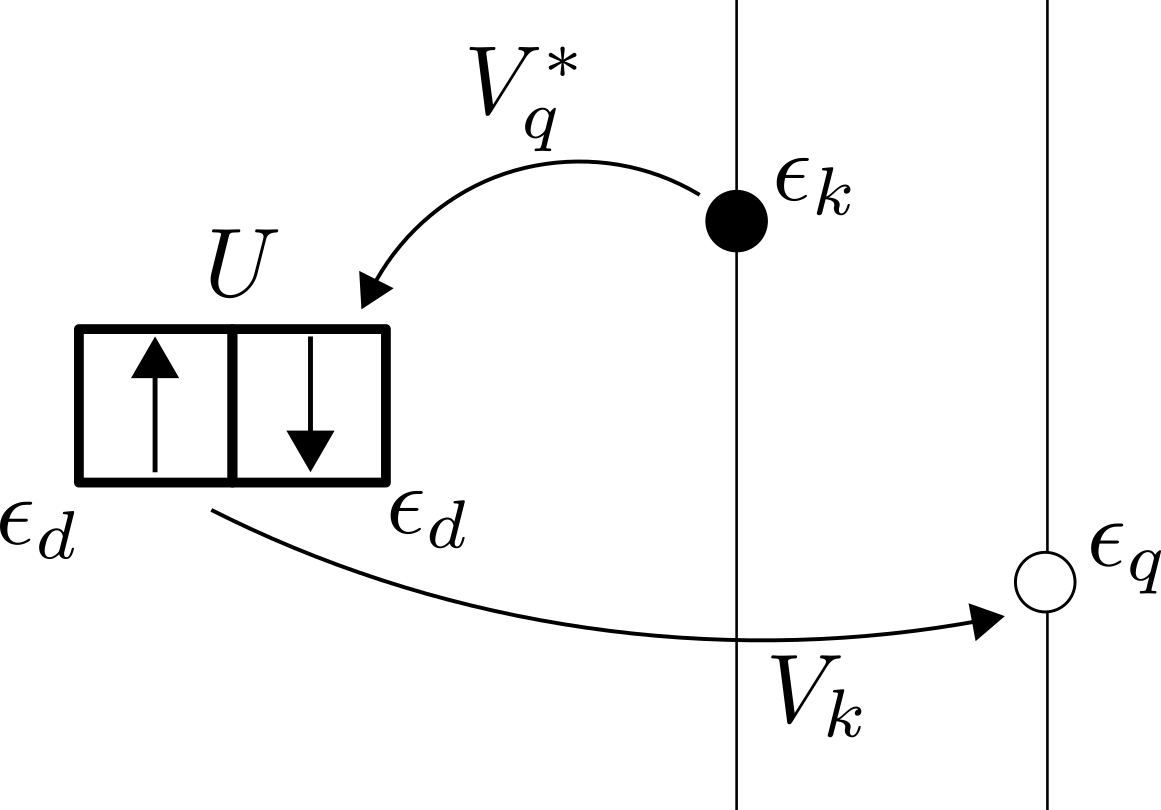
\includegraphics[scale=0.55]{model_scheme.png}
%\end{figure}
\only<+>{
\scalebox{1.38}{
	\hspace*{-10pt}\(\mathcal{H} = \overbrace{\sum_{k\sigma}\epsilon_k \hat n_{k\sigma}}^{\text{conduction}\atop{\text{bath}}} + \overbrace{\sum_{k\sigma}\left[V(k)c^\dagger_{k\sigma}c_{d\sigma} + \text{h.c.}\right]}^\text{hybridisation} + \overbrace{\epsilon_d \sum_\sigma \hat n_{d\sigma}}^{\text{impurity site}\atop{\text{energy}}} + \overbrace{U\hat n_{d\uparrow}\hat n_{d\downarrow}}^\text{d-d repulsion}
\)
}
\begin{minipage}{0.65\textwidth}
\begin{figure}
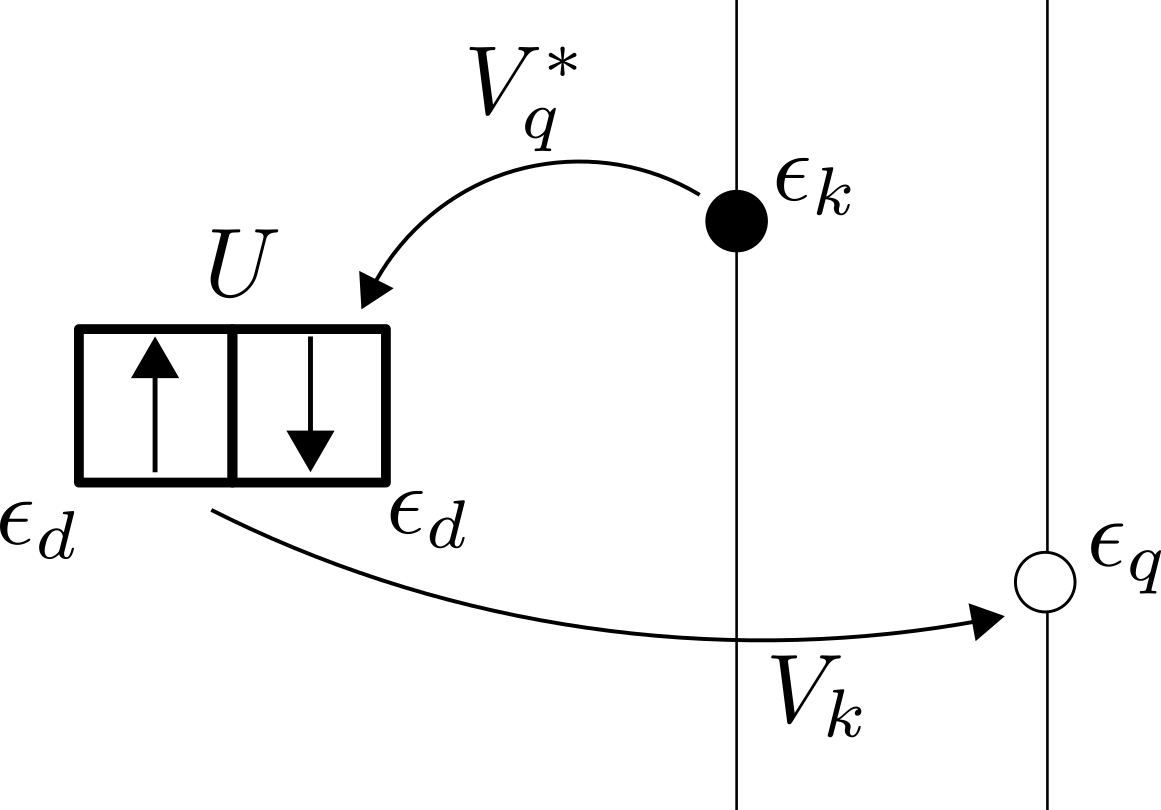
\includegraphics[scale=0.55]{model_scheme.png}
\end{figure}
\end{minipage}
\begin{minipage}{0.3\textwidth}
\begin{center}
	\LARGE{
		\[\rho(\epsilon) \approx \rho(\epsilon_F)\]\\[-25pt]
\[\Delta = \rho V^2\]\\[-25pt]
\[\epsilon_d = -\frac{1}{2}U\]
}
\end{center}
\end{minipage}
}
% \only<+>{
% 	\vspace*{-10pt}
% \cen{\Large\textbf{Poor Man's Scaling Results}}
% \begin{tabular}{cl}  
% \begin{tabular}{l}
%              \parbox{0.5\linewidth}{
% 		     For large \(U\), Haldane and Jefferson find\footnote{{Haldane-1978, Jefferson-1977, Hewson, A. C.-1993-The Kondo Problem to Heavy Fermions}} three low energy theories:
% \begin{itemize}
% 	\item the \textbf{frozen impururity fixed point} (\(\left<n_d\right> = 0\))
% 	\item the \textbf{local moment fixed point} (\(\left<n_d\right> = 1\)), and 
% 	\item the \textbf{valence fluctuation fixed point} (\(\left<n_d\right> \sim \frac{1}{2}\)).
% % Not much is reported about their stability, and the method itself is perturbative, so it breaks down before reaching the low energy theory.  
% \end{itemize}
%     }
%          \end{tabular}
%            &   \begin{tabular}{c}
% 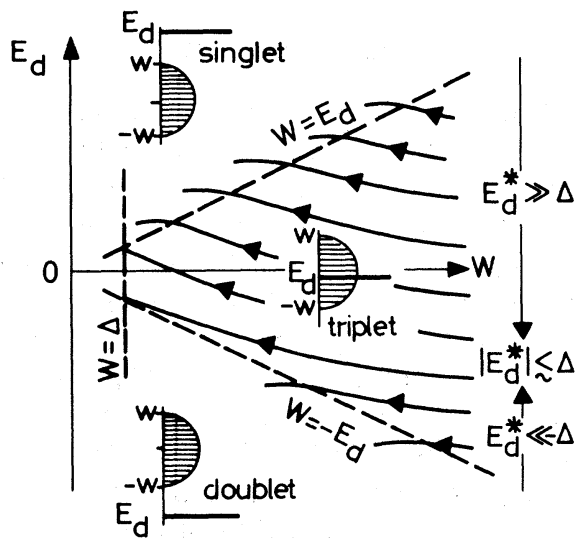
\includegraphics[scale=0.29]{haldane.png}
%            \end{tabular}\\
   
% \end{tabular}
% }
\only<+>{
\begin{tabular}{cl}  
\begin{tabular}{l}
             \parbox{0.5\linewidth}{
\cen{\Large\textbf{NRG Results - Symmetric Model}}
\begin{itemize}
\item the \focus{free-orbital} fixed point (\(U=\Delta=0\)) - unstable
		     \vspace*{10pt}
     \item the \focus{local moment} fixed point (\(U = \infty, \Delta=0\)) - saddle point, and 
		     \vspace*{10pt}
     \item the \focus{strong-coupling} fixed point (\(\Delta=\infty, U = \text{finite}\)) - stable.
\end{itemize}
    }
         \end{tabular}
           &   \begin{tabular}{c}
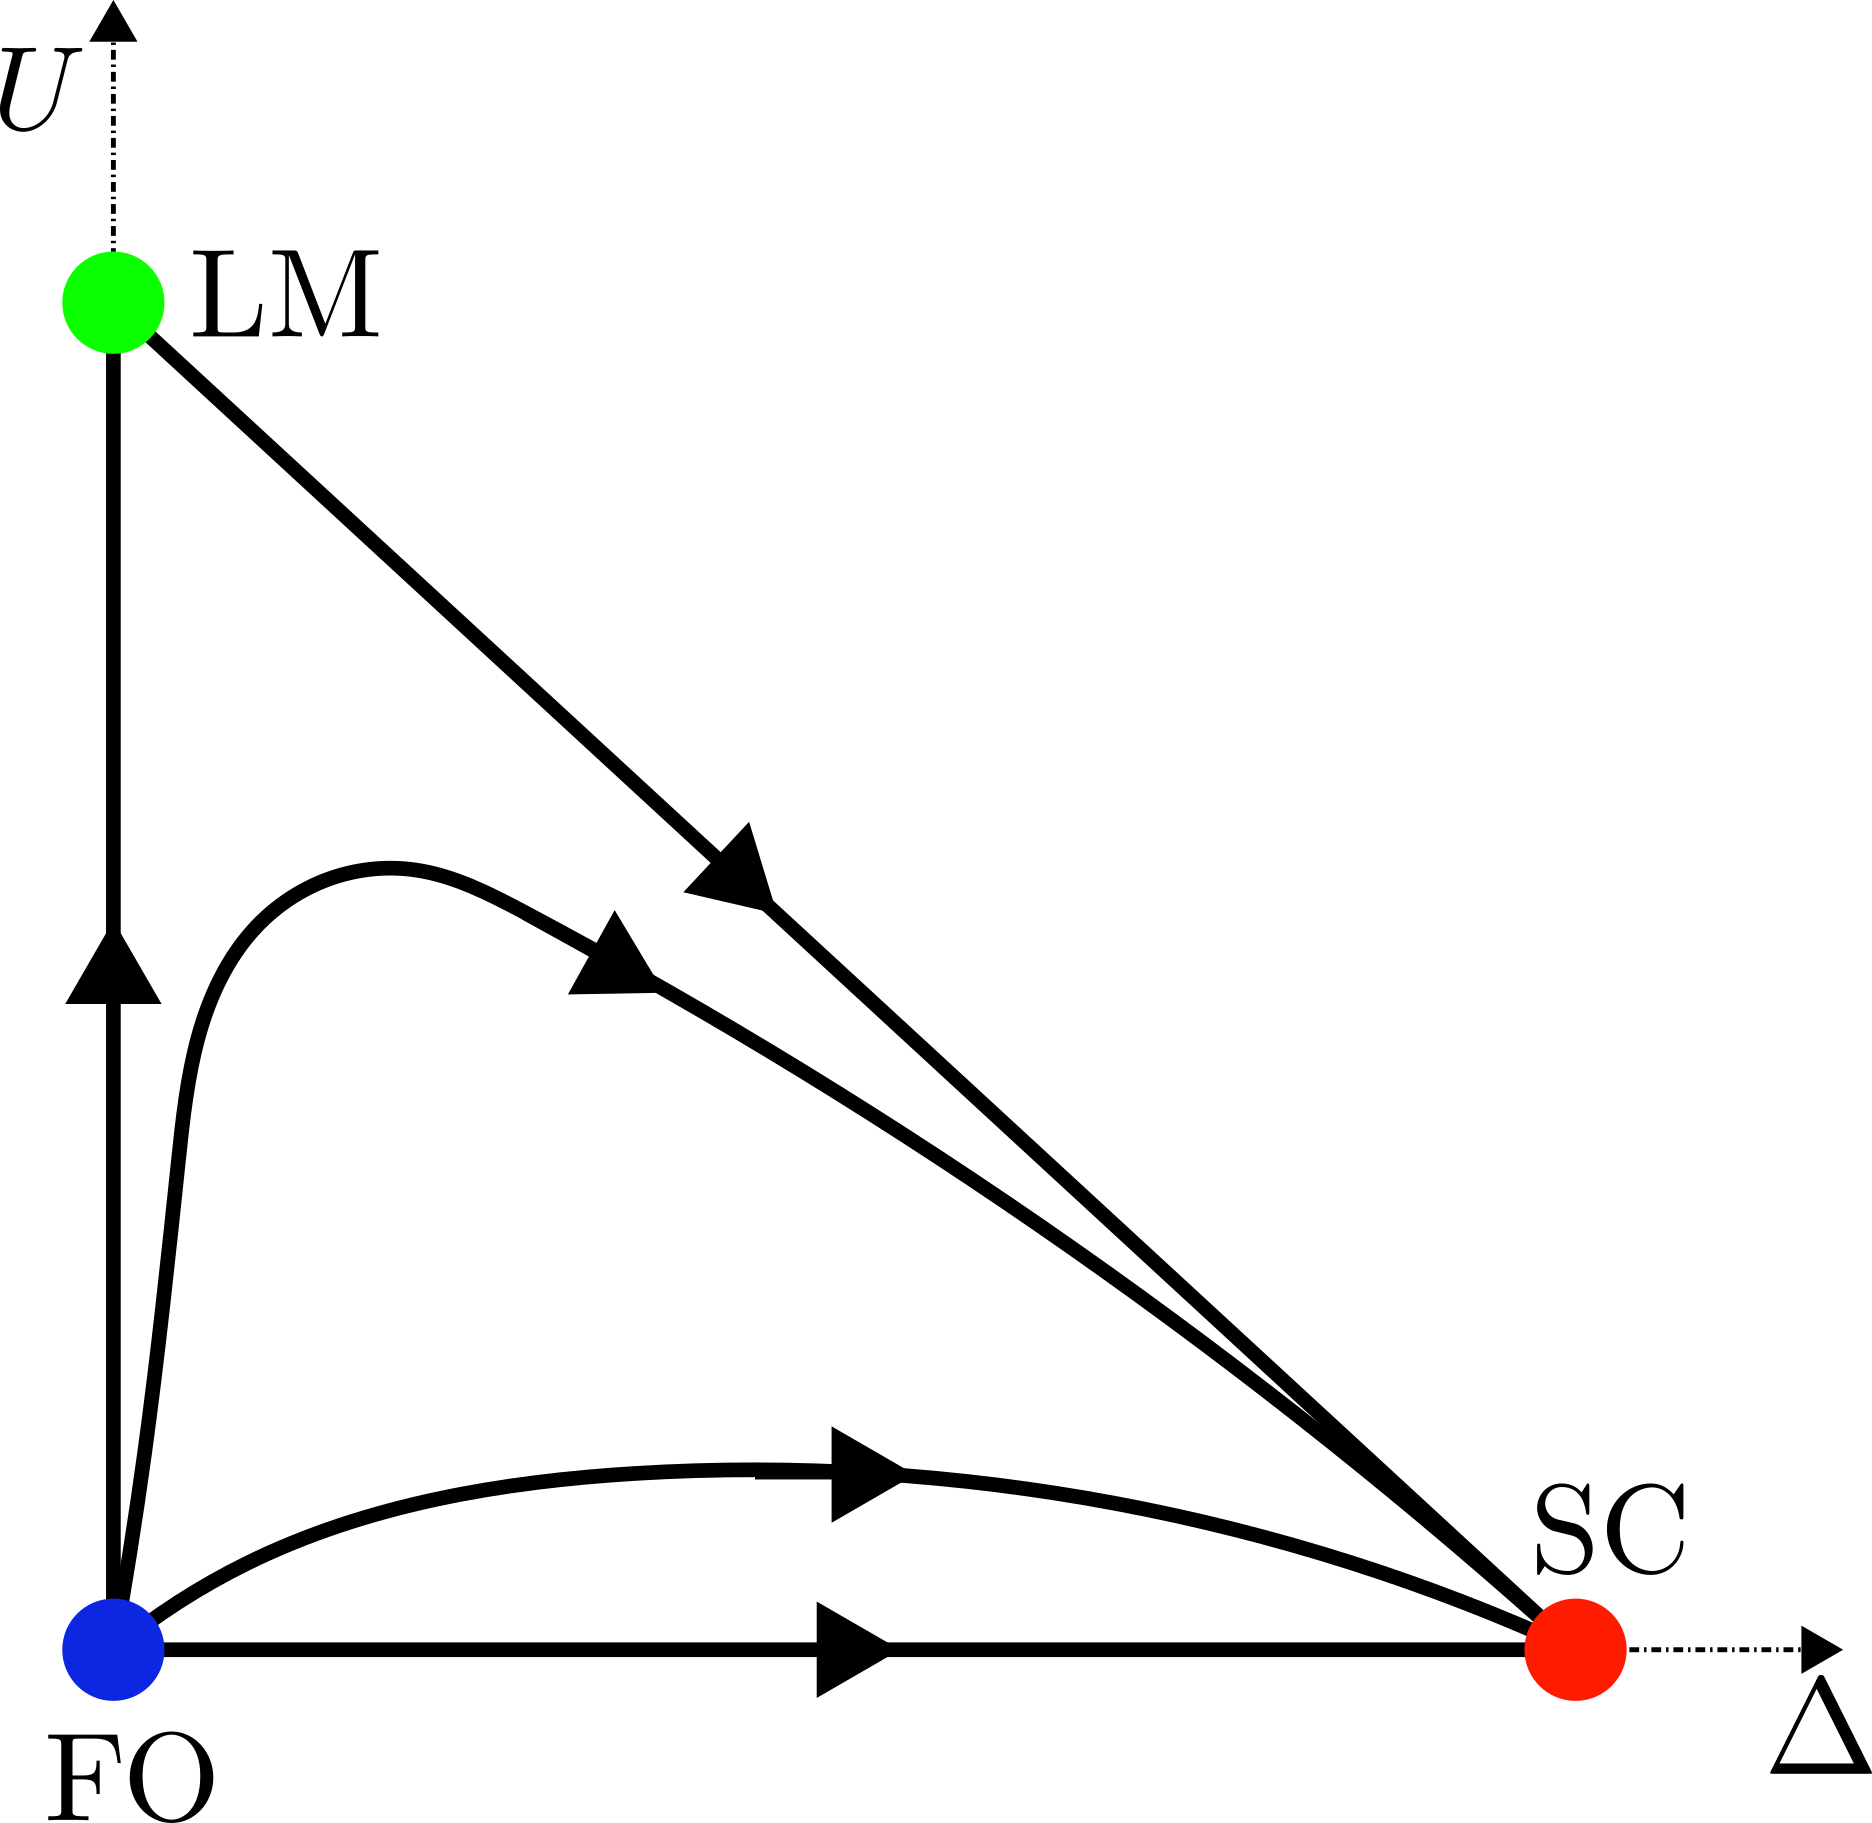
\includegraphics[scale=0.32]{nrg_fpoints.png}
           \end{tabular}\\
\end{tabular}
\footcite{hrk-nrg}
}
\end{frame}

\begin{frame}[noframenumbering]{Some Outstanding Questions}
  
\begin{itemize}
	\uncover<1->{\item Is it possible to get \focus{non-perturbative scaling equations} for the whole journey?}
	% \vspace*{10pt}
	% \uncover<2->{\item Can we get Hamiltonians and wavefunctions in the \textbf{crossover region} (\(T \sim T_K\))?}
	% \vspace*{10pt}
	\uncover<2->{\item What is the nature of the strong-coupling fixed point for a \focus{finite system} where \(J \neq \infty\)?
	% Will the results change if we introduce a \textbf{non-uniform density of states}?
	}
	% \vspace*{10pt}
	% \uncover<4->{\item Can we get \textbf{better estimates of dynamic quantities} in the crossover region?}
	% \vspace*{10pt}
	\uncover<3->{\item Is it possible to show the \focus{transfer of spectral weight} along the flow, possibly by tracking the spectral function?}
	\uncover<4->{\item How does the renormalization affect the \focus{many-particle entanglement} between the electrons?}
	% \vspace*{10pt}
	% \uncover<4->{\item How does NRG obtain the local moment in the \textbf{absence of hybridisation}?}
	% \vspace*{10pt}
	\uncover<5->{\item Are there any interesting \focus{topological aspects} of the fixed points?}
\end{itemize}

\end{frame}

%\begin{frame}[noframenumbering]{Motivation}
%  
%\begin{itemize}
%	\uncover<1->{\item "Poor man's" scaling\footnote{Haldane 1978, Jefferson 1977} is \textit{perturbative} and fails at large values - cannot show strong-coupling (SC) fixed point.}
%	\vspace*{20pt}
%	\uncover<2->{\item Instead, one needs to flow to large value of \(U\), do a Schrieffer -Wolff transformation and then flow to the SC fixed point. }
%	\vspace*{20pt}
%	\uncover<3->{\item \textbf{It would be nice to get a single set of equations that show the crossover to the strong-coupling fixed point.}}
%\end{itemize}
%
%\end{frame}
%
%\begin{frame}[noframenumbering]{Motivation}
%
%\begin{itemize}
%	\uncover<1->{\item Numerical Renormalization Group (NRG) does not provide any scaling equations - hard to figure out what is really happening.}
%	\vspace*{20pt}
%	\uncover<2->{\item NRG cannot show \textit{how the Hamiltonians and many-body wavefunctions vary along the flow} - projective in nature.}
%	\vspace*{20pt}
%	\uncover<3->{\item \textbf{It would be enlightening to see the flow into SC regime by tracking the change in entanglement} - hence we need wavefunctions.}
%\end{itemize}
%\end{frame}

\begin{frame}[noframenumbering]{Unitary Renormalization Group: Overview}

	\only<+>{\begin{minipage}{200pt}\cen{\textbf{The Short Version}}Apply \textit{unitary many-body transformations} to the Hamiltonian so as to successively \textit{decouple} high energy states and hence obtain scaling equations.\end{minipage}\begin{minipage}{250pt}\begin{figure}
\def\svgwidth{\columnwidth}
\centering
\scalebox{0.5}{\input{urg_short.pdf_tex}}
\end{figure}\end{minipage}}
\footcite{holography1}
\end{frame}
\begin{frame}[noframenumbering]{URG: Formalism}
\only<+>{\begin{minipage}{200pt}\cen{\large{\textbf{Step 1:}}}Start with the electrons farthest from the Fermi surface. Write the Hamiltonian as \textit{diagonal and off-diagonal terms} in this basis.\end{minipage}\begin{minipage}{300pt}
	\begin{figure}
\def\svgwidth{\columnwidth}
\centering
\input{matrix.pdf_tex}
\end{figure}
\end{minipage}}
\only<+>{\cen{\large{\textbf{Step 2:}}\\Rotate the Hamiltonian to kill the off-diagonal blocks.}
\begin{figure}
\def\svgwidth{\columnwidth}
\centering
\input{rotation.pdf_tex}
\end{figure}
% mention the commutator here
}
\only<+>{\cen{\large{\textbf{Step 3:}}\\Repeat the process with the new blocks.}
\begin{figure}
\def\svgwidth{\columnwidth}
\centering
\input{repeat.pdf_tex}
\end{figure}}
\end{frame}
\begin{frame}[noframenumbering]{URG: Salient Features}
\vspace*{\fill}
\begin{itemize}
	\item Presence of the quantum fluctuation energy scale \(\omega\)
\vspace{10pt}
	\item Presence of finite-valued fixed points
\vspace{10pt}
	\item Spectrum-preserving transformations
\vspace{10pt}
	\item Tractable low-energy effective Hamiltonians
\end{itemize}
\vspace*{\fill}
\end{frame}

\begin{frame}[noframenumbering]{URG: Relation to Poor Man's Scaling}
	\vspace*{-50pt}
	\begin{center}
		\Large\[H = H_0 + \underbrace{V_+ + V_-}_{\text{off-diagonal terms} \atop{\text{we want to remove}}}\]
	\end{center}
\only<+>{
\begin{minipage}{0.45\textwidth}
\begin{figure}[htpb]
	\centering
	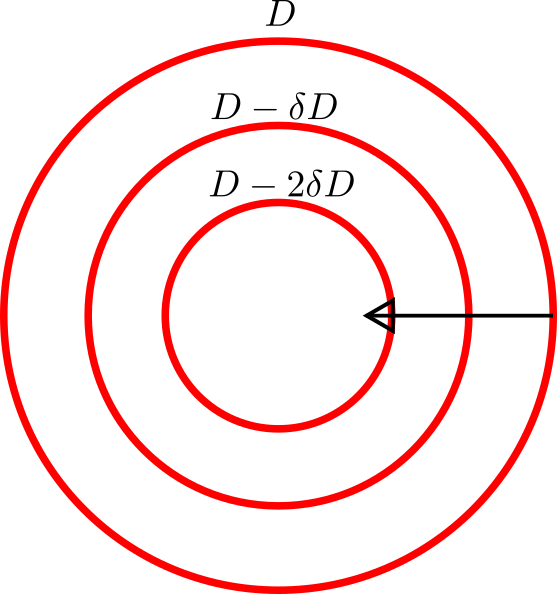
\includegraphics[width=0.7\textwidth]{figures/pms.png}
\end{figure}
\end{minipage}
\hspace*{20pt}
\begin{minipage}{0.45\textwidth}
Philosophy of Poor Man's scaling:
\begin{itemize}
	\item Successively eliminate high-energy energy shells
	\item Write high energy excitations as second-order correction to low-energy scatterings
	\item Typically perturbative
\end{itemize}
\end{minipage}
\footcite{Anderson}
}
\only<+>{\begin{minipage}{0.5\textwidth}
\[\Delta H_\text{PMS} = V_- \frac{1}{E - H_0}V_+ + V_+ \frac{1}{E - H_0}V_-\]
\begin{center}
	\large\(\Bigg\downarrow E \to \omega\)
\end{center}
\[\Delta H_\text{URG} = V_- \frac{1}{\omega - H_0}V_+ + V_+ \frac{1}{\omega - H_0}V_-\]
\end{minipage}
\begin{minipage}{0.49\textwidth}
\begin{figure}[htpb]
	\centering
	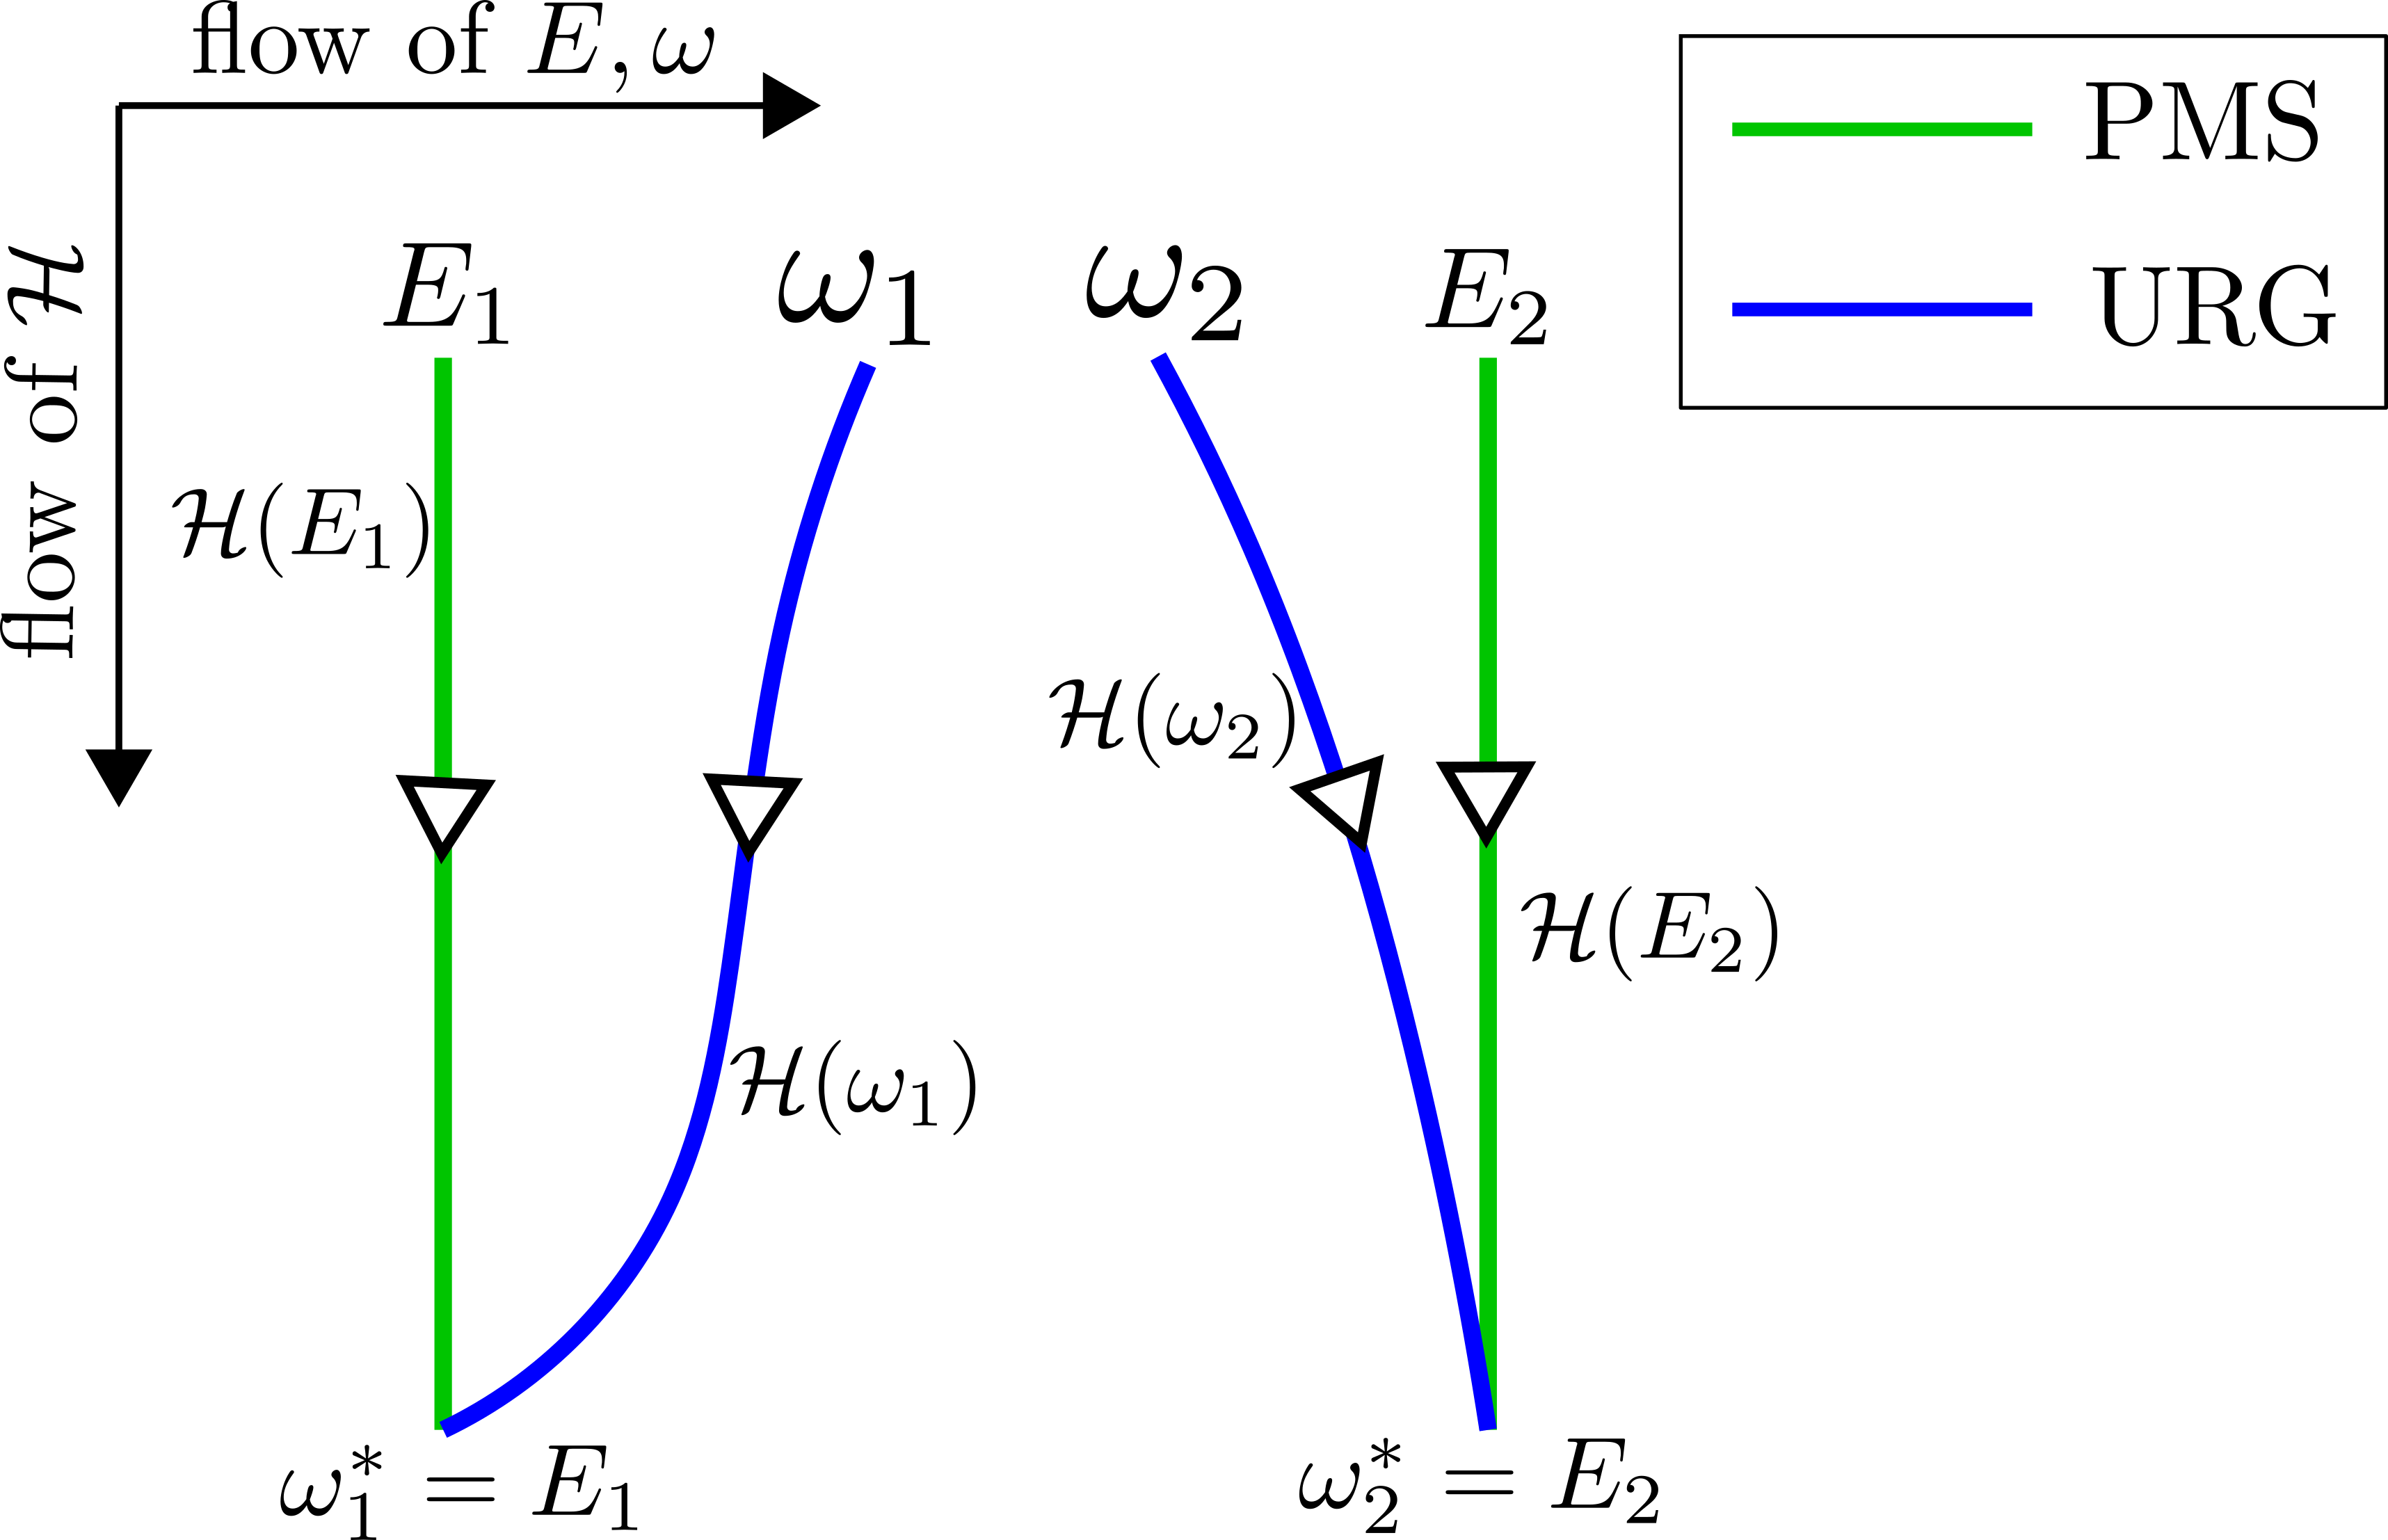
\includegraphics[width=0.9\textwidth]{figures/pms_vs_urg.png}
\end{figure}
\end{minipage}
}
\end{frame}
\begin{frame}[noframenumbering]{URG: Relation to Continuous Unitary Transformation RG}
\Large\[H = \overbrace{H_d}^\text{diagonal part} + \overbrace{H_X}^\text{off-diagonal part}\]
\begin{center}
	\Large$\Delta H_\text{CUT} = \Delta l\bigg[\big[H_d(l), H_X(l)\big], H(l)\bigg]$
\end{center}
\vspace*{20pt}
\only<+>{
	\begin{minipage}{0.39\textwidth}
		{\Large\(V_{kq}(l) = V_{kq}(0)e^{\left( \epsilon_k - \epsilon_q \right) l}\)}
\end{minipage}
\hspace*{0.09\textwidth}
\begin{minipage}{0.5\textwidth}
	\large{
	\begin{itemize}
		\item off-diagonal terms decay exponentially
			\vspace*{10pt}
		\item those that connect larger energy differences decay fastest
	\end{itemize}
}
\end{minipage}
\begin{center}
\end{center}
\footcite{glazek-wilson}
}
\only<+>{
	\vspace*{-10pt}
\begin{center}
	\large\(\Delta H_\text{URG} = \overbrace{\bigg[\big[H_d, \frac{1}{\omega_1 - \omega_0} \left( \hat \omega - H_d \right)^{-1} H_I\big], H\bigg]}^{\Delta H_0} - H^I\)\\[20pt]
	\large\(\Delta H_0 \xrightarrow{\left( \hat \omega - H_d \right)^{-1} \sim -H_d^{-1}} \Delta \lambda \times \bigg[\big[H_d, H_I\big], H\bigg]\)
\end{center}
}
\end{frame}

\begin{frame}[noframenumbering]{Model: Generalized SIAM}
\begin{center}
\scalebox{1.3}{\(H = H_\text{SIAM} + J \vec{S_d}\cdot\vec{s} + K \vec{C_d}\cdot\vec{c}\)}
\end{center}
\vspace*{30pt}
\hspace*{\fill}\(\vec{S_d} \equiv \frac{1}{2}\sum_{\alpha\beta}c^\dagger_{d\alpha}\vec{\sigma}_{\alpha\beta}c_{d\beta}\)\hspace*{\fill}\(\vec{s} \equiv \frac{1}{2}\sum_{\alpha\beta}c^\dagger_{0\alpha}\vec{\sigma}_{\alpha\beta}c_{0\beta}\)\hspace*{\fill}
\\
\vspace*{15pt}
\hspace*{\fill}\(\vec{C_d} \equiv \frac{1}{2}\sum_{\alpha\beta}\psi^\dagger_{d\alpha}\vec{\sigma}_{\alpha\beta}\psi_{d\beta}\)\hspace*{\fill}\(\vec{c} \equiv \frac{1}{2}\sum_{\alpha\beta}\psi^\dagger_{0\alpha}\vec{\sigma}_{\alpha\beta}\psi_{0\beta}\)\hspace*{\fill}
\\
\vspace*{15pt}
\hspace*{\fill}\(\vec{\psi}_d \equiv \begin{pmatrix} c_{d \uparrow} \\ c^\dagger_{d \downarrow}\end{pmatrix} \)\hspace*{\fill}\(\vec{\psi}_0 \equiv \sum_k \begin{pmatrix} c_{k \uparrow} \\ c^\dagger_{k \downarrow}\end{pmatrix}\)\hspace*{\fill}
\footcite{Schrieffer_Wolff}
\end{frame}

\begin{frame}[noframenumbering]{Results: RG Equations}
\[
\Delta U = 4|V|^2 \left[\frac{1}{\omega - \frac{1}{2}D + \frac{U}{2} + \frac{1}{2}J}  - \frac{1}{\omega - \frac{1}{2}D - \frac{U}{2} + \frac{1}{2}K}\right] + \sum_{k<\Lambda_j} \frac{3}{4}\frac{K^2 - J^2}{\omega - \frac{1}{2}D + \frac{1}{4}J + \frac{1}{4}K}
\]

\[
	\hspace*{-10pt}\Delta V = \frac{V K}{16}\left(\frac{1}{\omega - \frac{1}{2}D - \frac{U}{2} + \frac{1}{2}K} + \frac{1}{\omega - \frac{1}{2}D + \frac{1}{4}J + \frac{1}{4}K} \right) - \frac{3VJ}{4}\left( \frac{1}{\omega - \frac{1}{2}D + \frac{U}{2} + \frac{1}{2}J} + \frac{1}{\omega - \frac{1}{2}D + \frac{1}{4}J + \frac{1}{4}K} \right)
\]

\[
\Delta J = - J^2\left(\omega - \frac{1}{2}D + \frac{1}{4}J + \frac{1}{4}K\right)^{-1}
\]

\[
\Delta K = - K^2\left(\omega - \frac{1}{2}D + \frac{1}{4}J + \frac{1}{4}K\right)^{-1}
\]
\end{frame}

\begin{frame}[noframenumbering]{Results: \(U>0, J>K\)}
\begin{minipage}{0.6\textwidth}
\begin{center}
	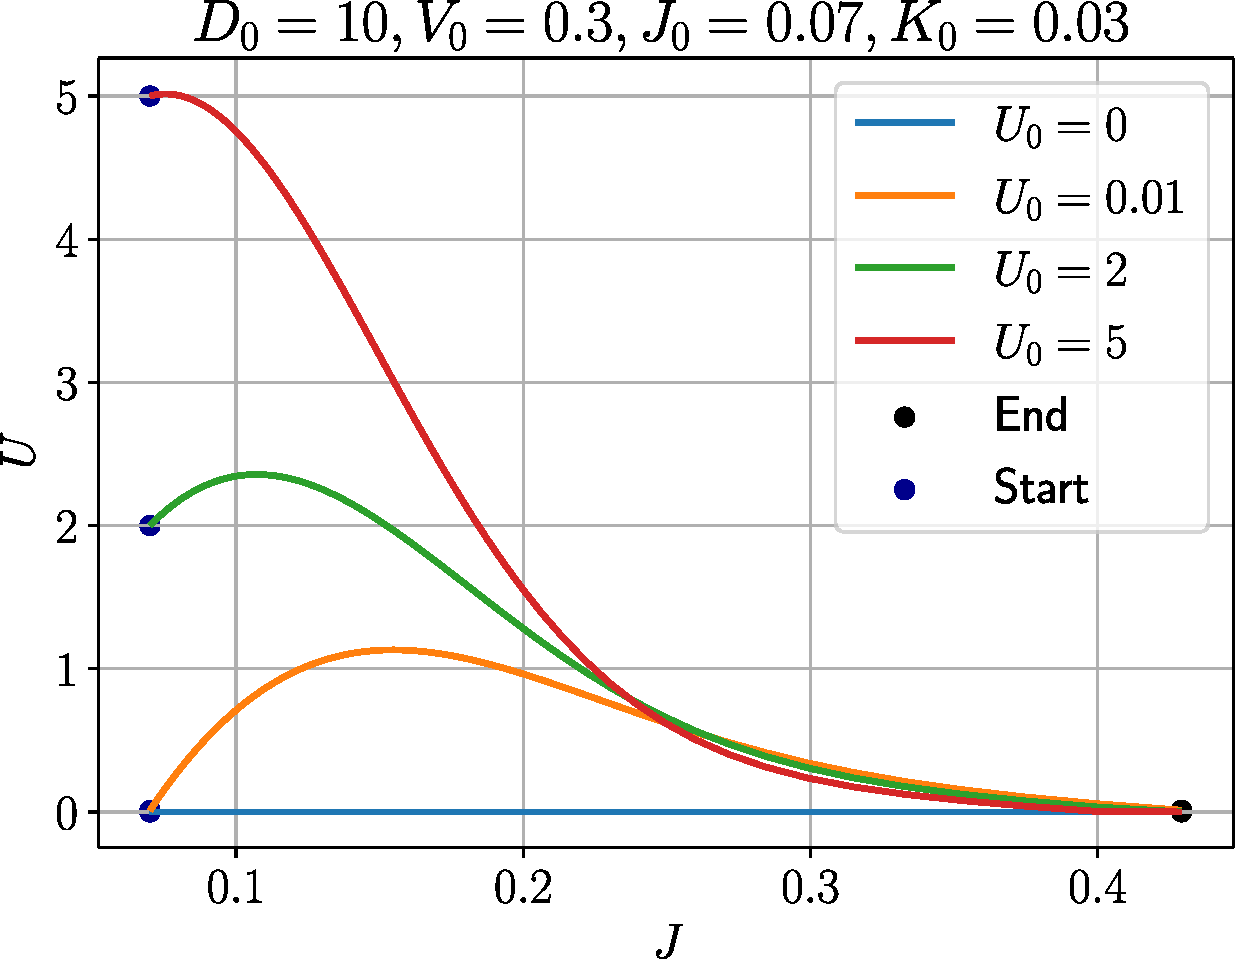
\includegraphics[width=\textwidth]{figures/UvsJ.pdf}
\end{center}
\end{minipage}
\begin{minipage}{0.39\textwidth}
\begin{center}
	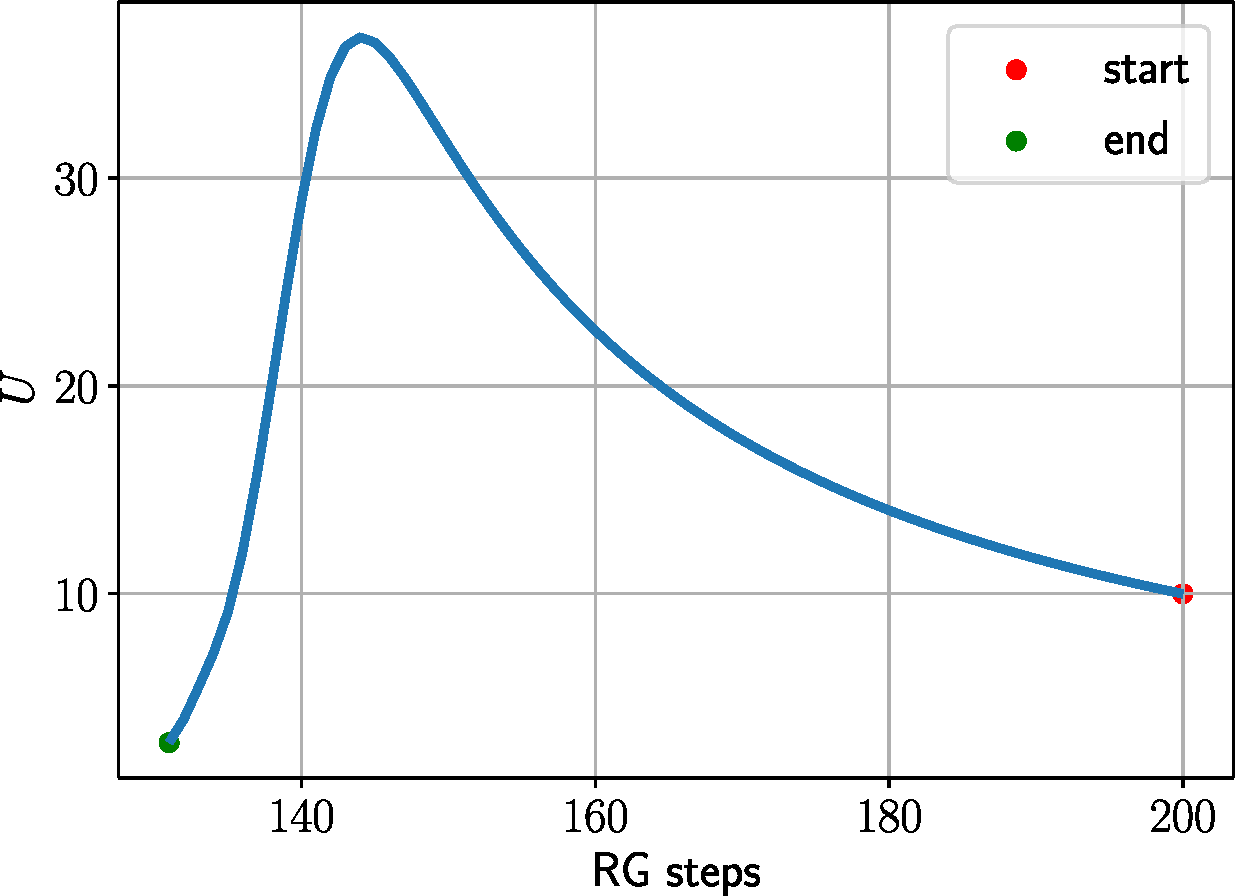
\includegraphics[width=0.95\textwidth]{figures/U_vs_count.pdf}
	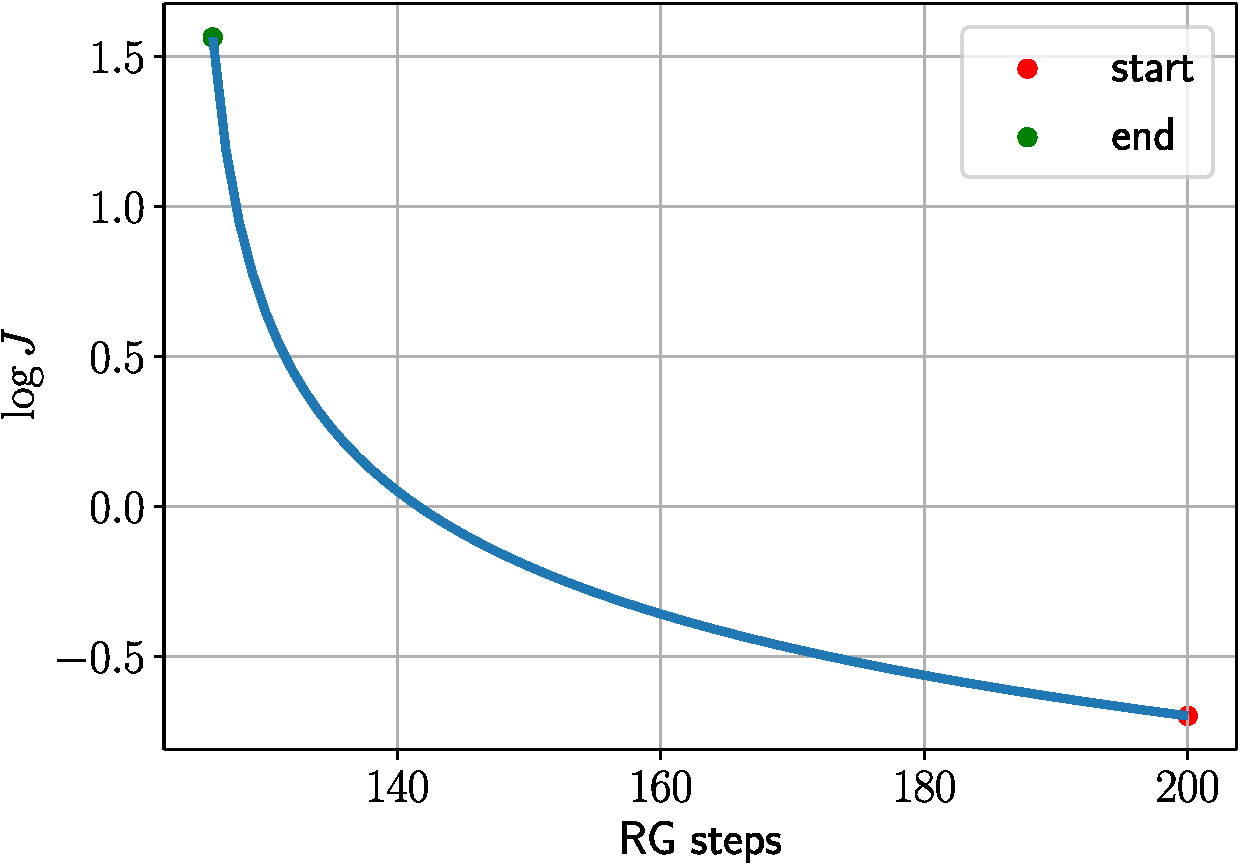
\includegraphics[width=0.95\textwidth]{figures/J_vs_count.pdf}
\end{center}
\end{minipage}
\end{frame}


\begin{frame}[noframenumbering]{Results: \(U<0, J<K\)}
	\vspace*{30pt}
\begin{center}
	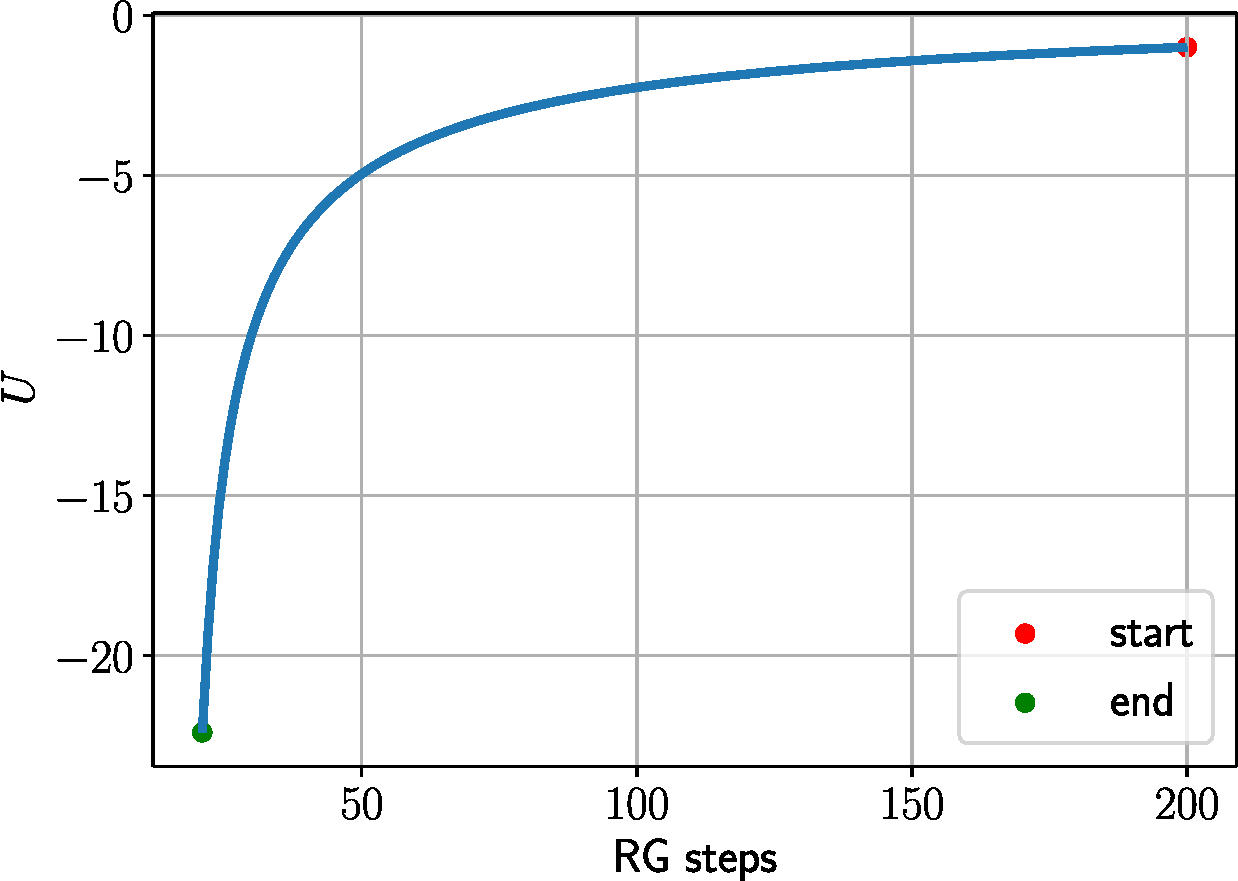
\includegraphics[width=0.49\textwidth]{figures/U_vs_count_neg.pdf}
	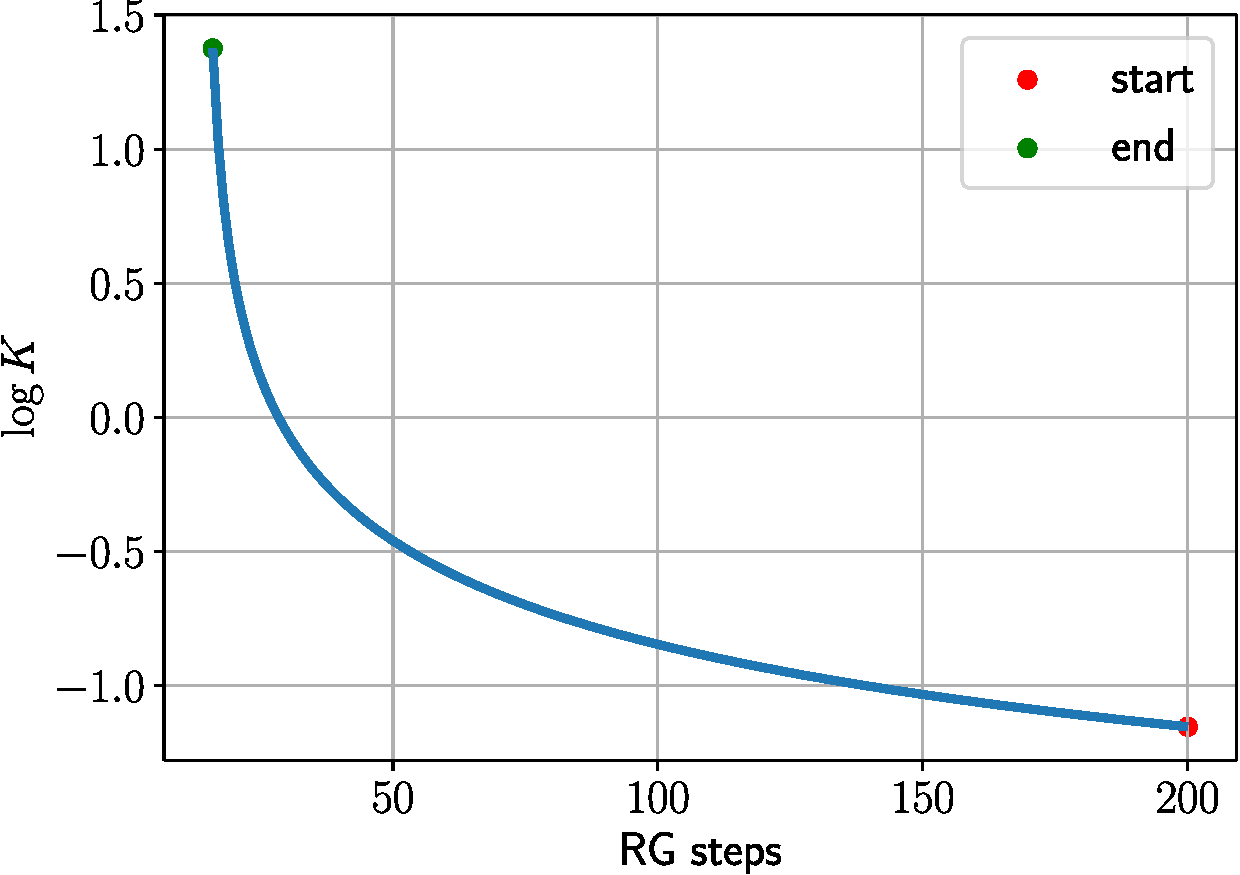
\includegraphics[width=0.49\textwidth]{figures/K_vs_count_neg.pdf}
\end{center}
\end{frame}


\begin{frame}[noframenumbering]{Results: Phase Diagram}
\begin{center}
	\hspace*{-50pt}\def\svgwidth{0.8\columnwidth}
	\input{phases-V-pres.pdf_tex}
	% 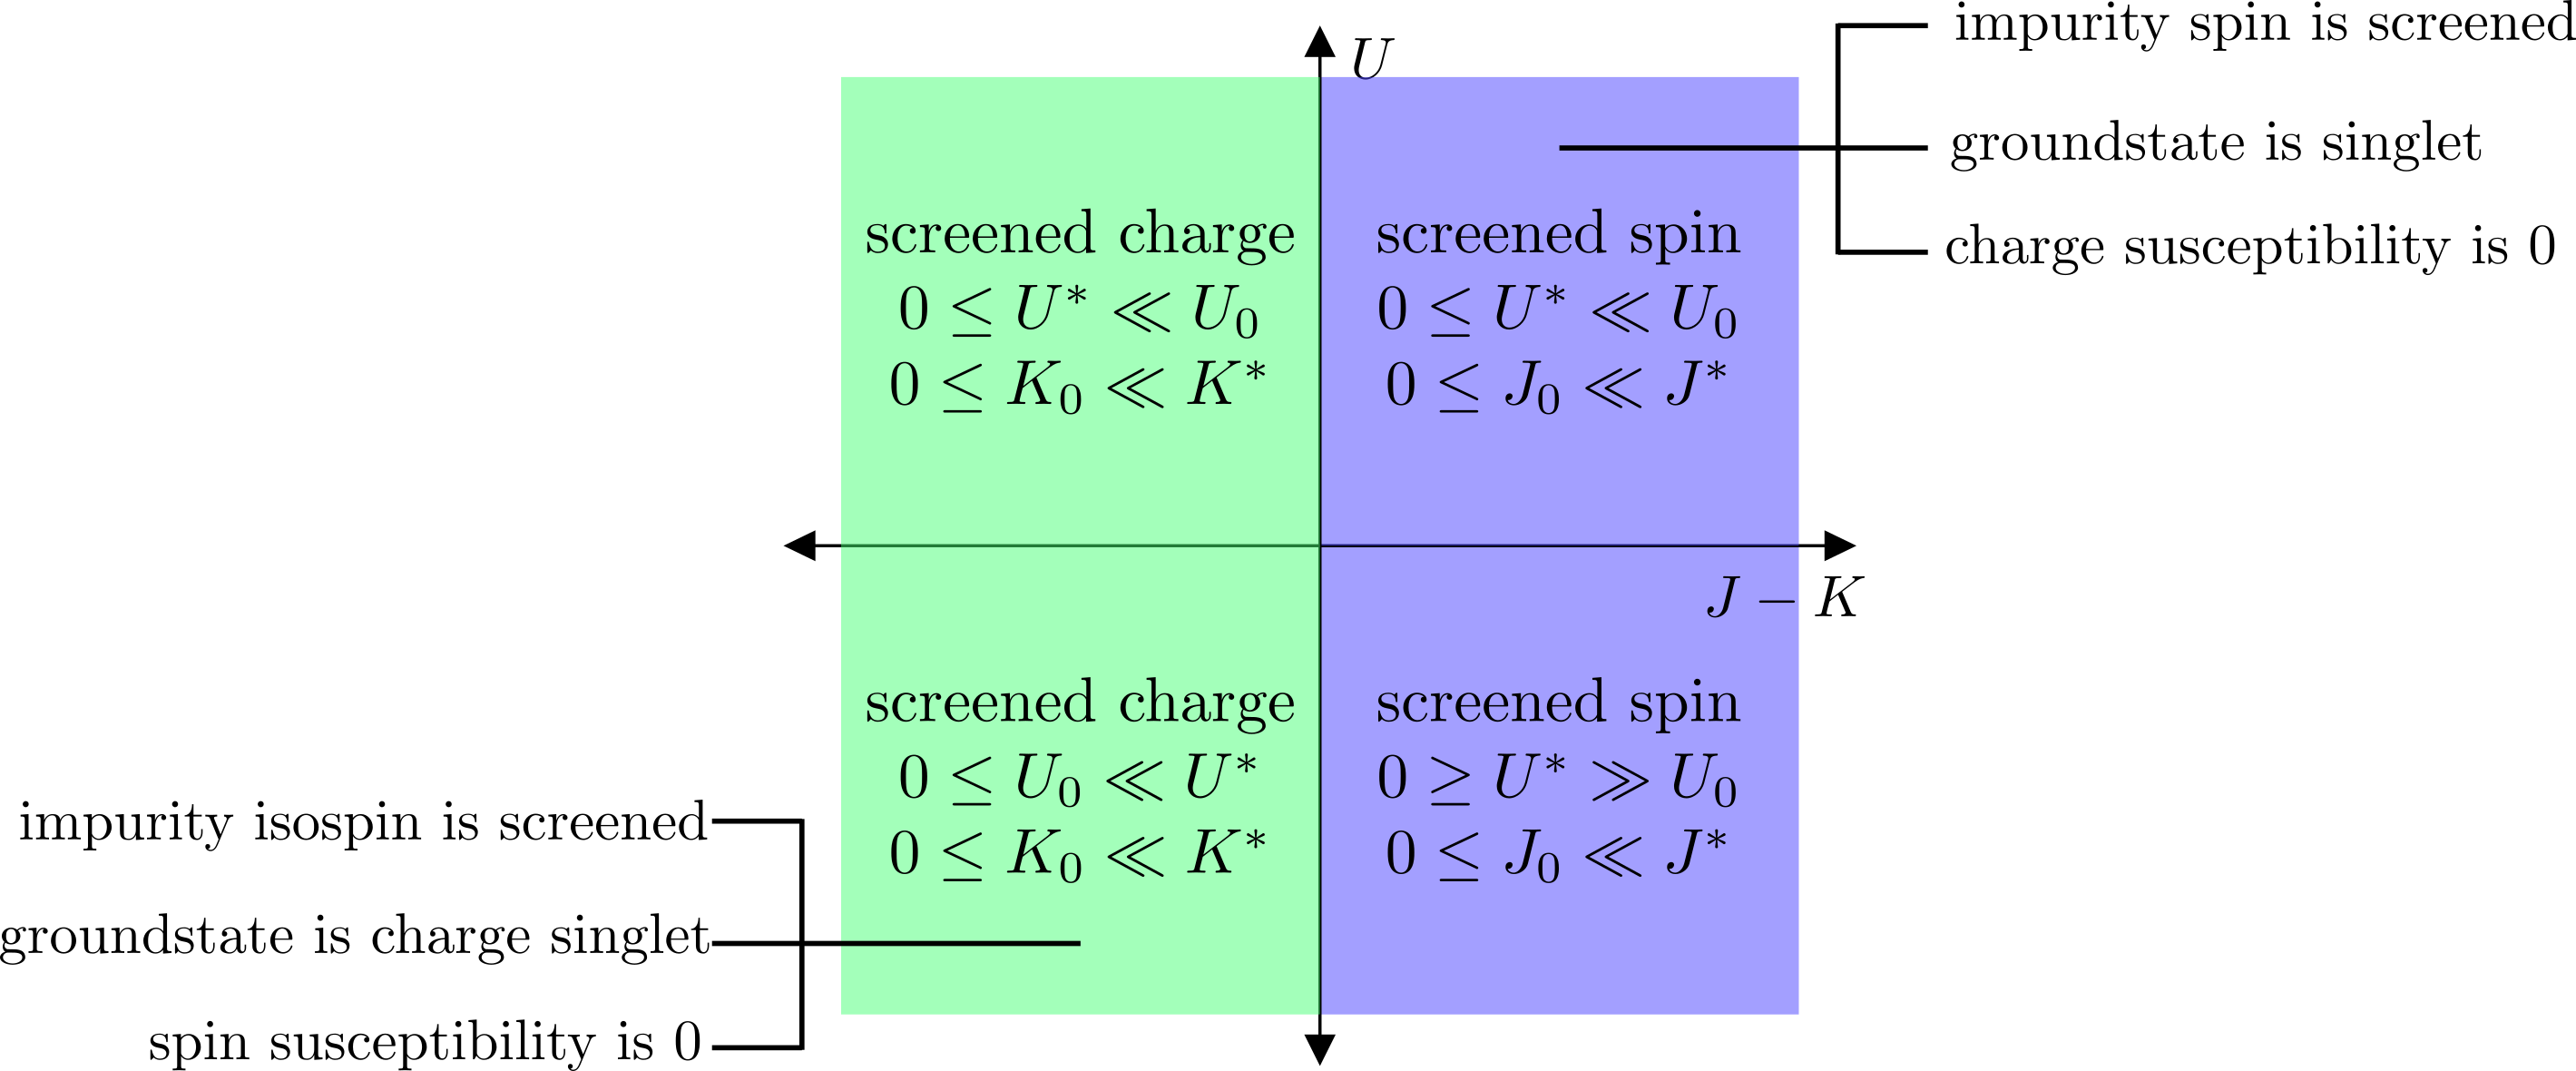
\includegraphics[width=0.99\textwidth]{figures/phases_V_pres.png}
\end{center}
\end{frame}


\begin{frame}[noframenumbering]{Results: Effective Zero-mode Hamiltonian}
	\vspace*{-30pt}
	\[H_{IR} = \epsilon_d^* \left( \hat n_{1 \uparrow} - \hat n_{1 \downarrow} \right) ^2 + V^*\sqrt{N^*}\sum_{\sigma}\left(c^\dagger_{1\sigma}c_{2\sigma} + \text{h.c.} \right) + J^*N^*\vec{S_1}\cdot\vec{S_2} + K^*N^*\vec{C_1}\cdot\vec{C_2}\]
\hspace*{-15pt}
	\begin{minipage}{0.5\textwidth}
	{\centering
	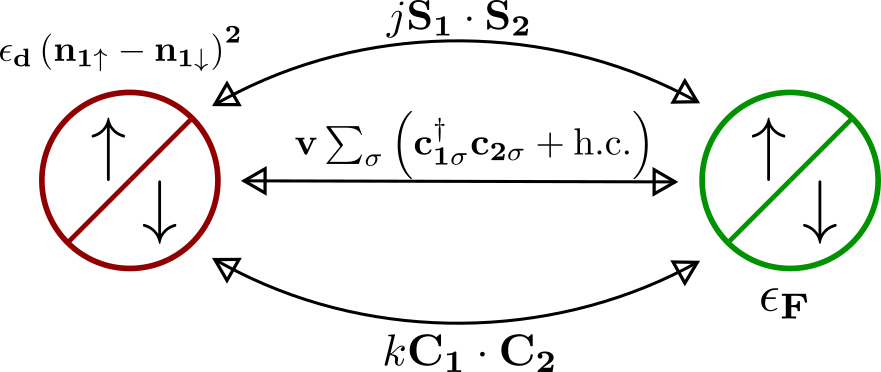
\includegraphics[width=\textwidth]{figures/two_site_problem.png}}
\end{minipage}
\hspace*{25pt}
\begin{minipage}{0.45\textwidth}
	{\centering
	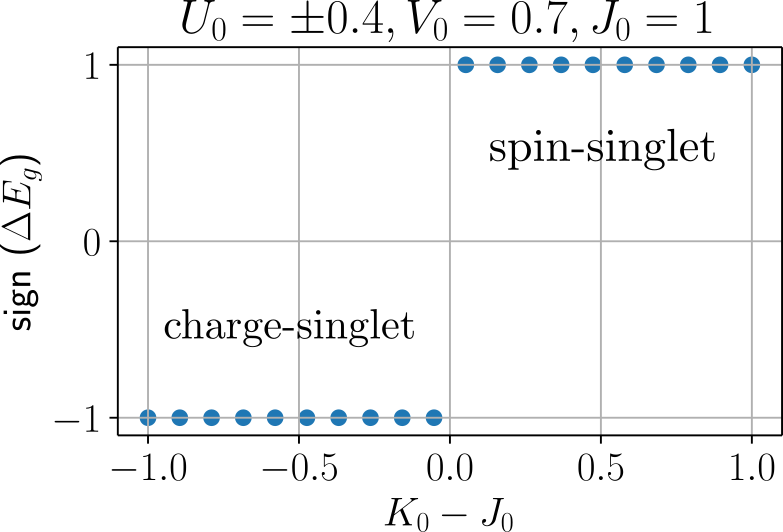
\includegraphics[width=\textwidth]{figures/gstate_state.png}}
\end{minipage}

\footcite{wilson,hrk-nrg,taraphder}

\end{frame}

\begin{frame}[noframenumbering]{Results: Ground State}
\begin{minipage}{0.65\textwidth}
	\[J > K, U>0\]
\vspace*{-10pt}
	\[\ket{\Psi}_\text{GS} = c_-^s\left[\ket{\uparrow, \Downarrow} - \ket{\downarrow, \Uparrow}\right] + c_-^c\left[\ket{\uparrow, \Downarrow} + \ket{\downarrow, \Uparrow}\right]\]

\vspace*{10pt}
\begin{minipage}{0.65\textwidth}
\begin{figure}[htpb]
	\centering
	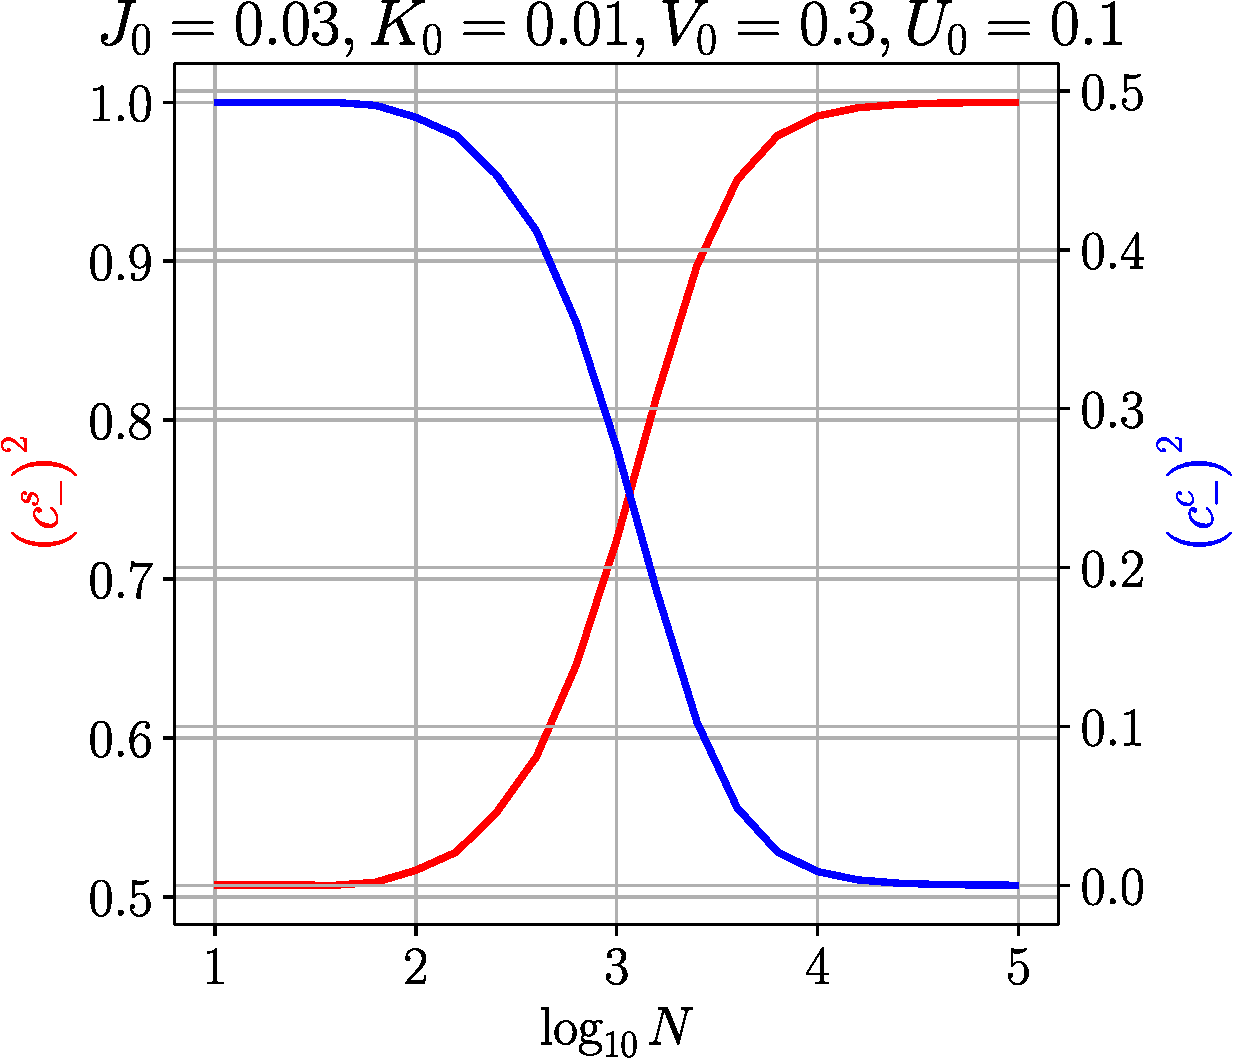
\includegraphics[width=0.8\textwidth]{figures/cscc_q1.pdf}
\end{figure}
\end{minipage}
\begin{minipage}{0.3\textwidth}
	\[ c_-^s \to 1\]
	\[ c_-^c \to 0\]
\end{minipage}
\[\ket{\Psi}_\text{GS} \sim \left[\ket{\uparrow, \Downarrow} - \ket{\downarrow, \Uparrow}\right]\]
\end{minipage}
\vline
\begin{minipage}{0.34\textwidth}
\[J < K, U<0\]
\[\ket{\Psi}_\text{GS} = \left[\ket{\uparrow_c, \Downarrow_c} - \ket{\downarrow_c, \Uparrow_c}\right]\]
\vspace*{0.6\textheight}
\end{minipage}
\end{frame}

\begin{frame}[noframenumbering]{Results: Spin Susceptibility}
	\vspace*{-20pt}
	\[\chi_s = \lim_{B \to 0} \frac{\partial{m}}{\partial{B}}\]
\begin{center}
	\hspace*{-20pt}
	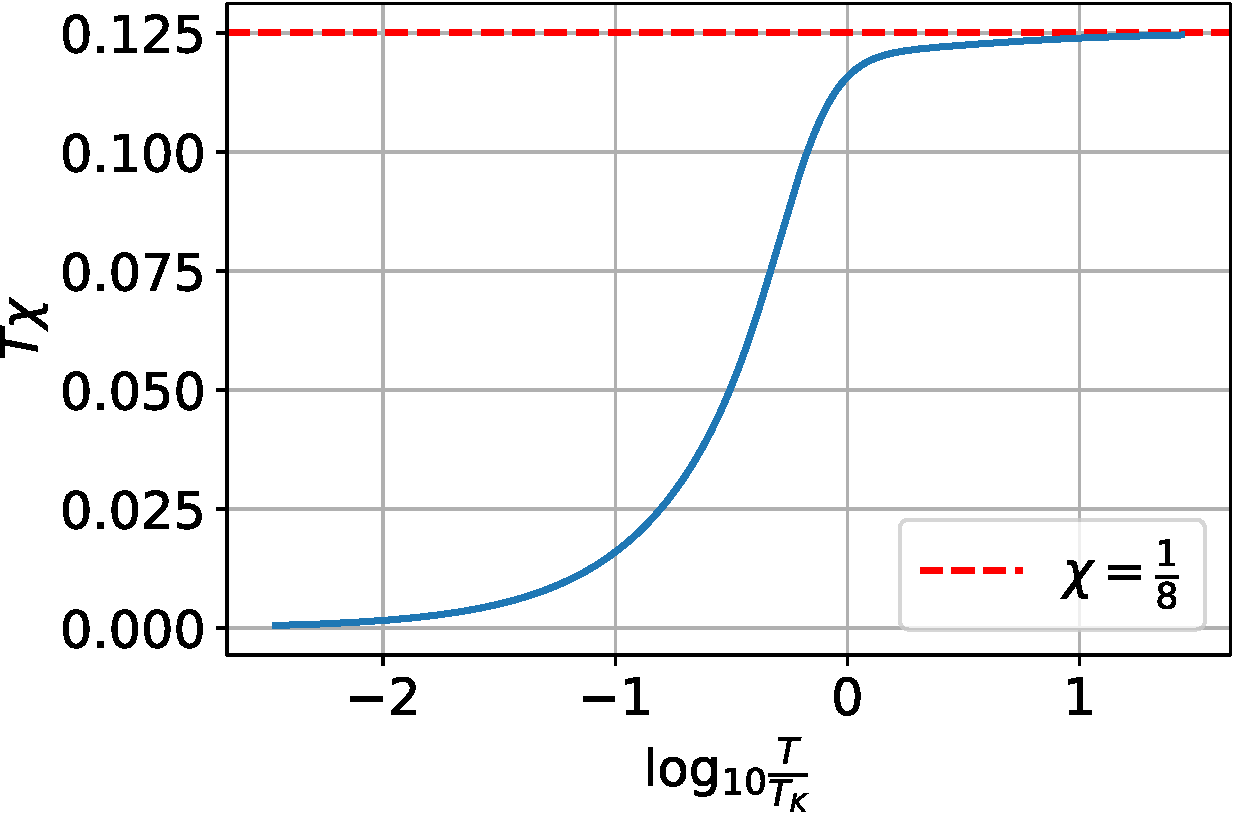
\includegraphics[width=0.48\textwidth]{figures/chi_T.pdf}
	\hspace*{25pt}
	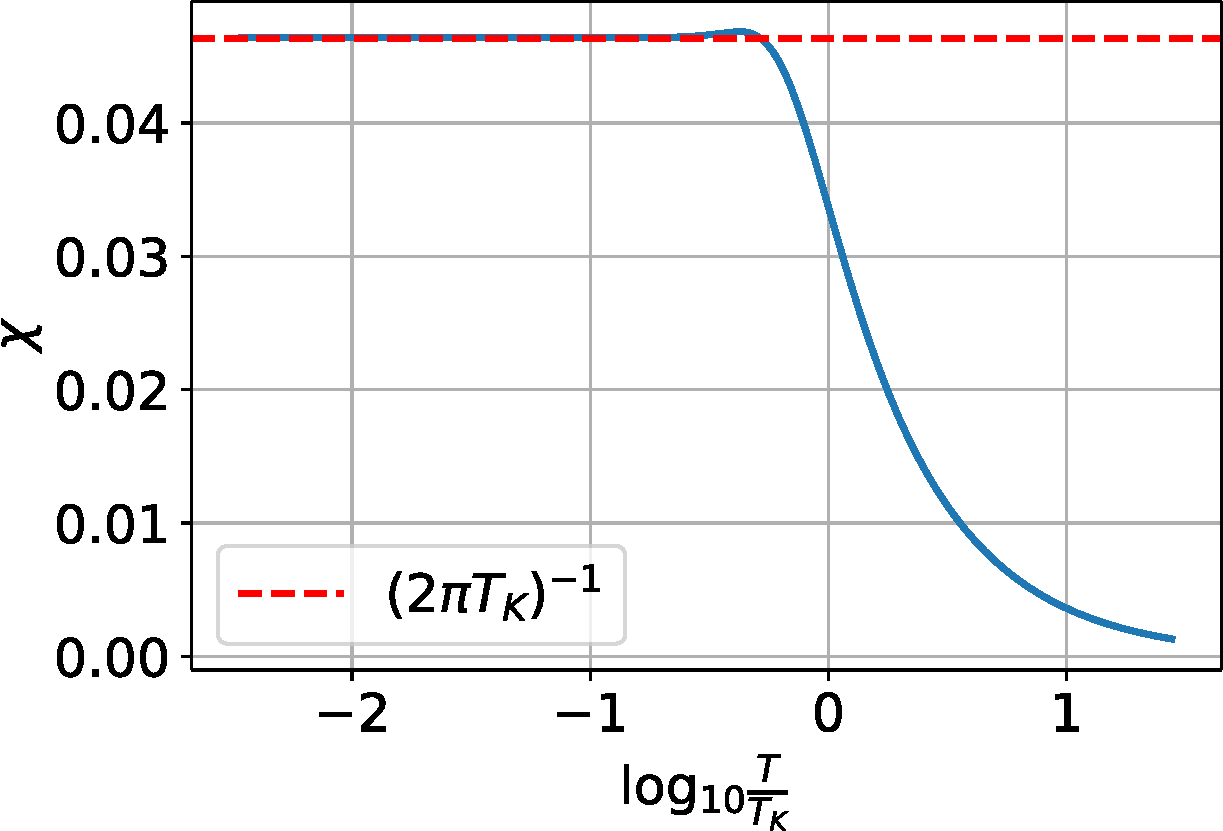
\includegraphics[width=0.48\textwidth]{figures/chi.pdf}
\end{center}
\hspace*{20pt}\large{\(
\left(\chi\times T\right)\left( T \to 0 \right) = \frac{1}{2j} \hspace*{\fill} T_K \equiv \frac{2N^*}{\pi}\left(D^* - 2\omega\right)\hspace*{\fill} \chi \left( T \to \infty \right) = \frac{1}{8}\)}

\footcite{wilson, hrk-nrg}
\end{frame}

\begin{frame}[noframenumbering]{Results: Charge Susceptibility}
	\vspace*{-15pt}
	\[\chi_c = \lim_{\mu \to 0} \frac{\partial{N}}{\partial{\mu}}\]
\begin{center}
	\hspace*{-20pt}
	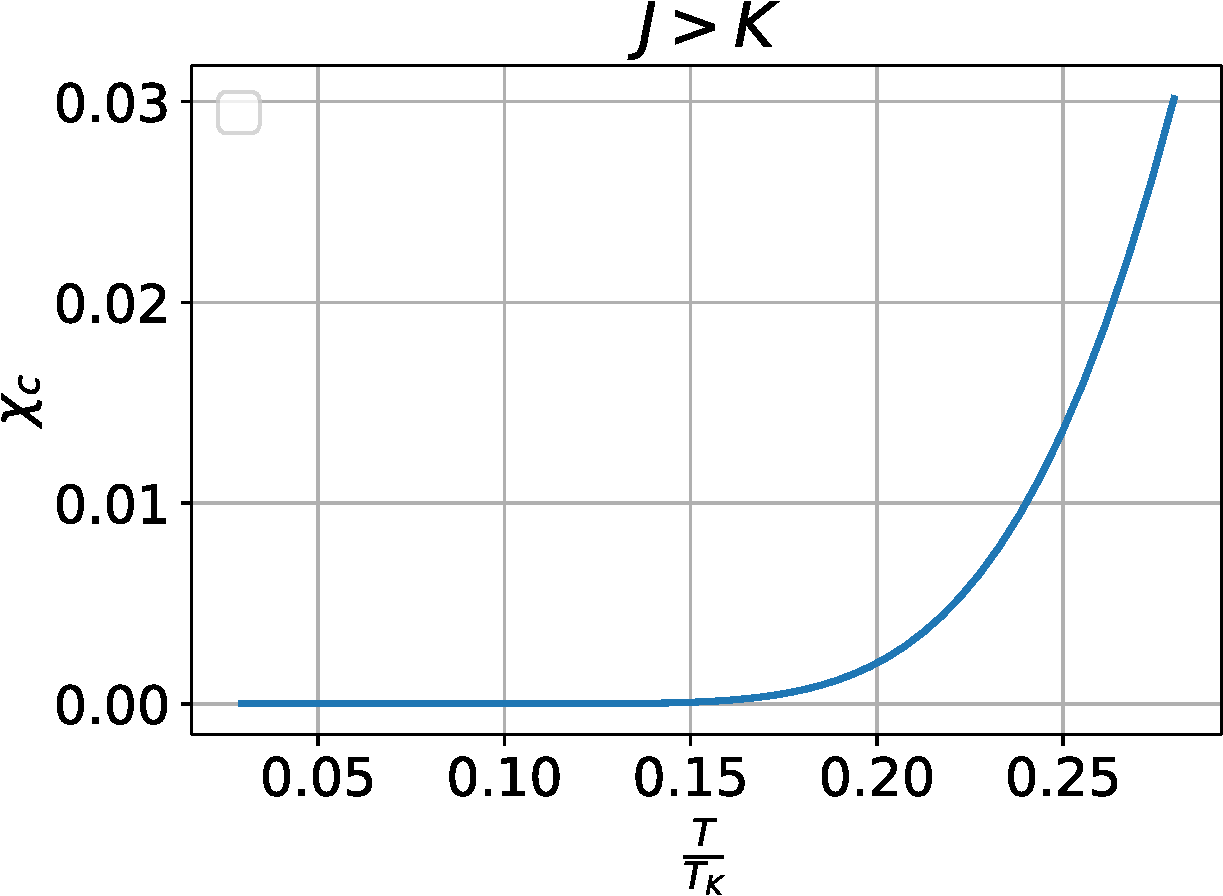
\includegraphics[width=0.48\textwidth]{figures/chi_c.pdf}
	\hspace*{25pt}
	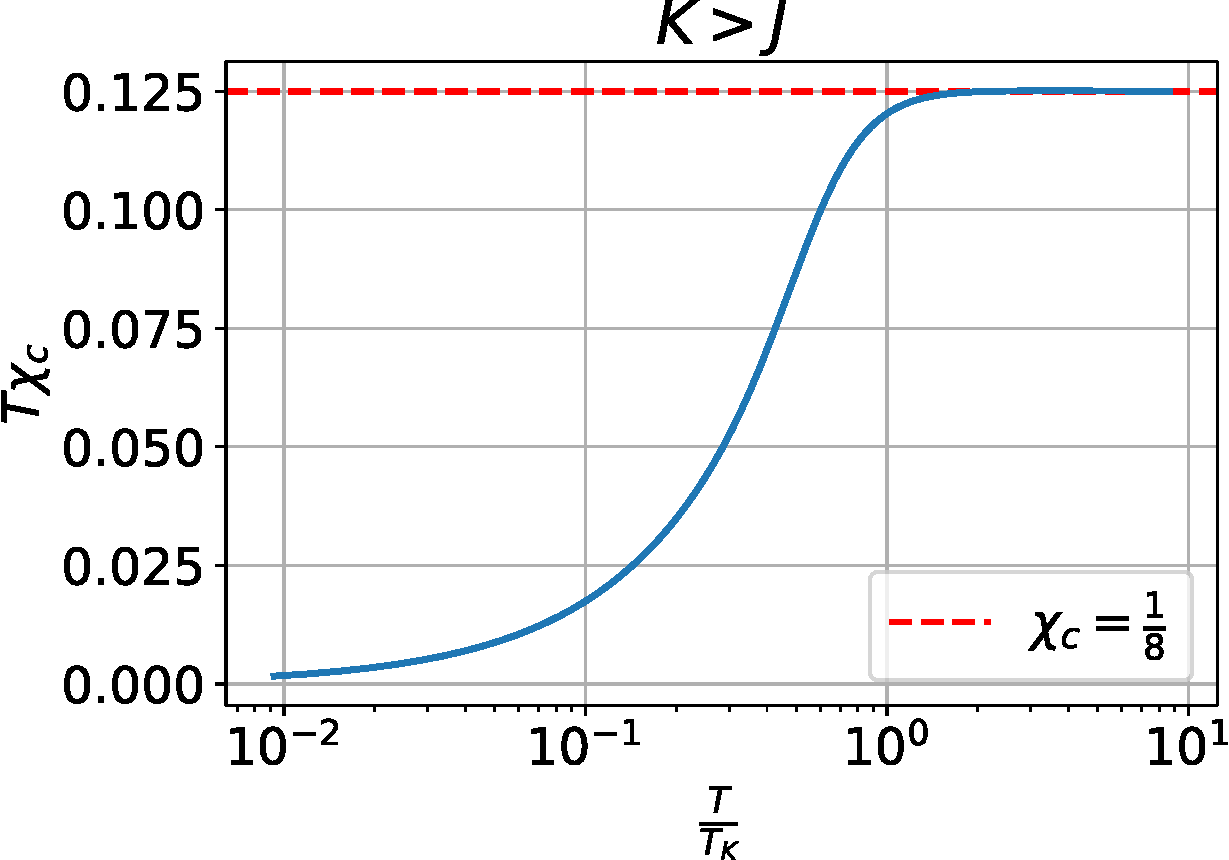
\includegraphics[width=0.48\textwidth]{figures/T_chi_c.pdf}
\end{center}
\large{\(
\left(\chi_c\times T\right)\left(T \to 0\right)\big\vert_{K>J} = \frac{1}{2k} \quad\quad\quad \left(\chi_c\times T\right)\left(T \to 0\right)\big\vert_{J>K} = 0 \quad\quad\quad \chi \left( T \to \infty \right) = \frac{1}{8}\)}

\footcite{taraphder,charge-kondo-Zitko}
\end{frame}

\begin{frame}[noframenumbering]{Results: Impurity Spectral Function}
	\(\mathcal{A(\omega)} = -\frac{1}{\pi}\text{Im }\left[G_{d d}^\sigma\left( \omega \right) \right]\) \hspace*{\fill} \(G_{d d}^\sigma\left(t\right) = -i\theta(t)\left<\left\{ c_{d\sigma}(t), c^\dagger_{d\sigma} \right\}\right>\)
\begin{center}
	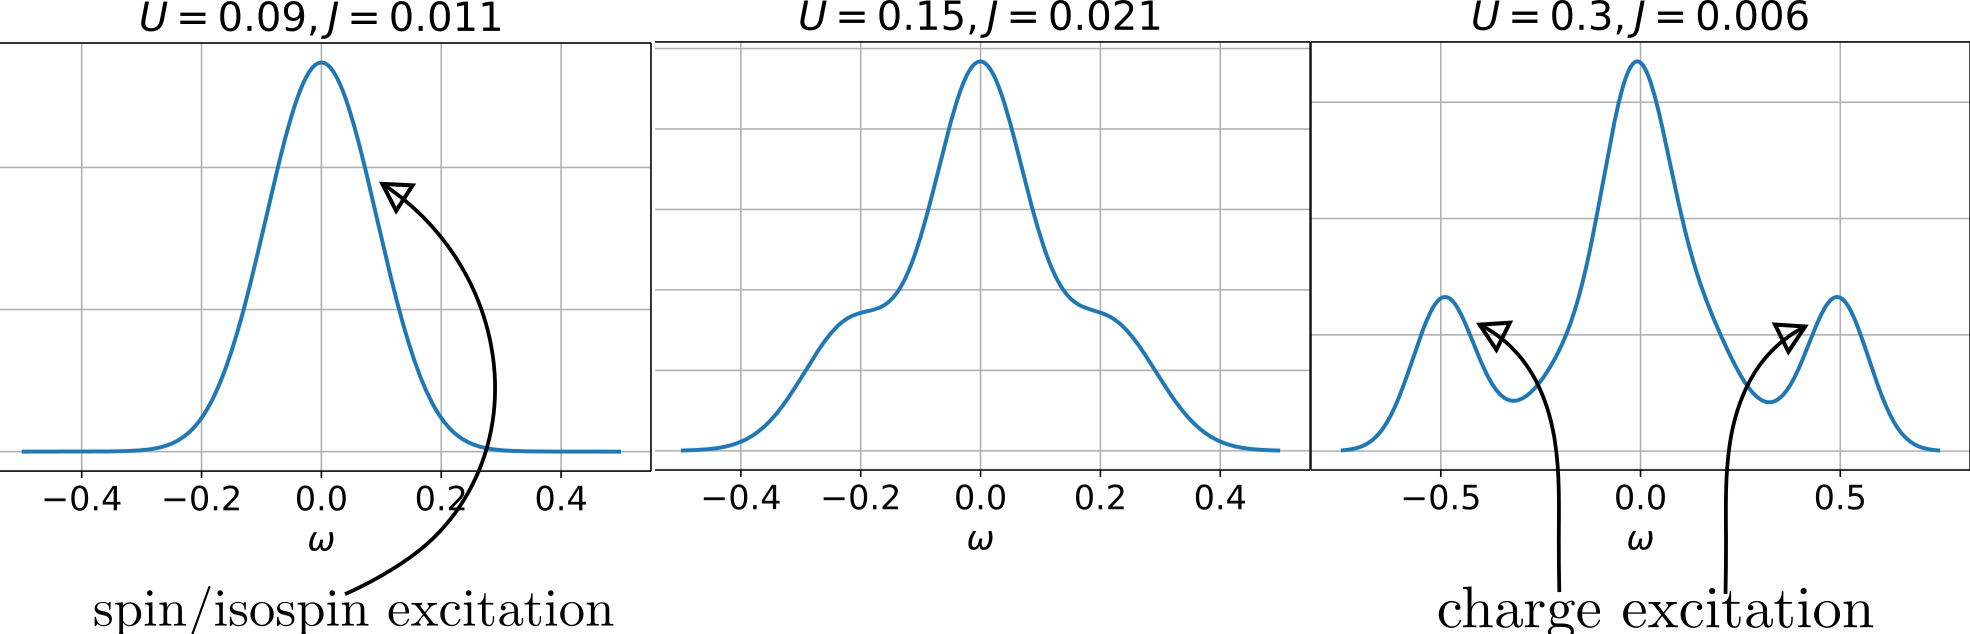
\includegraphics[width=\textwidth]{figures/spec_func_merged_2.png}
\end{center}
\footcite{hewson,bulla_costi_nrg}
\end{frame}

\begin{frame}[noframenumbering]{Results: Spectral Function Renormalization}
	\(\mathcal{A(\omega)} = -\frac{1}{\pi}\text{Im }\left[G_{d d}^\sigma\left( \omega \right) \right]\) \hspace*{\fill} \(G_{d d}^\sigma\left(t\right) = -i\theta(t)\left<\left\{ c_{d\sigma}(t), c^\dagger_{d\sigma} \right\}\right>\)
\begin{center}
	\includegraphics[width=0.47\textwidth]{figures/spec_func_journey_one_marked.pdf}\hspace*{\fill}\includegraphics[width=0.45\textwidth]{figures/spec_func_journey_three_marked.pdf}
\end{center}
\end{frame}

\begin{frame}[noframenumbering]{Results: Kondo Cloud Hamiltonian}
	\vspace*{-10pt}
	\[H^*(\text{d, cloud}) \xrightarrow{\text{solve for bath Hamiltonian}} H^*_\text{cloud}\] 
	\[H^*_\text{cloud} = \overbrace{H^*_0}^\text{kinetic energy} + \overbrace{\sum_{kk^\prime\sigma\sigma^\prime}f_{kk^\prime}\hat n_{k\sigma}\hat n_{k^\prime\sigma^\prime}}^\text{Fermi liquid-type interaction} + \overbrace{\sum_{kk^\prime qq^\prime}F_{kk^\prime qq^\prime}c^\dagger_{k \uparrow}c^\dagger_{k^\prime \downarrow} c_{q \uparrow}c_{q^\prime \downarrow}}^\text{non-Fermi liquid-type interaction}\]
\begin{figure}[htpb]
	\centering
	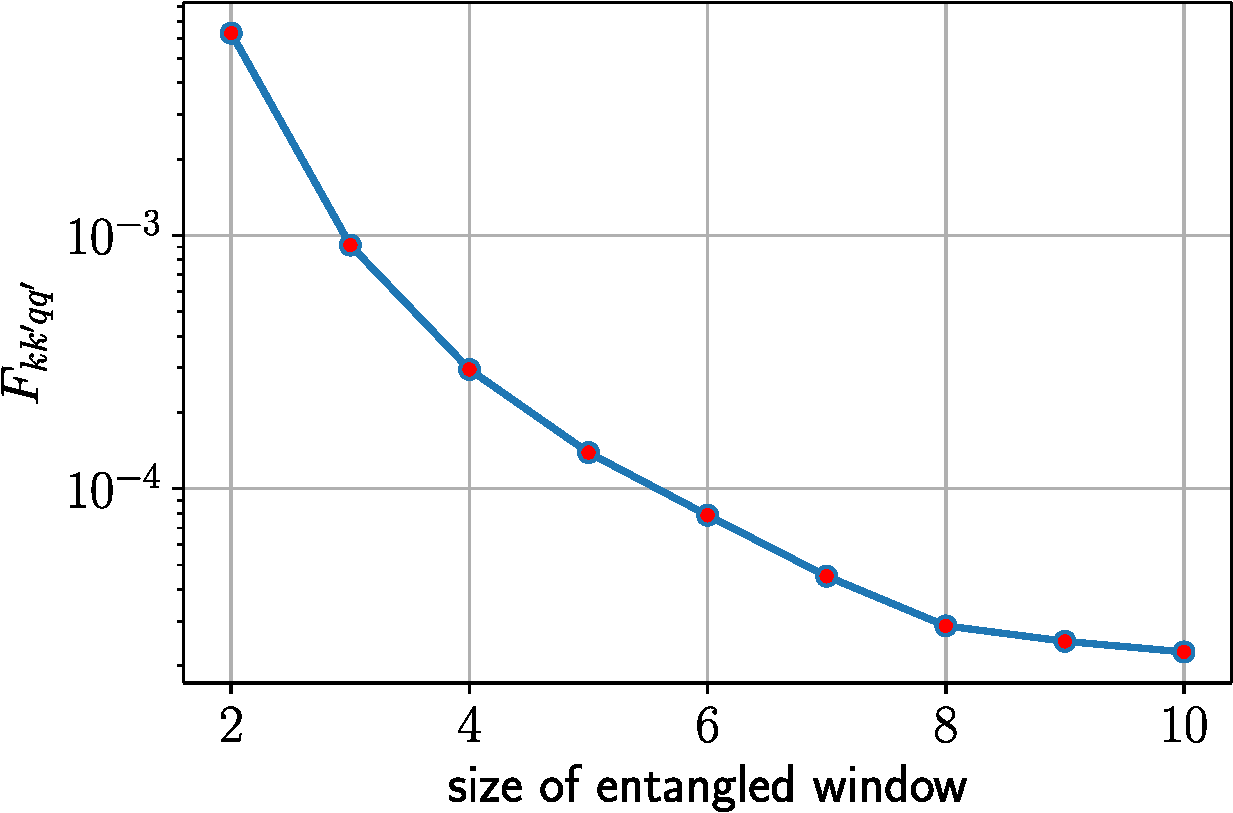
\includegraphics[width=0.45\textwidth]{figures/Fkkqq.pdf}
\end{figure}
\end{frame}

\begin{frame}[noframenumbering]{Results: Reverse RG: Overview}
	\vspace*{\fill}
	\begin{figure}[htpb]
		\centering
		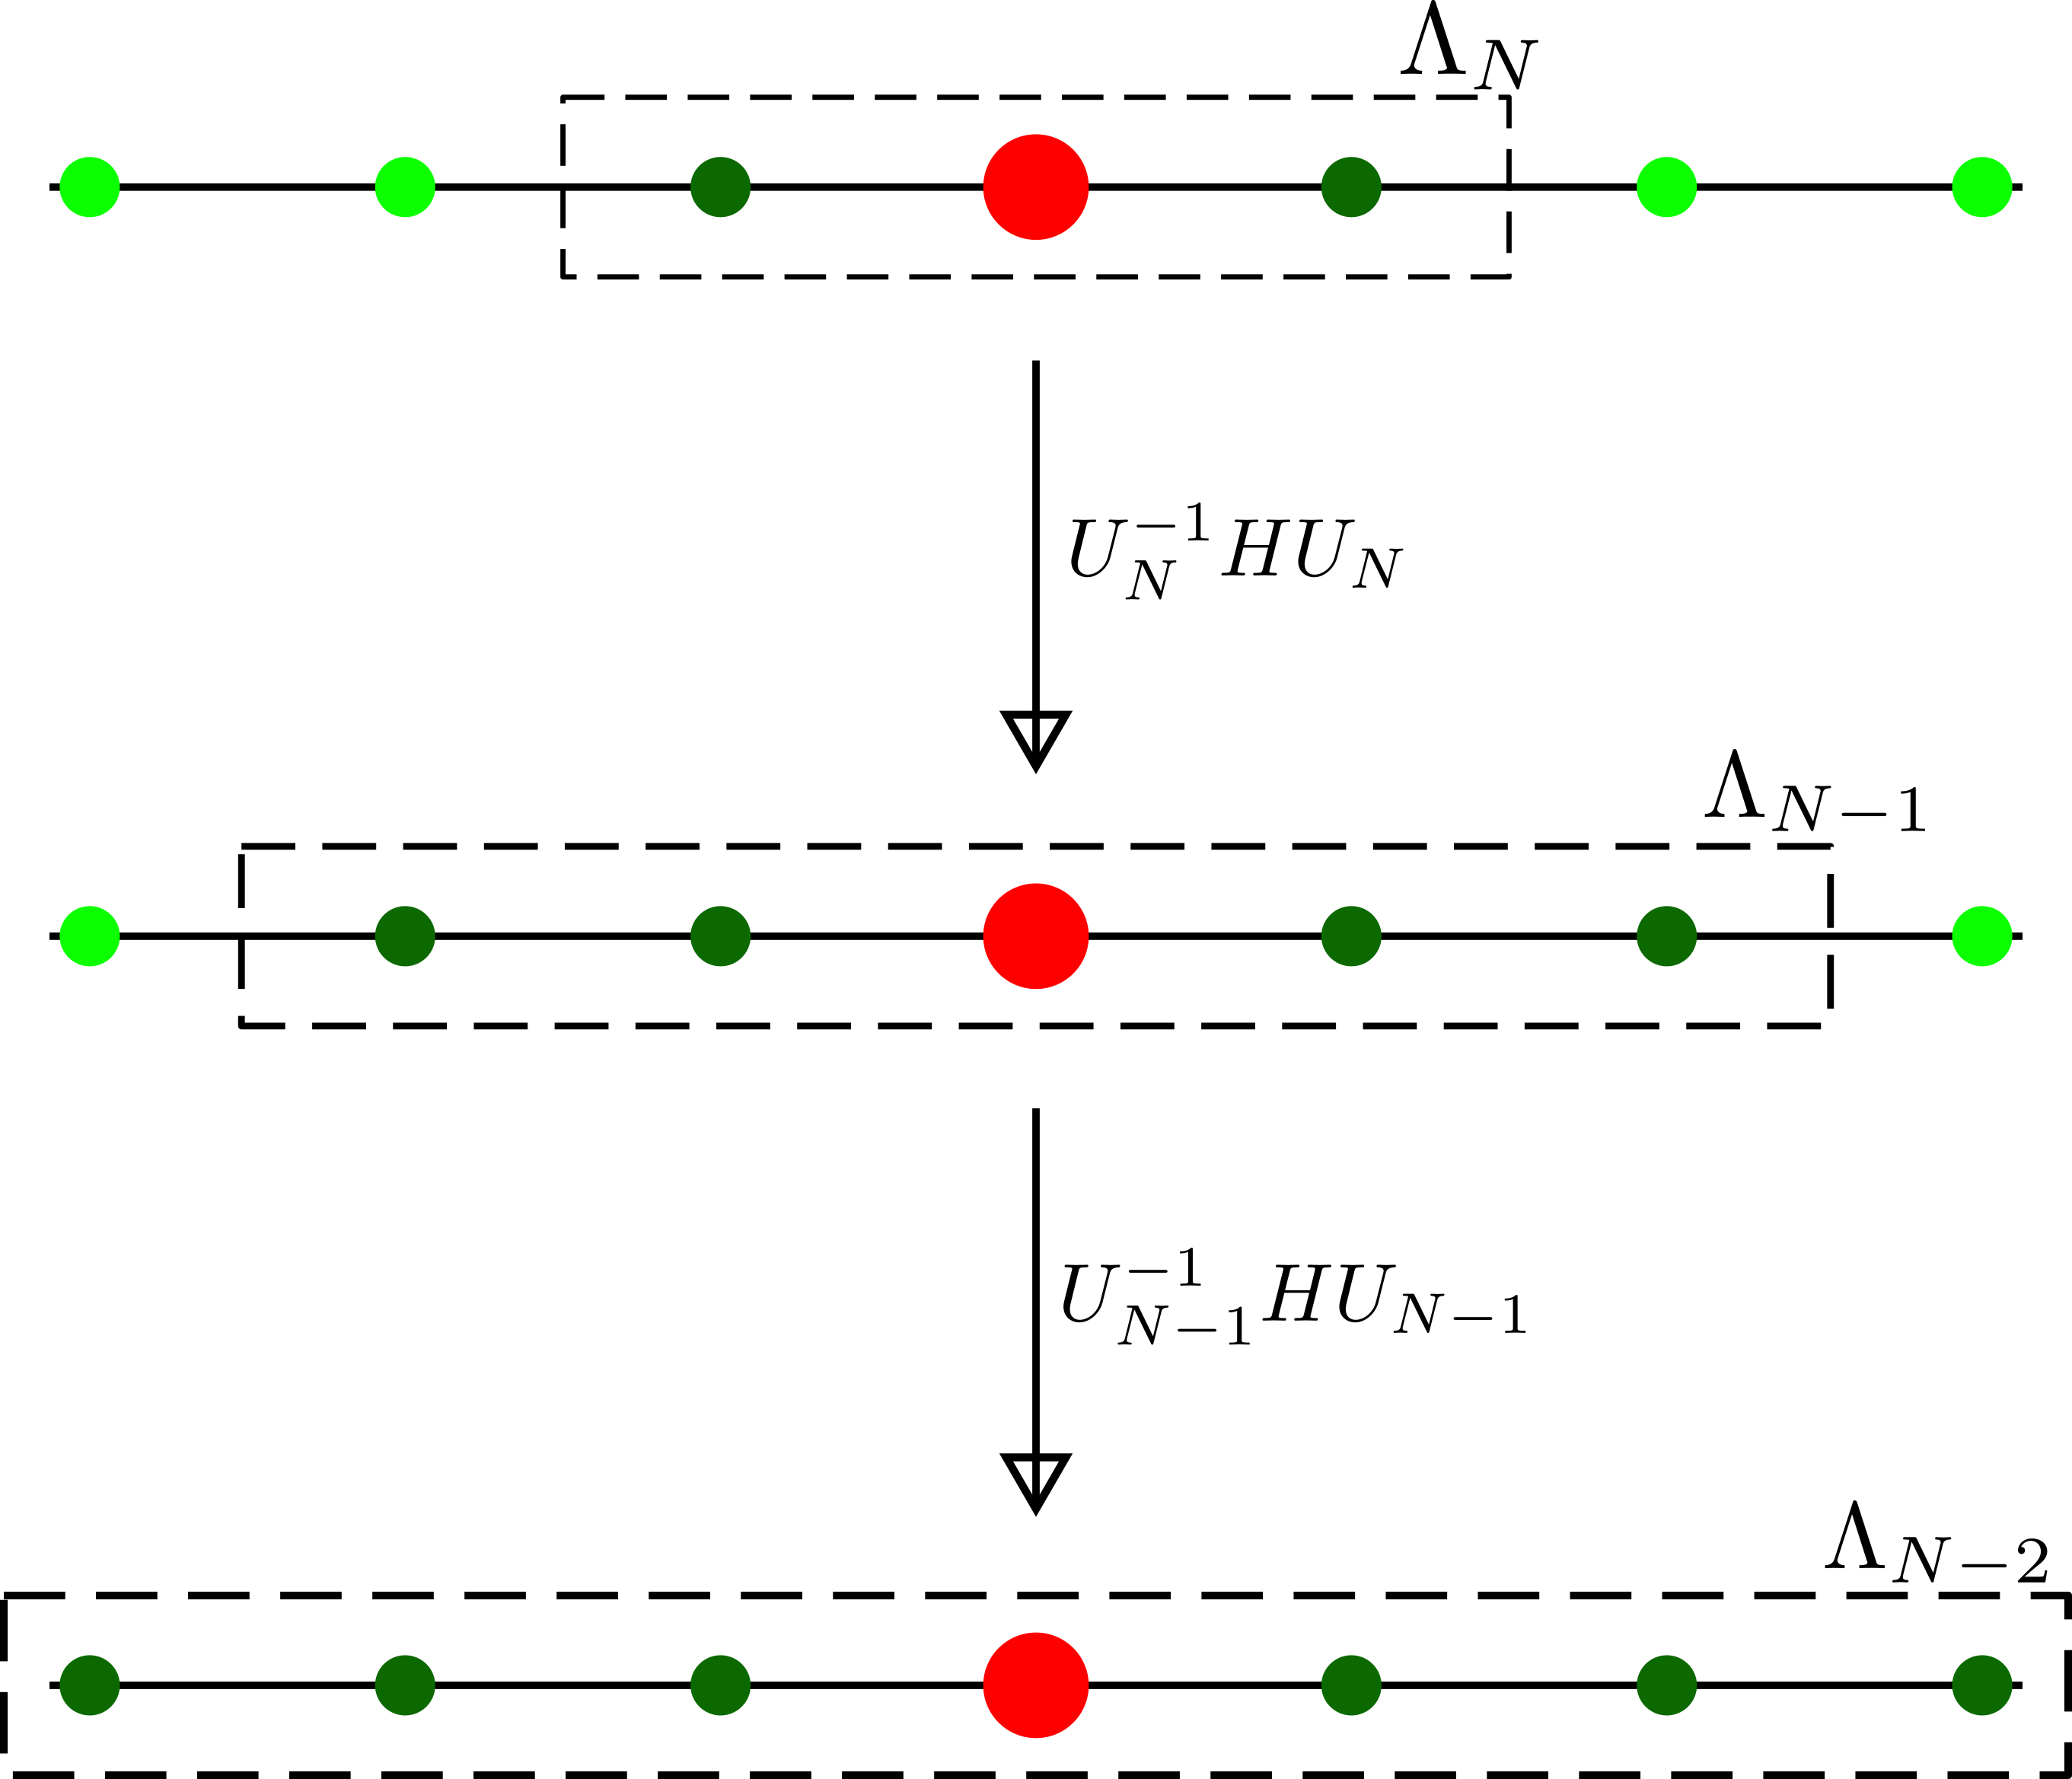
\includegraphics[width=0.5\textwidth]{figures/reverse-rg.png}
		\hspace*{\fill}
		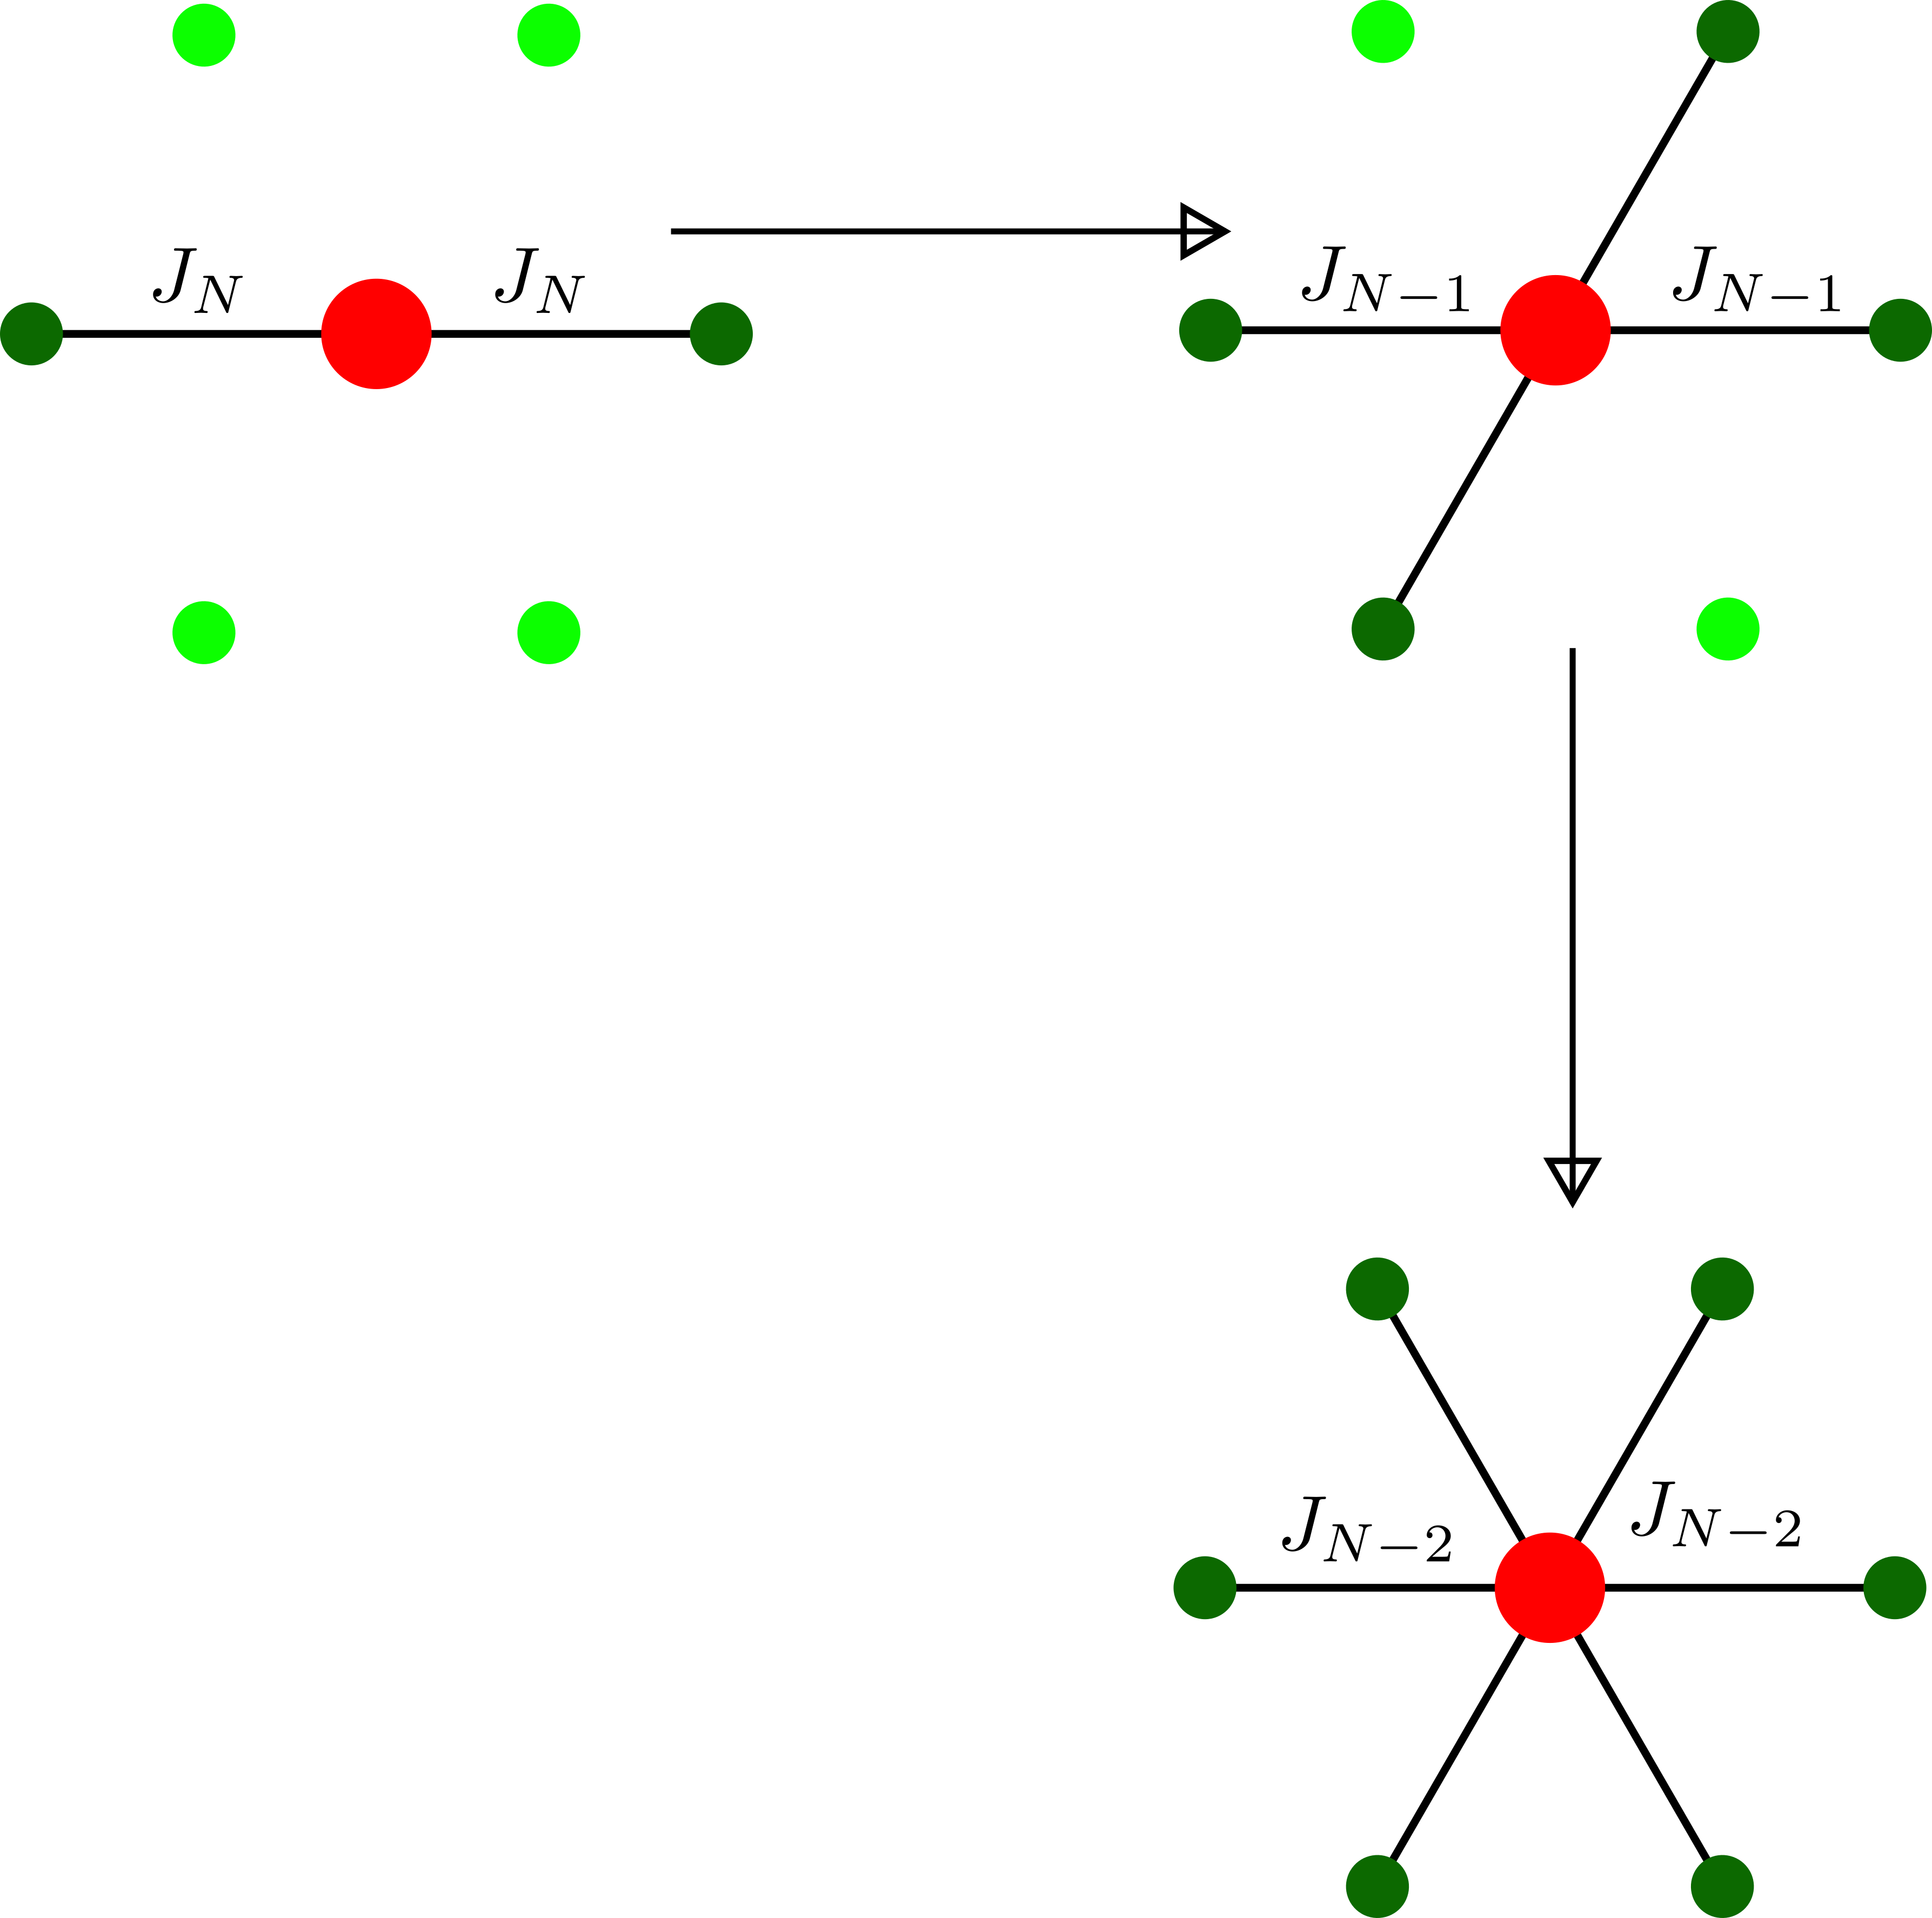
\includegraphics[width=0.45\textwidth]{figures/rev-rg-bonds-diag.png}
	\end{figure}
	\vspace*{\fill}
\footcite{am_thesis}
\end{frame}

\begin{frame}[noframenumbering]{Results: Reverse RG: Mutual Information}
	\hspace*{\fill}	\(I(A:B) = S_A + S_B - S_{AB}\)\hspace*{\fill}\(S_A = -\text{Tr }\left[\rho_A \ln \rho_A\right]\)\hspace*{\fill}
	\begin{figure}[htpb]
		\centering
		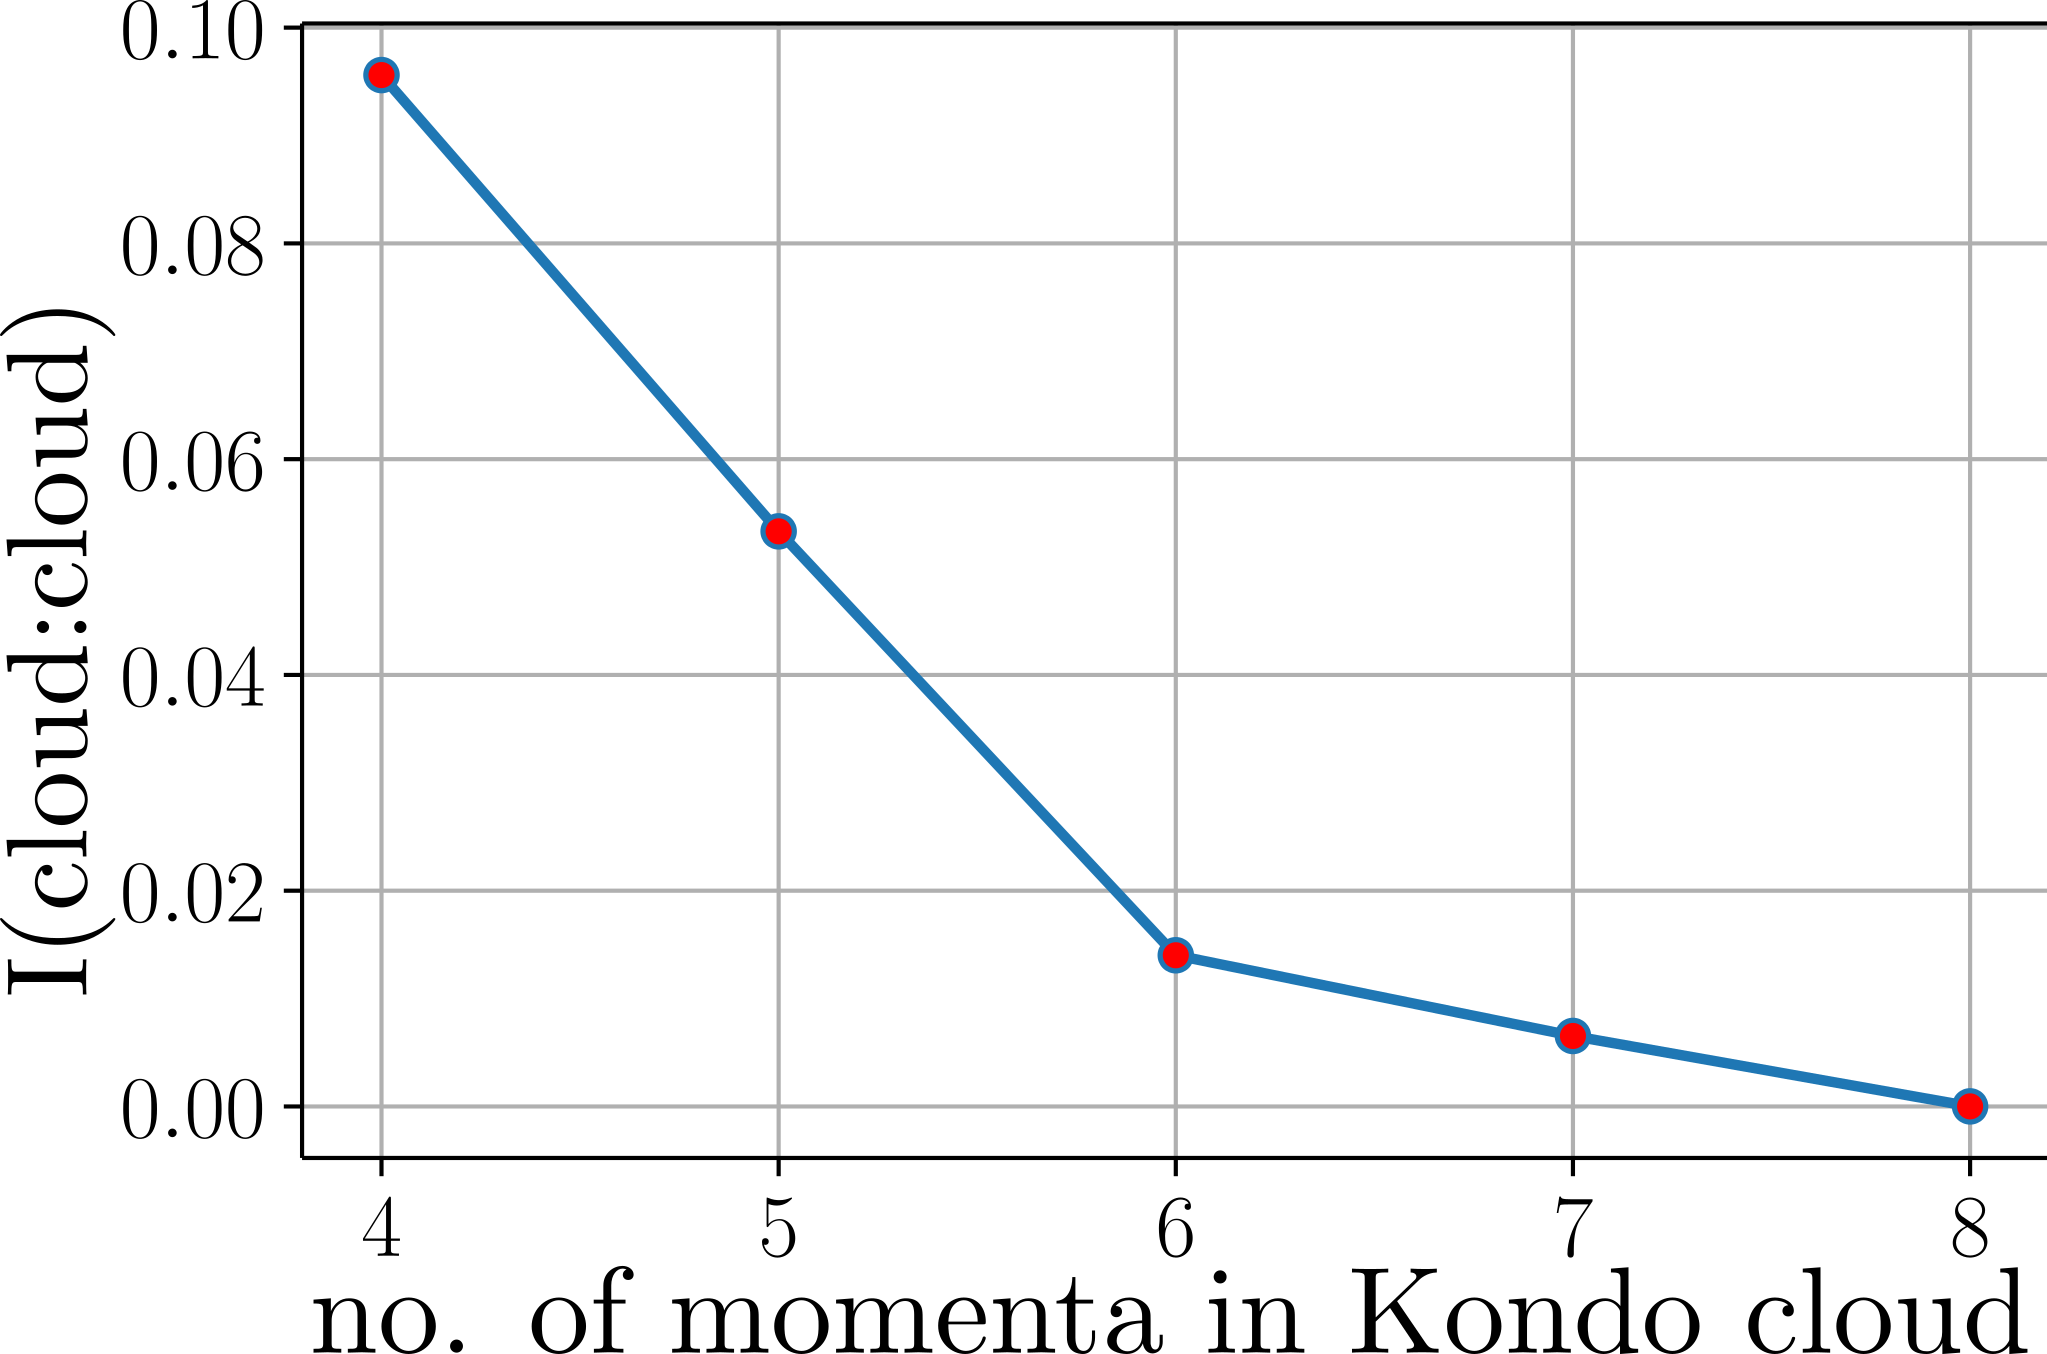
\includegraphics[width=0.45\textwidth]{figures/mutI_ee.png}\hspace*{\fill}
		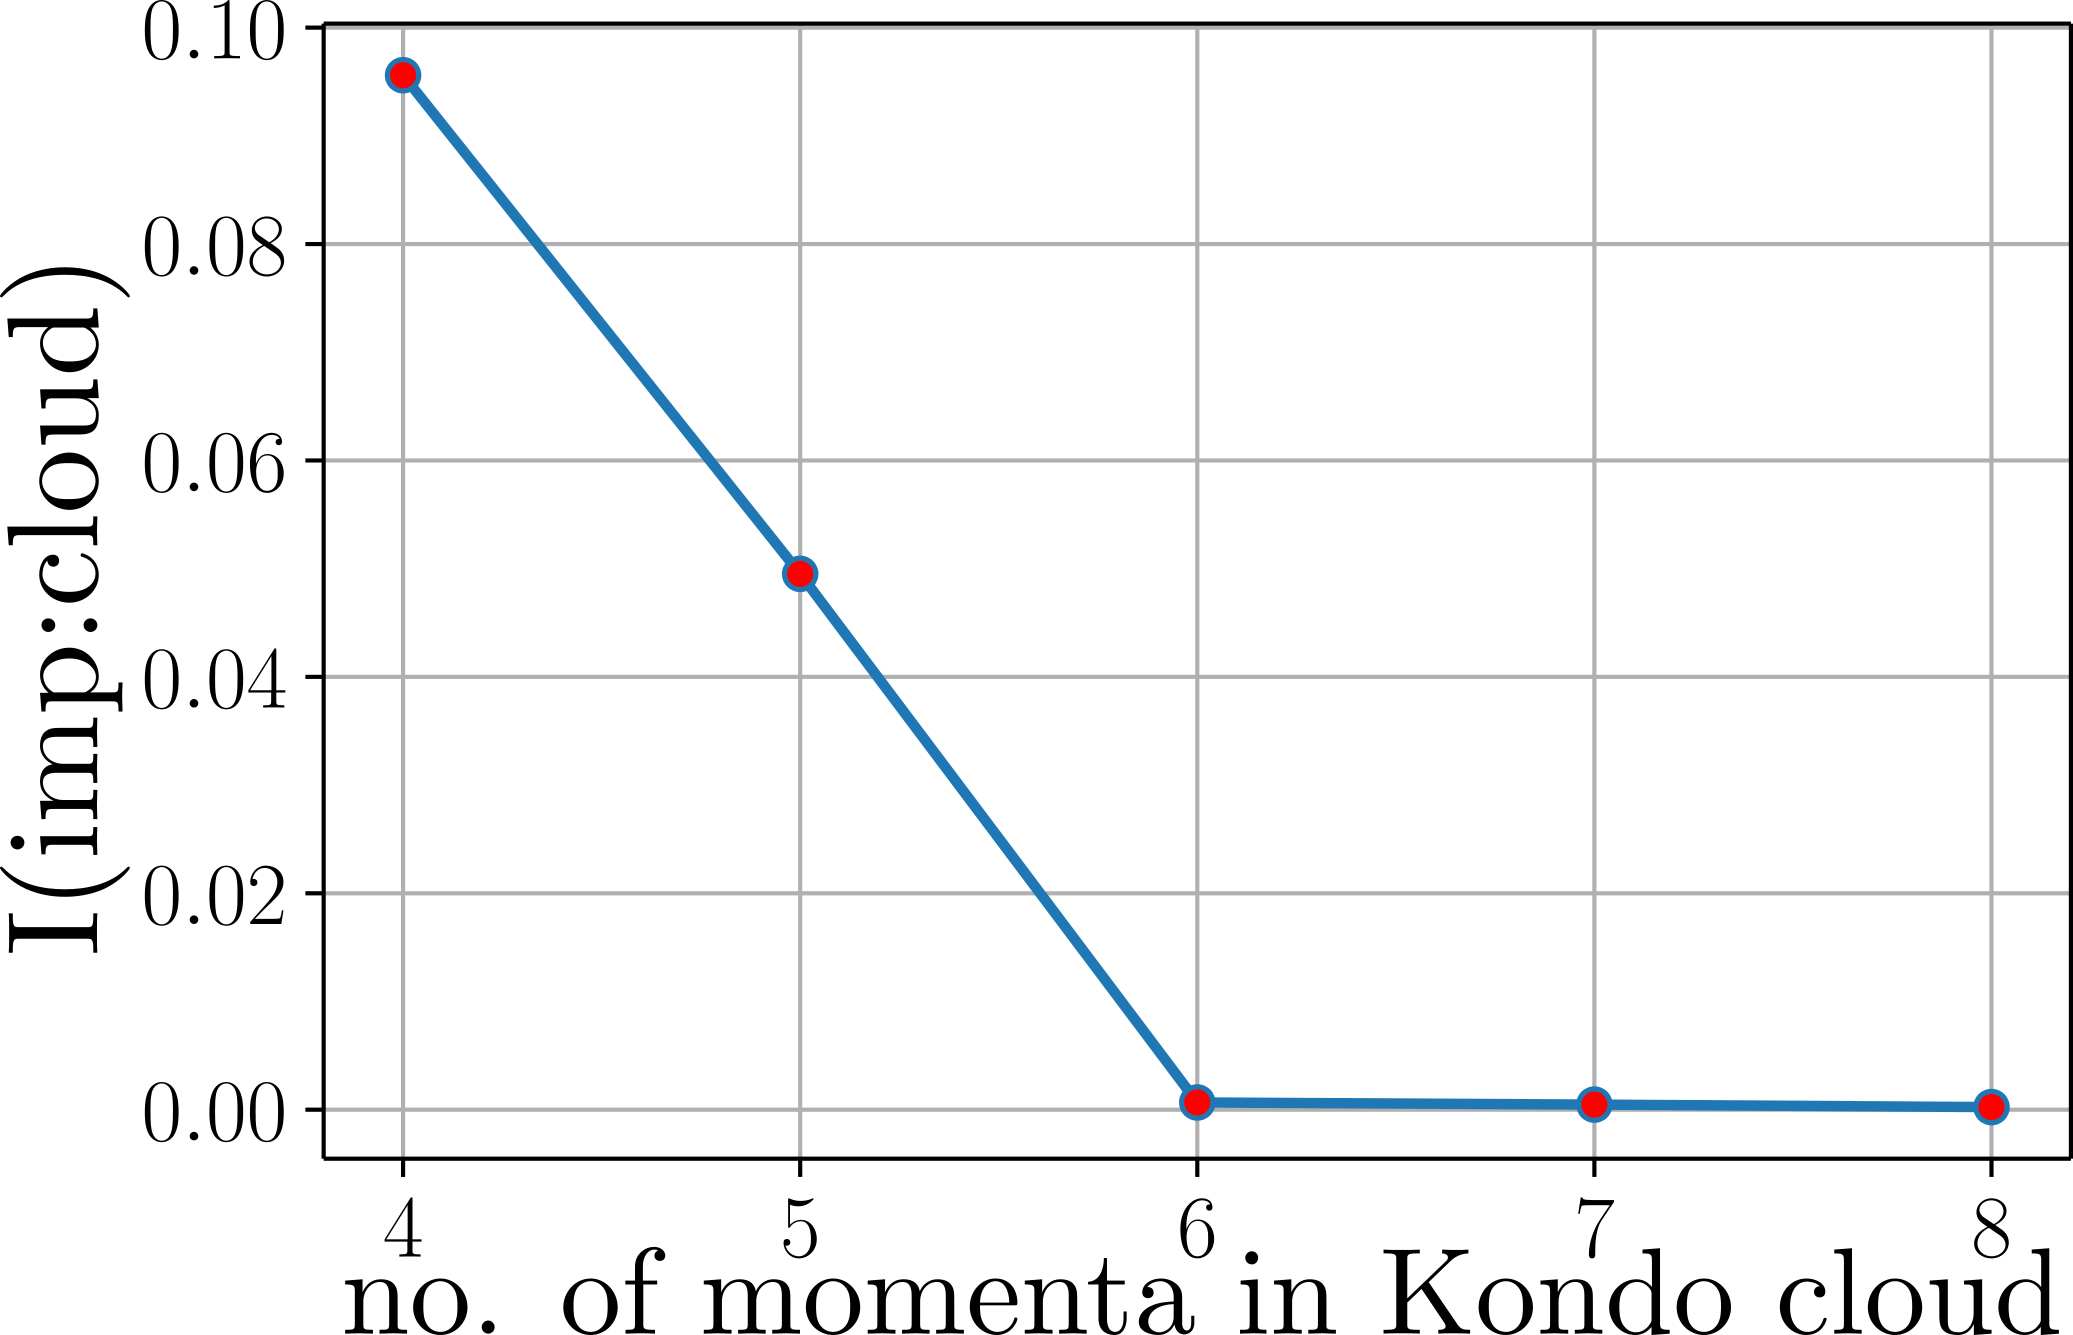
\includegraphics[width=0.45\textwidth]{figures/mutI_ed.png}
	\end{figure}
\end{frame}


\begin{frame}[noframenumbering]{Results: Reverse RG: Correlations}
	\begin{figure}[htpb]
		\centering
		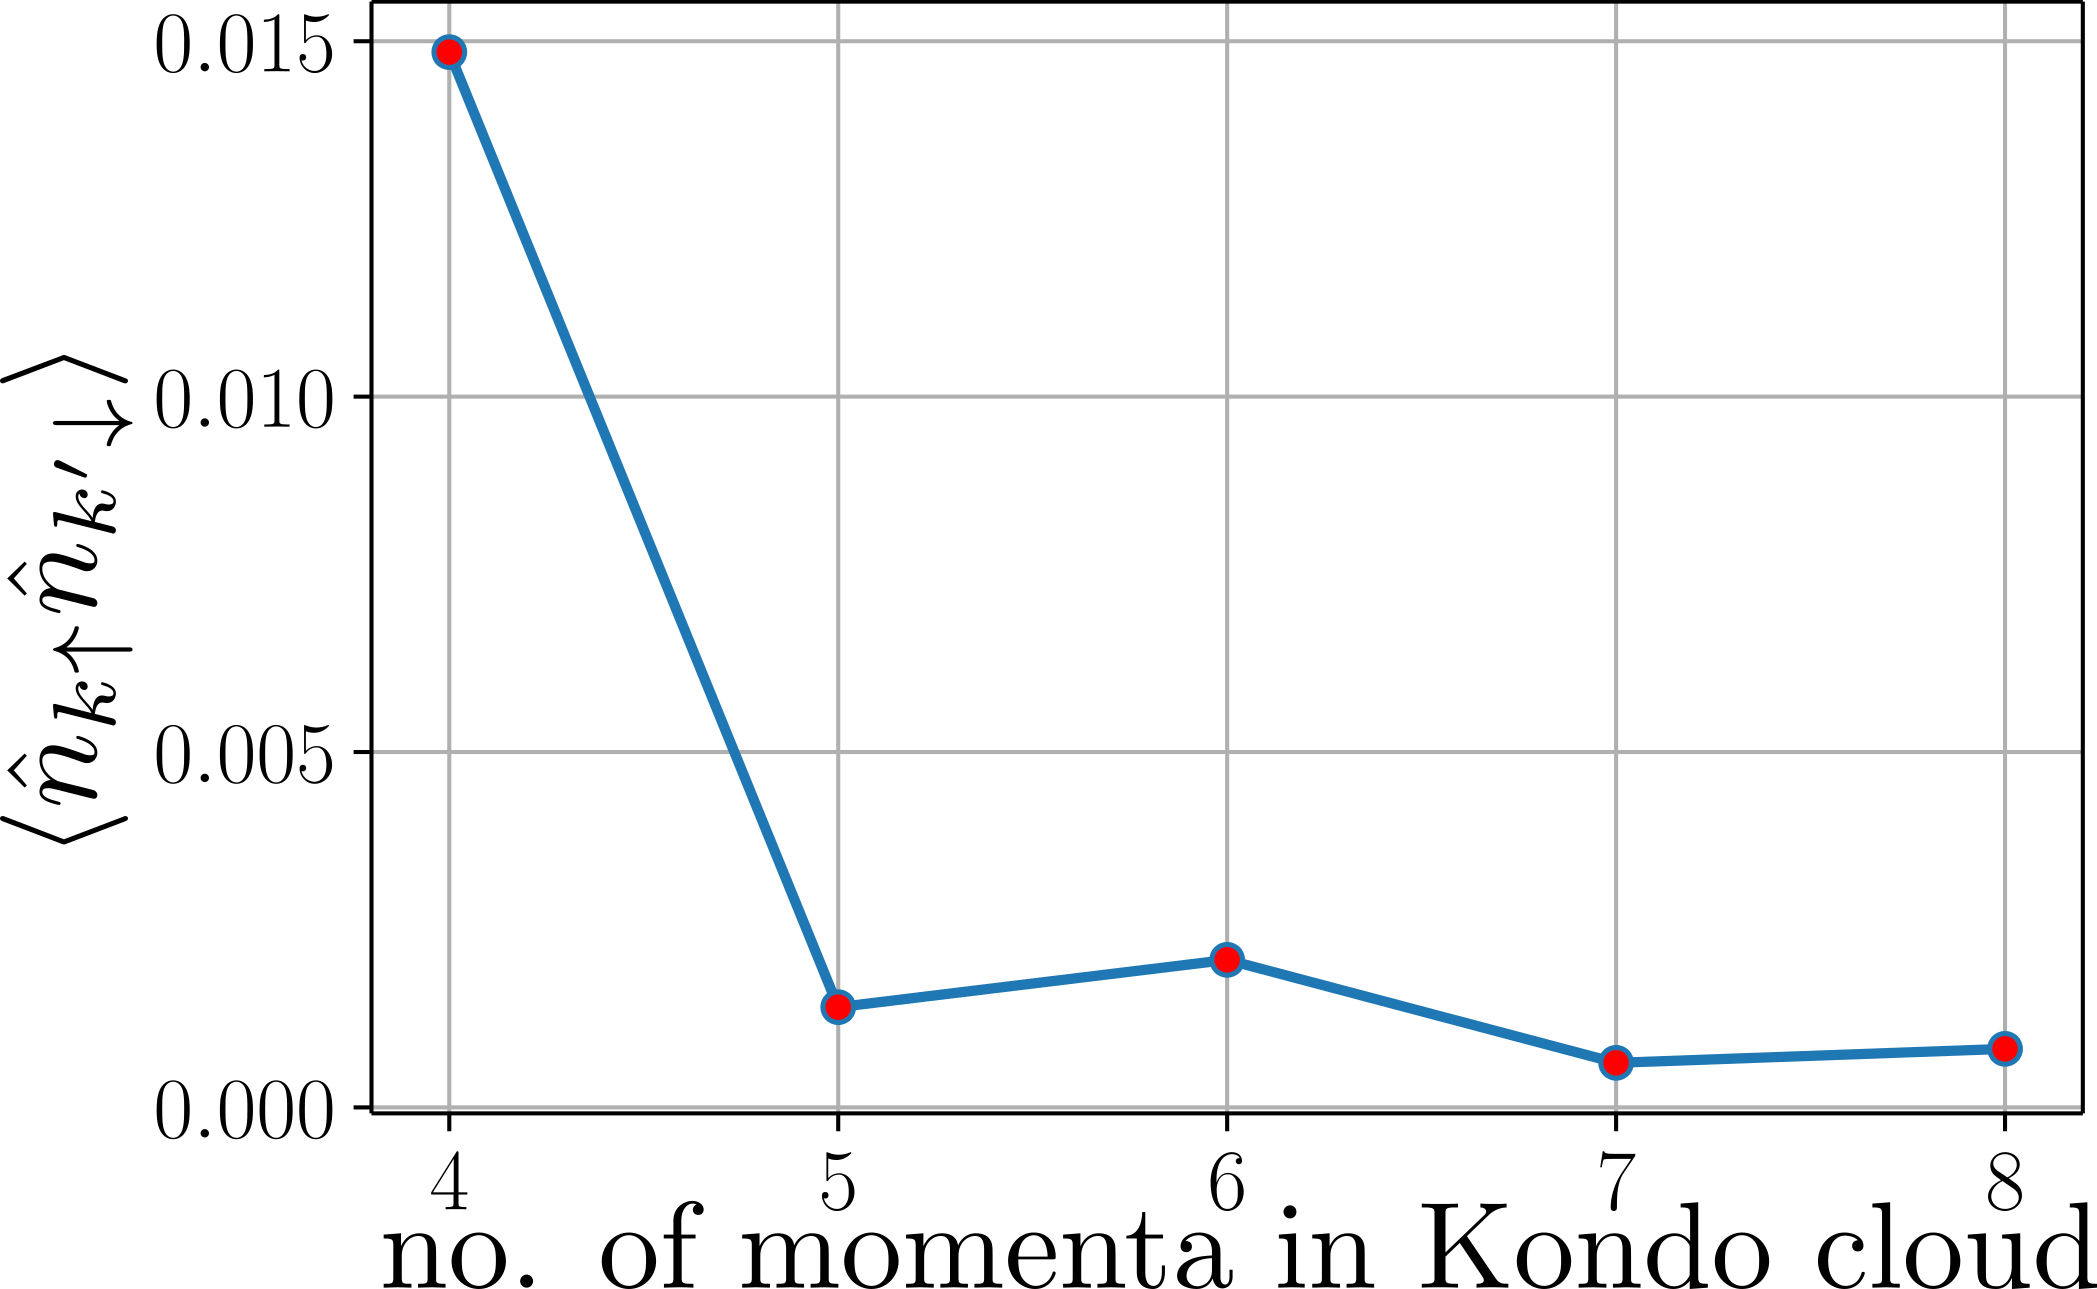
\includegraphics[width=0.45\textwidth]{figures/corr_diag.png}\hspace*{\fill}
		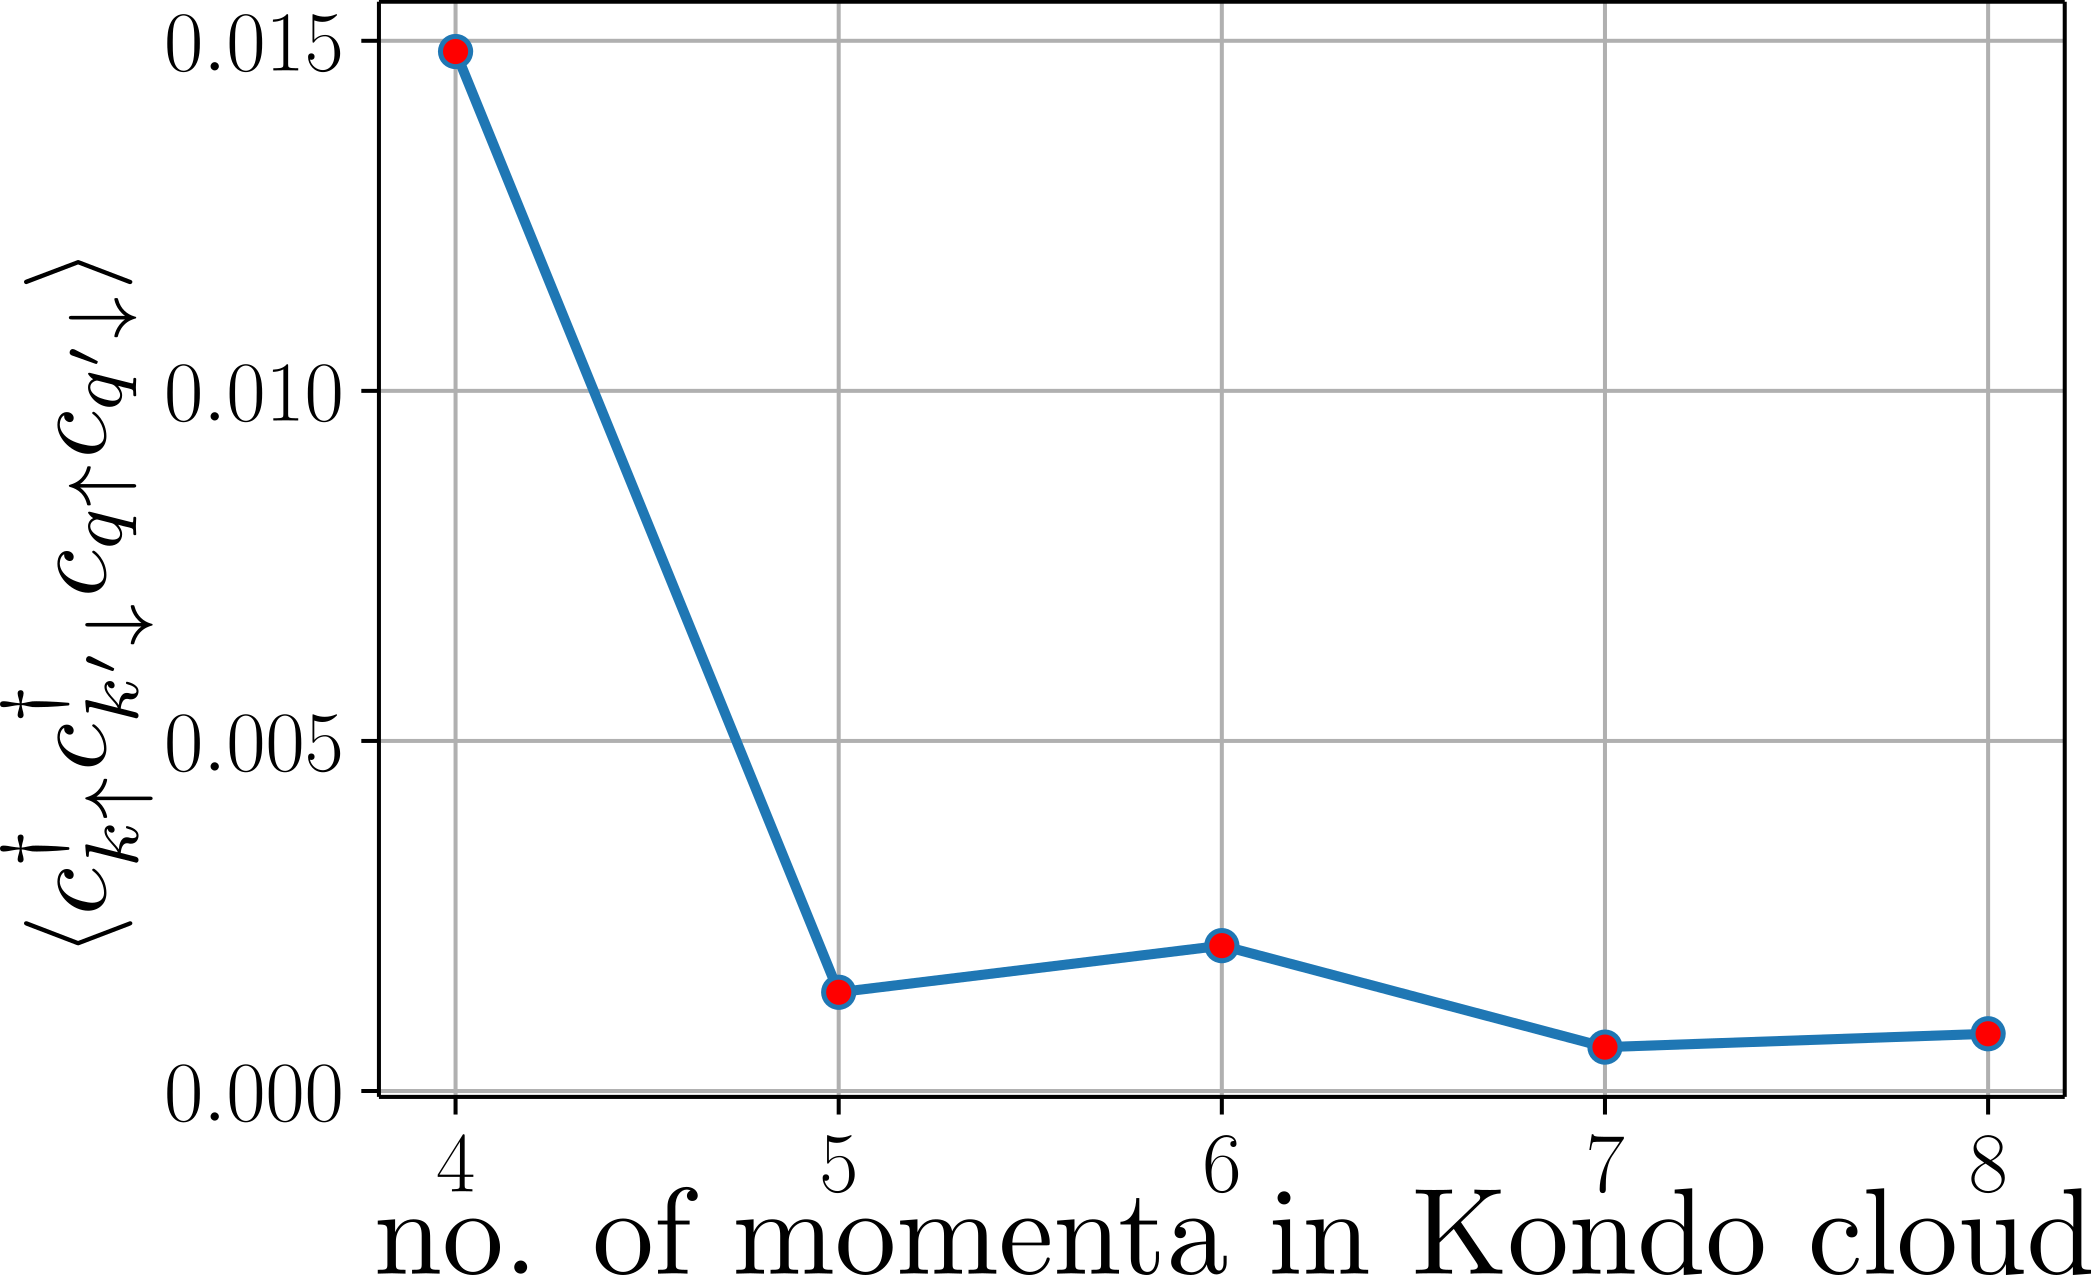
\includegraphics[width=0.45\textwidth]{figures/corr_od.png}
	\end{figure}
\end{frame}

\begin{frame}[noframenumbering]{Results: Luttinger's Theorem}
	\hspace*{\fill}	{\Large \(\overbrace{N}^{\text{total no. of}\atop{\text{ particles}}} = \overbrace{P_{\text{Det }G_d}(\Gamma_<) + \frac{1}{2}P_{\text{Det }G_d}(\Gamma_0)}^{\text{no. of poles of}\atop{\text{imp. Greens func.}}} + \overbrace{V_L}^{\text{no. of poles of}\atop{\text{cbath Greens func}}}\)}\hspace*{\fill}
\begin{equation*}\begin{aligned}
	P_X(C) &\equiv \frac{1}{2\pi i}\oint_C dz \frac{\partial{\ln X}}{\partial{z}} &&=\text{no. of poles of } X \text{ enclosed by curve }C \\
	       &= \frac{1}{2\pi i}\oint_{C(X)} \frac{dX}{X} &&= \text{winding number of } X \text{ around }X(C)
\end{aligned}\end{equation*}
\begin{minipage}{0.4\textwidth}
	\begin{figure}[htpb]
		\centering
		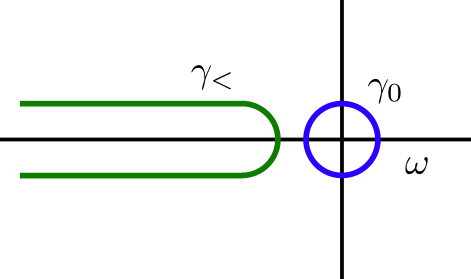
\includegraphics[width=0.9\textwidth]{figures/contours.png}
	\end{figure}
\end{minipage}
\hspace*{0.15\textwidth}
\begin{minipage}{0.4\textwidth}
	\begin{figure}[htpb]
		\centering
		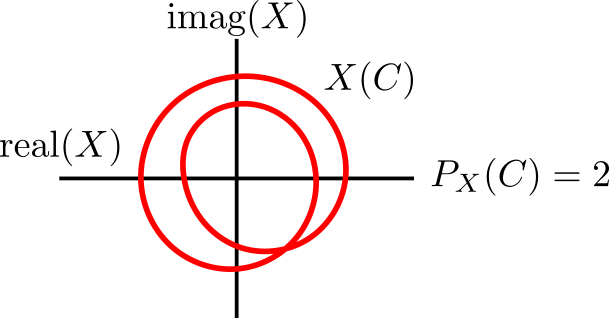
\includegraphics[width=0.9\textwidth]{figures/wind_num.png}
	\end{figure}
\end{minipage}
\footcite{seki}
\end{frame}

\begin{frame}[noframenumbering]{Results: Luttinger's Theorem}
\begin{minipage}{0.6\textwidth}
\begin{figure}[htpb]
	\centering
	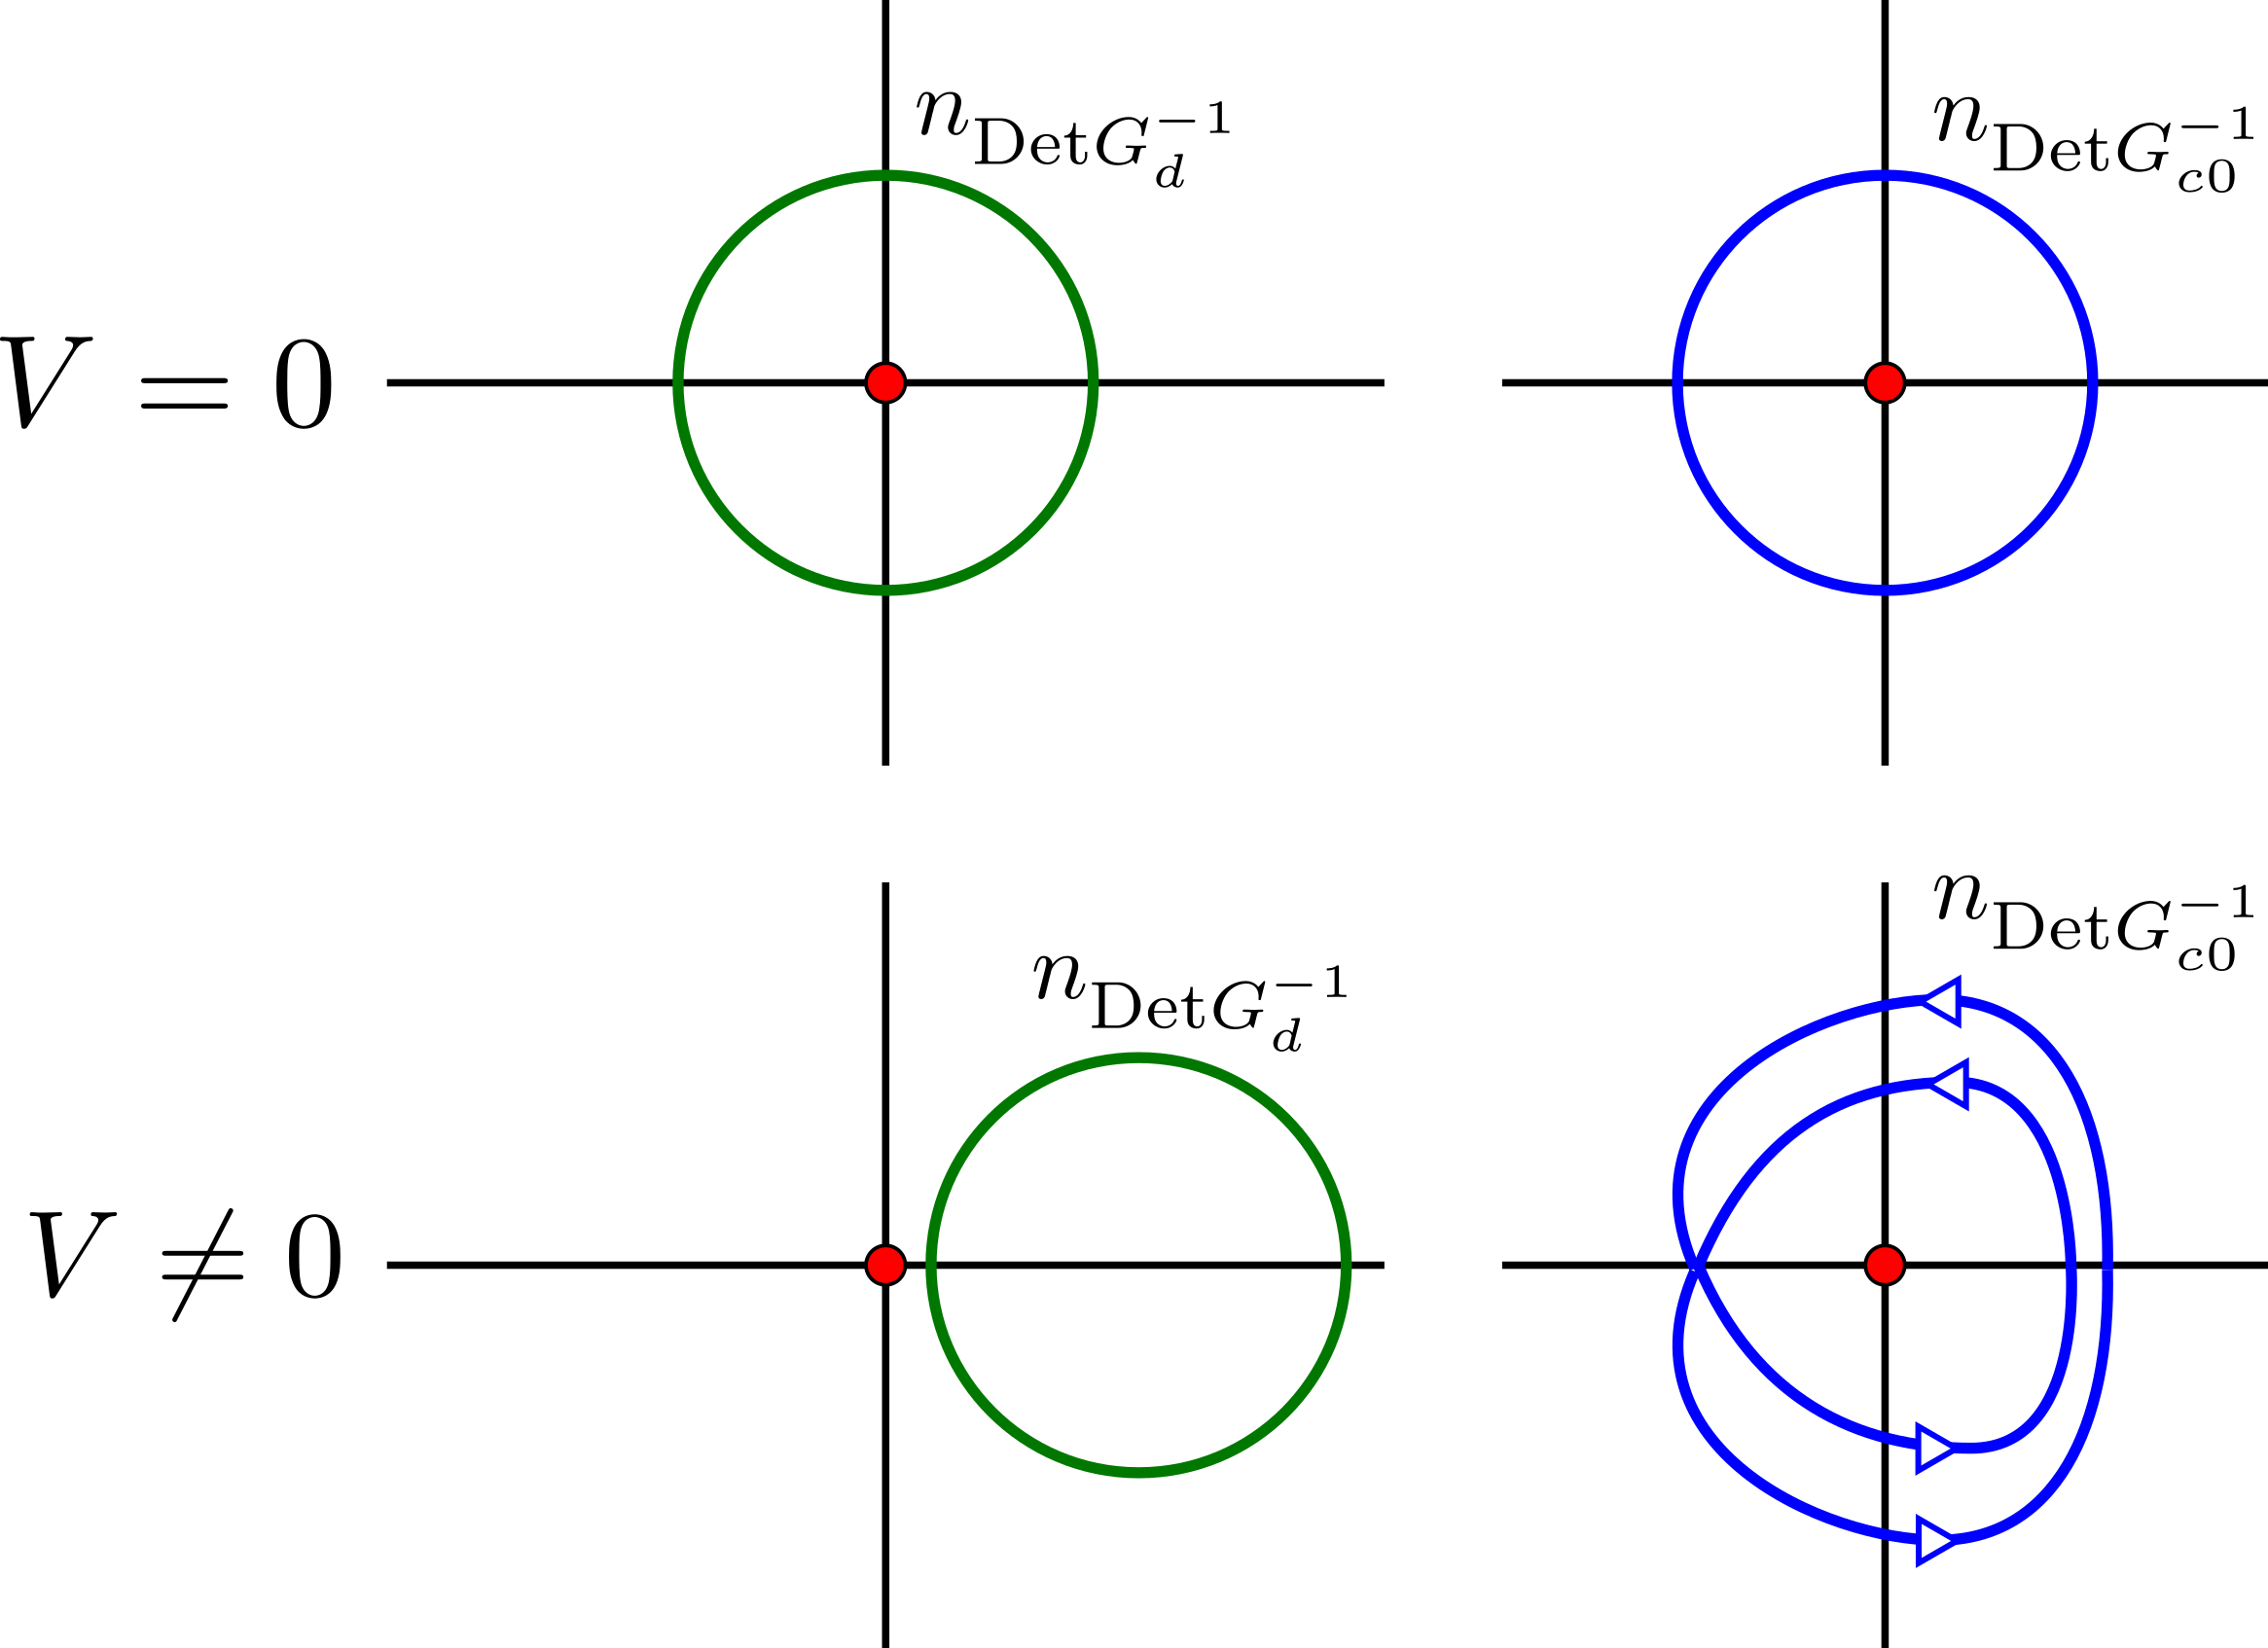
\includegraphics[width=0.75\textwidth]{figures/luttinger_top_change.png}
\end{figure}
\end{minipage}
\begin{minipage}{0.39\textwidth}
	\vspace*{5pt}
	{\large \[n_{\text{Det }G_d^{-1}} = 1\]
	\vspace*{45pt}
	\[n_{\text{Det }G_d^{-1}} = 0\]}
\end{minipage}
\vspace*{10pt}
\begin{center}
{ \LARGE \(V_L = V_L^0 + 1\)}
\end{center}
\footcite{martin}
\end{frame}

\begin{frame}[noframenumbering]{Results: Local Fermi Liquid}
	\[H^* = \overbrace{J^* \vec{S_d}\cdot\vec{s} + K^* \vec{C_d}\cdot\vec{c} + V^* \left( c^\dagger_{d\sigma}c_{0\sigma} + \text{h.c.} \right)}^\text{solve exactly} + \overbrace{t\sum_{\left<i,j \right>}c^\dagger_{i\sigma}c_{j\sigma}}^\text{treat as perturbation}\]
	\hspace*{0.5\textwidth}$\Bigg\downarrow$ \(4^\text{th}\) fourth order pert.
	\[E_1^{(4)} = -\frac{16t^4}{3{J^*}^3}, E_2^{(4)} = -\frac{16t^4}{9{J^*}^3}\]
	\[H^* \sim J^* \vec{S_d}\cdot\vec{s} + K^* \vec{C_d}\cdot\vec{c} + V^* \left( c^\dagger_{d\sigma}c_{0\sigma} + \text{h.c.} \right) + \overbrace{\frac{t^4}{{J^*}^3} \hat n_{1 \uparrow}\hat n_{1 \downarrow}}^\text{local Fermi liquid}\]
	\[ \left< \hat n_{1 \uparrow}\hat n_{1 \downarrow}\right> \xrightarrow{\text{mean field}\atop \text{approximation}} \left<\hat n_{1 \uparrow}\right>\left< \hat n_{1 \downarrow}\right>\]

\vspace*{-10pt}
\footcite{nozieres}
\end{frame}

\begin{frame}[noframenumbering]{Results: Wilson Ratio (\(T=0\))}
	\begin{center}
	\scalebox{1.5}{
	$\epsilon_{k\sigma} = \epsilon_k^0 + \sum_q f_{kq}\left<n_{q\overline\sigma} \right>$}
\end{center}
\vspace*{\fill}
\begin{minipage}{0.45\textwidth}
\begin{itemize}
	\item \(f_{\uparrow\uparrow} =0\)
	\item \(\chi_c(T\to 0) =0\)
\end{itemize}
\end{minipage}
\begin{minipage}{0.2\textwidth}
	\scalebox{2}{$\longrightarrow$}
\end{minipage}
\begin{minipage}{0.33\textwidth}
\begin{itemize}
	\item \(C_v(T\to 0) = \rho_\text{imp}T\)
	\item \(\chi_s(T \to 0) = 2\rho_\text{imp}\)
\end{itemize}
\end{minipage}
\vspace*{\fill}
\begin{center}
	\scalebox{1.5}{
	$R = \frac{\chi_s}{\gamma} = 2$}
\end{center}
\footcite{hewsonp}
\end{frame}

\begin{frame}[noframenumbering]{Results: Relation between \(R\) and \(\Delta V_L\)}
	\begin{minipage}{0.43\textwidth}
		\begin{itemize}
			\item particle-hole symmetry
			\item strong-coupling fixed-point
			\item \(T=0\)
		\end{itemize}
	\end{minipage}
	\begin{minipage}{0.18\textwidth}
		\begin{center}
			\LARGE\(\longrightarrow\)
		\end{center}
	\end{minipage}
	\begin{minipage}{0.22\textwidth}
		\Large\(R = 1 + \sin^2 \delta(0)\)
	\end{minipage}
	\\[30pt]
	\begin{minipage}{0.43\textwidth}
		\begin{itemize}
			\item Friedel's sum rule 
			\item scattering theory arguments
		\end{itemize}
	\end{minipage}
	\begin{minipage}{0.18\textwidth}
		\begin{center}
			\LARGE\(\longrightarrow\)
		\end{center}
	\end{minipage}
	\begin{minipage}{0.25\textwidth}
		\Large\(\frac{1}{\pi}\delta(0) = \tilde N = \Delta V_L\)
	\end{minipage}
	\\[30pt]

	\begin{center}
		\Large\(R = 1 + \sin^2 \left( \pi \Delta V_L \right) \)\\[10pt]
		\Large\(\Delta V_L = 1 \longrightarrow R = 2 \)
	\end{center}

\end{frame}
% \only<1>{
% \begin{flalign*}
% 	\mathcal{H} = \overbrace{\sum_{k\sigma}\epsilon_k \hat n_{k\sigma} + \sum_{k\sigma}\left[V(k)c^\dagger_{k\sigma}c_{d\sigma} + \text{h.c.}\right] + \epsilon_d \sum_\sigma \hat n_{d\sigma} + U\hat n_{d\uparrow}\hat n_{d\downarrow}}^{SIAM}\\
%  + \underbrace{J \vec{S_d}\cdot \sum_{kq\alpha\beta}\vec{\sigma}_{\alpha,\beta}c^\dagger_{k\alpha}c_{q\beta}}_\text{spin-exchange}+ \underbrace{J \vec{C_d}\cdot \sum_{kq\alpha\beta}\vec{\sigma}_{\alpha,\beta}\psi^\dagger_{k\alpha}\psi_{q\beta}}_\text{isospin-exchange}
% \end{flalign*}
% }
% \only<2-3>{\Large{\textbf{RG Equations}}
% \only<2>{
% 	\vspace*{-15pt}
% 		\begin{equation*}\begin{aligned}\Delta U &= \left(U + \frac{1}{2}J\right)\sum_{|q|=\Lambda_n} \frac{|V(q)|^2}{(\omega - \epsilon_q - \frac{1}{2}U - \frac{1}{4}J)(\omega - \epsilon_q)}\\[5pt]
% 			\Delta V(q) &= -\frac{3}{4}J\sum_{|q|=\Lambda_n} \frac{V(q)}{\omega - \epsilon_q - \frac{1}{2}U - \frac{1}{4}J}\\[5pt]
% \Delta J &= -\frac{1}{4}J^2\sum_{|q|=\Lambda_n\atop{k<\Lambda_n}} \frac{1}{\omega - \epsilon_q - \frac{1}{2}U - \frac{1}{4}J}\end{aligned}\end{equation*}
% }
% \only<3>{
% 	\vspace*{25pt}
% \begin{itemize}
% 	\item Particle-hole symmetric
% 	\vspace*{10pt}
% 	\item Hermitian
% 	\vspace*{10pt}
% 	\item \(SU(2)\)-symmetric
% 	\vspace*{10pt}
% 	\item Reduce to Poor Man's scaling and Kondo 1-loop forms
% \end{itemize}
% }
% }
% \end{frame}

% \begin{frame}[noframenumbering]{Results (\(\pmb{J=0}\))}
% \vspace*{-10pt}
% \begin{figure}
% \def\svgwidth{\columnwidth}
% \centering
% \scalebox{1}{\input{lmflow.pdf_tex}}
% \end{figure}
% \only<1>{\vspace*{10pt}\centering 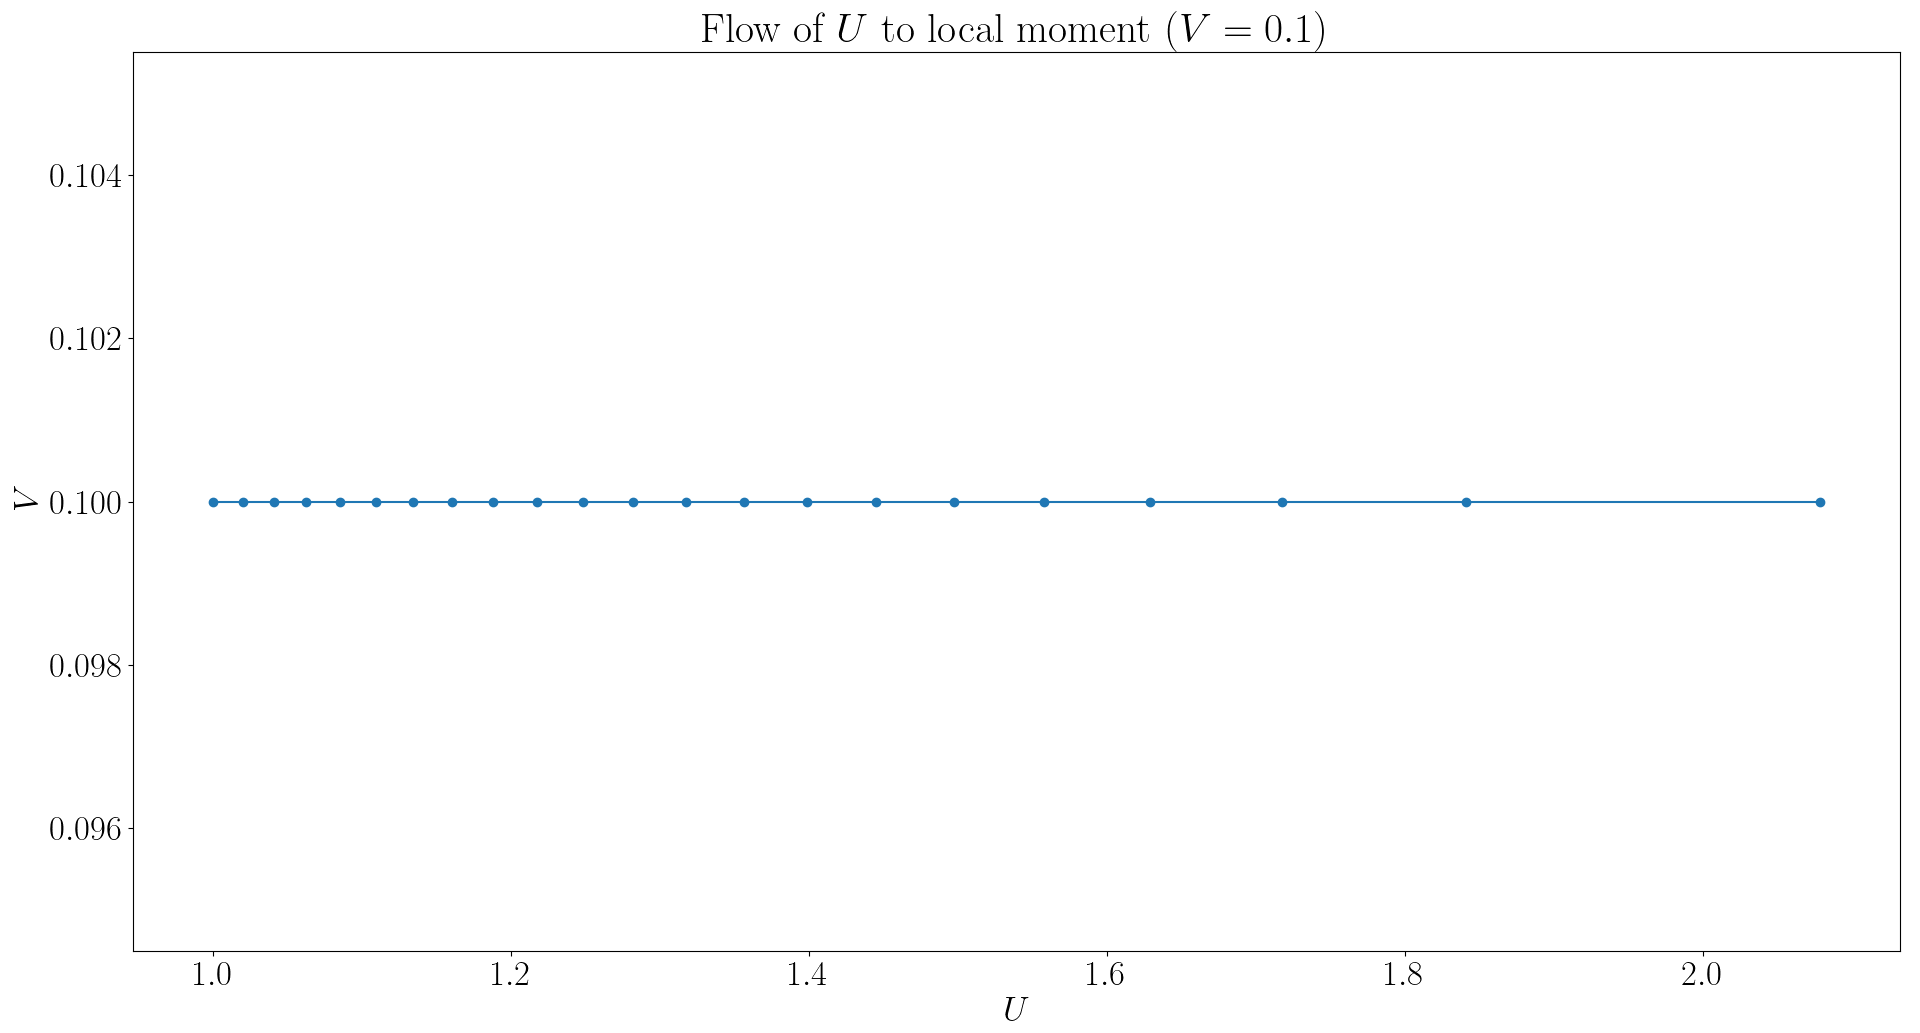
\includegraphics[scale=0.2]{fo2lm.png}}
% \begin{tabular}{cl}  
% \begin{tabular}{l}
% 	\hspace*{-30pt}\parbox{0.33\linewidth}{
% 		\vspace*{-10pt}
% 	\begin{itemize}\uncover<2->{\item \textbf{No separatrix} for the flows to the local moment} 
% 		\vspace*{10pt}
% 		\uncover<3>{\item Local moment forms at \textbf{finite \(U\)}.}
% \end{itemize}
%     }
%          \end{tabular}
%            &  \uncover<3>{ \begin{tabular}{c}
% 			   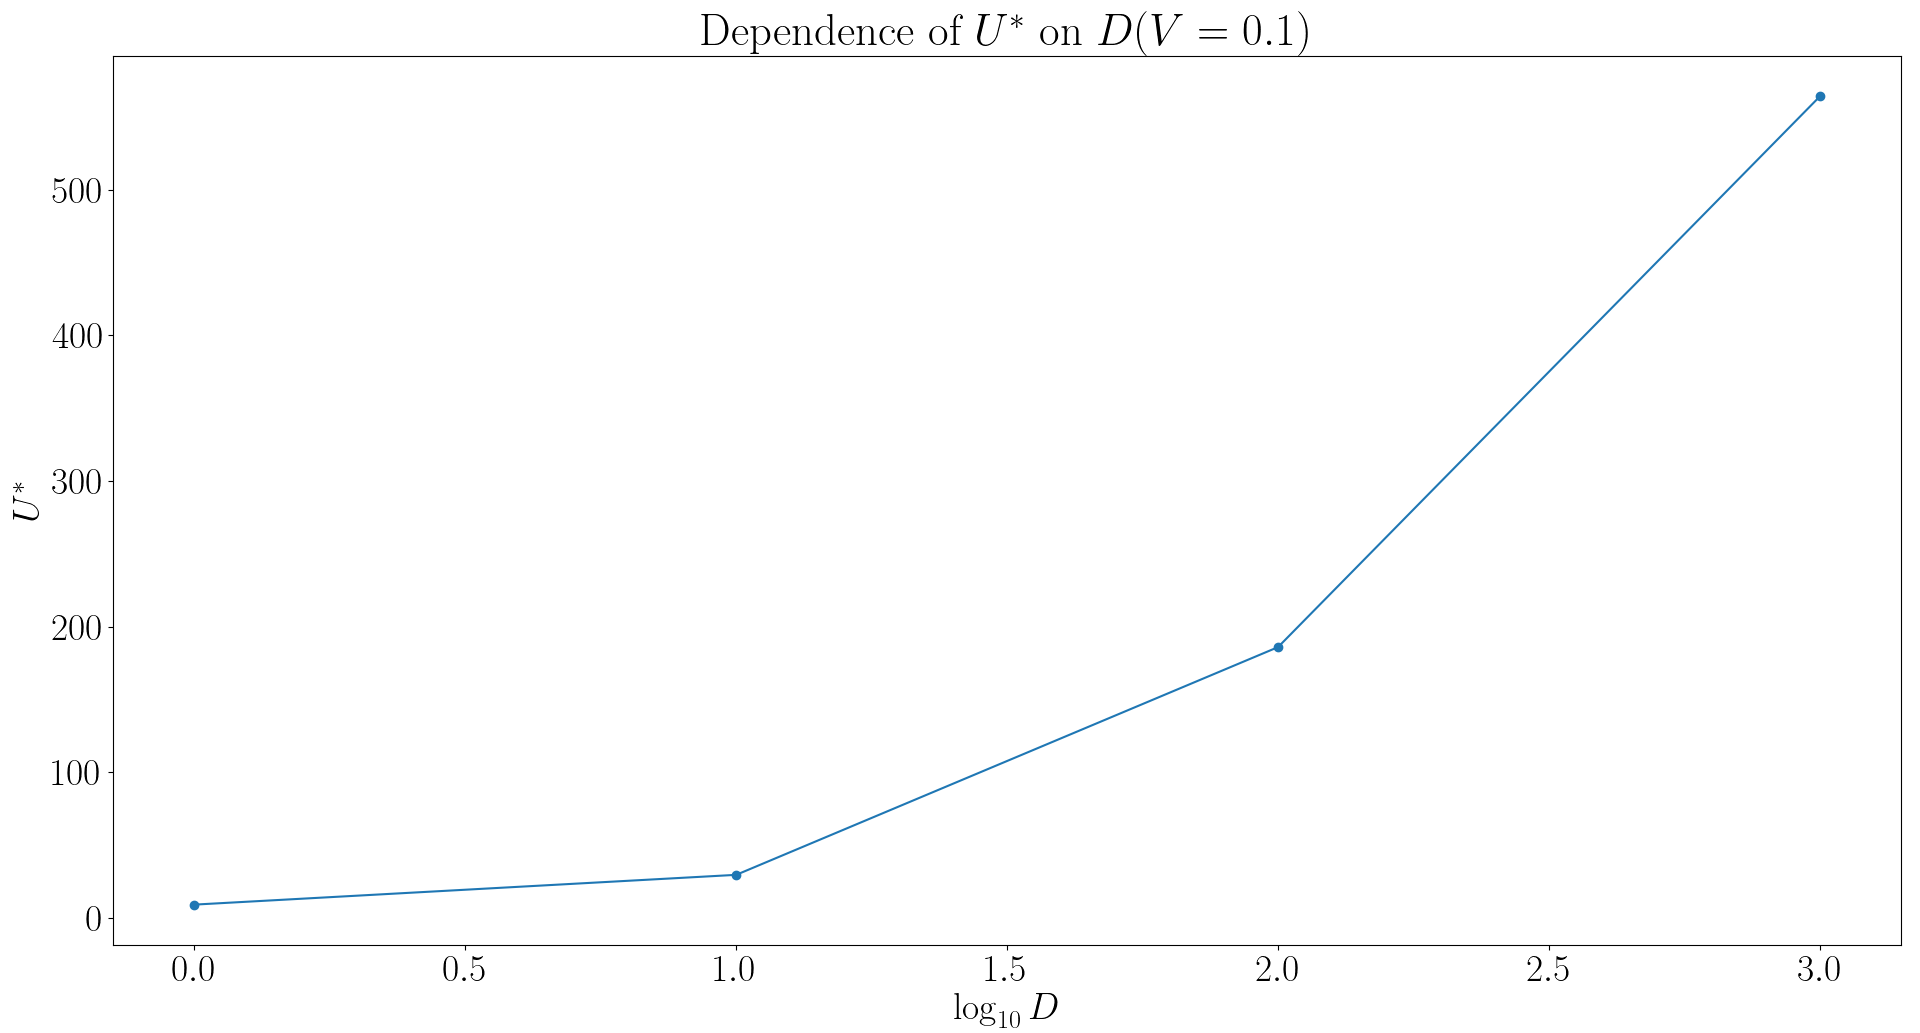
\includegraphics[scale=0.2]{UvsbareD.png}
% 	   \end{tabular}}\\
   
% \end{tabular}
% \end{frame}

% \begin{frame}[noframenumbering]{Results (\(\pmb{J>0}\))}
 
% \begin{tabular}{cl}  
% \begin{tabular}{l}
% \hspace*{-20pt}\parbox{0.5\linewidth}{
% \begin{itemize}
% \vspace*{-20pt}
% \item J now drives the flow towards strong-coupling fixed point.
% \vspace*{10pt}
% \item This is in contrast to the NRG flow diagram where \(\Delta \sim \frac{V^2}{U}\) was the driver of the flow.
% \end{itemize}
% }
% \end{tabular}
% & \begin{tabular}{c}
% \only<1>{    
% \centering 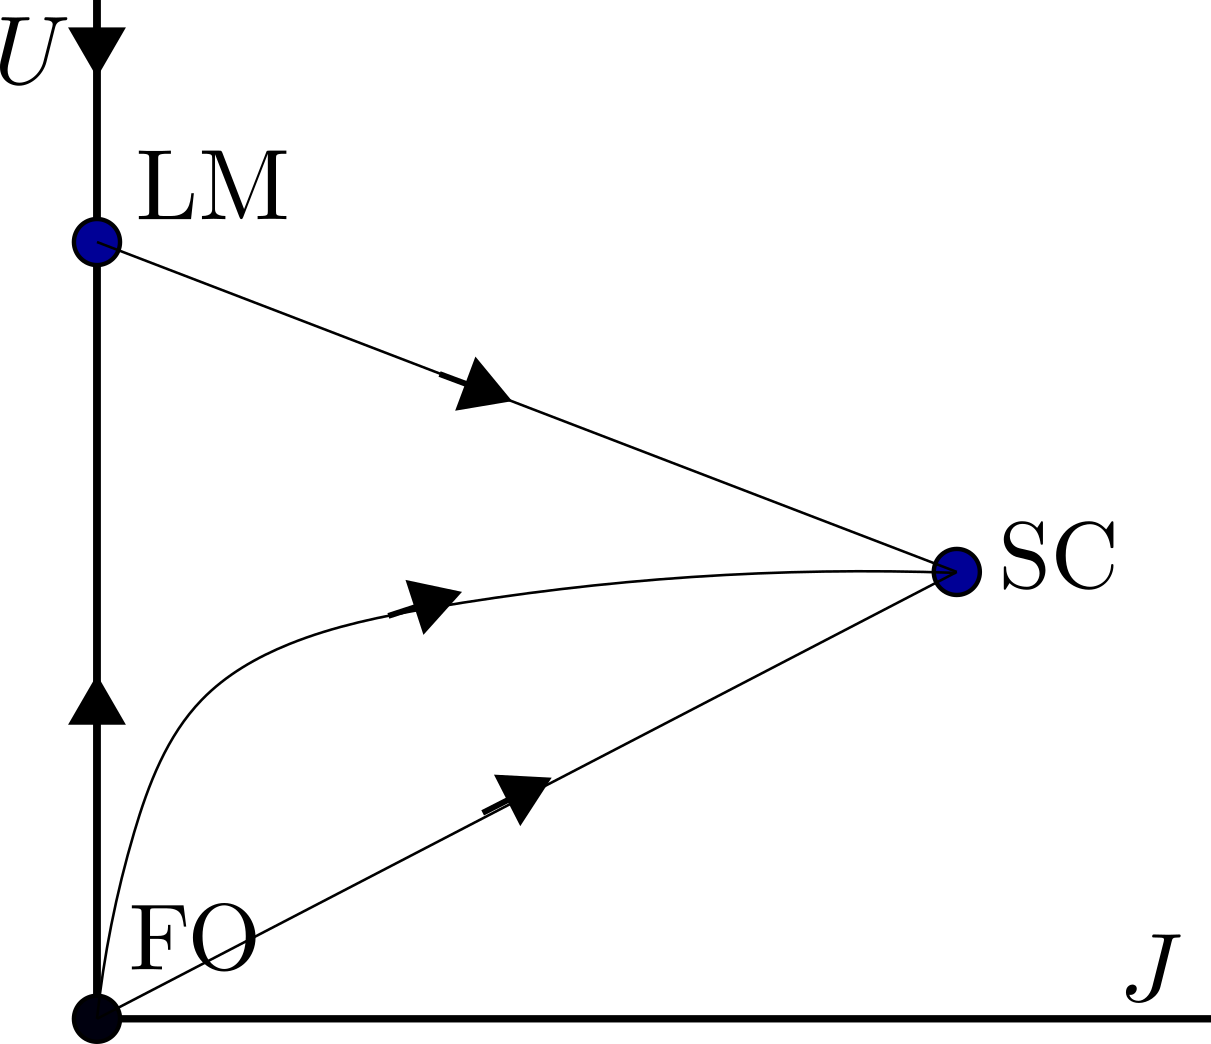
\includegraphics[scale=0.5]{schematic.png}
% }
% \only<2>{%
% 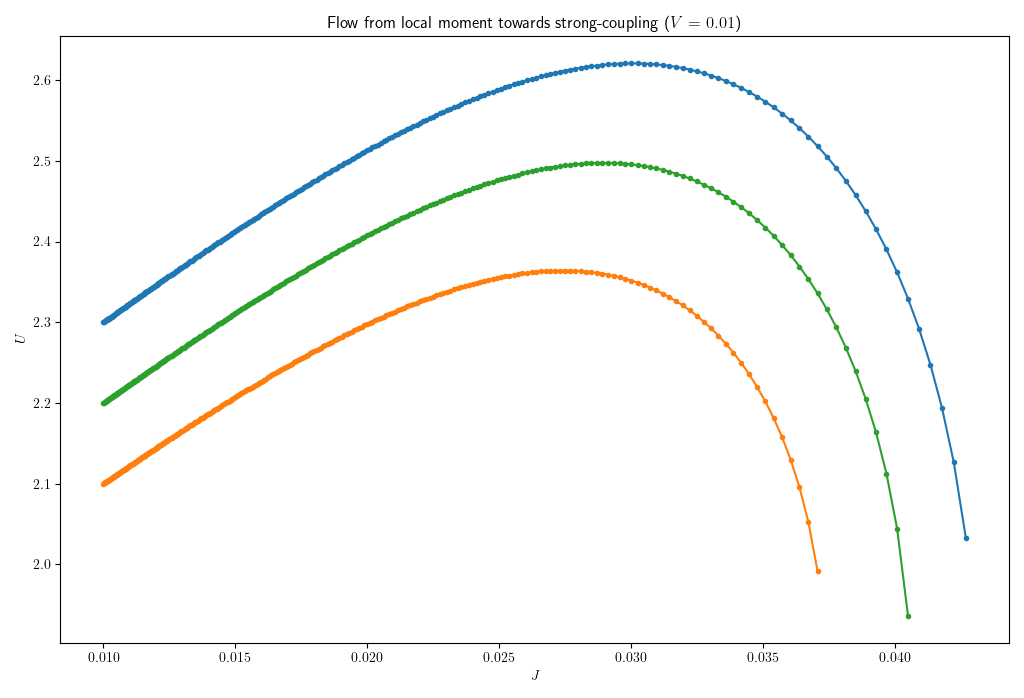
\includegraphics[width=0.35\textwidth]{lm2sc.png}\\
% \hspace*{5pt}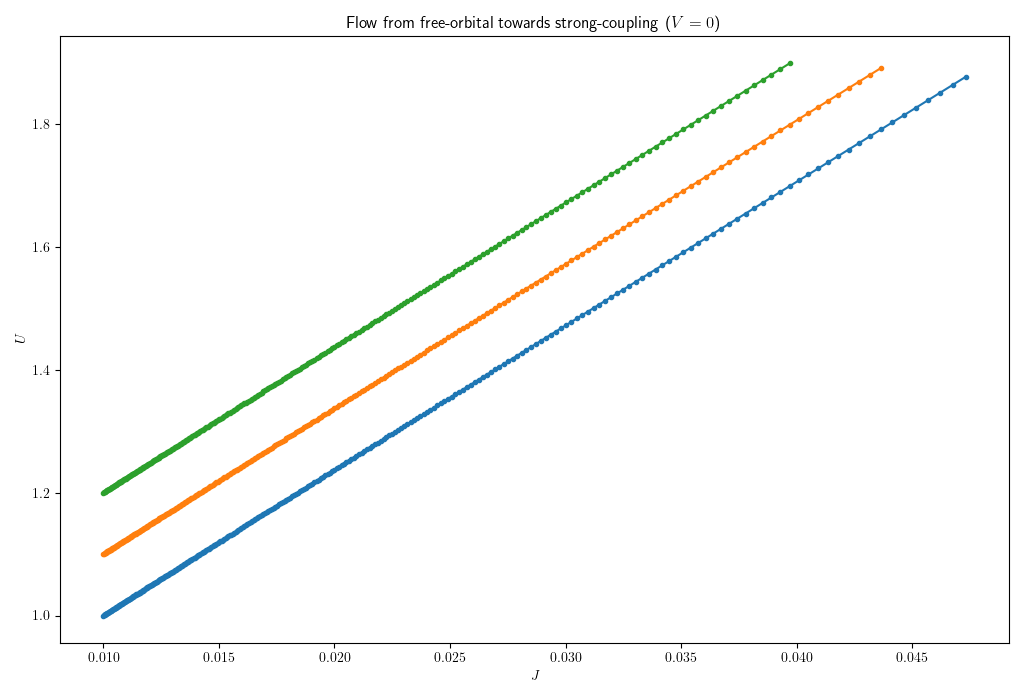
\includegraphics[width=0.35\textwidth]{fo2sc.png}
% }
% \end{tabular}
% \end{tabular}

\begin{frame}[noframenumbering]{Summary of Results}
	\vspace*{-5pt}
	\begin{figure}[htpb]
		\centering
		
\includegraphics[width=0.95\textwidth]{figures/summary.png}
	\end{figure}
\end{frame}

\begin{frame}[noframenumbering]{What's Next?}
\begin{itemize} 
\item Analytical expression for temperature-dependent Wilson ratio 
	\vspace{5pt}
\item Separating the contributions of various parts of the Kondo cloud to the spectral function
	\vspace{5pt}
\item Suggested by the generalized double-bracket form of URG, we can try to see if URG can be used as an optimizer.
	\vspace{5pt}
\item Since the zero-mode low-energy theory is an Anderson molecule (which can be exactly solved), it would be interesting to see if there is a transformation which converts the Anderson molecule to the Hubbard molecule.
	\vspace{5pt}
\item We can also check how using more feature-full baths (with non-trivial self-energy) can change the phase diagram.
	\vspace{5pt}
\item extensions to the Kondo and Anderson lattices, and hence to the problem of heavy Fermions
\end{itemize}
\end{frame}
\begin{frame}[noframenumbering]
	\LARGE \centering Thank You!
\end{frame}
\printbibliography
\end{document}
